\RequirePackage[l2tabu, orthodox]{nag}
\documentclass[10pt]{book}

% Language support
\usepackage[spanish, english]{babel}


% Thesis format
\usepackage[paperheight=24cm, paperwidth=17cm]{geometry}

% Graphics support
\usepackage{graphicx}
\graphicspath{{figures/}}

% Useful math features
\usepackage{amssymb}
\usepackage{amsmath}
\usepackage{bm}

% Alter geometry of the page headers:
\usepackage{fancyhdr} 

% Fancy tables
\usepackage{booktabs}

%Citations are numbered, sorted and consequtive lists compressed:
\usepackage[numbers, compress, sort]{natbib}

% Allow appendices in chapters:
\usepackage[toc]{appendix}

% Sans serif for section names:
\usepackage{sectsty}
\allsectionsfont{\sffamily}
\chapterfont{\LARGE \sffamily}

% Setting header height:
\headheight 14pt

% Setting text size:
\setlength{\textwidth}{12.3cm}
\setlength{\textheight}{18.5cm}

% Setting margins:
\setlength{\oddsidemargin}{-1in}
\setlength{\evensidemargin}{-1in}
\setlength{\topmargin}{-1in}
\addtolength{\oddsidemargin}{2.5cm}
\addtolength{\evensidemargin}{2.2cm}
\addtolength{\topmargin}{1.8cm}

% Parameters for fancy headers:
\pagestyle{fancyplain}
\renewcommand{\chaptermark}[1]{\markboth{\chaptername\ \thechapter.\ #1}{}}
\renewcommand{\sectionmark}[1]{\markright{\thesection\ #1}}
\lhead[\fancyplain{}{\thepage}]{\fancyplain{}{\rightmark}}
\rhead[\fancyplain{}{\leftmark}]{\fancyplain{}{\thepage}}
\cfoot{}

% Alter some LaTeX defaults for better treatment of figures.  Taken from
% http://mintaka.sdsu.edu/GF/bibliog/latex/floats.html
\renewcommand{\topfraction}{0.9}    % max fraction of floats at top
\renewcommand{\bottomfraction}{0.8} % max fraction of floats at bottom
\renewcommand{\textfraction}{0.1}   % allow minimal text w. figs

% Hyphenation:
\hyphenation{Ber-cea-nu Mar-chet-ti Ca-ru-sot-to}

% Abbreviations:
\newcommand*{\Lca}{\mathcal{L}}


\newcommand*{\la}{\langle}
\newcommand*{\ra}{\rangle}
\newcommand*{\abs}[1]{\vert #1 \vert}
\newcommand*{\bra}[1]{\langle #1 \vert}
\newcommand*{\ket}[1]{\vert #1 \rangle}
\newcommand*{\braket}[2]{\langle #1 \vert #2 \rangle}

%\newcommand*{\zb}{\bar{z}}
%\newcommand*{\e}{\epsilon}

\newcommand*{\rv}{\bm{r}}
\newcommand*{\kv}{\bm{k}}
\newcommand*{\kop}{\hat{\bm{k}}}


% \colvec{a}{b}
\newcommand*\colvec[2]{
  \begin{pmatrix}
    #1\\
    #2
  \end{pmatrix}
}

% \mat{a}{b}{c}{d}
\newcommand*{\mat}[4]{
  \begin{pmatrix}
    #1 & #2\\
    #3 & #4
  \end{pmatrix}
}

\newcommand*{\etal}{\emph{et al.}}

\DeclareMathOperator{\real}{Re}
\DeclareMathOperator{\imag}{Im}

%Landau chapter stuff
\DeclareMathOperator{\re}{Re}
\DeclareMathOperator{\im}{Im}
\DeclareMathOperator{\Tr}{Tr}
\DeclareMathOperator{\de}{d\!}
\DeclareMathOperator{\diag}{diag}
\DeclareMathOperator{\Res}{Res}
\DeclareMathOperator{\sgn}{sgn}
\DeclareMathOperator{\Det}{Det}
\DeclareMathOperator{\rank}{rank}

\newcommand{\vt}[1]{\mathbf{#1}}
%%%%

\DeclareMathOperator{\Ry}{\mathcal{R}y}

\newcommand{\noo}[1]{: \negthinspace {#1} \negthinspace :}

%OPO chapter stuff
\DeclareMathOperator{\tr}{tr}
\DeclareMathOperator*{\Simiq}{\simeq}
\DeclareMathOperator*{\To}{\to}

\newcommand{\vect}[1]{{\mathbf #1}}
\newcommand{\vectgr}[1]{{\boldsymbol#1}}    %Greek letter in bold
\newcommand{\Frac}[2]{\displaystyle\frac{#1}{#2}}
\newcommand{\MF}{\text{MF}}
%%%%%%%%%%

\begin{document}
\frontmatter

\thispagestyle{empty}

\begin{center}
{\Huge  Scattering and topological properties of \\ driven-dissipative quantum fluids\\}
\vspace{5.4cm}
{\large{TESIS DOCTORAL}}\\
\vspace{2.6cm}
{ \textsc{memoria presentada para optar al grado de \\ Doctor en Ciencias F\'{i}sicas\\
Universidad Aut\'{o}noma de Madrid\\
Departamento de F\'{i}sica Te\'{o}rica de la Materia Condensada\\
Programa de Doctorado\\
F\'{i}sica de la Materia Condensada y Nanotecnolog\'{i}a\\
day-of-week day month year\\ %TODO: update when defense date is known
$\,$\\$\,$\\por\\$\,$\\$\,$\\}
{\LARGE{Andrei Ciprian Berceanu}}\\$\,$ \\\textsc{nacido en Bucarest, Ruman\'{i}a en 1983}}
\end{center}
\newpage

\thispagestyle{empty}
\noindent {\large\bfseries Comisi\'{o}n:}\\[2ex]
  \parbox[t]{2.8cm}{Director:\\
                  Tribunal:
}~\parbox[t]{9cm}{Prof.\ dr.\ F.\ M.\ Marchetti (UAM) \\
Prof.\ dr.\ C.\ Tejedor (UAM) \\
Prof.\ dr.\ L.\ Vi\~{n}a (UAM) \\
Dr.\ A.\ Amo (CNRS, France) \\
Dr.\ J.\ J.\ Garc\'{\i}a-Ripoll (CSIC) \\
Dr.\ T.\ Ozawa (Universit\`{a} di Trento, Italy)
}

% TODO: check members of the committee

\vfill


\noindent
\begin{otherlanguage}{spanish}
El autor agradece el apoyo financiero de FP7 ITN ``Clermont4'' y
de la European Science Foundation (ESF) a trav\'{e}s de POLATOM Grant 4914.
\end{otherlanguage}
\vspace{\baselineskip}


\noindent
The author acknowledges financial support from FP7 ITN ``Clermont4'' and
from the European Science Foundation (ESF) through POLATOM Grant 4914.
\vspace{\baselineskip}


\begin{center}
\includegraphics[width=30mm]{uam_logo}  
\end{center}


\newpage

\thispagestyle{empty}

\phantom{text}

\vspace{2cm}

\begin{flushright}
  {\em Bunicilor mei.}
\end{flushright}

\newpage

\thispagestyle{empty}

%%% Local Variables:
%%% mode: latex
%%% TeX-master: "thesis_berceanu"
%%% End:



\tableofcontents
\mainmatter

\chapter{Introduction}

% TODO: insert chapter descriptions (see akhmerov)
% TODO: create abbreviations list
% GP: Gross-Pitaevskii
% TODO: mention \hbar = 1


\section{Preliminaries}
\label{sec:preliminary}

\subsection{Linear response theory}
\label{subsec:linear-response}

Let $\phi_0(\rv)$ be the steady state solution to the
GP equation in the time-independent trapping potential $U_0(\rv)$
%
\begin{equation}\label{eq:GP-atoms}
  H_{\text{GP}} \phi_0 = 0
\end{equation}
% 
with the GP Hamiltonian defined as\footnote{This section follows
  loosely the formalism presented in Ref.~\cite{9783540410478}.}
%
\begin{equation}\label{eq:GP-ham}
  H_{\text{GP}} \equiv -\frac{\nabla^2}{2m} + U_0 + gN_0\abs{\phi_0}^2 - \mu
\end{equation}
% 

This Hamiltonian describes a bosonic condensate of $N_0$ particles with
contact interactions quantified by $g$, and chemical potential $\mu$.

Now consider adding a small time-dependent perturbation on top of the
trap, giving $U(\rv,t)=U_0(\rv) + \delta U(\rv,t)$. We are interested
in the response of the condensate to this perturbation.  For weak
perturbations, we can perform a linearization of the GP equation
Eq.~\eqref{eq:GP-atoms} around the stationary solution $\phi_0$. This
approach is known in the literature as the ``linear response''
formalism.

The condensate wavefunction $\phi(\rv,t)$ evolves according to
%
\begin{equation}\label{eq:GP-atoms-evolution}
  i\partial_t \phi = \left[-\frac{\nabla^2}{2m} + U + gN_0 \abs{\phi}^2 - \mu\right] \phi
\end{equation}
% 
We assume a small deviation of the wavefunction from its initial
steady state
%
\begin{equation}\label{eq:ansatz-atoms}
  \phi(\rv,t) = \phi_0(\rv) + \delta\phi(\rv,t)
\end{equation}
% 
such that we can expand Eq.~\eqref{eq:GP-atoms-evolution} and keep only linear terms in $\delta\phi$ and $\delta U$. We get
%
\begin{equation}\label{eq:GP-atoms-lin}
  i\partial_t\delta\phi =  \left[-\frac{\nabla^2}{2m} + U_0-\mu\right]
  \delta\phi + 2 g N_0 \phi_0^{\star}\phi_0\delta\phi + gN_0\phi_0^2\delta\phi^{\star}
  +\delta U\phi_0
\end{equation}
% 
Note that Eq.~\eqref{eq:GP-atoms-lin} is not strictly linear due to
the coupling of $\delta\phi$ to $\delta\phi^{\star}$. To restore
linearity, we consider the functions $\delta\phi$ and
$\delta\phi^{\star}$ as being independent and write the linear system
%
\begin{equation}\label{eq:GP-atoms-system}
  i \partial_t \colvec{\delta\phi(\rv,t)}{\delta\phi^{\star}(\rv,t)}
  = \Lca_{GP} \colvec{\delta\phi(\rv,t)}{\delta\phi^{\star}(\rv,t)}
  + \colvec{S(\rv,t)}{-S^{\star}(\rv,t)}
\end{equation}
% 
where we have introduced the linear operator
%
\begin{equation}\label{eq:LGP}
  \Lca_{\text{GP}} = \mat{H_{\text{GP}}+gN_0\abs{\phi_0}^2}{g N_0 \phi_0^2}{-g N_0 \phi_0^{\star 2}}{-\left[H_{\text{GP}}+gN_0\abs{\phi_0}^2\right]^{\star}}
\end{equation}
% 
and the source term $S(\rv,t)=\delta U(\rv,t)\phi_0(\rv)$.  Note that
$\Lca_{\text{GP}}$ is not a Hermitian operator! The presence of the minus
sign in the second line is due to the fact that the particles obey
Bose statistics, as this is not present in the BCS theory.

The standard method of determining the time evolution of $\delta\phi$
is to expand it in the basis formed by the eigenvectors of
$\Lca_{\text{GP}}$.

There is a subtlety involved here, however, as in the general case
$\Lca_{\text{GP}}$ is not diagonalizable. It usually has too few
eigenvectors to span the whole functional space\footnote{We are
  referring to the $L^2 \times L^2$ space, with $L^2$ being the space
  of square-integrable complex functions.}.

The solution to this problem, detailed in Ref.~\cite{Castin_1998},
is to work in the subspace orthogonal to $\ket{\phi_0}$. It can be
shown that the component of the solution along $\ket{\phi_0}$ only
results in a change of phase of the total condensate wavefunction. For
the problems of interest in the rest of this manuscript, however, the
dimension of the space parallel to $\ket{\phi_0}$ that we must project
out is of order 1.

We now consider the eigenvalue equation for the operator $\Lca_{\text{GP}}$
%
\begin{equation}\label{eq:L-eigen}
  \Lca_{\text{GP}} \ket{\psi_k^R} = \epsilon_k \ket{\psi_k^R}
\end{equation}
% 
with $\ket{\psi_k^R}$ being the right eigenvector and $\epsilon_k$ its
corresponding eigenvalue
%
\begin{equation}\label{eq:psi-R}
  \ket{\psi_k^R} = \colvec{\ket{u_k}}{\ket{v_k}}
\end{equation}
% 
Similarly, we also introduce the left eigenvector, obeying
$\Lca_{\text{GP}}^{\dagger} \ket{\psi_k^L} = \epsilon_k^{\star} \ket{\psi_k^L}$,
and the orthonormality condition
$\braket{\psi_k^L}{\psi_q^R} = \delta_{k,q}$. 

Notice that $\Lca_{\text{GP}}$ and $\Lca_{\text{GP}}^{\dagger}$ are
connected by the unitary transformation\footnote{Note that this holds
  as long as the Hamiltonian $H_{\text{GP}}$ only contains real
  terms.}
%
\begin{equation}\label{eq:symmetry-1}
  \eta \Lca_{\text{GP}} \eta^{\dagger} = \Lca_{\text{GP}}^{\dagger}
\end{equation}
% 
where $\eta = \sigma_3 = \mat{1}{0}{0}{-1}$ is the third Pauli
matrix. We say that $\Lca_{\text{GP}}$ is $\eta$-Hermitian, meaning
that one can define a new scalar product
$\braket{\cdot}{\cdot}_{\eta} \equiv \braket{\cdot}{\eta \cdot}$ with a
different signature, such that
$\braket{\cdot}{\Lca_{\text{GP}} \cdot}_{\eta} =
\braket{\Lca_{\text{GP}} \cdot}{\cdot}_{\eta}$. The operator $\eta$ is
usually called the metric operator, and, not suprisingly in our case,
it is the same as the one of the scalar Klein-Gordon equation. A
pseudo-Hermitian operator usually also posesses antilinear symmetries,
and as we will see below this is also the case for
$\Lca_{\text{GP}}$. Interestingly, for operators with a real spectrum,
it can be shown that one can define another metric $\eta_+$, which
guarantees a positive-definite inner product, or, in other words,
$\braket{\psi}{\psi}_{\eta_+} > 0$ (provided $\psi \neq 0$ of
course). This can be used to formulate a probabilistic quantum theory
for the new wave-functions $\psi^R$ and $\psi^L$. For the general
theory and properties of pseudo-Hermitian operators, we point the
interested reader to Ref.~\cite{MOSTAFAZADEH_2010}.


Using Eq.~\eqref{eq:symmetry-1}, we get the general form of the left
eigen-vectors as
%
\begin{equation}\label{eq:psi-L}
  \bra{\psi_k^L} = {\cal N}_k \left( \bra{u_k},\, -\bra{v_k} \right)
\end{equation}
% 
with ${\cal N}_k$ a normalization factor.  We can chose
${\cal N}_k = \pm 1$ and group the eigenvalues of $\Lca_{\text{GP}}$
into 3 families, according to the quantity
%
\begin{equation}\label{eq:norms}
  n_k = \braket{u_k}{u_k} - \braket{v_k}{v_k}
\end{equation}
% 
We therefore have: the ``$+$'' family, corresponding to $n_k=+1$, the
``$-$'' family, such that $n_k=-1$ and the ``$0$'' family, with
$n_k=0$.

% In the absence of the added weak perturbation, the time evolution of
% mode $k$ is given by $\exp(-i\epsilon_k t)$, from which we get the
% dynamical stability condition $\imag{(\epsilon_k)} \leq 0$ for all
% $k$. Dynamical stability is important because it insures that small
% perturbations will not induce the condensate wavefunction to evolve
% far from its steady state value.

We are now ready to write the completeness relation
%
\begin{equation}\label{eq:completeness}
  \sum_k \ket{\psi_k^R} \bra{\psi_k^L} = \mathbb{I}
\end{equation}
% 
Using Eq.~\eqref{eq:completeness}, we can decompose any column vector
as\footnote{The modes in the ``$0$'' family do not appear in this
  expansion as their components live in the space orthogonal to the one
  of our solution.}
%
\begin{multline}\label{eq:decomposition}
  \colvec{\ket{l_1}}{\ket{l_2}} = \sum_{k \in ``+" \mbox{\scriptsize family}} \left[\braket{u_k}{l_1} - \braket{v_k}{l_2}\right]\colvec{\ket{u_k}}{\ket{v_k}}\\
  + \sum_{k \in ``-" \mbox{\scriptsize family}} \left[\braket{v_k}{l_2} - \braket{u_k}{l_1}\right]\colvec{\ket{u_k}}{\ket{v_k}}
\end{multline}
% 
There is now a further symmetry of $\Lca_{\text{GP}}$ that we can
exploit in our problem, a sort of time-reversal ``spin''-flip (or
particle-hole) symmetry, namely
%
\begin{equation}\label{eq:symmetry-2}
   \Theta \Lca_{\text{GP}} \Theta^{\dagger} = -\Lca_{\text{GP}}
\end{equation}
%
where $\Theta = \sigma_1 \cal{K}$, with $\sigma_1 = \mat{0}{1}{1}{0}$
the first Pauli matrix and $\cal{K}$ the complex conjugation
antilinear operator.

This results in a duality between the ``$+$'' family with eigenvectors
$(u_k, v_k)$ and energy $\epsilon_k$ and the ``$-$'' family with
eigenvectors $(v_{-k}^{\star}, u_{-k}^{\star})$ and energy
$-\epsilon_{-k}^{\star}$.

We can now finally project Eq.~\eqref{eq:GP-atoms-system} onto the
eigenvectors of $\Lca_{\text{GP}}$. Using the above-mentioned duality and
Eq.~\eqref{eq:decomposition}, we get
%
\begin{equation}\label{eq:phi-column-expansion}
  \colvec{\delta\phi(\rv,t)}{\delta\phi^{\star}(\rv,t)} = \sum_{k \in ``+" \mbox{\scriptsize family}}
  b_k(t) \colvec{u_k(\rv)}{v_k(\rv)}
  + b_{-k}^{\star}(t) \colvec{v_{-k}^{\star}(\rv)}{u_{-k}^{\star}(\rv)}
\end{equation}
% 
with the complex amplitudes $b_k$ satisfying 
%
\begin{equation}\label{eq:amplitudes-bk}
  i \frac{d}{dt}b_k(t) = \epsilon_k b_k(t) + s_k(t)
\end{equation}
% 
where we introduced
%
\begin{equation}\label{eq:amplitudes-sk}
  s_k(t) = \left( \bra{u_k} ,\, -\bra{v_k} \right) \colvec{\ket{S(t)}}{-\ket{S^{\star}(t)}}
\end{equation}
% 

\subsection{Cherenkov emission}
\label{subsec:cherenkov}

We now turn to applying the formalism developed in
Sec.~\ref{subsec:linear-response} to a concrete physical example,
inspired by Ref.~\cite{Carusotto_2006}. Consider a 2-dimensional
Bose-Einstein atomic condensate in a state with well-defined momentum,
described by the plane wave
$\psi_0 \exp \left( i \bm{k_0} \rv - \omega_0 t \right)$. Using our
previous notation, this corresponds to
%
\begin{equation}\label{eq:atom-initial}
  \phi_0(\rv) = \psi_0 \exp \left( i \bm{k_0} \rv \right)
\end{equation}
% 
and a chemical potential $\mu = \omega_0$. Since we have no trap,
$U_0(\rv)=0$, and Eq.~\eqref{eq:GP-atoms} reduces to
%
\begin{equation}\label{eq:atom-MF}
  \omega_0 - \left( \frac{k_0^2}{2m} + g \rho_0 \right) = 0
\end{equation}
% 
where we have introduced the condensate density
$\rho_0 \equiv N_0 \abs{\psi_0}^2$.  

We now intoduce a weak perturbation in the form of a localized defect
potential $\delta U(\rv, t) = V_d(\rv)$, which can represent for
instance a laser spot depleting a small area of the condensate.

Using Eq.~\eqref{eq:atom-MF}, the GP Hamiltonian becomes
$H_{\text{GP}} = -\frac{\nabla^2}{2m} - \frac{k_0^2}{2m}$ and the
source term
$S(\rv) = \psi_0 V_d(\rv) \exp \left( i \bm{k_0} \rv \right)$. We now
get the linear operator for our problem in the form
%
\begin{equation}\label{eq:ourL}
  \Lca = \mat{-\frac{\nabla^2}{2m} - \frac{k_0^2}{2m} + g\rho_0}{g N_0 \psi_0^2 \exp \left( 2 i \bm{k_0} \rv \right)}{- g N_0 \psi_0^{\star 2} \exp \left( - 2 i \bm{k_0} \rv \right)}{-\left[ -\frac{\nabla^2}{2m} - \frac{k_0^2}{2m} + g\rho_0 \right]}
\end{equation}
% 
Notice that, due to the presence of the off-diagonal exponential
terms, $\Lca$ does not commute with the momentum operator, which is
the generator of the spatial translation group. Luckily, however, we
can restore translational invariance by a simple unitary
transformation, as shown below.

First, a brief reminder of basic quantum mechanics. Using the standard
commutation relations, one can show that, for a constant wavevector
$\bm{k_0}$, the unitary operator\footnote{The hat symbol denotes
  operators in the relevant Hilbert space.}
%
\begin{equation}\label{eq:trans-oper}
  \hat{T}(\bm{k_0}) = \exp \left( -i \bm{k_0} \hat{\rv} \right)
\end{equation}
% 
performs a translation in momentum space,
$\hat{T}(\bm{k_0}) \ket{\bm{k}} = \ket{\bm{k} - \bm{k_0}}$, with the
ket $\ket{\bm{k}}$ representing a single particle state with
wavevector $\bm{k}$ such that
$\hat{\bm{k}} \ket{\bm{k}} = \bm{k} \ket{\bm{k}}$. Using the
definitions above, one can easily obtain the commutator
%
\begin{equation}\label{eq:trans-commutator}
  \left[ \hat{\bm{k}},\, \hat{T}(\bm{k_0}) \right] = -\bm{k_0}\hat{T}(\bm{k_0}) 
\end{equation}
% 
This allows us to rewrite the following expressions
\begin{align}\label{eq:products}
  \begin{split}
    \hat{T}^{\dagger}(\bm{k_0})\hat{\bm{k}}\hat{T}(\bm{k_0})& = \hat{\bm{k}} - \bm{k_0}\hat{\mathbb{I}}\\
    \hat{T}(\bm{k_0})\hat{\bm{k}}\hat{T}^{\dagger}(\bm{k_0})& = \hat{\bm{k}} + \bm{k_0}\hat{\mathbb{I}}  
  \end{split}
\end{align}

We now recognize the two exponentials in Eq.~\eqref{eq:ourL} as being
the real-space representation of $\hat{T}^2(\bm{k_0})$ and its
hermitian conjugate. This motivates us to define the following unitary
operator
%
\begin{equation}\label{eq:ucal}
  \hat{{\cal T}}(\bm{k_0}) = \mat{\hat{T}(\bm{k_0})}{0}{0}{\hat{T}^{\dagger}(\bm{k_0})}
\end{equation}
% 
such that a unitary transformation of our operator $\Lca$ now restores translational
symmetry. Indeed, one can see that
%
\begin{equation}\label{eq:translated-L}
  \hat{{\cal T}} \hat{\Lca} \hat{{\cal T}}^{\dagger} = \mat{\frac{\left(\kop + \bm{k_0}\right)^2}{2m} - \frac{k_0^2}{2m} + g\rho_0}{g N_0 \psi_0^2}{- g N_0 \psi_0^{\star 2}}{-\left[\frac{\left(\kop - \bm{k_0}\right)^2}{2m} - \frac{k_0^2}{2m} + g\rho_0 \right]}
\end{equation}
% 
where we have make use of Eqs.~\eqref{eq:products} and we have written
$\hat{\Lca}$ in a base-independent representation.  In the subspace of
momentum eigenstates $\ket{\kv}$, we can write the (right-)eigenvalue
equation corresponding to Eq.~\eqref{eq:translated-L} as
%
\begin{equation}\label{eq:right-eigen}
  \Lca_{\text{GP}} [k] \colvec{U_\sigma(k)}{V_\sigma(k)} = \epsilon_\sigma(k) \colvec{U_\sigma(k)}{V_\sigma(k)}
\end{equation}
% 
where we have recovered the matrix representation of
Eq.~\eqref{eq:LGP}, and introduced the notation
$\omega_\sigma(\kv) = \bm{v}_0 \kv + \epsilon_\sigma(k)$. Here
$\sigma = \pm$ labels the 2 different eigenmodes and we defined
$\bm{v}_0 \equiv \frac{\kv_0}{m}$ as the speed of the condensate.

Notice that the $k=0$ mode has only one eigenvector. However, one can
safely exclude it as this mode does not imply energy or momentum
transport. Excluding the $k = 0$ point, one can then solve
Eq.~\eqref{eq:right-eigen} and obtain the celebrated Bogoliubov
excitation spectrum
%
\begin{equation}\label{eq:bogoliubov}
  \epsilon_\sigma(k) = \sigma \left[\frac{k^2}{2m}\left(\frac{k^2}{2m} + 2 g \rho_0 \right) \right]^{\frac{1}{2}}
\end{equation}
% 
with $\sigma = \pm$. Notice that the complex amplitudes $U_\sigma(k)$,
$V_\sigma(k)$ only depend on the absolute value of $\kv$, while the
(real) spectrum of Eq.~\eqref{eq:translated-L}, $\omega_\sigma(\kv)$
is the Bogoliubov spectrum with an additional Galilean boost
$\bm{v}_0 \kv$.

As can be seen from Eq.~\eqref{eq:symmetry-2}, the 2 eigen-families
$\sigma$ and $-\sigma$ are linked by a duality, stemming from the
$\cal{P} \cal{T}$ symmetry\footnote{This can be actually formally
  proven after defining the parity and time-reversal operators
  corresponding to our problem. For details, see
  Ref.~\cite{MOSTAFAZADEH_2010}.} of the Bogoliubov operator $\Lca$.
We therefore drop the subscript and make the convention that
$\left( U,\, V \right) \equiv \left( U_{+},\, V_{+}
\right)$. Furthermore, making use of Eq.~\eqref{eq:symmetry-1}, we can
act with $\sigma_3$ on the eigenstates of $\Lca_{\text{GP}}$ to obtain
the ones of $\Lca_{\text{GP}}^{\dagger}$. 

This finally leads us to a biorthonormal basis
$\left\{ \ket{\psi_\sigma^R(\kv)},\, \ket{\psi_\sigma^L(\kv)} \right\}$
with 4 basis vectors
%
\begin{equation}\label{eq:biorthobasis}
  \left\{ \colvec{U(k)}{V(k)}, \colvec{V^{\star}(k)}{U^{\star}(k)}, \colvec{U(k)}{-V(k)}, \colvec{-V^{\star}(k)}{U^{\star}(k)} \right\} \bigotimes \ket{\kv}
\end{equation}
% 
which fulfills the orthonormality condition
%
\begin{equation}\label{eq:binormality}
  \braket{\psi_{\sigma^{\prime}}^L(\kv^{\prime})}{\psi_\sigma^R(\kv)} = \delta_{\sigma,\sigma^{\prime}} \delta^2(\kv - \kv^{\prime})
\end{equation}
% 
provided of course that we normalize in such a way that
$\abs{U(k)}^2 - \abs{V(k)}^2 = 1$, and the completeness relation
%
\begin{equation}\label{eq:bicompleteness}
  \sum_{\sigma = \pm} \int d^2 \kv \; \ket{\psi_\sigma^R(\kv)}\bra{\psi_\sigma^L(\kv)} = 1
\end{equation}
% 
In this basis, the spectral decomposition of
Eq.~\eqref{eq:translated-L} is of the diagonal form
%
\begin{equation}\label{eq:bidecomposition}
  \hat{{\cal T}} \hat{\Lca} \hat{{\cal T}}^{\dagger} = \sum_{\sigma = \pm} \int d^2 \kv \; \omega_\sigma(\kv) \ket{\psi_\sigma^R(\kv)}\bra{\psi_\sigma^L(\kv)}
\end{equation}
% 
The concrete form of $\Lca_{\text{GP}}[k]$, coupled with the
normalization condition Eq.~\eqref{eq:norms}, determines the
eigenvectors of the ``+'' family up to a phase factor. Indeed, one can
choose $\abs{U(k)} \pm \abs{V(k)} = f(k)^{\pm\frac{1}{4}}$, with 
%
\begin{equation}\label{eq:norms}
  f(k) = \frac{\frac{k^2}{2m}}{\frac{k^2}{2m} + 2g\rho_0}
\end{equation}
% 
It is now a trivial matter to solve the linearized evolution equation
Eq.~\eqref{eq:GP-atoms-system} for our problem. In particular, for a
localized static defect potential $V_d(\rv) = g_V \delta^2(\rv)$,

\section{Microcavity exciton-polaritons}
\label{sec:polaritons}


Consider the following (simplified) physical system. We have a bunch
of photons confined within the metalic mirrors of an optical cavity
which also contains a 2D semiconductor quantum well (QW), as shown in
Fig.~\ref{fig:cavity-polaritons}. The photons continuously create
electron-hole pairs, which go by the name of excitons, within the
QW. The excitons in turn recombine, emiting photons, which every so
often escape through the imperfect cavity mirrors. If one uses a
continuous wave laser to replenish the lost photons, a steady state
can eventually be reached where the pumping balances the losses. The
system is however in a driven-dissipative state, out of thermal
equilibrium.

Exactly describing the system of electrons, holes and photons, taking
into account their Coulomb interaction and the disorder created by
defects inside the QW, as well as imperfections in the mirrors would
not allow for much physical insight into this problem. We therefore
use a series of approximations in order to construct an effective
Hamiltonian description of the system.
%
\begin{figure}[tb]\centering
  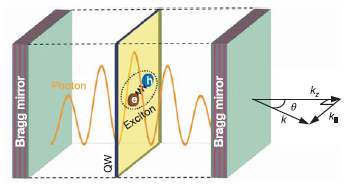
\includegraphics[width=.8\linewidth]{cavity}
  \caption{
    % 
    Pictorial representation of microcavity polaritons, as electron-hole pairs (excitons) inside a semiconductor quantum well, 
coupled with the photons trapped by the dielectric Bragg mirrors of the cavity. To excite the polariton mode with wave-vector $\kv$, a beam with incidence angle $\theta$ has to hit the microcavity, such that $k c = \omega \sin\theta$, with $\omega$ being the beam frequency.
From Ref.~\cite{Kasprzak_2006}.
    % 
}\label{fig:cavity-polaritons}
\end{figure}
% 
We start by writing down the kinetic energy of the photons
%
\begin{equation}\label{eq:cavity-energy}
  H_{C} = \sum_{\kv} E_C(k) a_{\kv}^{\dagger} a_{\kv}
\end{equation}
% 
where we've made use of the translational symmetry of the problem in
the $(x,y)$ plane and labeled the bosonic creation (annihilation)
operators $a_{\kv}^{\dagger}$ ($a_{\kv}$) by the in-plane momentum
$\kv$. The confinement along the $z$ direction leads to quantization
of the photon momentum $k_z = \frac{2 \pi N}{l_z}$, with
$N = 1,2,\dots$ indexing the longitudinal modes ($N=5$ in
Fig.~\ref{fig:cavity-polaritons}) and $l_z$ being the cavity width,
i.e. the distance between the mirrors. The cavity photon dispersion
for each of these modes is therefore $E_C(k) = v \sqrt{k^2 + k_z^2}$,
with $v$ the speed of light in the semiconductor. Expanding the square
root for $k \ll k_z$, one has
$E_C(k) \approx E_C(0) + \frac{k^2}{2m_{C}}$. We see that
cavity photons, as opposed to free-space photons, have a quadratic
dispersion with an effective mass
$m_{C} = \frac{E_C(0)}{v^2}$. For typical cavities used in
experiments, $m_{C}$ is of the order of $10^{-5}$ (free)
electron masses $m_e^0$.

We now turn our attention to the semiconductor QW. For simplicity,
consider a spin-polarized direct bandgap semiconductor such as GaAs,
so that we can neglect additional spin degrees of freedom. We further
assume that the dispersions of single particle states in the
conduction and valence bands have the quadratic form
$\varepsilon^c_{k} = \varepsilon_g/2 + k^2/(2m_e)$ and
$\varepsilon^v_{k} = - \varepsilon_g/2 - k^2/(2m_h)$, with
$\varepsilon_g$ the semiconductor bandgap and $m_e$ and $m_h$ the
effective masses for electrons and (heavy) holes. Excitons have a
typical extension $\lambda_X = \frac{\epsilon}{2\mu e^2}$ called the
(2D) exciton Bohr radius, with $\epsilon$ the static dielectric
constant, $e$ the electron charge and $\mu^{-1} = m_e^{-1} + m_h^{-1}$
their reduced mass. Their binding energy is called the exciton
Rydberg, defined as $\Ry_X = \frac{e^2}{\epsilon \lambda_X}$.

Defining $c_{\kv}^{\dagger}$ and $v_{\kv}$ as the operators creating
an electron in the empty conduction band, respectively a hole in the
filled valence band, we can write the electronic hamiltonian as
%
\begin{equation}\label{eq:coulomb-hamiltonian}
  H_{\text{el}} = \sum_{\kv} \left( \varepsilon^c_k c_{\kv}^{\dagger} c_{\kv} + \varepsilon^v_k v_{\kv}^{\dagger} v_{\kv} \right) + \frac{1}{2}\sum_{\bm{q}} V_q \left( \rho^e_{\bm{q}} \rho^e_{-\bm{q}} + \rho^h_{\bm{q}} \rho^h_{-\bm{q}} -2 \rho^e_{\bm{q}} \rho^h_{-\bm{q}}\right)
\end{equation}
% 
Here we have introduced the electron and hole densities,
$\rho^e_{\bm{q}} = \sum_{\kv} c_{\kv + \bm{q}}^{\dagger} c_{\kv}$ and
$\rho^h_{\bm{q}} = \sum_{\kv} v_{\kv} v_{\kv + \bm{q}}^{\dagger}$. The
matrix element of the Coulomb potential
$V_q = \frac{e^2}{2 \epsilon A q}$ depends on cavity quantization area
$A$, but this dependence drops out when passing from discrete sums
over states to intragrals over $\kv$.

Finally, the last ingredient of our microscopic description concerns
the interaction between electrons and photons. Making use of the
dipole and rotating wave approximations, we have
%
\begin{equation}\label{eq:dipolar-inter}
  H_{\text{dipole}} = \sum_{\kv, \bm{q}} G(q) \left( a_{\bm{q}}^{\dagger} v_{\kv + \bm{q}}^{\dagger} c_{\kv} + \text{H.c.}\right)
\end{equation}
% 
with the strength
$G(q) = e \mu_{\text{cv}}\sqrt{\frac{E_C(q)}{2\epsilon A l_z}}$
written in the dipole gauge, where $\mu_{\text{cv}}$ is the inter-band
dipole matrix element.

We are interested in an approximate description of the problem where
we can consider the excitons as fundamental quasiparticle excitations
from the ground state of the semiconductor and treat the Coulomb term
in Eq.~\eqref{eq:coulomb-hamiltonian} as an effective exciton-exciton
interaction. We then couple the resulting excitons to light, and
obtain the so-called \textbf{weakly interacting boson model} for
polaritons. The name stems from the fact that, at moderate
electron-hole densities, one can assume excitons to behave esentially
as bosons, and describe them using the Bose creation and annihilation
operators $b_{\kv}^{\dagger}$ and $b_{\kv}$. Therefore, making an Usui
transformation and truncating the interaction terms at fourth order
results in the following three-part effective Hamiltonian
%
\begin{equation}\label{eq:total-ham}
  H_{\text{eff}} = H_0  + H_{\text{XX}} + H_{XC}^{\text{sat}}
\end{equation}
% 
where we have defined
\begin{align}
  H_0 & =\sum_{\kv}\left(a_{\kv}^{\dagger},\, b_{\kv}^{\dagger}\right)\mat{E_C(k)}{\Omega_R}{\Omega_R}{E_X(k)}\colvec{a_{\kv}}{b_{\kv}}\label{eq:polariton-ham}\\
  H_{\text{XX}} & =\frac{1}{2}\sum_{\kv,\kv^{\prime},\bm{q}}U_{\kv - \kv^{\prime},\bm{q}}b_{\kv + \bm{q}}^{\dagger}b_{\kv^{\prime} - \bm{q}}^{\dagger}b_{\kv^{\prime}}b_{\kv}\label{eq:interaction-ham}\\
  H_{XC}^{\text{sat}} & =-\frac{\Omega_R}{\rho_{\text{sat}}A}\sum_{\kv,\kv^{\prime},\bm{q}}\left(b_{\kv^{\prime}-\bm{q}}^{\dagger}b_{\kv + \bm{q}}^{\dagger}b_{\kv}a_{\kv^{\prime}} + \text{H.c.}\right)\label{eq:saturation-ham}
\end{align}
$H_0$ contains the kinetic energy of the excitons and cavity photons,
as well as their harmonic coupling, ie. the conversion of an exciton
to a cavity photon at the Rabi frequency $\Omega_R$, which depends on
the overlap between the wavefunctions of the exciton and photon and
$\mu_{\text{cv}}$. Eq.~\eqref{eq:polariton-ham} can be diagonalized by
means of a unitary transformation of the form
%
\begin{equation}\label{eq:hopfield-trans}
  \colvec{p_{\kv}}{u_{\kv}} = \mat{X_k}{C_k}{-C_k}{X_k} \colvec{b_{\kv}}{a_{\kv}}
\end{equation}
% 
The normal modes of $H_0$ are called \textbf{upper and lower polaritons} and
correspond to the Bose operators $u_{\kv}$ and $p_{\kv}$, with
eigen-energies
%
\begin{figure}[tb]\centering
  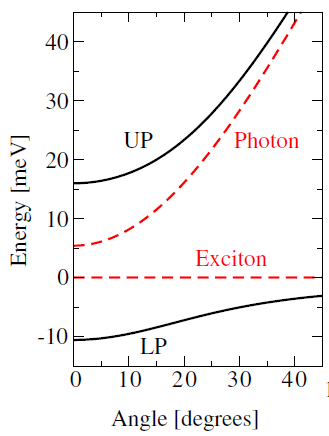
\includegraphics[width=.5\linewidth]{polariton_dispersion}
  \caption{
    % 
    Dispersion relation for the two polaritonic branches (UP, LP) as a function of emission angle $\theta$ of photons outside the cavity. This angle is connected to the momentum $k$ of polaritons inside the cavity by the relation $ck = E_{\text{LP}}(k) \sin \theta$. The exciton and cavity photon dispersions are depicted with dashed (red) lines. Notice the very sharp dispersion of the polaritons compared to excitons, due to the light mass of their photonic component.
From Ref.~\cite{Keeling_2007}.
    % 
}\label{fig:polariton-dispersion}
\end{figure}
% 
\begin{equation}\label{eq:polariton-dispersion}
  E_{\text{UP,LP}}(k) = \frac{1}{2}\left(E_C(k) + E_X(k)\right) \pm \frac{1}{2}\left[\left(E_C(k) - E_X(k)\right)^2 + 4 \Omega_R^2\right]^{1/2}
\end{equation}
% 
whereas the Hopfield coefficients appearing in Eq.~\eqref{eq:hopfield-trans} are
\begin{align}
  X_k & =\left[1 + \left(\frac{\Omega_R}{E_{\text{LP}}(k) - E_C(k)}\right)^2\right]^{-1/2}\label{eq:hopfield-X}\\
  C_k & =-\left[1 + \left(\frac{E_{\text{LP}}(k) - E_C(k)}{\Omega_R}\right)^2\right]^{-1/2}
\end{align}
The two branches of the polaritonic dispersion relation are shown in
Fig.~\ref{fig:polariton-dispersion}, together with the dispersions of
the cavity photons and excitons.

Note that the 1s-exciton energy can be approximated as
$E_X(k) = E_X(0) + \frac{k^2}{2M}$, with the exciton mass
$M = m_e + m_h$ of the order of the electron mass and
$E_X(0) = \varepsilon_g - \Ry_X$. Since, as we have already noted, $M$
is several orders of magnitude larger than the cavity photon mass
$m_{C}$, one can in practice neglect the momentum dependence
of the excitonic dispersion and consider it to be flat. Furthermore,
we can agree to measure energies starting from $E_X(0)$ and denote the
detuning between exciton and photon bands as
$\delta \equiv E_C(0) - E_X(0)$. For zero detuning ($\delta = 0$), the
splitting between the two polariton branches is $2\Omega_R$. In order
to tune $\delta$ in experiments, one tipically builds the cavity
mirrors with a wedge.

Also note that the spectrum in Fig.~\ref{fig:polariton-dispersion} is
represented as a function of the angle $\theta$ of emission of a
photon out of the cavity, as depicted in
Fig.~\ref{fig:cavity-polaritons}. Conservation of in-plane momentum
and photon frequency dictates that a laser beam coming in at an angle
$\theta$ and frequency $\omega$ resonantly excites a microcavity mode
with wave vector $k_{\parallel} = \frac{\omega}{c}\sin(\theta)$.

$H_{\text{XX}}$ quantifies the effective repulsive exciton-exciton
interaction, with a momentum-dependent strength
$U_{\kv - \kv^{\prime},\bm{q}}$ that can be calculated from the
Coulomb exchange term in the Born approximation. A further
approximation, for wave vectors much smaller than $\lambda_X^{-1}$, is
to reduce $U_{\kv - \kv^{\prime},\bm{q}}$ to a contact potential
$g_X \equiv \frac{1}{2} U_{\bm{0},\bm{0}} =
\frac{6e^2\lambda_X}{2A\epsilon}$. As a result $g_X$ physically
represents the interaction between two excitons in the same
single-particle momentum eigenstate $\ket{\kv}$.

Finally, the last term of Eq.~\eqref{eq:total-ham},
$H_{\text{XC}}^{\text{sat}}$, can be interpreted as a saturation
effect due to the Pauli exclusion principle underlying the fermionic
character of the excitons. The exciton saturation density
$\rho_{\text{sat}} = \frac{7}{16\pi\lambda_X^2}$ for the problems we
will be treating in the remainder of this manuscript can be considered
large enough to justify neglecting this anharmonic contribution to the
total Hamiltonian.

It is noteworthy to remark that Hamiltonian Eq.~\eqref{eq:total-ham}
does not include any disorder. We have already mentioned that there
are two distinct disorder classes in this problem. One is the
excitonic disorder, acting on length scales of around 10 nm, which
tipically affects the exciton oscillator strengths, but not the
spatial polaritonic density. This type of disorder stems from
variations in the QW thickness as well as alloy imperfections and is
typically not strong enough to dissociate excitons. Neglecting
excitonic disorder also implies that each localized exciton state
couples to precisely one extended photon state. The resulting
polaritons are then nothing but the superposition of these excitonic
and photonic states.

Photonic disorder, on the other hand, acts on lengthscales
$\ell_{C} = (m_{C}\Omega_R)^{-1/2}$ on the order of microns (see
Tab.~\ref{tab:GaAs-params}) and therefore can disrupt the polariton
density profile. It is normally caused by imperfections in the cavity
mirrors, which can act as scattering centers for the polaritons, and
can be included in the Hamiltonian as an additional external
potential. We will see some eloquent examples of polariton scattering
in the following chapters. Typical decay rates for excitons
($\gamma_X$) and cavity photons ($\gamma_C$) in GaAs-based
microcavities are also shown in Tab.~\ref{tab:GaAs-params}.

Last but not least, one should mention the validity limitations of the
weakly interacting boson model for polaritons. Its derivation, by
means of the Usui transformation, implies an expansion of the original
fermionic operators from Eq.~\eqref{eq:coulomb-hamiltonian} in powers
of bosonic operators, having as small parameter the number of excitons
per Bohr radius $\lambda_X$. Truncating the series results in an upper
bound on the exciton density of the order of $1/\lambda_X^2$. At
higher densities, an electron-hole plasma-like state is formed, with a
a qualitatively different behaviour.  We see that this model is
particularly useful for the case when the dominant interaction is the
Coulomb repulsion between the excitons.

For temperatures smaller than the Rabi splitting between the two
polariton branches, we can neglect the upper polaritons and project
Eq.~\eqref{eq:total-ham} on the basis of lower-polariton states
only. Employing the approximations we just mentioned, we obtain the
lower-polariton Hamiltonian
%
\begin{equation}\label{eq:LP-ham}
  H_{\text{LP}} = \sum_{\kv} E_{\text{LP}}(k) p_{\kv}^{\dagger} p_{\kv} + \sum_{\kv,\kv^{\prime},\bm{q}} V^{\text{eff}}_{\kv,\kv^{\prime},\bm{q}}\, p^{\dagger}_{\kv + \bm{q}} p^{\dagger}_{\kv^{\prime} - \bm{q}} p_{\kv} p_{\kv^{\prime}}
\end{equation}
% 
where the strength of the repulsive interaction between lower
polaritons now depends on in-plane momentum through the Hopfield
coefficients\footnote{The interaction strength $g_X$ can usually be
  rescaled to 1 by a simple transformation.}
%
\begin{equation}\label{eq:g-eff}
  V^{\text{eff}}_{\kv,\kv^{\prime},\bm{q}} = g_X X_{\kv + \bm{q}}X_{\kv^{\prime}}X_{\kv^{\prime} - \bm{q}}X_{\kv}
\end{equation}
% 
Physically, the quantities $\abs{X_k}^2$ and $\abs{C_k}^2$ are the
excitionic and photonic fractions of the lower lower polariton
mode. Their momentum dependence is not very pronounced, as for
$\delta = 0$, $X_k$ is between $1/\sqrt{2}$ and $1$ and if we are also
at normal incidence, meaning $\kv = 0$, than the light and matter
content of lower polaritons are each equal to $1/2$.

Consider now the low-temperature case, where the polaritons form a
BEC-like condensate in the momentum eigenstate $\ket{\kv}$. In this
case, since we have the macroscopic ocupation of a single particle
state, we can follow the standard Bogoliubov prescription and treat
the operator $p_{\kv}$ as a classical wavefunction, which we will
denote by $\psi_{\kv}$. The time-evolution of this classical object is
a Gross-Pitaevksii-like equation obtained from Heisenberg's equation
of motion
$i \partial_t \psi_{\kv}(t) = \left[\psi_{\kv}(t),\, H_{\text{LP}}\right]$.
Since polariton condensates are intrinsically out-of-equilibrium
systems, one also had to add additional terms in order to describe
pumping and losses. We therefore get a driven-dissipative mean-field
equation, which in momentum space reads
%
\begin{multline}\label{eq:mom-GPE}
  i\partial_t\psi_{\kv} = \left[E_{\text{LP}}(k) - \frac{i}{2} \gamma_k\right]\psi_{\kv} + \sum_{\kv_1,\kv_2} g_{\kv,\kv_1,\kv_2} \psi^{\star}_{\kv_1 + \kv_2 - \kv} \psi_{\kv_2} \psi_{\kv_1}\\
  + C_k f_p \exp{\left(-i \omega_pt\right)} \delta_{\kv,\kv_{p}}
\end{multline}
% 

%%%%%%

To get a more quantitative idea of the physics involved, it is worth
describing realistic samples typically used in state-of-the-art
experiments. Instead of simple metallic mirrors, such microcavities
are usually bound by a series of up to around 20 distributed Bragg
reflectors (DBRs), which are alternating dielectric layers of
thickness $\lambda/4$ and different refractive indices, achieving a
total reflectivity of over $99.9$\%. Multiple CdTe or GaAs QWs of
approximately $8~$nm thickness are placed inside the cavity of length
$l_z = 2\lambda \sim 1~\mu$m, at the antinodes (maxima) of the
photonic field, in order to maximize the coupling between excitons and
photons. Typical values of the relevant parameters for GaAs-based
microcavities are shown in Tab.~\ref{tab:GaAs-params}. As a sidenote,
one can see that for these values, the ratio between saturation and
Coulomb interaction
$\frac{\Omega_R}{g_X \rho_{\text{sat}}} \simeq 0.1$, hereby justifying
our assumption that we can neglect the anharmonic Hamiltonian
Eq.~\eqref{eq:saturation-ham}.
%
\begin{table}
  \centering
  \begin{tabular}{@{}ll@{}} \toprule
    QW & Cavity \\ \midrule
    $\epsilon \simeq 13$ &  $E_C(0) \simeq E_X(0) \simeq 1.53$~eV\\
    $m_e = 0.063m^0_e$    &  $\delta \in [-10,10]$~meV\\
    $m_h = 0.3m^0_e$      &  $m_{C} = 2.3\times 10^{-5} m^0_e$ \\
    $\lambda_X \simeq 7$~nm   & $\ell_{C} = 0.868~\mu$m\\
    $\Ry_X \simeq 17$~meV &  $\Omega_R \simeq 2.2$~meV \\
    $\gamma_X \sim \mu$eV &  $\gamma_C = 0.1$~meV \\ 
    $g_X \simeq 5\times10^{-3}$~meV($\mu$m)$^2$ &  $A = 10^4~\mu$m$^2$\\
    $\rho_{\text{sat}} \simeq 2842~$($\mu$m)$^{-2}$ &  $l_z \sim 1~\mu$m\\ \bottomrule
  \end{tabular}
  \caption{Typical parameters of a microcavity containing GaAs QWs, from Ref.~\cite{9783642241857}. Left column shows values concerning the QW while the right one refers to the microcavity.}
  \label{tab:GaAs-params}
\end{table}
%


%TODO: explanation of terms
%TODO: add defect potential
%TODO: real space driven-dissipative GPE
%TODO: different types of pumping
%TODO: mean-field equations, U(1)
%TODO: OPO
%TODO: add references
%TODO: anticrossing mention in disp fig, strong coupling
%TODO: polaritons = photons dressed by matter
%TODO: directly excited by laser and detected via reflection/transmission 




%%% Local Variables:
%%% mode: latex
%%% TeX-master: "../thesis_berceanu"
%%% End:

%%%%%%%%%%%%%%%%%%%%%%%%%%%%%%%%%%%
% Key                | Occurences | 
%--------------------+------------| 
% Cancellieri_2010   |         10 | 
% Wouters_2010 (*)   |          5 | 
% Astrakharchik_2004 |          5 | 
% Ciuti_2005         |          5 | 
% Amo_2009 (*)       |          4 | 
%%%%%%%%%%%%%%%%%%%%%%%%%%%%%%%%%%%


\chapter{Drag in a resonantly pumped polariton fluid}
\label{cha:drag}

\section{Introduction}
\label{sec:intro}

Out of equilibrium quantum fluids such as polaritons in semiconductor
microcavities are being the subject of an intensive study. Microcavity
polaritons, the quasiparticles resulting from the strong coupling of
cavity photons and quantum well excitons, have the prerogative of
being easy to both manipulate, via an external laser, and detect, via
the light escaping from the cavity~\cite{9780199228942}. In
particular, resonant excitation allows the accurate tuning of the
fluid properties, such as its density and current. However, the
polariton lifetime being finite establishes the system as
intrinsically out of equilibrium: An external pump is needed to
continuously replenish the cavity of polaritons, that quickly, on a
scale of tens of picoseconds, escape.

Recently, the superfluid properties of a resonantly pumped polariton
quantum fluid in the pump-only configuration --- i.e., where no other
states aside the pump one are occupied by, for example, parametric
scattering --- have been actively investigated both experimentally and
theoretically~\cite{Carusotto_2004,Ciuti_2005,Amo_2009,Cancellieri_2010,Pigeon_2011,Amo_2011,Nardin_2011,Sanvitto_2011}. This
pumping scheme, differently from other cases, such as the resonant
optical parametric oscillator regime and the non-resonant pumping
scheme, creates a polariton fluid that, inside the pump spot, is not
characterised by a free phase. In contrast, the phase of the pump
state is locked to the one of the external pumping
laser. Nevertheless, it has been
predicted~\cite{Carusotto_2004,Ciuti_2005} and
observed~\cite{Amo_2009} that scattering can be suppressed below a
critical velocity, where the system displays superfluid behaviour,
similar to what has been predicted by the Landau criterion for
equilibrium superfluid condensates. Furthermore, a fixed phase clearly
prevents the formation of phase dislocations, such as vortices and
solitons. For this reason, it has been suggested~\cite{Pigeon_2011}
and experimentally realised~\cite{Amo_2011} that the defect can be
located just outside the pump spot, where the hydrodynamic nucleation
of vortices, vortex-antivortex pairs, arrays of vortices, and solitons
can be observed when the fluid collides with the extended
defect. Similarly, nucleation of vortices in the wake of the obstacle
has been observed in pulsed experiments
~\cite{Nardin_2011,Sanvitto_2011}.

In a conservative quantum liquid flowing past a small defect, the
Landau criterion for superfluidity links the onset of dissipation at a
critical fluid velocity with the shape of the fluid collective
excitation spectrum~\cite{9780198507192}. In particular, for weakly
interacting Bose gases, the dispersion of the low-energy excitation
modes being linear implies that the critical velocity for superflow
coincides with the speed of sound $c_s$. Clearly, this is strictly
correct only for vanishingly small
perturbations~\cite{Astrakharchik_2004}, while for a defect with finite
size and strength, the critical velocity can be smaller than
$c_s$~\cite{Onofrio_2000,Ianeselli_2006}.

However, even for perturbatively weak defects, in out-of-equilibrium
systems, where the spectrum of excitations is complex, the validity of
the Landau criterion has to be
questioned~\cite{Szyma_ska_2006,Wouters_2010,Cancellieri_2010}. In the
particular case of coherently driven polaritons in the pump-only
configuration, it has been predicted~\cite{Carusotto_2004,Ciuti_2005}, and
later observed~\cite{Amo_2009}, that scattering is suppressed at either
strong enough pump powers or small enough flow velocities. Yet, on 
closer scrutiny, it has been shown that, despite the apparent validity
of the Landau criterion, the system always experiences a residual drag
force even in the limit of asymptotically large
densities~\cite{Cancellieri_2010} or small velocities. This result has
been proven by numerically solving the Gross-Pitaevskii equation
describing the resonantly-driven polariton system in presence of a
non-perturbative extended defect. Here, the drag force exerted by the
defect on the fluid has been shown to display a smooth crossover from
the subsonic to the supersonic regime, similar to what it has been
found in the case of non-resonantly pumped
polaritons~\cite{Wouters_2010}. In this Chapter, we find an even richer
phenomenology for the dependence of the drag force on the fluid
velocity and two different kinds of crossovers from the sub- to the
supercritical regime. Furthermore, we show that the origin of the residual
drag force, which, in agreement with Ref.~\cite{Cancellieri_2010}, lies
in the polariton lifetime only, can be demonstrated even within a
linear response approximation.

More specifically, we apply the linear response theory
to analytically evaluate the drag force exerted by the coherently
driven polariton fluid in the pump-only configuration on a point-like
defect. To simplify the formalism, we restrict our analysis to the
case of resonant pumping close to the bottom of the lower polariton
dispersion, where the dispersion is quadratic. Here, the properties of
the collective excitation spectrum have been shown to be uniquely
determined by three parameters only~\cite{Ciuti_2005}: the fluid
velocity $v_p$, the interaction-renormalised pump detuning $\Delta_p$,
and the polariton lifetime $\kappa$. In particular, the sign of the
detuning $\Delta_p$ determines three qualitatively different types of
spectra: linear for $\Delta_p= 0$, diffusive-like for $\Delta_p> 0$,
and gapped for $\Delta_p< 0$. 

For both cases of linear and diffusive spectra, we find a
qualitatively similar behaviour of the drag force as a function of the
fluid velocity $v_p$: In particular, the drag displays a crossover
from a subsonic or superfluid regime --- characterised by the absence
of quasiparticle excitations --- to a supersonic regime --- where
Cherenkov-like waves are generated by the defect and propagate into
the fluid. The crossover becomes sharper for increasing polariton
lifetimes $1/\kappa$ and displays the typical threshold behaviour for
$\kappa \to 0$ with a critical velocity given by the speed of sound of
the linear regime, $v^c= c_s$, exactly as for weakly interacting
equilibrium superfluids (in the case of perturbatively weak
defects). This behaviour is similar to the one predicted for polariton
superfluids excited non-resonantly~\cite{Wouters_2010}, where the
spectrum in that case is diffusive-like.

However, for gapped spectra at $\Delta_p <0$, we find that the
critical velocity governing the drag crossover exceeds the speed of
sound, $v^c > c_s$, and we determine an analytical expression of $v^c$
as a function of the detuning $\Delta_p$. Furthermore, for $\kappa \to 0$,
the drag has a threshold-like behaviour qualitatively different from
the one of weakly interacting equilibrium superfluids, with the drag
jumping discontinuously from zero to a finite value at $v_p=v^c$.

We evaluate the drag as a function of the polariton lifetime $\kappa$
and find for all three cases that: In the supercritical regime,
$v_p>v^c$, the lifetime tends to suppress the propagation of the
Cherenkov waves away from the defect and therefore to suppress the
drag. Instead, well in the subcritical regime, $v_p \ll v^c$, we find
that the residual drag goes linearly to zero with the polariton
lifetime $\kappa$, in agreement to what  was found in
Ref.~\cite{Cancellieri_2010}, by making use of a non-perturbative
numerical analysis for a finite size defect. Similar to
Ref.~\cite{Cancellieri_2010}, here, we do also find that the residual
drag in the subcritical regime can be explained in terms of an
asymmetric perturbation induced in the fluid by the defect in the
direction of the fluid velocity.

This Chapter is structured as follows: In Sec.~\ref{sec:linea} we
briefly introduce the linear response approximation. We classify the
three types of collective excitation spectra in the simplified case of
excitation close to the bottom of the LP dispersion in
Sec.~\ref{sec:spect}. In Sec.~\ref{sec:drag} we derive the drag force
and characterise the crossover from the subsonic to the supersonic
regime in the three cases of zero, positive and negative detuning. In
this section, we also evaluate the drag as a function of the polariton
lifetime, interpreting therefore the results of
Ref.~\cite{Cancellieri_2010}.  Brief conclusions are drawn is
Sec.~\ref{sec:concl}.


\section{Linear response}
\label{sec:linea}

The description of cavity polaritons resonantly excited by an external
laser is usually formulated in terms of a classical non-linear
Schr\"odinger equation (or Gross-Pitaevskii equation)~\cite{Ciuti_2003}
for the LP field $\psi_{LP}(\bm{r}, t)$:
%
\begin{equation}
  i \partial_t \psi_{LP} = [\omega_{LP}(-i\nabla) - i\kappa +
    V(\bm{r}) + g |\psi_{LP}|^2]\psi_{LP} + \mathcal{F}(\bm{r},t)\; .
\label{eq:basic}
\end{equation}
%
The LP dispersion is expressed in terms of the photon
$\omega_C(\bm{k}) = \omega_C^0 + \frac{\bm{k}^2}{2m_C}$ and
exciton $\omega_X^0$ energies, the photon mass $m_C$, and the Rabi
splitting $\Omega_R$~\cite{9780199228942}:
% TODO: 1/2 factor difference from conventions used in Chapter 2
%
\begin{equation}
  \omega_{LP}(\bm{k}) = \frac{1}{2} \left[\omega_C(\bm{k}) +
    \omega_X^0\right]  - \frac{1}{2} \sqrt{\left[\omega_C(\bm{k}) -
    \omega_X^0 \right]^2 + \Omega_R^2} \; .
\label{eq:dispe}
\end{equation}
%
Because polaritons continuously decay at a rate $\kappa$, the cavity
is replenished by a continuous wave resonant pump $F(\bm{r},t)$ at a
wavevector $\bm{k}_p$ (we will later assume $\bm{k}_p$ directed
along the $x$-direction, $\bm{k}_p = (k_p,0)$) and frequency
$\omega_p$:
\begin{equation}
  \mathcal{F}(\bm{r},t) = f_p e^{i (\bm{k}_p \cdot \bm{r} -
    \omega_p t)} \; .
\end{equation}
%
Note that, as discussed in appendix~\ref{app:full},
Eq.~\eqref{eq:basic} is a simplified description of the polariton
system: This implies that the interaction nonlinearities are small
enough not to mix the lower and upper polariton branches. Moreover,
starting from a formulation in terms of coupled exciton and photon
fields, the polariton lifetime would be momentum dependent and,
similarly, the polariton-polariton interaction strength $g$ is not
contact-like as instead assumed in Eq.~\eqref{eq:basic}. However, as
shown in appendix~\ref{app:full}, these simplifications do not affect
our results qualitatively, rather, they allow us to write them in terms of
simpler expressions. Furthermore, we have checked that, whenever the
system is excited near the bottom of the lower polariton dispersion,
the results for the drag force reported in Sec.~\ref{sec:drag}
coincide with the ones obtained by using an exact photon-exciton
coupled field description.

The potential $V(\bm{r})$ in Eq.~\eqref{eq:dispe} describes a
defect, which can be either naturally present in the cavity
mirror~\cite{Amo_2009} or it can be created by an additional
laser~\cite{Amo_2010}. Later on, we will assume the defect to be
point-like $V(\bm{r})=g_V \delta(\bm{r})$ and weak, so that we can
apply the linear response approximation~\cite{Astrakharchik_2004}.
%
In this treatment, one divides the response of the LP field in a
mean-field component $\psi_0$ corresponding to the case when the
perturbing potential is absent, and a fluctuation part $\delta \psi
(\bm{r},t)$ reflecting the linear response of the system to the
perturbing potential:
%
\begin{equation}
  \psi_{LP} (\bm{r},t) = e^{-i \omega_p t} \left[e^{i \bm{k}_p
      \cdot \bm{r}} \psi_0 + \delta \psi (\bm{r},t)\right] \; .
\label{eq:mfield}
\end{equation}
%
% TODO: explain factor 1/2
% \begin{equation}
%   \delta\psi(r,t) = \frac{1}{2}(\delta\psi(r,t)
%   +(\delta\psi^{\star}(r,t))^{\star})=\frac{1}{2}\int d^2k
%   (u(k)+v^{\star}(-k))e^{ikr}
% \end{equation}
%
By substituting~\eqref{eq:mfield} into~\eqref{eq:basic}, we obtain a
mean-field equation and by retaining only the linear terms in the
fluctuation field and the defect potential, the following first order
equation in $\delta \psi (\bm{r},t)$:
%
\begin{equation}
  i \partial_t \begin{pmatrix} \delta \psi \\ \delta
    \psi^* \end{pmatrix} = \hat{\mathcal{L}} \begin{pmatrix} \delta
    \psi \\ \delta \psi^* \end{pmatrix} + V(\bm{r}) \begin{pmatrix}
    \psi_0 e^{i \bm{k}_p \cdot \bm{r}} \\ -\psi_0^{\star} e^{-i
      \bm{k}_p \cdot \bm{r}}\; ,
    \end{pmatrix}
\label{eq:linre}
\end{equation}
%
where the operator $\hat{\mathcal{L}}$ is given by:
% TODO: for polaritons, real part is no longer equal to offdiagonal
% term, as in atomic BEC (no sharp corner)
%
\begin{equation}
 \hat{\mathcal{L}} = \begin{pmatrix} \widetilde{\omega_{LP}}
   (-i\nabla) - i \kappa & g \psi_0^2 e^{2 i \bm{k}_p \cdot
     \bm{r}} \\ -g {\psi_0^{\star}}^2 e^{-2 i \bm{k}_p \cdot
     \bm{r}}& - \widetilde{\omega_{LP}}(-i \nabla) -
   i\kappa \end{pmatrix}\; ,
\end{equation}
%
with $\widetilde{\omega_{LP}} = \omega_{LP}-\omega_p + 2g
|\psi_0|^2$. We are not interested here in solving the complex cubic
mean-field equation for $\psi_0$, as this has been already widely
studied~\cite{9780199228942}. Rather, we want to study the response
of the system to the presence of the defect and how different
behaviours of the onset of dissipation can be described in terms of
the different excitation spectra one can get for polaritons resonantly
pumped close to the bottom of the LP dispersion.

% mathematica nb -> dat file -> gnuplot gpi script -> eps file -> inkscape svg -> pdf file
\begin{figure}[tb]\centering
\includegraphics[width=0.6\linewidth]{dispersion} % ~/ownCloud/documents/phd_projects/point_defect_1_fluid/paper/plots/dispersion
\caption{
%
Collective excitation spectra for the subsonic (thick
solid [black] line at $v_p=0.2 c_s$, with $c_s=\sqrt{g|\psi_0|^2/m}$)
and supersonic (dashed [red] line at $v_p=1.9 c_s$) regimes and for an
interaction-renormalised pump detuning $\Delta_p=-0.3 g|\psi_0|^2$ (a,
b), $\Delta_p = 0$ (c, d), $\Delta_p=0.3g|\psi_0|^2$ (e, f) and
$\Delta_p=2.3g|\psi_0|^2$ (g, h). Real parts of the spectra are
plotted in the left panels and the corresponding imaginary parts in
the right panels for $\kappa=1.1 g|\psi_0|^2$ --- note that in our
description the spectrum imaginary parts do not depend on the fluid
velocity $v_p$.
%
}\label{fig:spect_pmp_only}
\end{figure}
%

% TODO: discuss various spectra following QFL, page 320
% TODO: include Fig. 8, page S289 from Ciuti review
% TODO: mode attraction - branch sticking, split imaginary parts
% TODO: include real space image corresponding to diffusive spectrum
% (Fig. 16,17 Quantum fluid effects and parametric instabilities in
% microcavities, Ciuti&Carusotto)

\subsection{Spectrum of collective excitations}
\label{sec:spect}
%
The spectrum of the collective excitations can be obtained by
diagonalising the operator $\hat{\mathcal{L}}$ in the momentum space
representation:
%
\begin{equation}
  \mathcal{L}_{\bm{k},\bm{k}_p} = \begin{pmatrix}
    \widetilde{\omega_{LP}} (\delta \bm{k}+\bm{k}_p) - i \kappa &
    g \psi_0^2 \\ -g {\psi_0^{\star}}^2 & -
    \widetilde{\omega_{LP}}(\delta \bm{k}-\bm{k}_p) -
    i\kappa \end{pmatrix}\; ,
\label{eq:opell}
\end{equation}
%
where, $\delta \bm{k} = \bm{k} - \bm{k}_p$. The description of
the spectrum simplifies in the case when the pumping is close to the
bottom of the LP dispersion, that can be approximated as parabolic
%
\begin{equation}
  \omega_{LP} (\delta \bm{k} \pm \bm{k}_p) \simeq \omega_{LP}(0) +
  \frac{k_p^2}{2m} + \frac{\delta \bm{k}^2}{2m} \pm \delta \bm{k}
  \cdot \bm{v}_p \; ,
\end{equation}
%
where $\bm{v}_p=\bm{k}_p/m$ is the fluid velocity, and $m$ is the
LP mass, $m = 2m_C [1 - (\omega_C^0 - \omega_X^0)/\sqrt{(\omega_C^0 -
    \omega_X^0)^2 + \Omega_R^2}]^{-1}$. This simplification allows one
to describe the complex spectrum in terms of three parameters only,
namely the fluid velocity $\bm{v}_p$, the interaction-renormalised
pump detuning
%
\begin{equation}
  \Delta_p = \omega_p - \left[\omega_{LP} (0) +\frac{k_p^2}{2m} +
    g|\psi_0|^2\right]
\end{equation}
%
and the LP lifetime $\kappa$:
%
\begin{equation}
  \omega^{\pm} (\bm{k}) = \delta \bm{k}\cdot \bm{v}_p - i\kappa
  \pm \sqrt{\varepsilon(\delta \bm{k}) \left[\varepsilon(\delta
      \bm{k}) + 2g|\psi_0|^2\right]} \; ,
\label{eq:spect}
\end{equation}
%
where $\varepsilon(\bm{k}) = \frac{k^2}{2m} - \Delta_p$. If energies
are measured in units of the mean-field energy blue-shift $g
|\psi_0|^2$ (we will use the notation $\Delta_p' =
\Delta_p/g|\psi_0|^2$ and $\kappa'= \kappa/g|\psi_0|^2$), then the
fluid velocity $v_p$ is measured in units of the speed of sound $c_s =
\sqrt{g|\psi_0|^2/m}$. In order to make connection with the current
experiments, note that, for blue-shifts in the range $g |\psi_0|^2
\simeq 0.1-1$~meV, typical values of the speed of sound $c_s$ are
$0.8-2.7\times 10^6$~m/s. Similarly, for common values of the LP mass,
the range in momenta in Fig.~\ref{fig:spect_pmp_only} comes of the order of
$\delta k_x \simeq 0.2-0.8$~$\mu$m${}^{-1}$.

%{\tt note that this way we can describe all kinds of spectra but the
%  ONE that can only be described when $k_p$ is beyon the quadratic
%  approximation of the dispersion?}

The spectrum~\eqref{eq:spect} can be classified according to the sign
of the interaction-renormalised pump detuning
$\Delta_p$~\cite{Carusotto_2004,Ciuti_2005} --- see
Fig.~\ref{fig:spect_pmp_only}. For $\Delta_p<0$ [panels (a,b)], the real part
of the spectrum is \emph{gapped} while the imaginary part is
determined by the polariton lifetime $\kappa$ only. If one applies the
Landau criterion making reference to the real part of the spectrum
only, then one finds a critical velocity
%
\begin{equation}
  \frac{v^c}{c_s} = \sqrt{1 + |\Delta_p'| +
    \sqrt{|\Delta_p'|(|\Delta_p'| + 2)}} > 1\; ,
\label{eq:criti}
\end{equation}
%
always larger than the speed of sound for $\Delta_p<0$. If the fluid
velocity is subcritical, $v_p<v^c$ (see the [black] solid lines in
Fig.~\ref{fig:spect_pmp_only}(a)), then no quasiparticles can be excited and
thus, for infinitely living polaritons $\kappa \to 0$, the fluid would
experience no drag when scattering against the defect. For
supercritical velocities instead, $v_p>v^c$ see the [red] dashed lines in
Fig.~\ref{fig:spect_pmp_only}(a), one expects dissipation in the form of
radiation of Cherenkov-like waves from the defect into the fluid. In
the supercritical regime, the set of wavevectors $\bm{k}$ for which
$\Re[\omega^{+} (\bm{k})] = 0$ form a closed curve in the
$\bm{k}$-space with no singularity of the derivative, i.e., in other
words, the radiation can be emitted in all possible directions around
the defect. This, as we will see in the next section, will imply that
the drag force for $\kappa \to 0$ goes abruptly, rather than
continuously, from zero at $v_p<v^c$ to a finite value at $v_p \ge
v^c$.


The spectrum gap closes to zero in the resonant situation at
$\Delta_p=0$, when the two branches $\omega^{\pm} (\bm{k})$ touch at
$\delta \bm{k}=0$ [panels (c,d) of Fig.~\ref{fig:spect_pmp_only}]: Here, the
real part of the spectrum displays the standard \emph{linear
  dispersion} at small wavevectors as for the weakly interacting
bosonic gases, with the slope given by $c_s \pm v_p$. The imaginary
part, as in the previous case, is constant and equal to $-\kappa$. It
is clear therefore that in this case, when $\kappa \to 0$, one
recovers the equilibrium results valid for weakly interacting
gases~\cite{Astrakharchik_2004,Carusotto_2006}, where the critical
velocity for superfluidity equals the speed of sound, $v^c=c_s$, and
the drag displays a threshold like behaviour. Here, in the supersonic
regime $v_p> v^c$, the close curve $\Re[ \omega^{+} (\bm{k})] = 0$
has instead a singularity, resulting in the standard Mach cone of
aperture $\theta$, $\sin \theta = c_s/v_p$, inside which radiation
from the defect cannot be emitted~\cite{Carusotto_2006}.

Finally, for $\Delta_p>0$, the real parts of the particle $\omega^+
(\bm{k})$ and hole $\omega^- (\bm{k})$ branches of the spectrum
touch together in either one [$\Delta_p \le 2$, see panels (e,f)] or
two [$\Delta_p > 2$, see panels (g,h)] separate regions in momentum
space. In the same regions, the corresponding imaginary parts 
split instead. Abusing somewhat the language, we call this kind of
spectrum, \emph{diffusive-like}. We note that, clearly, this spectrum
has no correspondence in equilibrium systems, because a finite
polariton lifetime $\kappa$ is needed in order for these modes to be
stable, $\Im [ \omega^{\pm} (\bm{k}) ]<0$. We also note that for
these spectra, even if considering only the real part of the
collective excitation spectrum, as soon as the fluid is in motion
$v_p>0$, dissipation in the form of waves is possible. However, we
will see that, similar to the case of polaritons non-resonantly
pumped~\cite{Wouters_2010}, when decreasing $\kappa$ (and accordingly
$\Delta_p$ in order to have stable solutions), this situation connects
continuously to the previous case, where a threshold-like behaviour
with $v^c = c_s$ was found.


We will see in the next section how these different spectra imply only
two qualitatively different types of crossover of the drag force as a
function of the fluid velocity, for either $\Delta_p<0$ or $\Delta_p
\ge 0$ pump detunings.

%
\begin{figure}[tb]\centering
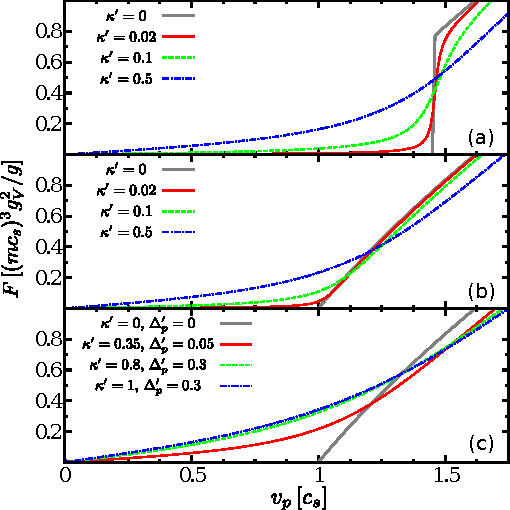
\includegraphics[width=0.6\linewidth]{dragspeed} % ~/ownCloud/documents/phd_projects/point_defect_1_fluid/paper/plots/dragspeed
\caption{
%
Drag force $F$ as a function of the fluid velocity
$v_p$ for different values of the pump detuning $\Delta_p$:
$\Delta_p=-0.3g|\Psi_0|^2$ (a), $\Delta_p=0$ (b), and $\Delta_p>0$
(c), and for different values of the polariton lifetime --- here, we
use the notation $\kappa' = \kappa/g|\psi_0|^2$ and $\Delta_p' =
\Delta/g|\psi_0|^2$.
%
}\label{fig:dragv}
\end{figure}
%
%
\begin{figure}[tb]\centering
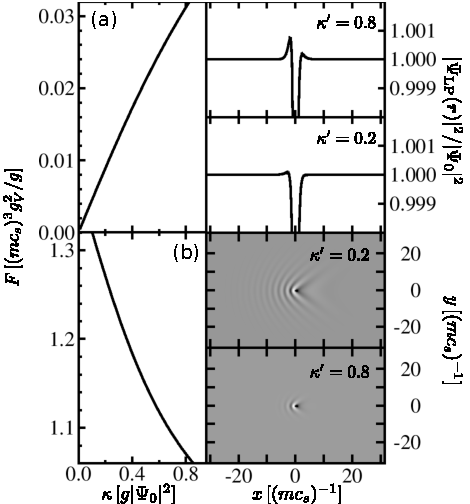
\includegraphics[width=0.6\linewidth]{dragkappa} % ~/ownCloud/documents/phd_projects/point_defect_1_fluid/paper/plots/kappa
\caption{
%
Drag force $F$ as a function of the inverse polariton
lifetime $\kappa'=\kappa/(g |\psi_0|^2)$ in the (a) subcritical regime
($v_p=0.2 c_s$) and (b) supercritical regime ($v_p=1.9 c_s$). In both
cases we have fixed $\Delta_p=-0.3g|\Psi_0|^2$ ($v^c \simeq 1.46 c_s$)
but these results are qualitatively similar for any other value of the
pump detuning. We plot in the insets the normalised real-space
wavefunction $|\psi_{LP}(\bm{r})|^2/|\psi_0|^2$ for two specific
values of $\kappa'=0.2$ and $\kappa'=0.8$.
%
}\label{fig:dragk}
\end{figure}
%


\section{Drag force}
\label{sec:drag}
%
The steady state response of the system to a static and weak defect
can be evaluated starting from Eq.~\eqref{eq:linre}:
%
\begin{equation*}
  \begin{pmatrix} \delta \psi_s(\bm{r}) \\ \delta
    \psi_s^*(\bm{r}) \end{pmatrix} =
  \hat{\mathcal{L}}^{-1} \begin{pmatrix} V(\bm{r}) e^{i \bm{k}_p
      \cdot \bm{r}} \psi_0 \\ -V(\bm{r}) e^{-i \bm{k}_p \cdot
      \bm{r}} \psi_0^{\star} \end{pmatrix} \; .
\end{equation*}
%
For a point-like defect, this can be written in momentum space as:
%
\begin{equation*}
  \delta \psi_s (\bm{k} + \bm{k}_p) = \frac{-g_V \psi_0
    (\varepsilon(\bm{k}) - \bm{k} \cdot \bm{v}_p +
    i\kappa)}{\varepsilon(\bm{k}) [\varepsilon(\bm{k}) +
      2g|\psi_0|^2] - (\bm{k} \cdot \bm{v}_p - i\kappa)^2} \; ,
\end{equation*}
%
while the other component $\delta \psi_s^* (\bm{k}_p - \bm{k})$
can be obtained by complex conjugation and by substituting $\bm{k}
\mapsto -\bm{k}$. The drag force exerted by the defect on the fluid
is given by~\cite{Astrakharchik_2004}:
%
\begin{equation}
  \bm{F} = - \int d\bm{r} |\psi_{LP}(\bm{r},t)|^2 \bm{\nabla}
  (V(\bm{r})) \; ,
\end{equation}
%
and, in the steady state linear response regime, we obtain:
%
\begin{multline}
  \bm{F} = g_V \int \frac{d\bm{k}}{(2\pi)^2} i\bm{k}
  \left[\psi_0^* \delta\psi_s (\bm{k} + \bm{k}_p) + \psi_0 \delta
    \psi_s^* (\bm{k}_p - \bm{k})\right]\\
%
  = 2g_V^2|\psi_0|^2 \int \frac{d\bm{k}}{(2\pi)^2} \frac{i\bm{k}
    \varepsilon(\bm{k})}{\omega^{+} (\bm{k})\omega^{-} (\bm{k})}
  \; .
    \label{eq:dragf}
\end{multline}
%
The drag is clearly oriented along the fluid velocity $\bm{v}_p$,
i.e., $\bm{F} = F \hat{\bm{v}}_p$. If $\kappa \to 0$, then the
integral in Eq.~\eqref{eq:dragf} is finite only if poles exist when
$\Re [\omega^{\pm} (\bm{k})] = 0$, i.e., when quasiparticles can be
excited, in agreement with the Landau criterion. For finite polariton
lifetimes, however, it is clear that the integral will always be
different from zero for $v_p>0$.
% Note that the only dependence on the polariton lifetime $\kappa$ is
%in the denominator of the integral in Eq.~\eqref{eq:dragf}.
We now analyse the behaviour of the drag force as a function of the
fluid velocity for the three ($\Delta_p = 0$, $\Delta_P > 0$, and
$\Delta_p < 0$) different spectra illustrated in the previous section.

For the \emph{linear} spectrum, at $\Delta_p=0$, in the equilibrium
limit, $\kappa \to 0$, we recover for the drag the known result of
weakly interacting Bose gases in two
dimensions~\cite{Astrakharchik_2004}:
%
\begin{equation}
  \frac{F}{(mc_s)^3 g_V^2/g}=\frac{(v_p/c_s)^2 - 1}{v_p/c_s}
  \Theta(v_p - c_s)\; ,
\label{eq:drag0}
\end{equation}
%
with a threshold-like behaviour at a critical fluid velocity equal to
the speed of sound $c_s$. This limiting result is plotted as a bold
gray line in the panels (b,c) of Fig.~\ref{fig:dragv}. For
$\Delta_p=0$ and finite lifetimes $\kappa$, we find a smooth crossover
from the subsonic to the supersonic regime, with the drag being closer
to the equilibrium threshold behaviour for decreasing $\kappa$ (see
Fig.~\ref{fig:dragv}(b)). A finite lifetime tends to increase the
value of the drag in the subsonic region $v_p \ll v^c$, giving place
to a residual drag force, similar to what was found in the numerical
simulations of Ref.~\cite{Cancellieri_2010}. Instead, in the supersonic
region $v_p \gg v^c$, the finite lifetime tends to decrease the value
of the drag. In the case of \emph{diffusive-like} spectra at
$\Delta_p>0$ the situation is qualitatively very similar to the
resonant case (see Fig.~\ref{fig:dragv}(c)), with the difference that
now, in order to have stable solutions, we can decrease the value of
the lifetime only by decreasing accordingly also the value of the pump
detuning $\Delta_p$. The crossover for both $\Delta_p = 0$ and
$\Delta_p > 0$ is also qualitatively very similar to the case of
non-resonantly pumped polaritons~\cite{Wouters_2010}, where the
spectrum of excitation is diffusive-like.

In the case of \emph{gapped} spectra, the situation is, however,
qualitatively different (see Fig.~\ref{fig:dragv}(a)). For infinitely
living polaritons, $\kappa \to 0$, the drag force can also be
evaluated analytically and its expression is similar to
Eq.~\eqref{eq:drag0}, but with a critical velocity larger than the
speed of sound, which expression is given in Eq.~\eqref{eq:criti}:
%
\begin{equation}
  \frac{F}{(mc_s)^3 g_V^2/g}=\frac{(v_p/c_s)^2 - 1}{v_p/c_s}
  \Theta(v_p - v^c)\; .
\end{equation}
%
Therefore now the drag experiences a jump for $v_p=v^c$, rather than a
continuous threshold as for the resonant case $\Delta_p=0$. As already
mentioned in the previous section, this discontinuous behaviour of the
drag for the gapped spectra is connected to the fact that, as soon as
quasiparticles can be excited by the defect at $v_p\ge v^c$,
Cherenkov-like waves can be immediately emitted in all directions,
rather than being restricted in a region outside the Mach cone as
before. For $\Delta_p=0$, the cone was gradually closing with
increasing  fluid velocity.

Both the increase of the value of the drag in the subcritical region
as a function of the polariton lifetime and the decrease in the
supercritical region, are behaviours common to all the types of
spectra. We plot the drag force as a function of $\kappa$ in
Fig.~\ref{fig:dragk}, for two values of the fluid velocity $v_p$ and a
specific value of the pump detuning $\Delta_p$, though we have checked
that the following results are generic. For $v_p < v^c$, we find that
the residual drag is a finite-lifetime effect only, and, in agreement
with the results of Ref.~\cite{Cancellieri_2010}, we find that, well
below the critical velocity, the drag force goes linearly to zero for
$\kappa \to 0$. In the resonant case $\Delta_p=0$, the slope of the
drag for $v_p \ll c_s$ can be evaluated analytically starting from the
expression~\eqref{eq:dragf}:
%
\begin{equation*}
    \frac{F}{(mc_s)^3 g_V^2/g} \mathop{\simeq}\limits_{\kappa \to 0} \frac{2 c_s}{\pi
      v_p} \left( \frac{1}{ \sqrt{1-(v_p/c_s)^2}} - 1 \right)
    \frac{\kappa}{g |\psi_0|^2} \; .
\end{equation*}
%
The residual drag in the subsonic regime is an effect of the
broadening of the quasi-particles energies: Even when the spectrum
real part does not allow any scattering against the defect (e.g., for
$\Delta_p \le 0$), the broadening produces some scattering close to
the defect. This results in a perturbation of the fluid around the
defect, asymmetric in the direction of the fluid velocity (see panel
(a) of Fig.~\ref{fig:dragk}), similar to what  was obtained in
Ref.~\cite{Cancellieri_2010}. Instead, in the supersonic regime, the
drag force is weaker in the non-equilibrium case with respect to the
equilibrium one. This is caused by the finite lifetime tending to
suppress the propagation of the Cherenkov waves away from the defect,
as shown in panel (b) of Fig.~\ref{fig:dragk}.




\section{Conclusions and discussion}
\label{sec:concl}
%
To conclude, we have analysed the linear response to a weak defect of
resonantly pumped polaritons in the pump-only state, and we have been
able to determine two different kinds of threshold like behaviours for
the drag force as a function of the fluid velocity. In the case of
either zero or positive pump detuning, one can continuously connect to
the case of equilibrium weakly interacting gases, where the drag
displays a continuous threshold with a critical velocity equal to the
speed of sound. However, for negative pump detuning, where the
spectrum of excitations is gapped, the drag shows a discontinuity with
a critical velocity larger than the speed of sound. In this sense, the
case of coherently driven microcavity polaritons in the pump-only
configuration displays a richer phenomenology than the case of
polariton superfluids non resonantly pumped. It would be interesting
to perform a similar analysis in the case of polaritons in the optical
parametric oscillator regime, where polaritons are parametrically
scattered from the pump state to the signal and idler states. Here,
the spectrum of excitations has been already determined in
Ref.~\cite{Wouters_2007}, however it is far from clear what are the
conditions for subcritical, superfluid, behaviour in a fluid
characterised by three distinct currents, and how the link between
signal and idler imposed by the parametric scattering influences the
scattering of both fluids against a defect.


\begin{subappendices}
\section{Gross-Pitaevskii equation for the LP field}
\label{app:full}
%
% TODO: make link to formulas in Chapter 3
If one starts from a descriptions of polaritons in terms of separate
exciton and cavity photon fields, a rotation into the lower and upper
polariton basis, followed by neglecting the occupancy of the upper
polariton branch, results in the following Gross-Pitaevskii equation
for the LP field in momentum space
$\psi_{LP}(\bm{r},t) = \sum_{\bm{k}} e^{i\bm{k}\cdot \bm{r}}
\psi_{LP,\bm{k}} (t)$~\cite{Ciuti_2003}:
%
\begin{multline}
  i\partial_t \psi_{LP,\bm{k}} = f_p e^{-i\omega_p t}
  \delta_{\bm{k},\bm{k}_p} + \left[\omega_{LP} (k) - i\kappa
    (k)\right]\psi_{LP,\bm{k}} +\\
%
  \sum_{\bm{k}_1, \bm{k}_2} g_{\bm{k}, \bm{k}_1, \bm{k}_2}
  \psi^*_{LP,\bm{k}_1 + \bm{k}_2-\bm{k}} \psi_{LP,\bm{k}_1}
  \psi_{LP,\bm{k}_2} +\\ s_k \sum_{\bm{k}_1} V_{\bm{k} -
    \bm{k}_1} \psi_{LP,\bm{k}_1} s_{k_1}\; ,
\end{multline}
%
where $\kappa(k)=\kappa_X c^2_k + \kappa_C s^2_k$ is the effective LP
decay rate,
%
\begin{equation}
  g_{\bm{k}, \bm{k}_1, \bm{k}_2}=g_X c_{k}c_{|\bm{k}_1 + \bm{k}_2-\bm{k}|} c_{k_1} c_{k_2}
\end{equation}
%
is the interaction strength, and where
$V(\bm{r}) = \sum_{\bm{k}} e^{i\bm{k}\cdot \bm{r}} V_{\bm{k}}$.

In these expressions, the coefficients
%
\begin{equation}
  c^2_{k}, s^2_{k} = \frac{1}{2} \left(1 \pm \frac{\omega_C(k) -
    \omega_X^0}{\sqrt{(\omega_C(k) - \omega_X^0)^2 +
      \Omega_R^2}}\right)
\end{equation}
%
are the Hopfield coefficients used to diagonalise the free polariton
Hamiltonian. We want here to justify the simplified description done
in Eq.~\eqref{eq:basic}. If we follow the linear response expansion as
in~\eqref{eq:mfield}, the operator $\hat{\mathcal{L}}$ in momentum
space analogous to~\eqref{eq:opell} reads as:

%
\begin{equation}
  \mathcal{L}_{\bm{k},\bm{k}_p} = \begin{pmatrix}
    \widetilde{\omega_{LP}} (\delta \bm{k}+\bm{k}_p) - i
    \kappa(\delta \bm{k}+\bm{k}_p) & g_X c_{k_p}^2 c_{\delta
      \bm{k}+\bm{k}_p} c_{\delta \bm{k}-\bm{k}_p} \psi_0^2
    \\ - g_X c_{k_p}^2 c_{\delta \bm{k}+\bm{k}_p} c_{\delta
      \bm{k}-\bm{k}_p}{\psi_0^{\star}}^2 & -
    \widetilde{\omega_{LP}}(\delta \bm{k}-\bm{k}_p) -
    i\kappa(\delta \bm{k}-\bm{k}_p) \end{pmatrix}\; ,
\label{eq:opel2}
\end{equation}
%

where now $\widetilde{\omega_{LP}} (\delta \bm{k} \pm\bm{k}_p) =
\omega_{LP} (\delta \bm{k} \pm\bm{k}_p) -\omega_p + 2 g_X
c_{k_p}^2 c_{\delta \bm{k} \pm \bm{k}_p}^2 |\psi_0|^2$. It is easy
to show that the eigenvalues of this operator coincide with our
approximated expressions~\eqref{eq:spect} in the limit of $\delta k
\ll k_p$, when $c_{\delta \bm{k} \pm \bm{k}_p}^2 \simeq
c_{k_p}^2$, $s_{\delta \bm{k} \pm \bm{k}_p}^2 \simeq s_{k_p}^2$
and when we can simply rename $g=g_X c_{k_p}^4$ and $\kappa =
\kappa(k_p)$. It is interesting to note that, even if we would retain
the linear terms in $\bm{k}_p \cdot \delta \bm{k}$ in the
expansion of $c_{\delta \bm{k} \pm \bm{k}_p}^2$, this would result
in a renormalisation of the fluid velocity $\bm{v}_p$ in the
expression~\eqref{eq:spect} which takes into account the blue-shift of
the lower polariton dispersion due to the interaction.

\end{subappendices}

% TODO: cite Larr__2012 (1D case)
% TODO: include residual drag figure from Cancellieri_2010
% TODO: cite Van_Regemortel_2014 (negative drag)
% TODO: Amo_2009 -- include pic; fig. 2&20 QFL

%%% Local Variables:
%%% mode: latex
%%% TeX-master: "../thesis_berceanu"
%%% End:

\chapter{On multicomponent polariton superfluidity in the optical
  parametric oscillator regime}
\label{cha:opo}

%TODO%
%%%%%%%%%%%%%%%%%%%%%%%%%%%%%%%%%%%%%%%%%%%%%%%%%%%%%%%%%%%%%%%%%%%%%%%
% As no restoring force opposes a global rotation of the signal-idler %
% phases, the generator of such rotations is an eigenvector of L with %
% eigenvalue 0.                                                       %
%%%%%%%%%%%%%%%%%%%%%%%%%%%%%%%%%%%%%%%%%%%%%%%%%%%%%%%%%%%%%%%%%%%%%%%

\section{Introduction}
%
Microcavity polaritons, the novel quasiparticles resulting from the
coherent strong coupling between quantum well excitons and cavity
photons~\cite{9780199228942}, have unique mixed matter-light
properties that none of their constituents displays on its
own. Because of their energy dispersion and their strong non-linearity
inherited from the excitonic components, polaritons continuously
injected by an external laser into a pump state with suitable
wavevector and energy can undergo coherent stimulated scattering into
two conjugate states~\cite{Ciuti_2000,Ciuti_2001,Ciuti_2003}, the signal
and the idler, a process known as optical parametric oscillator (OPO).
%
Since their first
realisation~\cite{Stevenson_2000,Savvidis_2000,Savvidis_2000_b,Baumberg_2000,Saba_2001},
the interest in microcavity optical parametric phenomena has involved
several fields of fundamental and applicative
research~\cite{Edamatsu_2004,Savasta_2005,Lanco_2006,Abbarchi_2011,Ardizzone_2012,Xie_2012,Lecomte_2013}.

Recently, considerable resources have been invested in exploring the
fundamental properties of parametric processes, including the
possibility of macroscopic phase coherence and superfluid
behaviour~\cite{Carusotto_2013}.
%
In spite of the coherent nature of the driving laser pump, the OPO
process belongs to the class of non-equilibrium phase transitions, in
which a $U(1)$ phase symmetry is spontaneously
broken~\cite{Wouters_2007}.
%
While the phase of the pumped mode is locked to the incident laser,
the ones of signal and idler are free to be simultaneously rotated in
opposite directions.
%
Because of this phase freedom, recent experiments~\cite{Sanvitto_2010}
have tested the OPO superfluid properties by exploring the physics of
the signal-idler order parameter, demonstrating the existence and
metastability of vortex configurations. As the order parameter
involves both signal and idler, their phase winding have opposite
signs~\cite{Sanvitto_2010,Marchetti_2010,9783642241857}.  Crucially, this
makes both OPO fluids to display quantized flow metastability
simultaneously.

While in equilibrium condensates different aspects of superfluidity
are typically closely related~\cite{Leggett_1999}, this is no longer
true in a non-equilibrium context as for microcavity
polaritons~\cite{Carusotto_2013}.
%
In particular, those aspects of superfluidity related to the
frictionless flow around defects are expected to be much more involved
in OPO condensates than for any other investigated polariton
condensates, such as for the case of incoherent
pumping~\cite{Kasprzak_2006,Wouters_2010}, and single-state
resonantly pumped microcavities~\cite{Amo_2009}.
%
Independently on the pumping scheme, the driving and the polariton
finite lifetime prompt questions about the meaning of superfluid
behaviour, when the spectrum of collective excitations is complex
rather than real, raising conceptual interrogatives about the
applicability of a Landau criterion~\cite{Wouters_2010}.
%
Yet, an additional complexity characterises the OPO regime, where the
simultaneous presence of three oscillation frequencies and momenta for
pump, signal and idler correspondingly multiplies the number of
collective excitation branches~\cite{Wouters_2007}.
%
Note that from the experimental point of view, pioneering
experiments~\cite{Amo_2009_b} have observed a ballistic non-spreading
propagation of signal/idler polariton wavepackets in a triggered-OPO
configuration.
%
However, given the complexity of the dynamics as well as the nonlinear
interactions involved in this time-dependent
configuration~\cite{Szyma_ska_2010}, theoretical understanding of these
observations is not complete yet.

% Account of results.
This Article reports a joint theoretical and experimental study of an
OPO configuration where a wide and steady-state condensate hits a
stationary localised defect in the microcavity.
%
Contrary to the criterion for quantized flow metastability for which
signal and idler display simultaneous locked responses, we find that
their scattering properties when the OPO hits a static defect are
different.
%
In particular we investigate the scattering properties of all three
fluids, pump, signal and idler, in both real and momentum space. We
find that the modulations generated by the defect in each fluid are
determined not only by its associated Rayleigh scattering ring, but
each component displays additional rings because of the cross-talk
with the other components imposed by nonlinear and parametric
processes.
%
We single out three factors determining which one of these rings
influences the most each fluid response: the coupling strength between
the three OPO states, the resonance of the ring with the blue-shifted
lower polariton dispersion, the values of each fluid group velocity
and lifetime together establishing how far each modulation can
propagate from the defect.
%
The concurrence of these effects implies that the idler strongly
scatters inheriting the same modulations as the pump, while the
modulations due to its own ring can propagate only very close to the
defect and cannot be appreciated. Yet, the modulations in the signal
are strongly suppressed, and not at all visible in experiments,
because the slope of the polariton dispersion in its low momentum
component brings all Rayleigh rings coming from pump and idler out of
resonance.

Note that the kinematic conditions for OPO are incompatible with the
pump and idler being in the subsonic regime. Thus, the coupling
between the three components always implies some degree of scattering
in the signal. In practice, the small value of the signal momentum
strongly suppresses its actually visible modulations, something
confirmed by the experimental observations.


%
\begin{figure}[tb]
\centering
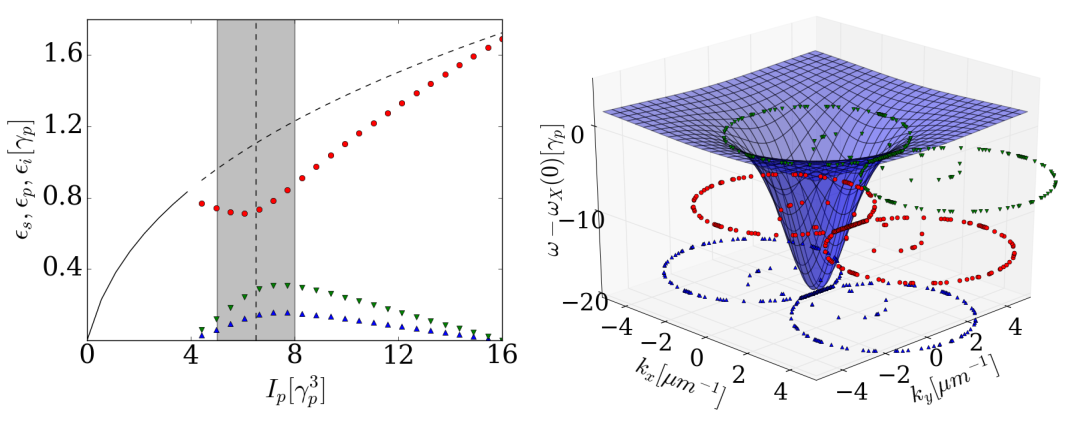
\includegraphics[width=.5\linewidth]{3d0_0} % ~/notebooks/OPODrag/opodrag.py
\caption{OPO mean-field blue-shifts and fluctuation
  Rayleigh rings in the linear response scheme for homogeneous
  pumping. Left panel: Signal $s$ ([blue] upper triangles), pump $p$
  ([red] circles), and idler $i$ ([green] lower triangles) mean-field
  energy blue-shifts $\epsilon_{n=s,p,i}$ (in units of $\gamma_p =
  \gamma_{\vt{k}_p}$) versus the rescaled pump intensity $I_p$ (in
  units of $\gamma_p^3$) in the optical limiter regime. Parameters are
  $\Omega_R=5$~meV, zero cavity-exciton detuning, $\gamma_X = \gamma_C
  = 0.12$~meV, $\omega_p - \omega_0^X = -1.25$~meV, $k_p=1.6{\mu
    m}^{-1}$, $k_s \simeq 0$, and $k_i=3.2{\mu m}^{-1}$.  The shaded
  area is stable OPO region, while the vertical dashed line
  corresponds to the pump power value chosen for plotting the right
  panel. Right panel: Blue-shifted LP dispersion~\eqref{eq:blues} with
  superimposed Rayleigh curves $\Gamma_{p,i,(u,v), \tilde{\vt{k}} +
    \vt{k}_{p, i}}$ evaluated within the linear response
  approximation (same symbols as left panel). The two rings
  corresponding to the signal state, $\Gamma_{s,(u,v),
    \tilde{\vt{k}}}$, are shrinked to zero because $k_s \simeq 0$.}
\label{fig:spect}
\end{figure}
%
%%%%%%%%%%%%%%%%%%%%%%%%%%%%%%%%%%%%%%%%%%%%%%%%%
\section{Model}
%
The dynamics of polaritons in the OPO regime, and their hydrodynamic
properties when scattering against a defect, can be described via a
classical driven-dissipative non-linear Gross-Pitaevskii equation
(GPE) for the coupled exciton and cavity fields $\psi_{X,C}
(\vt{r},t)$ ($\hbar=1$)~\cite{Whittaker_2005,Carusotto_2013}:
%
\begin{equation}
  i\partial_t \begin{pmatrix} \psi_X \\ \psi_C \end{pmatrix} =
  \hat{H} \begin{pmatrix} \psi_X \\ \psi_C \end{pmatrix}
  + \begin{pmatrix} 0 \\ F_p(\vt{r},t) \end{pmatrix} \; .
\label{eq:gpequ}
\end{equation}
%
The dispersive $X$- and $C$-fields decay at a rate $\gamma_{X,C}$ and
are coupled by the Rabi splitting $\Omega_R$, while the non-linearity
is regulated by the exciton coupling strength $g_X$:
%
\begin{equation}
  \hat{H} = \begin{pmatrix} \omega^{X}_{-i\nabla} - i
    \frac{\gamma_X}{2} + g_X |\psi_X|^2 & \Omega_R/2 \\ \Omega_R/2 &
    \omega^C_{-i\nabla} - i \frac{\gamma_C}{2} + V_d \end{pmatrix} \;
  .
\end{equation}
%
We describe the defect via a potential $V_d (\vt{r})$ acting on the
photonic component; this can either be a defect in the cavity mirror
or a localised laser field~\cite{Amo_2009,Amo_2010,Zajac_2012}.
%
In the conservative, homogeneous, and linear regime ($\gamma_{X,C}=0=
V_d (\vt{r})= g_X$), the eigenvalues of $\hat{H}$ are given by the
lower (LP) and upper polariton (UP) energies, $2
\omega_{\vt{k}}^{LP,UP} = \omega_{\vt{k}}^{C} +
\omega_{\vt{k}}^{X} \mp \sqrt{(\omega_{\vt{k}}^{C} -
  \omega_{\vt{k}}^{X})^2 + \Omega_R^2}$.
%
The cavity is driven by a continuous-wave laser field $F_p(\vt{r},t)
= \mathcal{F}_p(\vt{r}) e^{i (\vt{k}_p \cdot \vt{r} - \omega_p
  t)}$ into the OPO regime: Here, polaritons are continuously injected
into the pump state with frequency $\omega_p$ and momentum
$\vt{k}_p$ and, above a pump strength threshold, undergo coherent
stimulated scattering into the signal $(\omega_s, \vt{k}_s)$ and
idler $(\omega_i, \vt{k}_i)$ states. 

As a first step, it is useful to get insight into the system behaviour
in the simple case of a homogeneous pump of strength
$\mathcal{F}_p(\vt{r}) = f_p$. A numerical study of the coupled
equations~\eqref{eq:gpequ} for the more realistic case of a
finite-size top-hat pump profile $\mathcal{F}_p(\vt{r})$ will be
presented later.
%
To further simplify our analysis, we assume here that the UP
dispersion does not get populated by parametric scattering processes
and thus, by means of the Hopfield coefficients $2X_{\vt{k}}^2,
2C_{\vt{k}}^2 = 1 \pm (\omega_{\vt{k}}^{C} -
\omega_{\vt{k}}^{X})/\sqrt{(\omega_{\vt{k}}^{C} -
  \omega_{\vt{k}}^{X})^2 + \Omega_R^2}$, we project the
GPE~\eqref{eq:gpequ} onto the LP
component~\cite{Ciuti_2001,Wouters_2007_b} $\psi_{\vt{k}}^{} =
X_{\vt{k}} \psi_{X,\vt{k}} + C_{\vt{k}} \psi_{C,\vt{k}}$,
where $\psi(\vt{r},t) = \sum_{\vt{k}} e^{i\vt{k}\cdot \vt{r}}
\psi_{\vt{k}}^{} (t)$:
%
\begin{multline}
  i\partial_t \psi_{\vt{k}}^{} = \left[\omega_{\vt{k}}^{LP} -
    i\frac{\gamma_{\vt{k}}}{2}\right]\psi_{\vt{k}}^{} +
  C_{\vt{k}} \sum_{\vt{q}} C_{\vt{q}} V_d(\vt{k} - \vt{q})
  \psi_{\vt{q}}^{}\\ + \sum_{\vt{k}_1, \vt{k}_2} g_{\vt{k},
    \vt{k}_1, \vt{k}_2} \psi^*_{\vt{k}_1 + \vt{k}_2-\vt{k}}
  \psi_{\vt{k}_1}^{} \psi_{\vt{k}_2}^{} + \tilde{f}_p(t)
  \delta_{\vt{k},\vt{k}_p}\; .
\label{eq:efflp}
\end{multline}
%
Here, $\gamma_{\vt{k}}=\gamma_X X_{\vt{k}}^2 + \gamma_C
C_{\vt{k}}^2$ is the effective LP decay rate, the interaction
strength is given by $g_{\vt{k}, \vt{k}_1, \vt{k}_2}=g_X
X_{\vt{k}} X_{\vt{k}_1 + \vt{k}_2-\vt{k}} X_{\vt{k}_1}
X_{\vt{k}_2}$, and the pumping term by $\tilde{f}_p(t)=
C_{\vt{k}_p} f_p e^{-i\omega_p t}$.


%%%%%%%%%%%%%%%%%%%%%%%%%%%%%%%%%%%%%%%%%%%%%%%%%
\section{Linear response theory}
%
In the limit where the homogeneously pumped system is only weakly
perturbed by the external potential $V_d(\vt{r})$, we apply a linear
response analysis~\cite{Astrakharchik_2004}: The LP field is expanded
around the mean-field terms for the three $n=1,2,3=s,p,i$ OPO
states~\cite{Whittaker_2005},
%
\begin{equation}
  \psi_{\tilde{\vt{k}}}^{} = \sum_{n=1}^3 e^{-i \omega_n t}
  \left[\psi_{n}^{} \delta_{\tilde{\vt{k}},0} +
    u_{n,\tilde{\vt{k}}}^{} e^{-i\omega t} +
    v^*_{n,-\tilde{\vt{k}}} e^{i\omega t} \right]\; ,
\label{eq:expan}
\end{equation}
%
where $\tilde{\vt{k}} = \vt{k} - \vt{k}_n$. Eq.~\eqref{eq:efflp}
is expanded linearly in both the fluctuations terms,
$u_{n,\tilde{\vt{k}}}^{}$ and $v_{n,\tilde{\vt{k}}}^{}$, as well
as the defect potential.  At zero-th order, the three complex uniform
mean-field equations can be solved to obtain the dependence of the
signal, pump and idler energy blue-shifts, $\epsilon_n = g_X
X^2_{\vt{k}_n} |\psi_{n}^{}|^2$ on the system
parameters~\cite{Wouters_2007_b,SM}. A typical behaviour of
$\epsilon_n$ as a function of the rescaled pump intensity $I_p = g_X
C_{\vt{k}_p}^2 f_p^2/X_{\vt{k}_p}^2$ in the optical limiter regime
is plotted in the left panel of Fig.~\ref{fig:spect}.
%
At first order, one obtains six coupled equations diagonal in momentum
space~\cite{Wouters_2007}
%
\begin{equation}
  \omega \vt{w}_{\tilde{\vt{k}}} = \mathcal{L}_{\tilde{\vt{k}}}
  \vt{w}_{\tilde{\vt{k}}} + \frac{1}{2} \bm{\Psi}_d\; ,
\label{eq:fluct}
\end{equation}
%
for the $6$-component vector $\vt{w}_{\tilde{\vt{k}}} =
(u_{n,\tilde{\vt{k}}}^{} , v_{n,\tilde{\vt{k}}}^{})^{T}$ and for
the potential part, $\bm{\Psi}_d = (\psi_n^{} C_{\vt{k}_n}
C_{\vt{k} + \vt{k}_n} V_d(\vt{k}),-\psi_n^* C_{\vt{k}_n}
C_{\vt{k}_n - \vt{k}} V_d(-\vt{k}))^{T}$. In ~\eqref{eq:fluct}
we have only kept the terms oscillating at the frequencies $\omega_n
\pm \omega$ and neglected the other terms in the expansion (i.e.,
$2\omega_n - \omega_m \pm \omega$), which are oscillating at
frequencies far from the LP band, and thus with negligible amplitudes.
%
In the particle-like and the hole-like channels, the Bogoliubov matrix
determining the spectrum of excitations can be written
as~\cite{Wouters_2007}
%
\begin{equation}
  \mathcal{L}_{\vt{k}} = \begin{pmatrix} M_{\vt{k}}^{} & Q_{\vt{k}}^{}
    \\ -Q_{-\vt{k}}^* & -M_{-\vt{k}}^* \end{pmatrix} \; ,
\end{equation}
%
where the 3 OPO states components are
%
\begin{align}
  (M_{\vt{k}}^{})_{mn} &= \left[\omega^{LP}_{\vt{k}_m + \vt{k}}
    - \omega_m - i\frac{\gamma_{\vt{k}_m + \vt{k}}}{2}\right]
  \delta_{m,n} \\
%
  \nonumber & + 2\sum_{q,t=1}^3
  g_{\vt{k}_m+\vt{k},\vt{k}_n+\vt{k},\vt{k}_t} \psi_q^*
  \psi_t^{} \delta_{m+q,n+t}\\
%
  (Q_{\vt{k}}^{})_{mn} &= \sum_{q,t=1}^3
  g_{\vt{k}_m+\vt{k},\vt{k}_q,\vt{k}_t} \psi_q^{} \psi_t^{}
  \delta_{m+n,q+t}\; .
\end{align}
%


%
\begin{figure}[tb]
\centering
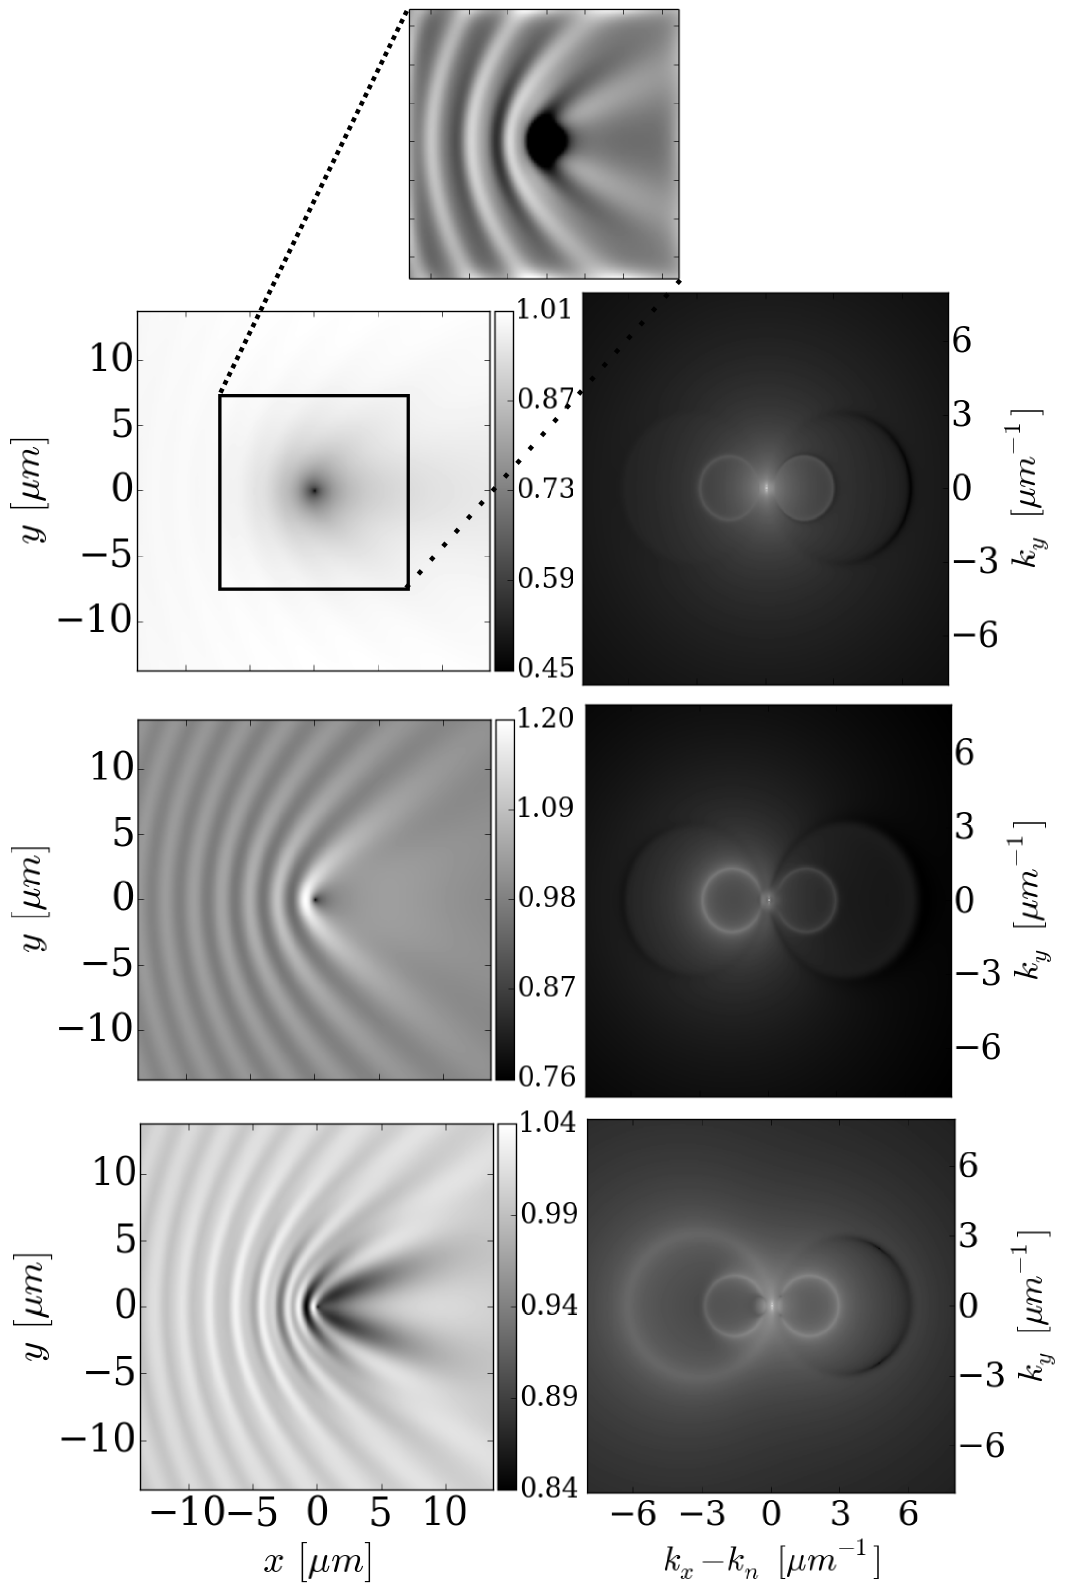
\includegraphics[width=.5\linewidth]{ks0_0}
% ~/notebooks/julia/april/linresp_waves.ipynb
% ~/notebooks/OPODrag/opodrag.py
\caption{Linear responses to a static defect of the three OPO states
  in real and momentum space. Rescaled filtered OPO emissions (signal
  [top panels], pump [middle], and idler [bottom]) in real space
  $|\psi (\vt{r},\omega_n)|^2/|\psi_n|^2$ (left panels in linear
  scale) and momentum space $|\psi_{\tilde{\vt{k}}} (\omega_n)|^2$
  (right panel in logarithmic scale) obtained within the linear
  response approximation. The parameters are the same ones of
  Fig.~\ref{fig:spect}. For the top left panel of the signal emission
  in real space, Gaussian filtering is applied to enhance the short
  wavelength modulations, which amplitudes are otherwise roughly $1\%$
  of the average signal intensity and about a factor of 10 times
  weaker than the modulation amplitudes in the pump fluid.}
\label{fig:ereal}
\end{figure}
%
In absence of a defect potential ($\bm{\Psi}_d =0$),
Eq.~\eqref{eq:fluct} is the eigenvalue equation for the spectrum of
excitations of a homogeneous OPO, i.e.,
$\det(\mathcal{L}_{\tilde{\vt{k}}} - \omega)=0$. The spectrum has 6
branches, $\omega_{n,(u,v),\tilde{\vt{k}}}$, labeled by $n=s,p,i$
and $(u,v)$. Even though these degrees of freedom are mixed together,
at large momenta, one recovers the LP dispersions shifted by the three
states energies and momenta, i.e.,:
%
\begin{equation}
  \lim_{\tilde{k} \gg \sqrt{2m_C \Omega_R}} \omega_{n,(u,v),\tilde{\vt{k}}} = \pm
  (\omega^{LP}_{\vt{k} - \vt{k}_n} - \omega_n)\; ,
\label{eq:large}
\end{equation}
%
where $+$ ($-$) corresponds to the $u$ ($v$) particle- (hole-)like
branch.
%
The OPO solution is stable (shaded area in Fig.~\ref{fig:spect}) as
far as $\Im \omega_{n,(u,v),\tilde{\vt{k}}} < 0$.

The shape of the patterns, or Cherenkov-like waves, resulting from the
elastic scattering of the OPO 3-fluids against the static ($\omega=0$)
defect can be determined starting from the spectrum, and in particular
evaluating the closed curves $\Gamma_{n,(u,v), \tilde{\vt{k}}}$ in
$\vt{k}$-space, or ``Rayleigh rings''~\cite{9783319002651} defined
by condition $\Re \omega_{n,(u,v), \tilde{\vt{k}}} =
0$~\footnote{Even if they do not appear to be relevant here, note that
  the presence of a non-vanishing imaginary part of the excitation
  spectrum $Im\omega_{n,(u,v),\tilde{\vt{k}}}\neq 0$ introduces some
  complications: Even in the absence of any Rayleigh ring, the drag
  force can be non-vanishing and the standard Landau criterion may
  fail identifying a critical velocity~\cite{Wouters_2010}.}.
%
The modulations propagate with a direction
$\hat{\eta}_{n,(u,v),\tilde{\vt{k}}}$ orthogonal to each curve
$\Gamma_{n,(u,v), \tilde{\vt{k}}}$, a pattern wavelength given by
the corresponding $|\tilde{\vt{k}}|$, and a group velocity
$\vt{v}_{n,(u,v),\tilde{\vt{k}}}^{(g)}=\nabla_{\tilde{\vt{k}}}
\Re \omega_{n,(u,v), \tilde{\vt{k}}}$, where
$\xi_{n,(u,v),\tilde{\vt{k}}} =
|\vt{v}_{n,(u,v),\tilde{\vt{k}}}^{(g)} / \Im \omega_{n,(u,v),
  \tilde{\vt{k}}}|$ determines the distance, at any given direction
$\hat{\eta}_{n,(u,v),\tilde{\vt{k}}}$, over which the perturbation
extends away from the defect. For a single fluid under a coherent
pump, the qualitative shape of the modulation pattern generated in the
fluid by the defect is mostly determined by the excitation
spectrum~\cite{Carusotto_2006,Carusotto_2004}.

For OPO, the spectrum of excitation on top of each of the three,
$n=1,2,3$, states (see~\cite{SM}) generates six identical Rayleigh
rings $\Gamma_{n,(u,v), \tilde{\vt{k}}}$ for the 3 states.
%
The Rayleigh rings for the OPO conditions specified in
Fig.~\ref{fig:spect} are clearly visible in the right panels of
Fig.~\ref{fig:ereal}, where we plot the $\vt{k}$-space
photoluminescence filtered at each state energy, i.e.,
$|\psi_{\tilde{\vt{k}}} (\omega_n)|^2= |\psi_{n}^{}
\delta_{\tilde{\vt{k}},0} + u_{n,\tilde{\vt{k}}}^{} +
v^*_{n,-\tilde{\vt{k}}}|^2$.
%
We have here chosen a $\delta$-like defect potential, $V_d(\vt{k}) =
g_d$, but we have however checked that our results do not depend on
its exact shape~\cite{SM}.
%
For the OPO conditions considered here, the signal momentum is at $k_s
\simeq 0$, and thus only four of the six rings are present. The same
rings are also plotted in the right panel of Fig.~\ref{fig:spect},
shifted at each of the three OPO state momentum $\vt{k}_n$,
$\Gamma_{n,(u,v), \tilde{\vt{k}}+\vt{k}_n}$ and energies
$\omega_n$.
%
It is important to note that, even though the three OPO states have
locked responses because the three states display the same spectrum of
excitations, only one of the rings $\Gamma_{n,(u,v),
  \tilde{\vt{k}}+\vt{k}_n}$ is the most resonant at $\omega_n$
with the interaction blue-shifted lower polariton dispersion,
%
\begin{equation}
  \bar{\omega}_{\vt{k}}^{LP} = \omega_{\vt{k}}^{LP} + 2 
  X_{\vt{k}}^2 \sum_{n=1}^3  \epsilon_n\; ,
\label{eq:blues}
\end{equation}
%
where $\epsilon_n = g_X X_{\vt{k}_n}^2 |\psi_n^{}|^2$ are the
mean-field energy blue-shifts (measured in Fig.~\ref{fig:spect} in
units of $\gamma_p = \gamma_{\vt{k}_p}$).  This implies that the
most visible modulation for each fluid should be the most resonant
one, with superimposed weaker modulations coming from the other two
state rings.

In the specific case of Fig.~\ref{fig:spect}, the signal is at $k_s
\simeq 0$ and thus produces no rings in momentum space. The other four
rings are very far from being resonant with the blue-shifted LP
dispersion~\eqref{eq:blues} at $\omega_s$, and thus the signal
displays only an extremely weak modulation coming from the next
closer ring, which is the one associated with the pump state,
$\Gamma_{p,u, \tilde{\vt{k}}+\vt{k}_s}$.
%
We estimate that the signal modulation amplitudes are roughly $1\%$ of
the average signal intensity and about a factor of 10 times weaker
than the modulation amplitudes in the pump fluid.
%
In order to show that the signal has weak modulations coming from
the pump, we apply a Gaussian filter to the real space images (see
inset of the left top panel of Fig.~\ref{fig:ereal}).
%
As explained in more details in~\cite{SM}, Gaussian filtering consists
of subtracting from the original data a copy which has been
convoluted with a Gaussian kernel, thus getting rid of the
long-wavelength modulations.
%
This procedure reveals that indeed the pump imprints its modulation
also into the signal, even though these are extremely weak, thus
leaving the signal basically insensitive to the presence of the
defect.

Pump and idler states are each mostly resonant with their own
rings, i.e., $\Gamma_{p,u, \tilde{\vt{k}}+\vt{k}_p}$ at $\omega_p$
and $\Gamma_{i,u, \tilde{\vt{k}}+\vt{k}_i}$ at $\omega_i$,
respectively. Thus one should then observe two superimposed
modulations in both pump and idler filtered emissions, the stronger
one for each being the most resonant one.
%
However, the modulations associated to the idler only propagate very
close to the defect, at an average distance
$\overline{\xi_{i,u,\tilde{\vt{k}}}} \sim 1.7~\mu$m before getting
damped, and thus are not clearly visible. For the OPO conditions
considered, this is due to the small idler group velocity
$\vt{v}_{i,u,\tilde{\vt{k}}}^{(g)}$, as the dispersion is almost
excitonic at the idler energy.

We can conclude that, for the typical OPO condition with a signal at
$k_s \simeq 0$, considered in Figs.~\ref{fig:spect}
and~\ref{fig:ereal}, the signal fluid does not show modulations and
the extremely weak scattering inherited from the pump state can be
appreciated only after a Gaussian filtering procedure of the image. In
contrast, the idler has a locked response to the one of the pump
state.
%
Note that, for the conditions shown in Fig.~\ref{fig:spect}, as well
as the other cases considered in Ref.~\cite{SM}, the subsonic to
supersonic crossover of the pump-only state~\cite{Amo_2009} happens
well above the region of stability of OPO. Thus it is not possible to
study a case where the pump is already subsonic and at the same time
promotes stimulated scattering.
%%

%
\begin{figure}[tb]\centering
  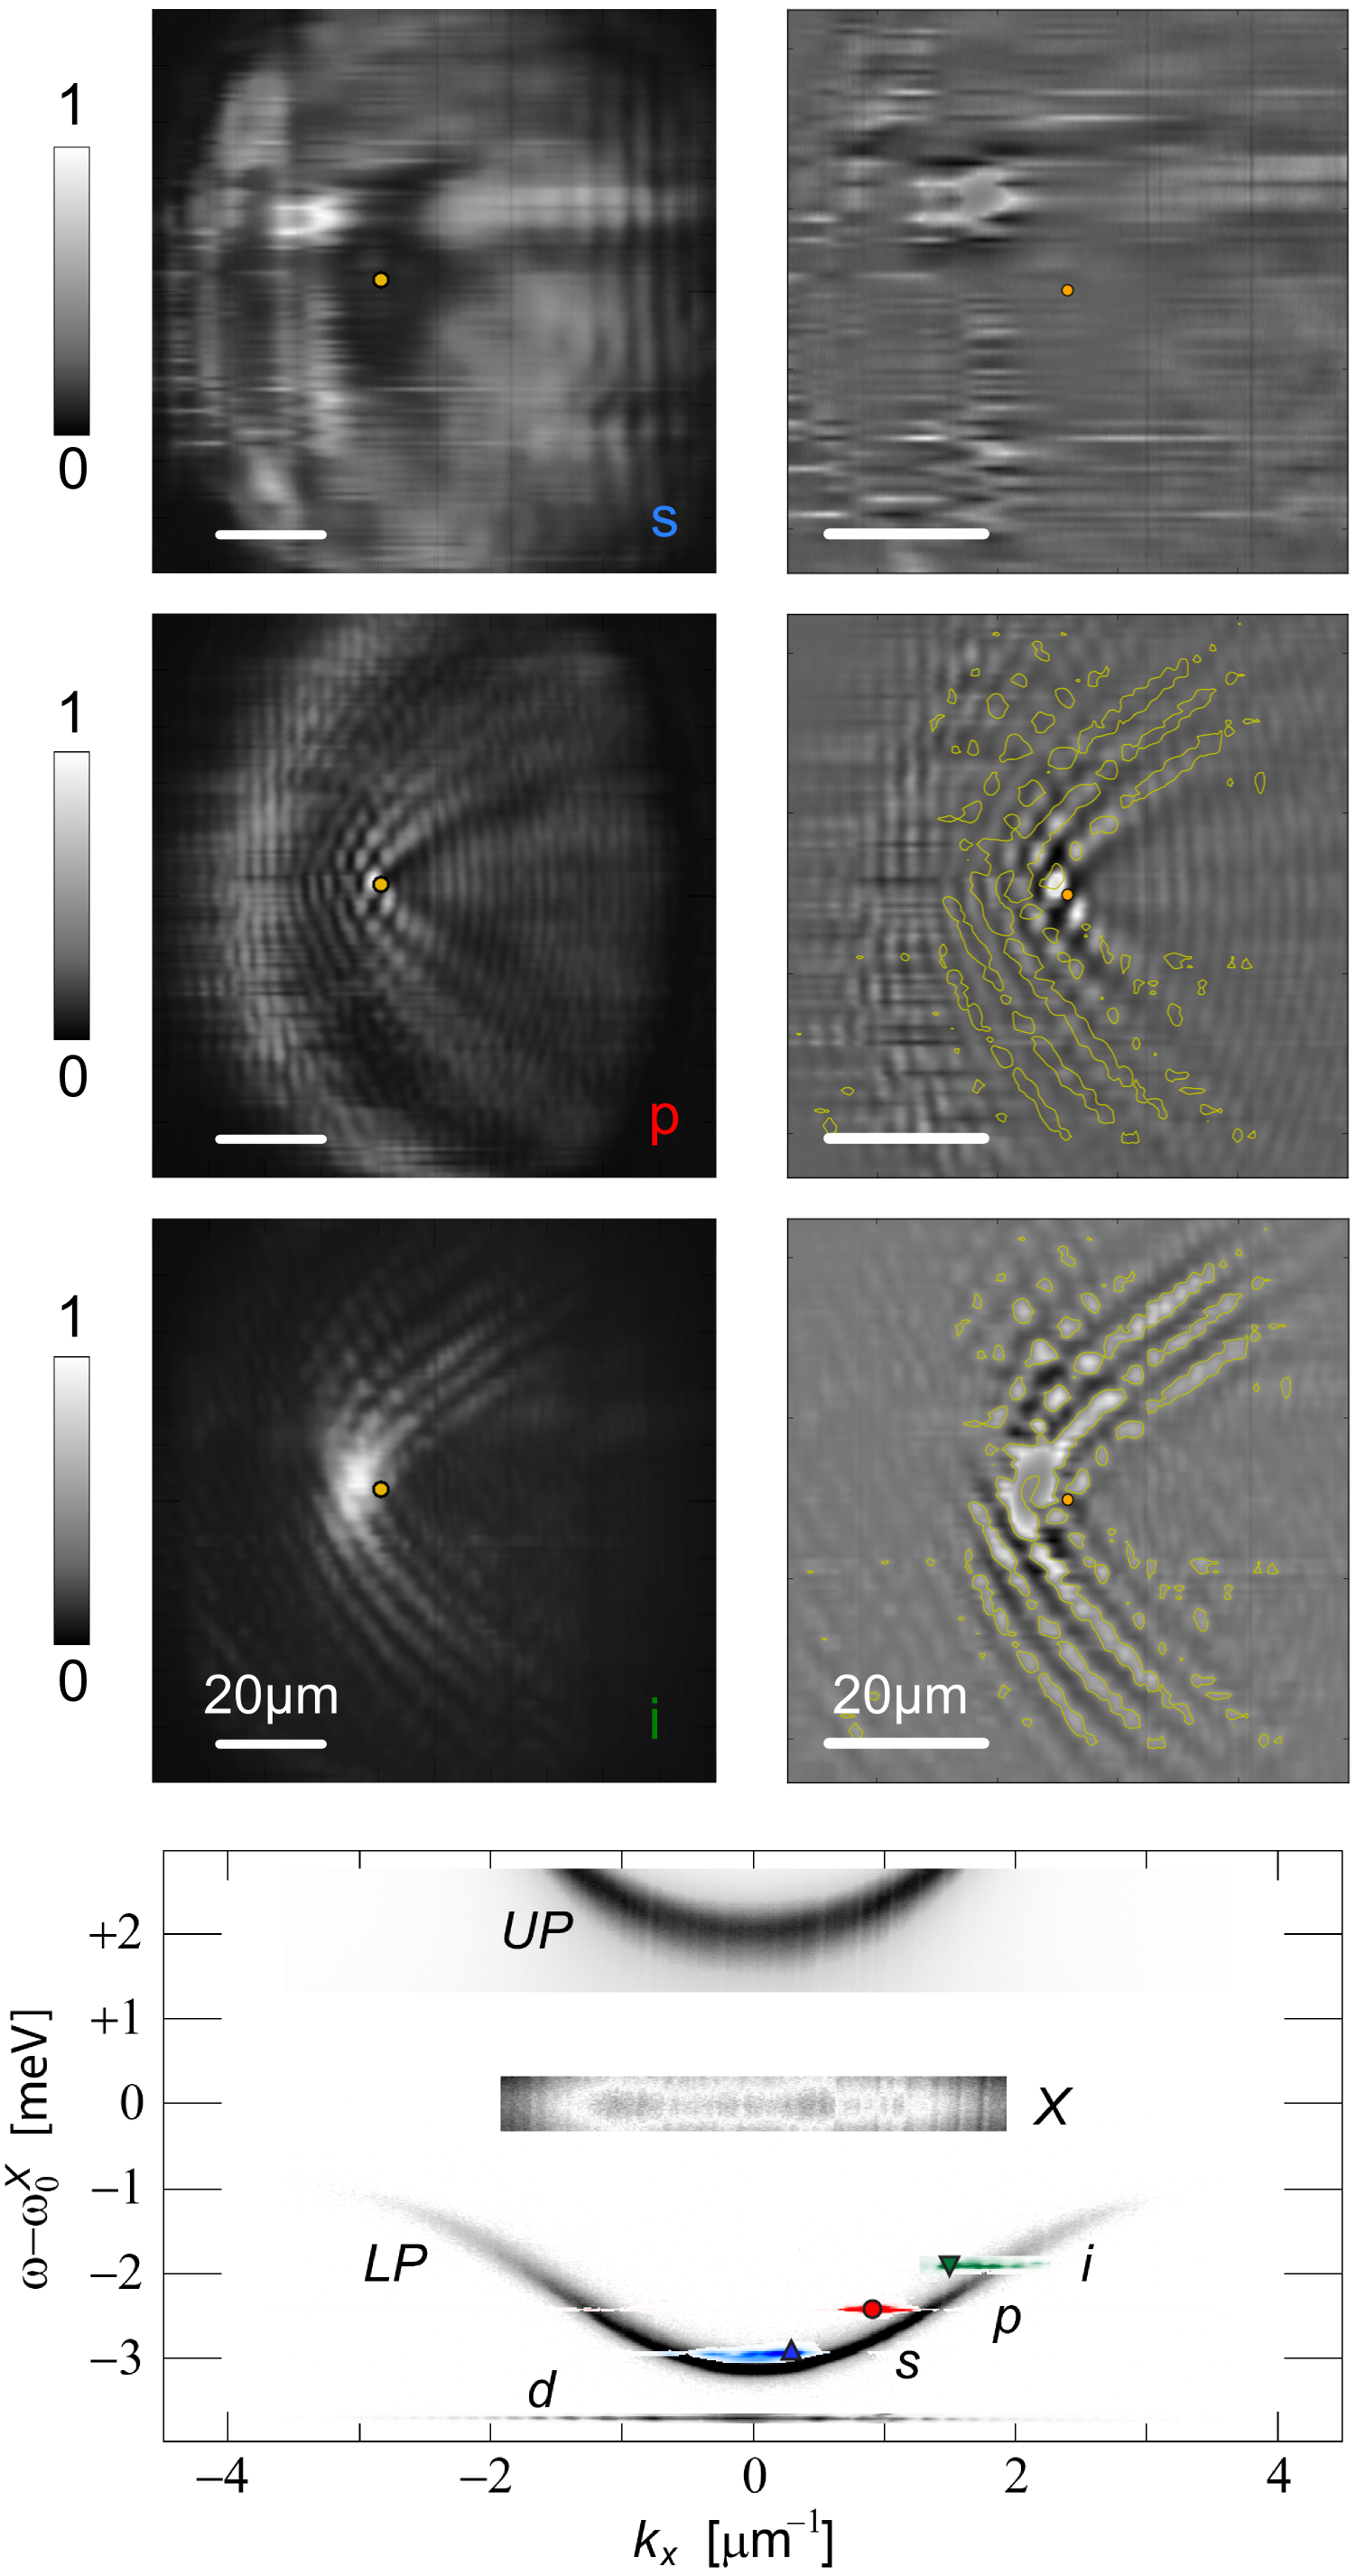
\includegraphics[width=.5\linewidth]{exp_waves}
% ~/notebooks/julia/april/extract_exp_waves.ipynb
\caption{Experimental OPO spectrum and filtered
  emissions of signal, pump and idler in presence of a structural
  defect. The six panels show the filtered emission profiles in real
  space of signal (top), pump (middle) and idler (bottom) $I_{s,
    p,i}(\vt{r})$. A Gaussian filtering to enhance the short
  wavelength modulations is applied in the right column panels. Here,
  the extracted wave-crests from the idler emission (yellow contours
  in the bottom panel) are also superimposed to the pump profile
  (middle) by applying a $\pi$-phase shift. The (orange) dot indicates
  the position of the defect. The lower panel shows the experimental
  OPO spectrum. Energy and momentum of the three OPO states are
  labeled with a [blue] upper triangle (signal), a [red] circle
  (pump), and a [green] lower triangle (idler), while the localised
  state, clearly visible just below the bottom of the LP dispersion,
  is indicated with the symbol $d$. The bare LP dispersion is
  extracted from an off-resonant low pump power measurement, as well
  as the emission of the exciton reservoir (X) and the one of the UP
  dispersion (each in a different scale).}
\label{fig:exper}
\end{figure}
%
%%%%%%%%%%%%%%%%%%%%%%%%%%%%%%%%%%%%%%%%%%%%%%%%%
\section{Experiments}
%
We now turn to the experimental analysis. We use a continuous-wave
laser to drive a high quality ($Q=14000$) GaAs microcavity sample into
the OPO regime --- details on the sample can be found in a previous
publication~\cite{Ballarini_2013,Dominici_2014}.
%%
The polariton dispersion is characterised by a Rabi splitting
$\Omega_R=5.4$~meV, the exciton energy $\omega_0^{X}=1485.26$~meV and
we choose a sample region where the cavity-exciton detuning is
slightly negative, $-1$~meV. We pump at $k_p=0.89~\mu$m$^{-1}$ and
$\omega_p - \omega_0^{X}=-2.43$~meV, and, at pump powers $1.5$-times
above threshold, we obtain an OPO with signal at small wavevector
$k_s=0.21~\mu$m$^{-1}$ and $\omega_s - \omega_0^{X}=-2.95$~meV, and
idler at $k_i=1.57~\mu$m$^{-1}$ and $\omega_i -
\omega_0^{X}=-1.91$~meV.
%
The defect we use in the sample is a localized inhomogeneity naturally
present in the cavity mirror. Note that the exact location of the
defect can be extracted from the emission spectrum and is indicated
with a dot (orange) symbol in the profiles of Fig.~\ref{fig:exper}.

In order to filter the emission at the three states energies,
$I_{s,p,i}(\vt{r}=x,y)$, and obtain 2D spatial maps for the OPO
three states, we use a spectrometer and, at a fixed position $x_0$,
obtain the intensity emission as a function of energy and position,
$I(\epsilon,x_0,y)$. By changing $x_0$ we build the full emission
spectrum as a function of energy and 2D position,
$I(\epsilon,\vt{r})$. The filtered emission for each OPO state is
obtained from the integrals $I_{n=s,p,i}(\vt{r}) =
\int_{\omega_n-\sigma}^{\omega_n+\sigma} d\epsilon I(\epsilon,
\vt{r})$, with $\sigma=0.08$~meV. The results are shown in
Fig.~\ref{fig:exper} for respectively the signal (top panel), pump
(middle) and the idler (bottom) profiles.
%
The signal profile shows no appreciable modulations around the defect
locations, nor these could be observed after applying a Gaussian
filtering procedure of the image.
%
In contrast, in agreement with the theoretical results, both filtered
profiles of pump and idler show the same Cherenkov-like pattern. We
extract the wave-crests from the idler profile ([yellow] contours in
the bottom panel) and superimpose them to the pump profile (middle
panel) with an added $\pi$-phase-shift, revealing that the only
modulations visible in the idler state are the ones coming from the
pump state.


%%%%%%%%%%%%%%%%%%%%%%%%%%%%%%%%%%%%%%%%%%%%%%%%%
\section{Numerical analysis}
%
The agreement between the results obtained experimentally and within
the linear response approximation is additionally confirmed by an
exact full numerical analysis of the coupled
equations~\eqref{eq:gpequ} for a finite size pump via a
5$^{\text{th}}$-order adaptive-step Runge-Kutta algorithm.
%
Details are given in~\cite{SM}.
%
The pumping conditions are very similar to those previously considered
in the linear response approximation of Figs.~\ref{fig:spect}
and~\ref{fig:ereal}, while the pump profile $\mathcal{F}_p(\vt{r})$
is now finite-size top-hat. In particular, we consider the case of
zero cavity-exciton detuning, $k_p=1.6$~$\mu$m$^{-1}$,
$\omega_p-\omega_X^0 = -0.44$~meV and the pump power strength is fixed
just above threshold, so that to produce a stable steady state OPO
with, in absence of the defect, signal at small wavevector
$k_s=-0.2$~$\mu$m$^{-1}$ and idler at $k_i=3.4$~$\mu$m$^{-1}$.

When adding a localised defect potential, the steady state OPO
develops Rayleigh rings in momentum space, yet, as shown in~\cite{SM},
the spectrum continues to be $\delta$-like in energy, allowing to
easily filter in energy the emission of the three OPO states.
%
Results are shown in Fig.~\ref{fig:numer}, where real-space emissions
$|\psi_C (\vt{r},\omega_n)|^2$ are plotted in the left panels, while
the ones in momentum space $|\psi_C (\tilde{\vt{k}},\omega_n)|^2$ in
the right panels. We observe a very similar phenomenology to that one
obtained in the linear approximation shown in
Fig.~\ref{fig:ereal}. The signal now is at slightly negative values of
momenta $k_s=-0.2$~$\mu$m$^{-1}$, thus implying a very small Rayleigh
ring associated with this state. Thus we observe that only the
modulations associated with the pump are the ones that are weakly
imprinted in the signal state and that can be observed by means of a
Gaussian filtering (inset of top-left panel). We have fitted the
upstream wave-crests and obtained the same modulation wave-vector as
the pump one ([blue] upper triangles). Similarly to the linear
response case, we also find here that the most visible perturbation in
the emission filtered at the idler energy is the one due to the pump
Rayleigh ring. As before, the modulations due to the idler Rayleigh
ring cannot propagate far from the defect because of the small group
velocity associated with this state.

%
\begin{figure}[tb]
\centering
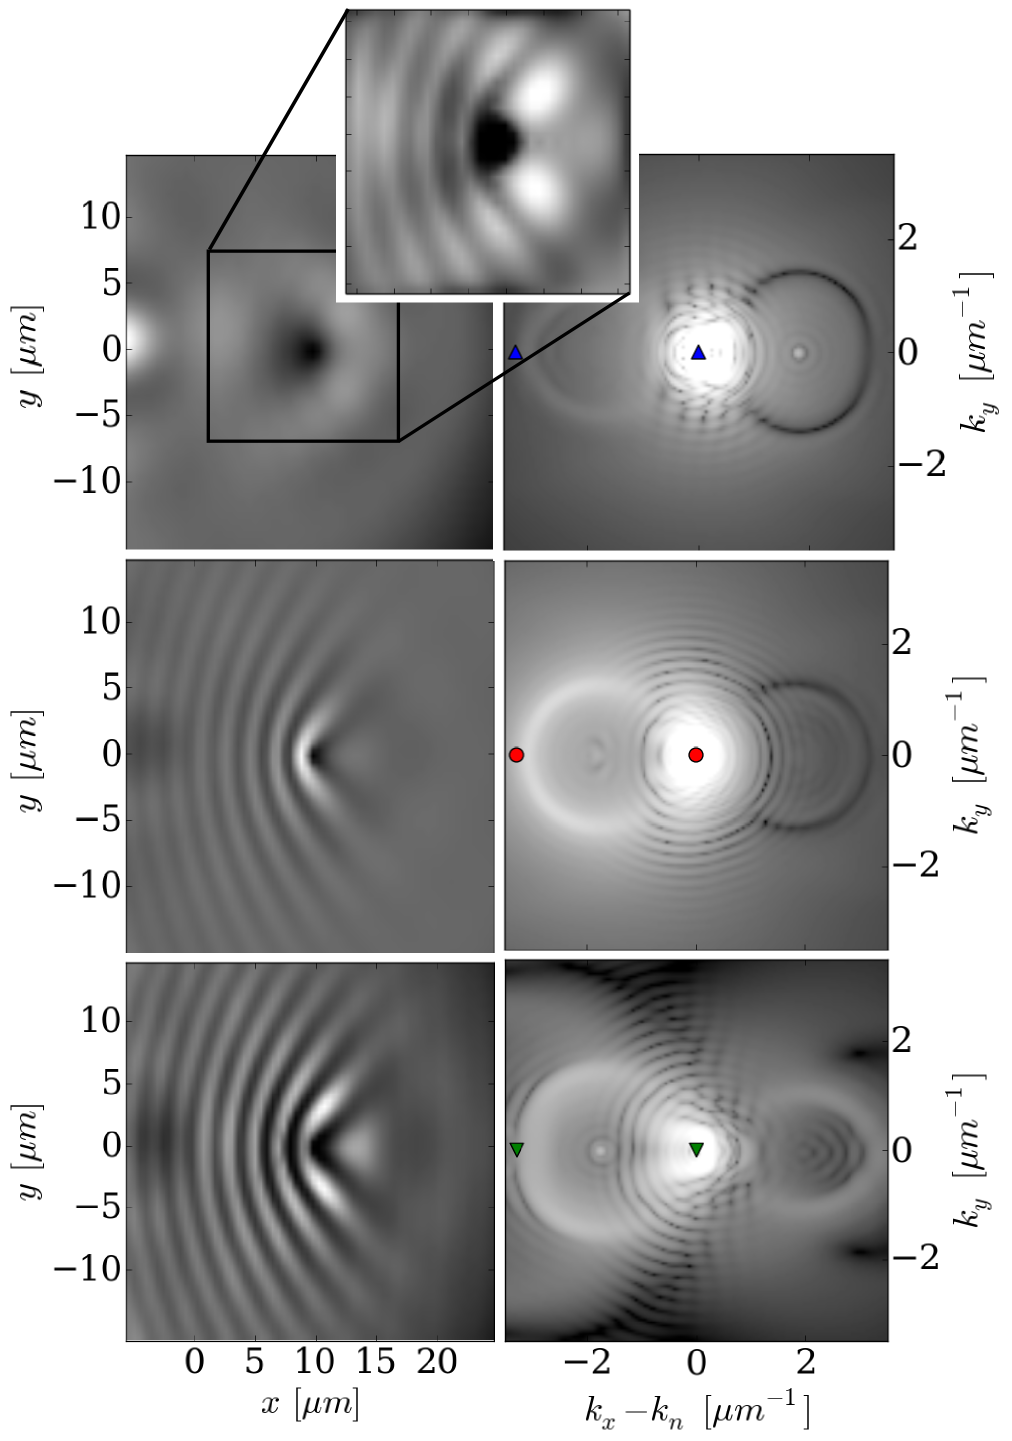
\includegraphics[width=.5\linewidth]{GP_space_mom}
% ~/Development/gp-linear-response/filtering-theory-GP.py
% ~/notebooks/julia/april/GP_signal_inset.ipynb
\caption{Full numerical responses to a static defect of
  the three OPO states in real and momentum space. Filtered OPO
  emissions (signal [top panels], pump [middle], and idler [bottom])
  in real space $|\psi_C (\vt{r},\omega_n)|^2$ (left panels in
  linear scale) and momentum space $|\psi_C
  (\tilde{\vt{k}},\omega_n)|^2$ (right panel in logarithmic scale)
  obtained by a full numerical evaluation of~\eqref{eq:gpequ}. For the
  top left panel of the signal space emission, Gaussian filtering is
  applied to enhance the short wavelength modulations of this state,
  revealing that the modulations corresponding to the pump state are
  also imprinted (though weakly) into the signal. The symbols indicate
  the pump ring diameter extracted from fitting the upstream
  modulations and resulting in a density wave wave-vector coinciding
  with the one of the pump $k_p=1.6$~$\mu$m$^{-1}$.}
\label{fig:numer}
\end{figure}
%
%%%%%%%%%%%%%%%%%%%%%%%%%%%%%%%%%%%%%%%%%%%%%%%%%
\section{Conclusions}
%
To conclude, we have reported a joint theoretical and experimental
study of the superfluid properties of a non-equilibrium condensate of
polaritons in the so-called optical parametric oscillator
configuration by studying the scattering against a static defect.
%
We have found that while the signal is basically free from
modulations, pump and idler lock to the same response. We have
highlighted the role of the coupling between the OPO components by
non-linear and parametric processes. These are responsible for the
transfer of the spatial modulations from one component to the
other. This process is most visible in the clear spatial modulation
pattern that is induced by the non-superfluid pump onto the idler,
while the same modulations are only extremely weakly transferred into
the signal, because of its low characteristic wavevector, so much that
experimentally cannot be resolved.
%
The main features of the real- and momentum-space emission patterns
are understood in terms of Rayleigh scattering rings for each
component and a characteristic propagation length from the defect; the
rings are then transferred to the other components by nonlinear and
parametric processes.
%%
Our theoretical and experimental results stress the complexities and
richness involved when looking for superfluid behaviours in
non-equilibrium multicomponent condensates such as the ones obtained
in the optical parametric oscillation regime.


\section{Supplemental Material}


In the manuscript, we carry on a theoretical and experimental analysis
of the response of microcavity polaritons in the optical parametric
oscillator (OPO) regime to a static defect.
%
For the theoretical calculations we follow two independent approaches:
In the first approach, we exactly numerically solve the dynamics of
the two coupled Gross-Pitaevskii equations (GPEs) for the exciton and
cavity fields for the realistic case of a finite-size top-hat pump
profile $\mathcal{F}_p(\vt{r})$. In the second approach, we apply a
perturbative linear response approximation for the lower polariton
(LP) state which leads to semi-analytical results in the limiting case
of a spatially homogeneous pump profile. Both methods have been
already successfully used in the literature to explore several
properties of the OPO operation.

While all fundamental formulae and information has been given in the
main text, in this Supplementary Material (SM) we present some
additional details on both approaches that might be of interest to the
specialized reader.  In addition to that, we make use of the linear
response approach to examine some regimes that are hardly accessed
experimentally or within a full numerical approach, which however
allow to put the conclusions of our work into a broader perspective.


%%%%%%%%%%%%%%%%%%%%%%%%%%%%%%%%%%%%%%%%%%%%%%%%%
\section{Full numerics}
\label{sec:detun}
%
The classical driven-dissipative non-linear Gross-Pitaevskii equation
(GPE) for the coupled exciton and cavity fields $\psi_{X,C}
(\vt{r},t)$ ($\hbar=1$)
%
\begin{equation}
  i\partial_t \begin{pmatrix} \psi_X \\ \psi_C \end{pmatrix} =
  \hat{H} \begin{pmatrix} \psi_X \\ \psi_C \end{pmatrix}
  + \begin{pmatrix} 0 \\ F_p(\vt{r},t) \end{pmatrix}\; ,
\label{eq:numer}
\end{equation}
%
where
%
\begin{equation}
  \hat{H} = \begin{pmatrix} \omega^{X}_{-i\nabla} - i
    \frac{\gamma_X}{2} + g_X |\psi_X|^2 & \Omega_R/2 \\ \Omega_R/2 &
    \omega^C_{-i\nabla} - i \frac{\gamma_C}{2} + V_d \end{pmatrix} \;
  ,
\end{equation}
%
is solved numerically on a 2D grid of $N\times N=2^8\times 2^8$ points
and a separation of $0.47$~$\mu$m (i.e., in a box $L\times L =
121$~$\mu$m$\times 121$~$\mu$m) by using a 5$^{\text{th}}$-order
adaptive-step Runge-Kutta algorithm. Convergence has been checked both
with respect the resolution in space $L/N$ as well as in momentum
$\pi/L$, without~\cite{Marchetti_2010,9783642241857} as well as in
presence of the defect.
%
The same approach has been already used in previous publications from
some of the authors (for a review, see
Refs.~\cite{Marchetti_2010,9783642241857}).
%
As for the system parameters, we have considered a LP dispersion at
zero photon-exciton detuning, $\omega^C_0 = \omega^X_0$, a
dispersionless excitonic spectrum, $\omega^X_{\vt{k}} = \omega^X_0$
and a quadratic dispersion for photons $\omega^C_{\vt{k}} =
\omega^C_0 + k^2/2m_C$, with the photon mass $m_C=2.3 \times 10^{-5}
m_e$, where $m_e$ is the bare electron mass. The LP dispersion, $2
\omega_{\vt{k}}^{LP} = \omega_{\vt{k}}^{C} + \omega_{\vt{k}}^{X}
- \sqrt{(\omega_{\vt{k}}^{C} - \omega_{\vt{k}}^{X})^2 +
  \Omega_R^2}$ is characterised by a Rabi splitting $\Omega_R =
4.4$~meV. Further, the exciton and cavity decay rates are fixed to
$\gamma_X=\gamma_C=0.53$~meV.
%
For the defect we choose a $\delta$-like defect potential
%
\begin{equation}
  V_d(\vt{r}) = g_d \delta(\vt{r} - \vt{r}_0)\; ,
\end{equation}
%
where its location $\vt{r}_0$ is fixed at one of the $N \times N$
points of the grid.
%
Note that in a finite-size OPO, local currents lead to inhomogeneous
OPO profiles in within the pump spot, despite the external pump having
a top-hat profile with a completely flat inner
region~\cite{Marchetti_2010,9783642241857} --- as shown later, this
can be observed in the filtered OPO profiles evaluated in absence of a
defect shown as dashed lines in S.~Fig.~\ref{fig:rafull}.
%
We have thus chosen the defect location so that it lies in the
smoothest and most homogeneous part of the OPO profiles.

Also we have checked that our results do not qualitatively depend on
the strength $g_d$ (nor on the sign) of the defect potential, as far
as this does not exceed a critical value above which it destabilises
the OPO steady-state regime.
%
The pump, $F_p(\vt{r},t) = \mathcal{F}_p(\vt{r}) e^{i (\vt{k}_p
  \cdot \vt{r} - \omega_p t)}$, has a smoothen and rotationally
symmetric top-hat profile, $\mathcal{F}_p(\vt{r}) = \mathcal{F}_p(r)
= \frac{f_p}{2}[\tanh(\frac{r+\sigma_p}{r_0}) -
  \tanh(\frac{r-\sigma_p}{r_0})]$ with strength $f_p = 1.23
f_p^\text{th} = 0.053$~meV/$\mu$m and parameters $r_0 = 8.68~\mu$m,
$\sigma_p = 34.72~\mu$m.
%
We pump at $k_p=1.6$~$\mu$m$^{-1}$ in the $x$-direction, $\vt{k}_p =
(k_p,0)$, and at $\omega_p-\omega_X^0=-0.44$~meV, i.e., roughly
$0.5$~meV above the bare LP dispersion. By increasing the pump
strength $f_p$, we find the threshold $f_p^{\text{th}}$ above which
OPO switches on, leading to two conjugate signal and idler states.
%
We then fix the pump strength just above this threshold ($f_p=1.23
f_p^{\text{th}}$), where we find a steady state OPO solution which is
stable (see Ref.~\cite{9783642241857} for further details). In
absence of the defect, this condition corresponds to a signal state at
$k_s=-0.2$~$\mu$m$^{-1}$ and $\omega_s-\omega_0^X = -1.64$~meV and an
idler at $k_i=3.4$~$\mu$m$^{-1}$ and $\omega_i-\omega_0^X =
0.76$~meV. 
%
It is interesting to note that already very close to the
lower pump power threshold for OPO, the selected signal momentum is
very close to zero. This contrasts with what one obtains in the linear
approximation scheme, where instead just above the lower OPO threshold
there exists a broad interval of permitted values for $k_s$ (and thus
$k_i$) --- we will discuss further this ``selection problem'' for
parametric scattering later in the section ``Linear response''.


%
\begin{figure}[tb]\centering
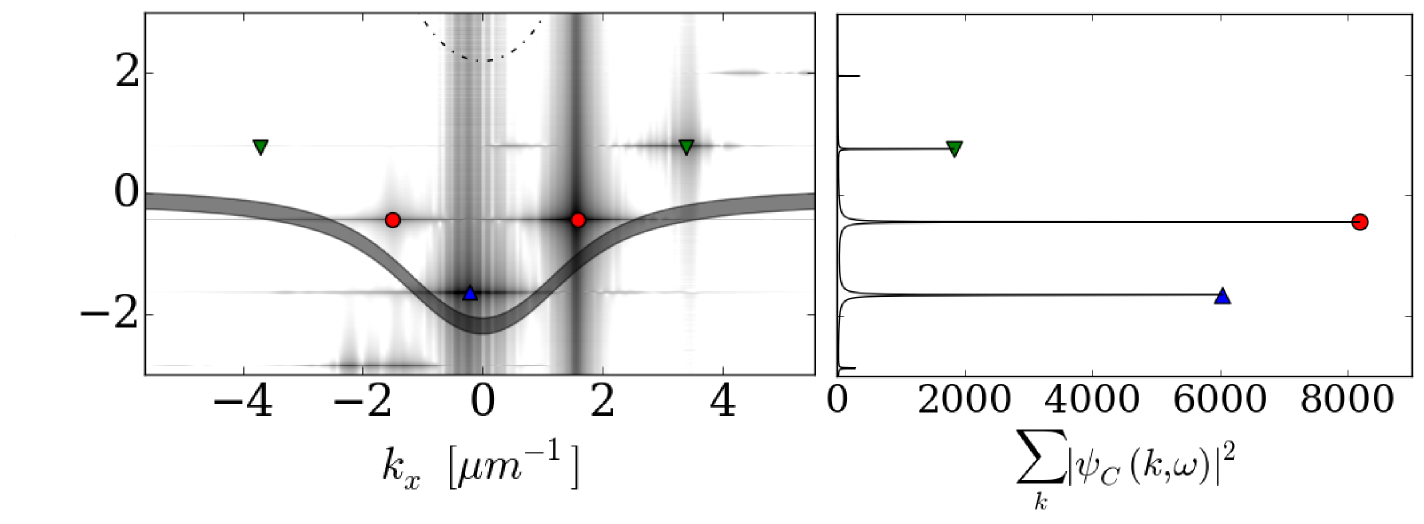
\includegraphics[width=.5\linewidth]{GP_disp}
% ~/notebooks/julia/theory-GP.ipynb
\caption{OPO spectrum obtained by full numerics. Left
  panel: Photonic component of the OPO spectrum in presence of a
  point-like defect, $|\psi_C(k_x,0,\omega)|^2$ (logarithmic scale),
  as a function of the rescaled energy $\omega - \omega_0^X$ versus
  the $x$-component of momentum $k_x$ (cut at $k_y=0$) for a top-hat
  pump (see text for the space profile and parameter values), with
  intensity $f_p=1.23 f_p^{\text{th}}$ above the OPO threshold, pump
  wave-vector $k_p=1.6$~$\mu$m$^{-1}$ in the $x$-direction and
  $\omega_p-\omega_X^0=-0.44$~meV. The symbols indicate the signal
  ([blue] upper triangle), pump ([red] circle), and idler ([green]
  lower triangle) energies, as well as the two momenta $k_x$ on each
  state Rayleigh ring at $k_y=0$. Note that the logarithmic scale
  results in a fictitious broadening in energy of the spectrum, which
  is in reality $\delta$-like (see right panel). The bare LP
  dispersion, including its broadening due to finite lifetime, is
  plotted as a shaded grey region, while the bare UP dispersion as a
  (black) dot-dashed line. Right panel: Momentum integrated spectrum,
  $\sum_{\vt{k}} |\psi_C(\vt{k},\omega)|^2$ (linear scale) as a
  function of the rescaled energy $\omega - \omega_0^X$, where it can
  be clearly appreciated that the emission is $\delta$-like in
  energy.}
\label{fig:spectGP}
\end{figure}
%
\begin{figure}[tb]\centering
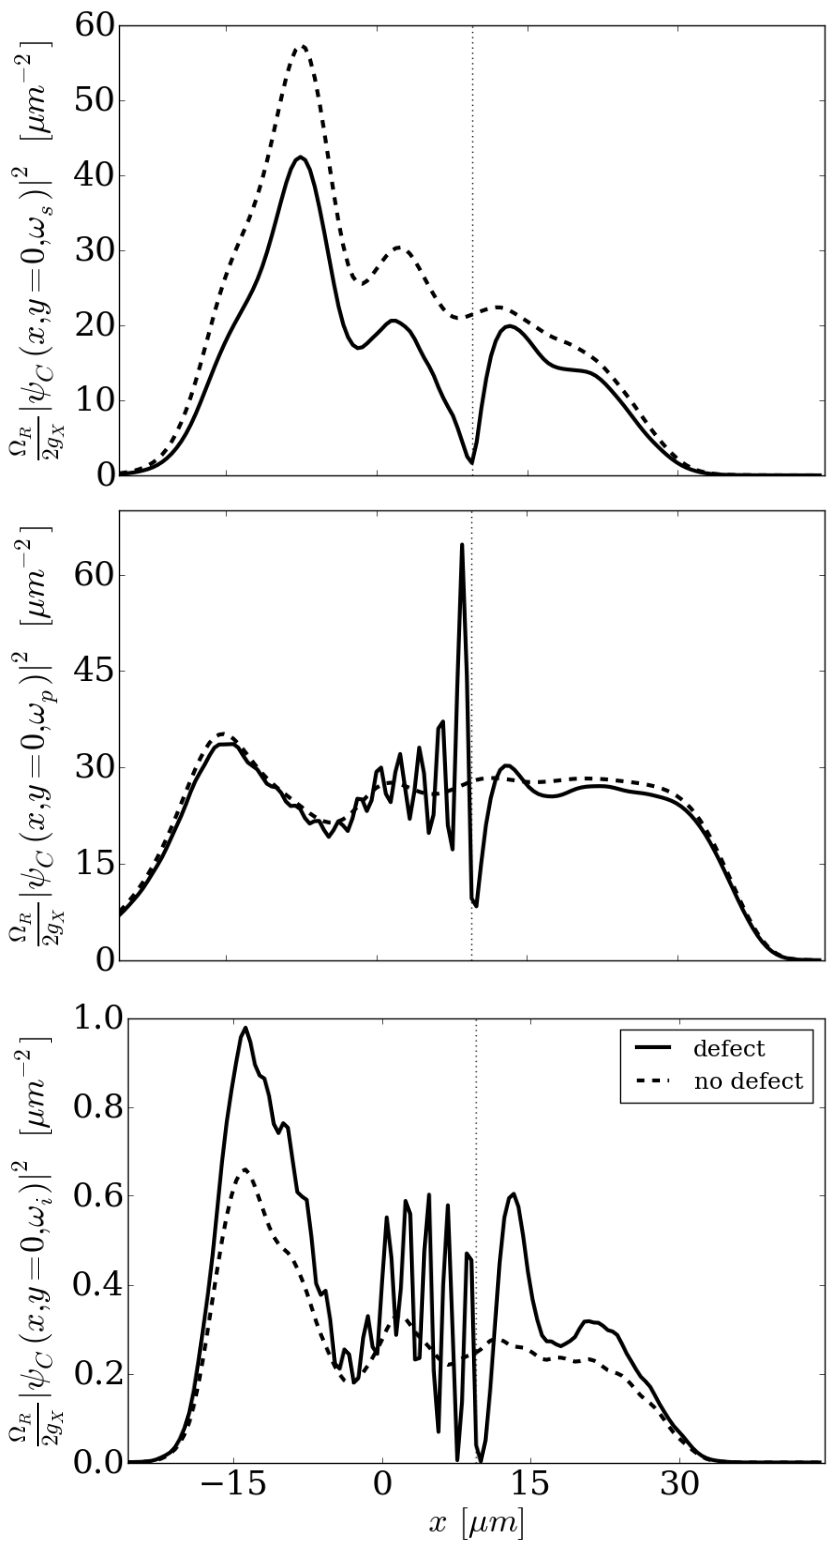
\includegraphics[width=.5\linewidth]{rangesGP.png}
% ~/Development/gp-linear-response/filtering-theory-GP.py
\caption{Real space signal, pump and idler OPO one-dimensional
  filtered profiles derived from finite size numerics with and without
  a defect. Rescaled OPO filtered emissions along the $y=0$ direction,
  $|\psi_C(x,y=0,\omega_n)|^2 \frac{\Omega_R}{2g_X}$, obtained by
  numerically solving the GPE Eq.~(1) of the main manuscript. While
  the dashed lines represent the filtered emissions of signal (top
  panel), pump (middle) and idler (bottom) for a top-hat pump without
  a defect, the solid lines are the same OPO conditions but now for a
  defect positioned at $(x_d, y_d) = (9.5, -0.5)$~$\mu$m corresponding
  to the vertical dotted lines. The system parameters are the same
  ones as those of Fig.~4 of the main manuscript.}
\label{fig:rafull}
\end{figure}
%
We evaluate the time dependent full numerical solution
of~\eqref{eq:numer} $\psi_{X,C} (\vt{r},t)$, until a steady state
regime is reached. Here, both its Fourier transform to momentum
$\vt{k}$ and energies $\omega$ can be evaluated numerically.
%
We plot on the left panel of S.~Fig.~\ref{fig:spectGP} a cut at $k_y=0$
of the photonic component of the OPO spectrum in presence of a
point-like defect, $|\psi_C(k_x,0,\omega)|^2$, as a function of the
rescaled energy $\omega - \omega_0^X$ versus the $x$-component of
momentum $k_x$ (cut at $k_y=0$). In the right panel we plot instead
the corresponding momentum integrated spectrum, $\sum_{\vt{k}}
|\psi_C(\vt{k},\omega)|^2$.
%
Here, we can clearly see that the presence of the defect does not
modify the fact that the OPO emission for the OPO signal ([blue] upper
triangle), pump ([red] circle), and idler ([green] lower triangle)
states has a completely flat dispersion in energy, thus indicating
that a stable steady state OPO solution has been reached. Note that in
the spectrum map of the left panel of Fig.~\ref{fig:spect}, the
logarithmic scale results in a fictitious broadening in
energy. However, from the integrated spectrum plotted in linear scale
in the right panel of Fig.~\ref{fig:spect} one can clearly appreciate
that this emission is $\delta$-like, exactly as it happens for the
homogeneous OPO case~\cite{9783642241857}.
%
Thus the effect of the defect is to induce only elastic (i.e., at the
same energy) scattering; now the three OPO states emit each on its own
Rayleigh ring (given each by the symbols on the left panel of
S.~Fig.~\ref{fig:spectGP} which represent the rings at a cut for
$k_y=0$). This makes it rather difficult to extract the separated
signal, pump and idler profiles by filtering in momentum, as done
previously for the homogeneous case, but it still allows to filter
those profiles very efficiently in energy. In fact, because the
emission is $\delta$-like, it is enough to fix a single value of the
energy $\omega$ to the one of the three states $\omega_{n=s,p,i}$,
thus extracting the filtered profiles either in real space
$|\psi_C(\vt{r},\omega_n)|^2$ or in momentum space
$|\psi_C(\vt{k},\omega_n)|^2$ --- we have however checked that
integrating in a narrow energy window around $\omega_n$ does not
quantitatively change the results.

The results of the above described filtering are shown in Fig.~4 of
the manuscript.
%
In S.~Fig.~\ref{fig:rafull} we instead plot the corresponding
one-dimensional profiles in the $y=0$ direction both in presence
(solid line) and without (dashed line) a defect. Here, we can observe
that, even if the pump has a top-hat flat profile, as also commented
previously, in absence of a defect, the finite-size OPO is
characterised by inhomogeneous profiles of signal, pump and idler
because of localised currents. Further, we observe that the presence
of a defect induces strong modulations in pump and idler.
%
In order to reveal that the pump also imprints its modulation into the
signal, even though these are extremely weak (and hardly visible in
both the top main panel of Fig.~4 of the manuscript and the top panel
of S.~Fig.~\ref{fig:rafull}), we apply a Gaussian filtering to the
signal images, which result is shown in the inset of the top-left
panel of Fig.~4 in the manuscript.
%
This consists of the following procedure. The original data for the
real space profile $\psi(\vt{r})$ are convoluted with a Gaussian
kernel $K(\vt{r} - \vt{r}')$, obtaining a new profile,
$\tilde{\psi}(\vt{r}') = \int d\vt{r} \psi (\vt{r}) K(\vt{r} -
\vt{r}')$, where short wavelengths features are smoothen out. The
convoluted image $\tilde{\psi}(\vt{r}')$ is then subtracted from the
original data, giving $\psi(\vt{r}) - \tilde{\psi}(\vt{r})$, and
effectively filtering out all long wavelength details.
%
The same procedure of Gaussian filtering is also applied to the signal
emission profile obtained within the linear response analysis and
shown in the inset of the top left panel of Fig.~2 of the manuscript.

%
\begin{figure}[tb]\centering
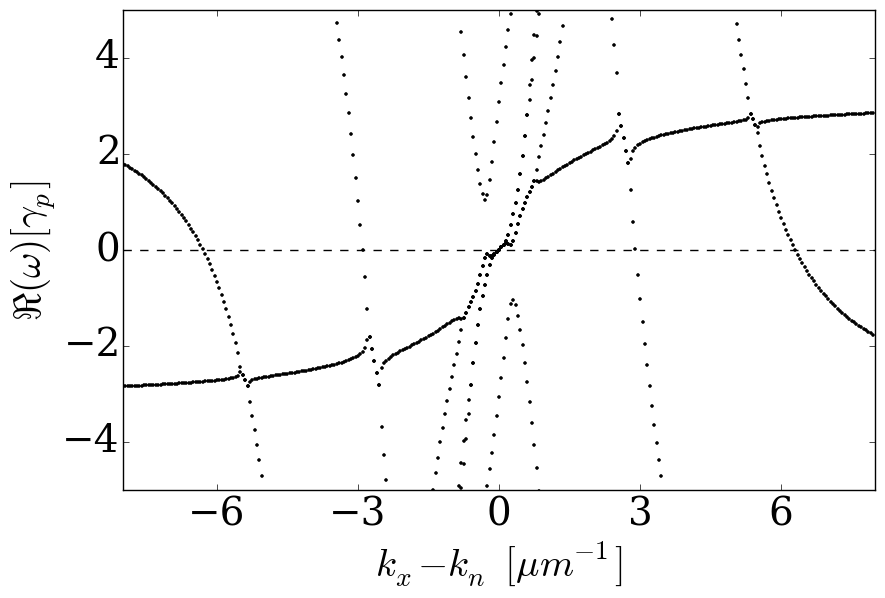
\includegraphics[width=.5\linewidth]{fig_excitation_ks_0_000.png}
% ~/notebooks/OPODrag/opodrag.py
\caption{Spectrum of collective excitations. Cut at $k_y=0$ of the
  real part of the quasiparticle energy dispersion $\Re
  \omega_{n,(u,v),\vt{k}-\vt{k}_n}$ plotted versus $k_x -
  k_n$. The spectrum is evaluated within the linear approximation
  scheme and the parameters are the same ones used for Fig.~2 of the
  main manuscript.}
\label{fig:bogol}
\end{figure}
%
%
\begin{figure}[tb]
\centering
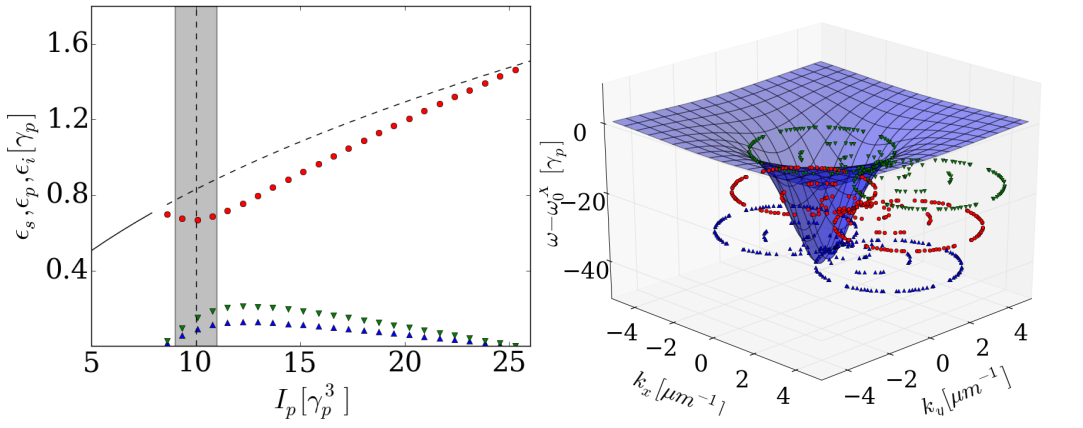
\includegraphics[width=.5\linewidth]{3d0_7.png}
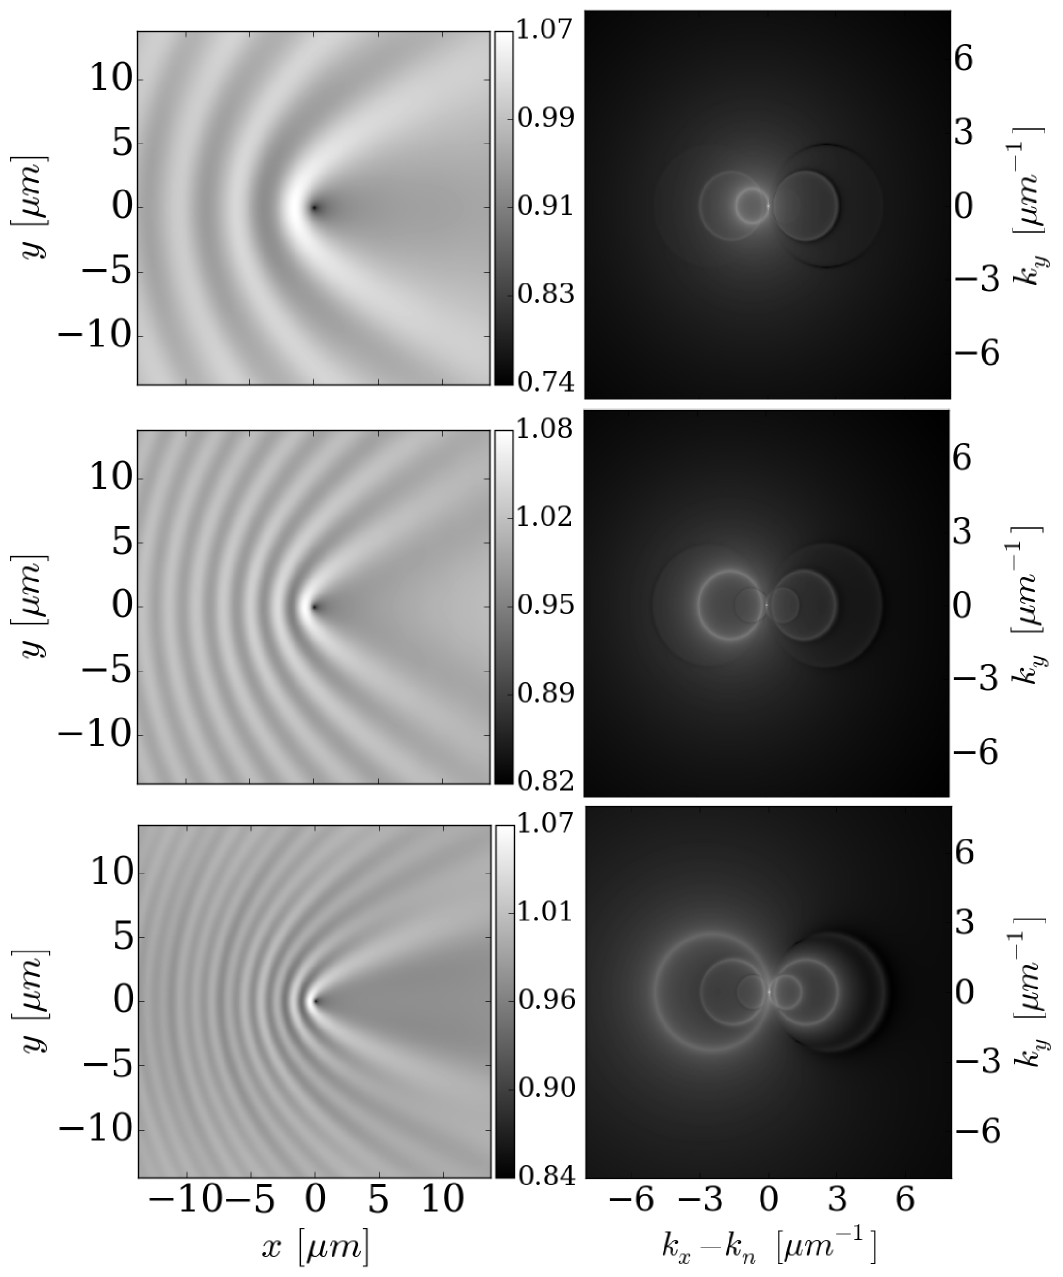
\includegraphics[width=.5\linewidth]{ks0_7.png}
% ~/notebooks/OPODrag/opodrag.py
\caption{OPO for finite and positive signal momentum in
  the linear response approximation for homogeneous pumping. Rescaled
  OPO emission within the linear response approximation in real $|\psi
  (\vt{r},\omega_n)|^2/|\psi_n|^2$ (left panels in linear scale) and
  momentum space $|\psi_{\tilde{\vt{k}}} (\omega_n)|^2$ (right
  panels in linear scale) filtered at the energies of the three OPO
  states: signal (top panels), pump (middle), and idler (bottom). The
  parameters are the same as those used in Fig.~2 of the main
  manuscript, with the exception of the signal and idler momenta,
  which are now at $k_s = 0.7$~$\mu$m$^{-1}$ and $k_i =
  2.5$~$\mu$m$^{-1}$ respectively. Each scale of variation for the
  profiles is plotted in the color-box next to the left panels. A cut
  in the $y=0$ direction for the three profiles is plotted in the
  bottom panel of S.~Fig.~\ref{fig:range}.}
\label{fig:ksp07}
\end{figure}
%
%
\begin{figure}[tb]
\centering
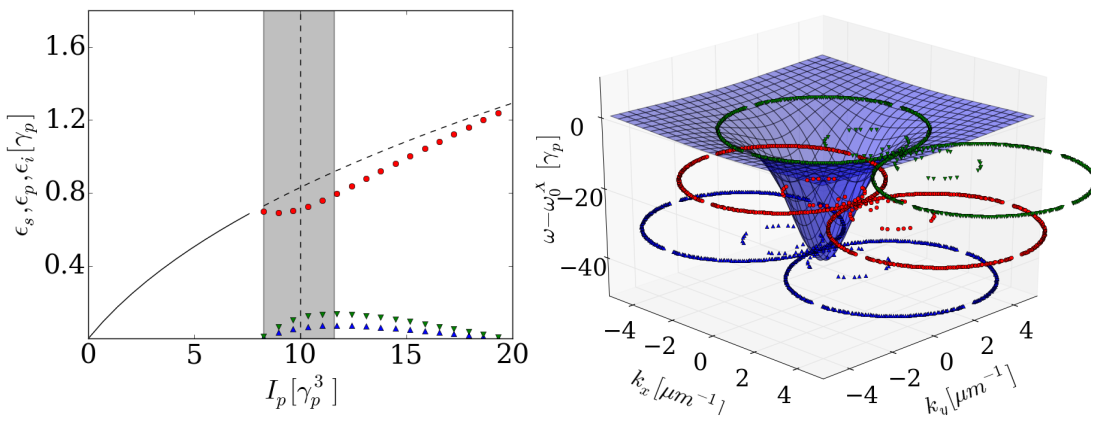
\includegraphics[width=.5\linewidth]{3d-0_4.png}
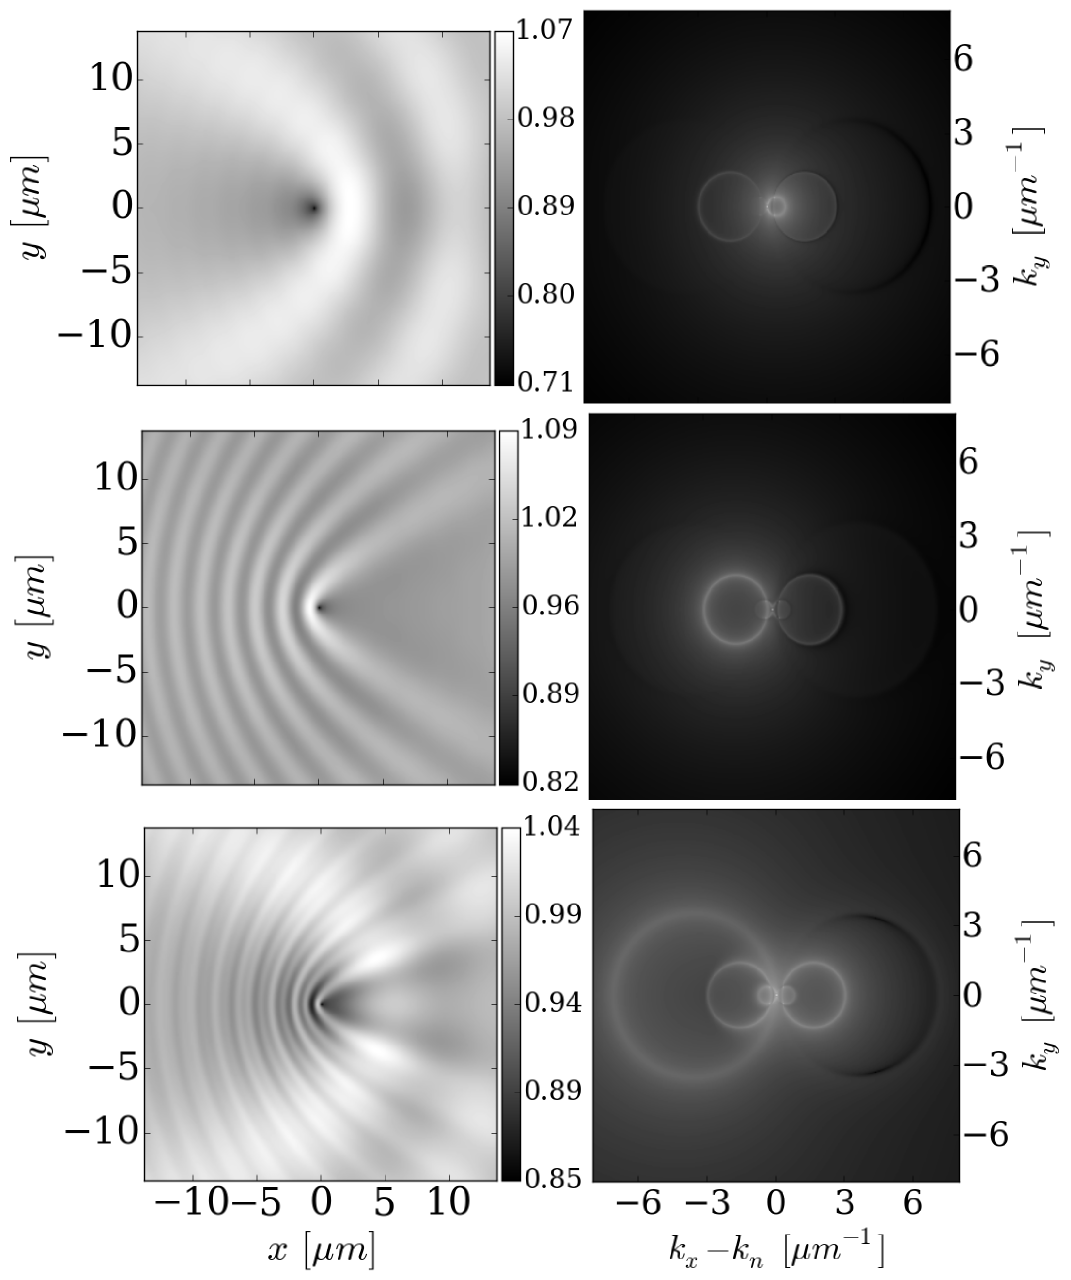
\includegraphics[width=.5\linewidth]{ks-0_4.png}
% ~/notebooks/OPODrag/opodrag.py
\caption{OPO for finite and negative signal momentum in
  the linear response approximation for homogeneous pumping. Rescaled
  OPO emission within the linear response approximation in real $|\psi
  (\vt{r},\omega_n)|^2/|\psi_n|^2$ (left panels in linear scale) and
  momentum space $|\psi_{\tilde{\vt{k}}} (\omega_n)|^2$ (right
  panels in linear scale) filtered at the energies of the three OPO
  states: signal (top panels), pump (middle), and idler (bottom). The
  parameters are the same as those used in Fig.~2 of the main
  manuscript, with the exception of the signal and idler momenta,
  which are now at $k_s = -0.4$~$\mu$m$^{-1}$ and $k_i =
  3.6$~$\mu$m$^{-1}$ respectively. A cut in the $y=0$ direction for
  the three profiles is plotted in the top panel of
  S.~Fig.~\ref{fig:range}.}
\label{fig:ksm04}
\end{figure}
%
\begin{figure}[tb]\centering
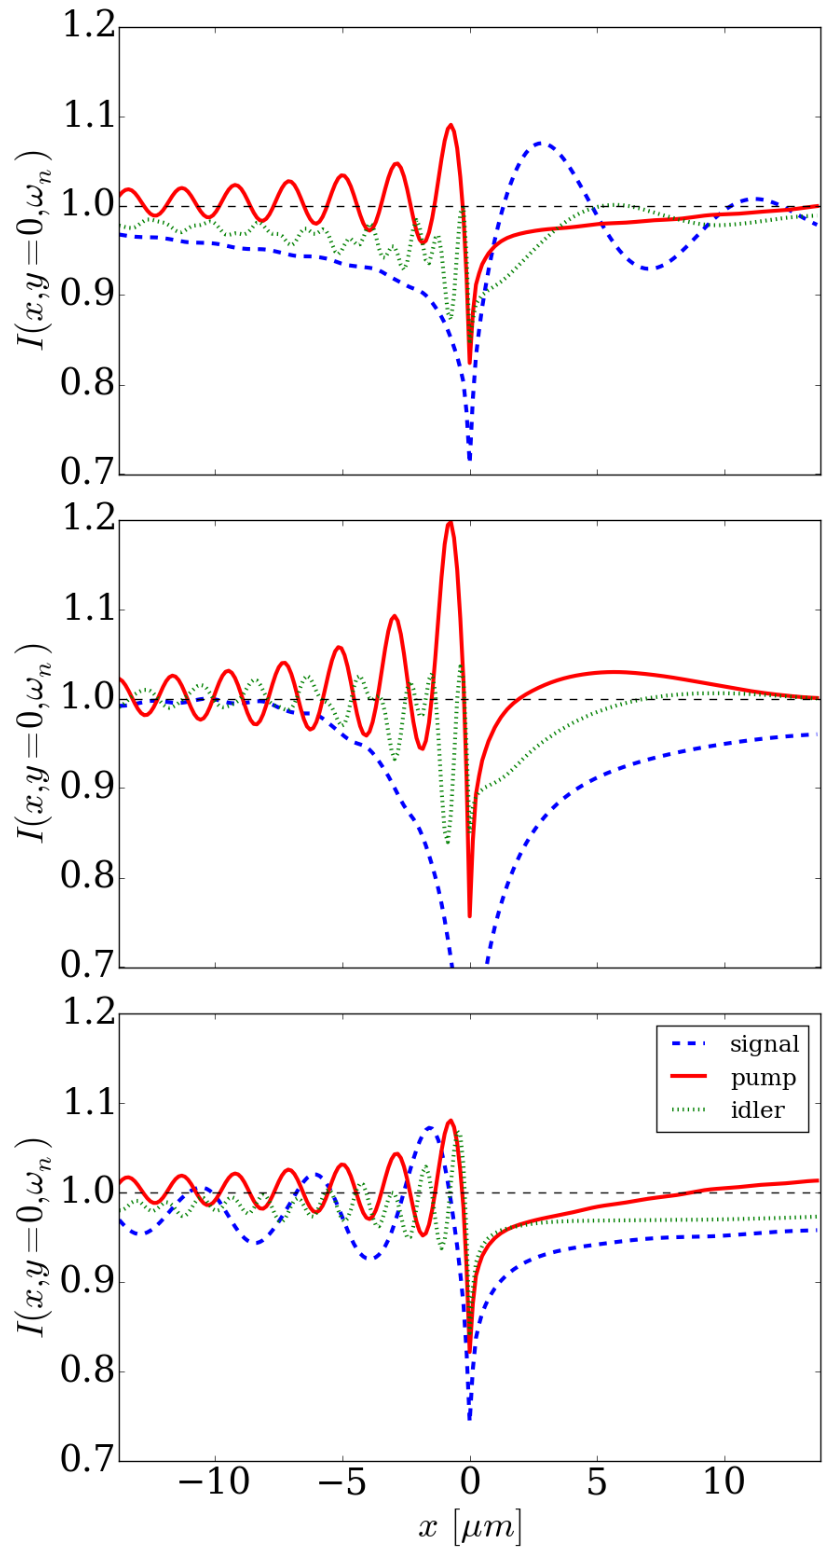
\includegraphics[width=.5\linewidth]{ranges.png}
% ~/notebooks/OPODrag/opodrag.py
\caption{Real space signal, pump and idler OPO
  one-dimensional filtered profiles in the linear response
  approximation. OPO filtered emissions along the $y=0$ direction, $I
  (x, y=0, \omega_n) = |\psi(x,y=0, \omega_n)|^2/|\psi_n|^2$ rescaled
  by the mean-field solution $\psi_n$ in absence of the defect, for
  the three cases analysed above within the linear response
  approximation: the case of a signal at $k_s = -0.4$~$\mu$m$^{-1}$
  (top panel) corresponds to the same conditions as
  S.~Fig.~\ref{fig:ksm04} , a signal at $k_s = 0.0$~$\mu$m$^{-1}$
  (middle panel) corresponds to Fig.~2 of the main manuscript, and a
  signal at $k_s = 0.7$~$\mu$m$^{-1}$ (bottom panel) corresponds to
  S.~Fig.~\ref{fig:ksp07}. In each panel we plot, on the same linear
  scale, the filtered profiles of signal ([blue] dashed line), pump
  ([red] solid), and idler ([green] dotted), while the horizontal gray
  dashed lines represent the values of the mean-field emission prior
  to adding a defect (rescaled here to $1$).}
\label{fig:range}
\end{figure}
%
\begin{figure}[tb]\centering
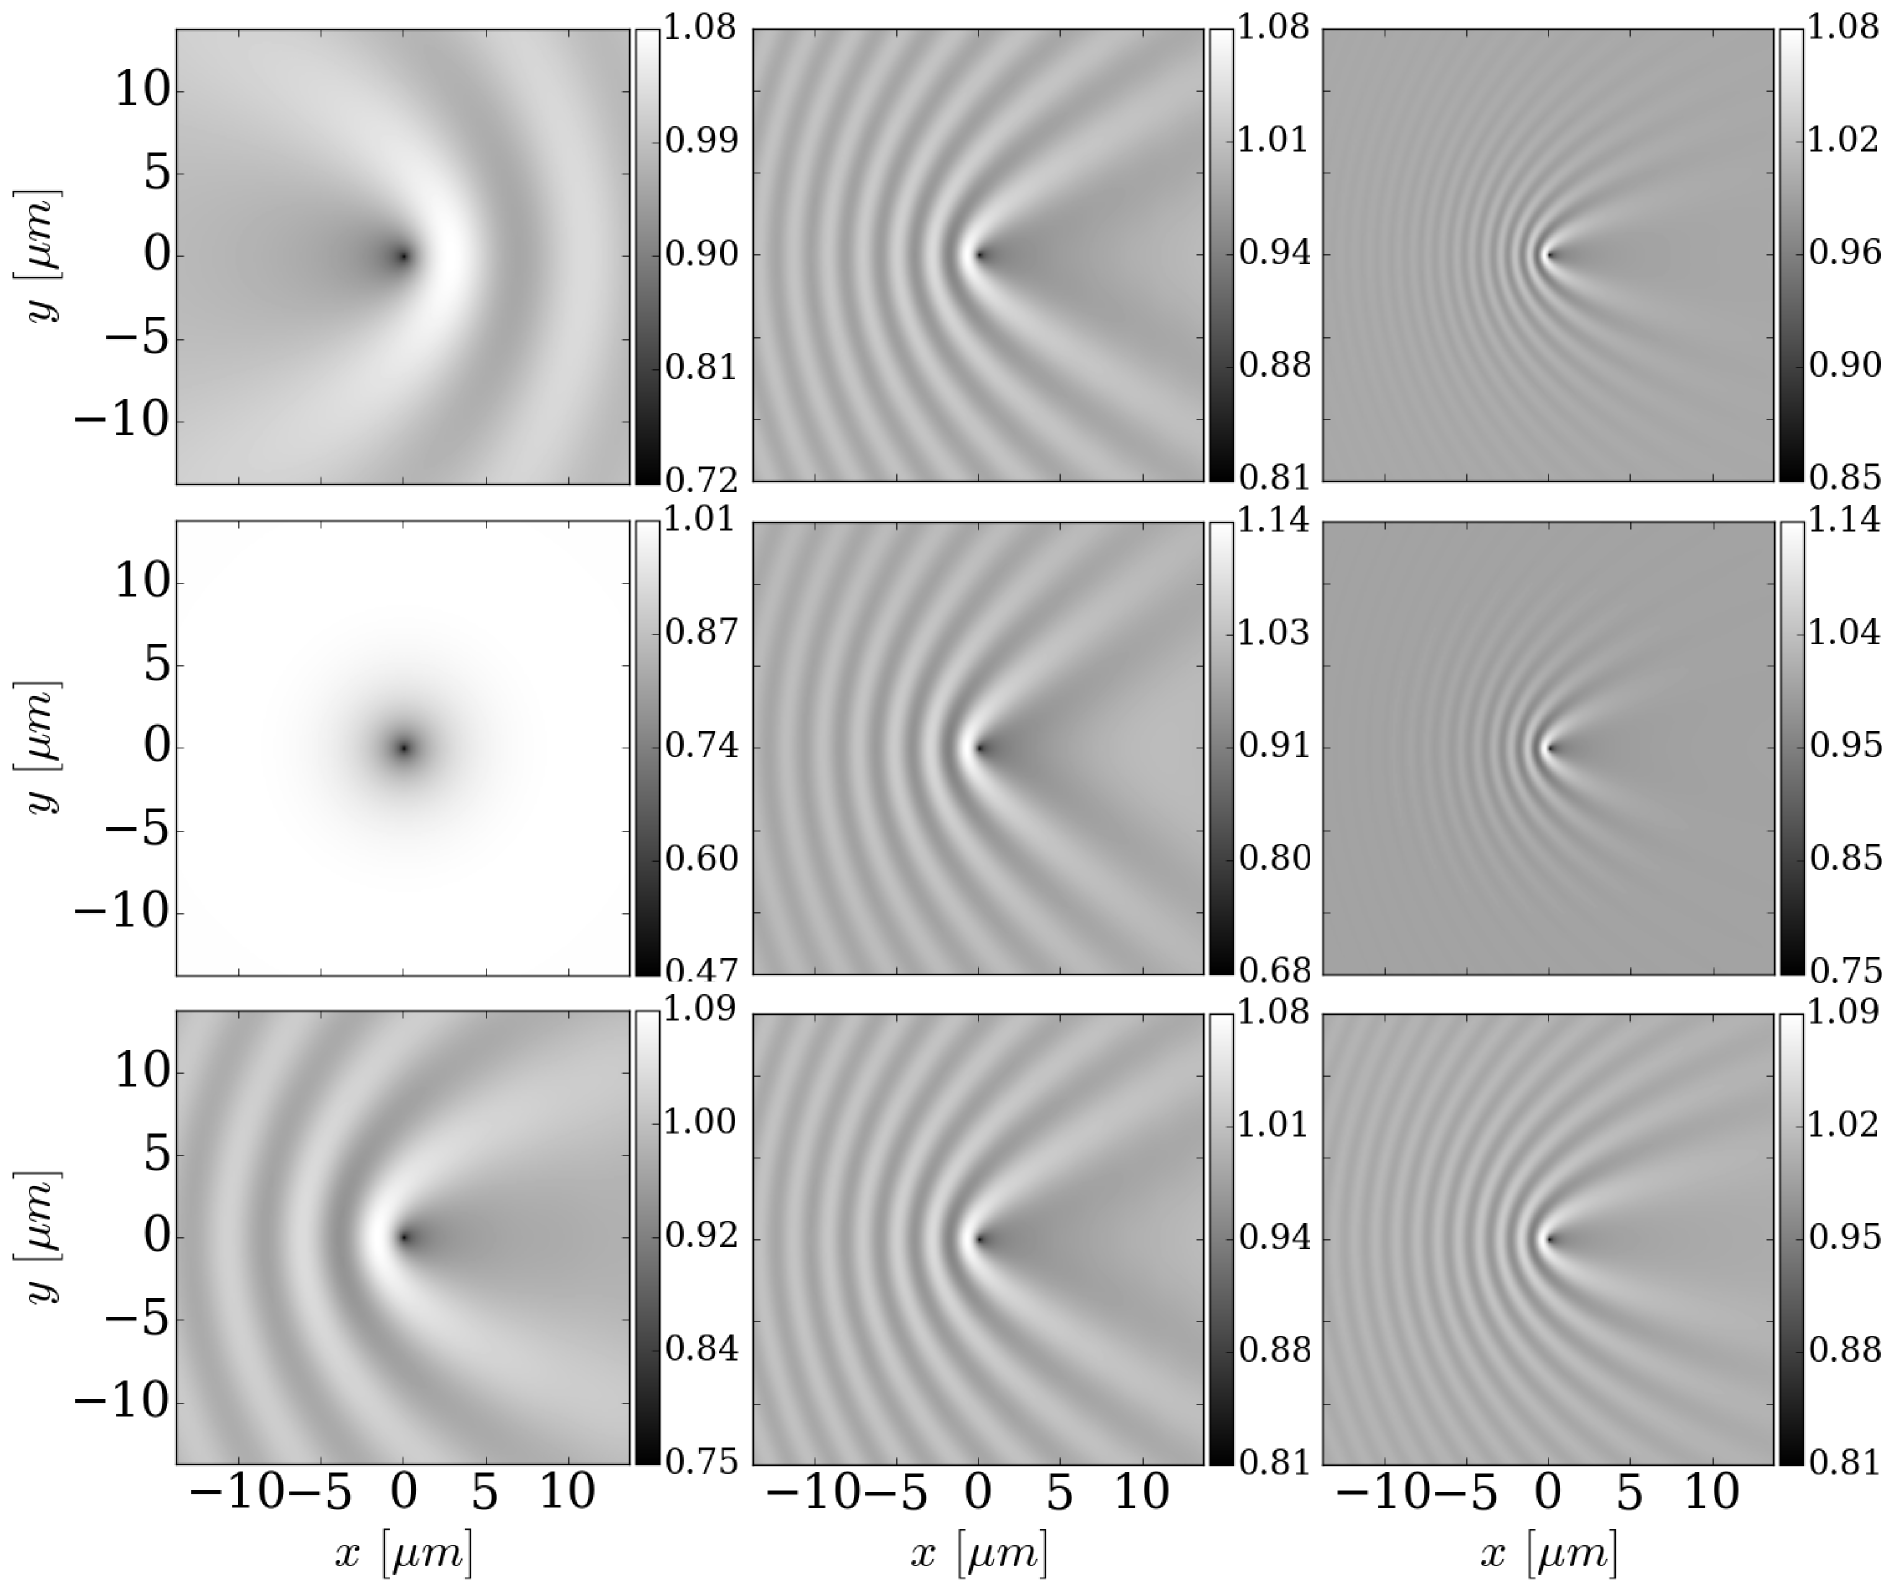
\includegraphics[width=.5\linewidth]{uncoupled.png}
% ~/notebooks/OPODrag/opodrag.py
\caption{Real space profiles of three uncoupled signal, pump and idler
  fluids. The rescaled profiles $|\psi
  (\vt{r},\omega_n)|^2/|\psi_n|^2$ are obtained by setting all
  off-diagonal couplings in Eq.~(6) of the main manuscript to zero,
  resulting in three uncoupled signal (left column), pump (middle
  column), and idler (right column) fluids. The three rows correspond
  to the three different cases previously analysed within the linear
  response approximation: the case of a signal at $k_s =
  -0.4$~$\mu$m$^{-1}$ (top row) corresponds to the same conditions as
  S.~Fig.~\ref{fig:ksm04} , a signal at $k_s = 0.0$~$\mu$m$^{-1}$
  (middle row) corresponds to Fig.~2 of the main manuscript, and a
  signal at $k_s = 0.7$~$\mu$m$^{-1}$ (bottom row) corresponds to
  S.~Fig.~\ref{fig:ksp07}.}
\label{fig:uncou}
\end{figure}
%
%%%%%%%%%%%%%%%%%%%%%%%%%%%%%%%%%%%%%%%%%%%%%%%%%
\section{Linear response}
\label{sec:analy}
%
In the manuscript we also make use of the linear response
approximation to analyse the OPO response to a static defect, valid
for a homogeneous pump scheme. In order to do so, we first evaluate
the Bogoliubov matrix given in Eq.~(6) of the manuscript, whose
eigenvalues determine the spectrum of collective excitations. We plot
in S.~Fig.~\ref{fig:bogol} a typical collective dispersion (here we
consider the same system parameters as the ones used in Fig.~2 of the
manuscript), by plotting the real part of the Bogoliubov matrix
eigenvalues $\Re \omega_{n,(u,v),\vt{k}-\vt{k}_n}$ as a function
of $k_x - k_n$ (cut at $k_y=0$). Note that the Rayleigh rings can be
found by finding the intersections $\Re
\omega_{n,(u,v),\vt{k}-\vt{k}_n}=0$.


As also done for the full numerics, we
consider there a $\delta$-like disorder potential $V_d(\vt{r}) = g_d
\delta(\vt{r} - \vt{r}_0)$, and Figs.~1 and~2 of the manuscript,
as well as S.~Figs.~\ref{fig:ksp07} and~\ref{fig:ksm04} below, are
plotted for this case.
%
We have however checked that our results do not depend on the specific
shape of the defect potential: In particular we have also considered
the response to defects with smoothen Gaussian-like profiles, whose
effect is only to partially weaken the upstream modulations emission
in real space.

We have seen in the manuscript that both experimentally as well as in
the full numerical analysis, one obtains OPO conditions where the
signal momentum is very close to zero, $\vt{k}_s \sim 0$. The reason
why OPO selects almost zero momentum signal conditions is still
awaiting a theoretical explaination.
%
In contrast, the linear response approximation allows to access very
different OPO mean-field conditions, for which, by leaving unaltered
the value of the pump momentum, the signal can appear at finite
momentum values, either positive or negative.
%
This is a peculiarity of this approximation scheme, where one can show
that, at mean-field level, one has the possibility of choosing
different values of the signal momentum $\vt{k}_s$ (and thus the one
of the idler $\vt{k}_i$), and that this choice range is quite broad
particularly when the pump power is close to the lower pump threshold
for OPO --- the stability region for OPO is plotted as a shaded grey
region in the top left panels of S.~Figs.~\ref{fig:ksp07}
and~\ref{fig:ksm04}. This is a well known ``selection problem'' for
parametric scattering (see Ref.~\cite{Wouters_2007_b}): The reason why
in full numerical calculations, parametric scattering processes select
a signal with a momentum close to zero, already very close to the
lower pump thresold for OPO, is still awaiting for an explaination. In
particular, this quest cannot be addressed within a spatially
homogeneous approximation where the three mean-field solutions for
pump, signal, and idler states can be describes by plane waves.
%%
One can only show that, within the same mean-field approximation
scheme, when increasing the pump power towards the upper threshold for
OPO, the blue-shift of the LP polariton dispersion due to the
increasing mean-field polariton density, causes the signal momentum to
converge towards zero~\cite{Whittaker_2005} $\vt{k}_s \rightarrow 0$.

%%%%%%%%%%%%%%%%%%%%%%%%%%%%%%%%%%%%%%%%%%%%%%%%%
\paragraph{OPO conditions with a finite momentum signal ---}
%
Given the freedom of choice for the signal momentum $\vt{k}_s$ close
to the lower OPO threshold, we consider here two additional cases,
that could not be studied neither experimentally, nor within a full
numerical approach, but that instead we can easily analyse within the
linear response theory.
%
In particular, we have left fixed the pumping conditions
$k_p=1.6$~$\mu$m$^{-1}$ and $\omega_p-\omega_X^0=-1.25$~meV and
considered two opposite situations.


In the first case, the signal has a finite and positive momentum $k_s
= 0.7$~$\mu$m$^{-1}$ and thus the idler is at low momentum, $k_i
=2.5$~$\mu$m$^{-1}$. The results are shown in S.~Fig.~\ref{fig:ksp07}.
%
Here we see that all six Rayleigh rings are clearly visible and, in
addition, as the idler is at lower momentum compared to the case
considered in Figs.~1 and~2 of the manuscript, and thus its dispersion
steeper, the idler group velocity is large enough to appreciate the
modulation of the Rayleigh ring associated to this state. As a result,
each of the three filtered OPO emissions exhibits as the strongest
modulation the one coming from its own Rayleigh ring, included the
signal which is now at finite and large momentum. In this case, the
OPO response of each filtered state profile looks completely
independent from the other, as if we were pumping each state
independently.

In the second case shown in S.~Fig.~\ref{fig:ksm04} , the signal is
finite and negative, $k_s = -0.4$~$\mu$m$^{-1}$, and the idler is now
at very large momentum, $k_i = 3.6$~$\mu$m$^{-1}$, where its
dispersion is very exciton-like and flat, and thus the idler has a
very small group velocity and its own modulations are visible only
very close to the defect. For this case, we can appreciate in the
idler filtered profile overlapped modulations from all the three state
Rayleigh rings (note that because the signal is at negative momentum,
its modulations have an opposite direction compared to the ones of
pump and idler), while in the signal we can mostly see the signal long
wavelength modulations and only very weakly the pump one.


We can compare the different modulation strengths of the three OPO
profiles by looking at the color bars plotted next to the profiles. In
order to better compare them on the same plot, we show in
S.~Fig.~\ref{fig:range} the one-dimensional OPO filtered emissions
along the $y=0$ direction for the three cases analysed above. While
for the OPO conditions with a signal at $k_s = 0.0$~$\mu$m$^{-1}$
(middle panel, corresponding to Fig.~2 of the main manuscript), the
imprinted modulations from the pump are hardly visible, and can only
be appreciated after a Gaussian filter manipulation, both OPO cases
with a finite momentum signal result in modulations in the signal with
an amplitude of the same order of magnitude of both pump and idler
fluids.

In S.~Fig.~\ref{fig:uncou} we instead show the real space profiles
obtained by setting all off-diagonal couplings in the Bogoliubov
matrix $\mathcal{L}_{\vt{k}}$ of Eq.~(6) of the main manuscript to
zero, resulting in three uncoupled signal (left column), pump (middle
column), and idler (right column) fluids. This underlines the
importance of the coupling between the three fluids in the three
different OPO regimes previously analysed within the linear response
approximation. In particular, for the OPO conditions such that the
signal has a finite and positive momentum $\vt{k}_s$ (bottom row of
S.~Fig.~\ref{fig:uncou}, which corresponds to the conditions shown in
S.~Fig.~\ref{fig:ksp07}), the coupling has little effect and the three
fluid respond to the defect in practice in a independent way (each
Rayleigh ring influences its own fluid). The OPO condition with a
finite and negative momentum $\vt{k}_s$, which corresponds to the
conditions shown in S.~Fig.~\ref{fig:ksm04}, are shown in the top row
of S.~Fig.~\ref{fig:uncou}: Here, we can see that the coupling between
the three fluids plays an effect. The modulations of the pump can be
appreciated both in the signal profile (though weakly), as well as in
the idler profile. In the idler fluid its own modulations can only
propagate very close to the defect and thus the only really
appreciable modulations are the ones inherited from the pump. Finally,
for the experimentally relevant case of an OPO with a signal at zero
momentum (middle row of S.~Fig.~\ref{fig:uncou}, which corresponds to
the conditions shown in Fig.~2 of the manucript), there is also a role
played by the coupling, though, as already thoroghly analysed, the
modulations in the signal inhereted from the pump can only be
appreciated after a Gaussian filtering manipulation.


Finally note that, as it also happens for the OPO conditions shown in
Fig.~1 of the manuscript, the subsonic to supersonic crossover of the
pump-only state~\cite{Amo_2009} happens at pump intensities well above
the region of stability of OPO --- the shaded gray regions of
S.~Figs.~\ref{fig:ksp07} and~\ref{fig:ksm04} Thus, it is not possible
to study a case where the pump is already subsonic and at the same
time promotes stimulated scattering.



%%% Local Variables:
%%% mode: latex
%%% TeX-master: "../thesis_berceanu"
%%% End:

%%%%%%%%%%%%%%%%%%%%%%%%%%%%%%%%%%%%%%%%%%%%
% Key                         | Occurences |
%-----------------------------+------------|
% price2014magnetic           |         14 |
% ozawa2014momhh              |          9 |
% hafezi2013imaging           |          7 |
%%%%%%%%%%%%%%%%%%%%%%%%%%%%%%%%%%%%%%%%%%%%

% TODO: add updates from Hannah's proceedings
% TODO: add Hannah's new figure(s) from proceedings
% TODO: cite conference proceedings .~\cite{proceeding}

\chapter{Landau levels in driven-dissipative cavity arrays}
\label{cha:landau}

\section{Introduction}

A planar system of electrons in a strong magnetic field is the
archetypal model for studying phenomena such as the integer and
fractional quantum Hall effects. With recent advances in creating
synthetic gauge fields, however, new horizons have opened up for
simulating such topological phases of matter also with neutral
particles, such as photons~\cite{hafezi2014synthetic} or ultracold
atoms~\cite{dalibardrmp2011, goldman_repprog_2014,
Goldman_arxiv_2015}.  Rather than simply replicating previous
measurements, experiments with synthetic gauge fields allow for
unprecedented access to properties such as the eigenstates or
eigenspectrum, while the tunability and controllability of these
experiments offer the prospect of simulating novel physics.

In the presence of a (synthetic) gauge field, the eigenstates making
up an energy band can have nontrivial geometrical properties, as
encoded in the Berry connection and Berry curvature defined
below~\cite{berry, xiao2010berryreview}. Understanding the geometry of
eigenstates in a band is of great importance, not least because the
integral of the Berry curvature over the 2D Brillouin zone (BZ) gives
the first Chern number: the topological invariant responsible for the
integer quantum Hall effect~\cite{thouless}. Consequently, there has
been much work in recent years to develop new techniques with which to
probe the properties of energy bands in photonics and ultracold
gases. For example, the Berry curvature can be measured in the
semiclassical dynamics of a wavepacket in an optical
lattice~\cite{dudarev,1chang, price, cominotti, dauphin,
aidelsburger2015measuring, jotzu2014experimental} or in photon
transport in a cavity array~\cite{ozawa2014qhe}. In all these cases,
the physics can be most naturally understood by recognising that the
Berry curvature acts like a magnetic field in momentum
space~\cite{berry, bliokh2005spin, PhysRevD.12.3845,
cooper2012designing}.

The analogy between Berry curvature and magnetism is most powerful
when a geometrical energy band is subjected to an additional weak
harmonic potential~\cite{price2014magnetic}. Then, in the effective
momentum-space Hamiltonian, a harmonic potential acts like the kinetic
energy of a particle in real space. Just as the physical momentum
$\vt{p}-\vt{A}(\rv)$ is the sum of the canonical momentum $\vt{p}$ and
the magnetic vector potential $\vt{A} (\rv)$ in the magnetic
Hamiltonian, so the physical position $\vt{r}+\mathcal{A}_{n,n}(\pv)$,
is given by the canonical position $\vt{r}$ and the Berry connection
$\mathcal{A}_{n,n}(\pv)$ of band $n$ in the effective
Hamiltonian~\cite{adams1959energy,nagaosa,
murakami2003dissipationless, bliokh2005spin, fujita,
bliokh2005topological,gosselin2006semiclassical}. The Berry curvature,
$\Omega_n (\pv)= \nabla \times \mathcal{A}_{n,n}(\pv)$, is then like a
momentum-space magnetic field. For certain models, this analogy leads
to a clear analytical understanding of single-particle
dynamics~\cite{price2014magnetic, ozawa2014momhh, price2015sporbit,
Claassen_prl_2015}. In particular, we will focus on the small-flux
limit of the Harper-Hofstadter
Hamiltonian~\cite{harper1955magnetic,hofstadter1976butterfly}, which
is a model that has recently been realized in a multitude of
experimental configurations, ranging from ultracold
gases~\cite{aidelsburger2013hh,miyake2013hh,mancini2015edge,stuhl2015edge},
solid state superlattices~\cite{dean2013hofstadter,yu2014hierarchy}
and silicon photonics~\cite{hafezi2013imaging} to classical systems
such as coupled pendula~\cite{susstrunk2015pendula} and oscillating
circuits~\cite{jia2013circuits}. As first shown in
Ref.~\cite{price2014magnetic}, the eigenstates of this model in the
presence of a harmonic trap are toroidal Landau levels in momentum
space. Not only would an observation of these states constitute the
first exploration of analogue magnetic states in momentum space, but
also the first experimental study of magnetism on a torus.
 
Most theoretical works on momentum-space Landau levels have focused on
conservative dynamics~\cite{price2014magnetic, Claassen_prl_2015},
while photonic systems naturally include driving and
dissipation~\cite{carusotto2013fluids}. In this Chapter, we present a
realistic experimental proposal for the observation of these states in
a driven-dissipative 2D lattice of cavities, such as the array of
coupled silicon ring resonators of Ref.~\cite{hafezi2013imaging},
where link resonators were used to simulate a synthetic gauge field
for photons. We combine this set-up with a harmonic potential,
introduced, for example, by a spatial modulation of the resonator
size. We demonstrate numerically that the main features of
momentum-space Landau levels will be observable spectroscopically in
this system for realistic parameters.

In this Chapter, we also emphasize how the inherent driving and
dissipation in photonics can be a key advantage in probing properties
that are otherwise inaccessible.  Firstly, the spectroscopic
measurements discussed here are sensitive to the absolute energy of a
state. From this, we show how to extract the energy shift due to the
off-diagonal matrix elements of the Berry connection
$\mathcal{A}_{n,n'}(\pv)$ relating eigenstates in different bands $n$
and $n'$. Only very recently has the first measurement of such effects
been reported in ultracold atomic
gases~\cite{Grusdt2014nonabelian,tracy2015arxiv}, and the approach
used in this experiment would be difficult to apply to a photonics
set-up. The scheme we present may therefore be useful for the
characterisation of energy bands in topologically-nontrivial photonic
systems.

Secondly, since the photon steady-state depends on the overlap between
the (observable) spatial amplitude profile of the drive and of the
eigenstates~\cite{carusotto2013fluids}, the observables will depend on
the phase of the eigenfunctions and thus on the specific synthetic
magnetic gauge that is implemented in a given experimental realization
of the Harper-Hofstadter Hamiltonian using a synthetic gauge field. We
note that a related gauge-sensitivity has also recently been of much
interest in ultracold gases in suitably designed time-of-flight
experiments~\cite{kennedy2015bec,spielman2011gauge, spielman_gauge,
tomoki2015nv}. Experiments on synthetic magnetic fields therefore
present the opportunity of straightforwardly probing gauge-dependent
physics.

This Chapter is organized as follows: in Section \ref{sec:model} we
add a harmonic trap to the HH model introduced in
Sec.~\ref{sec:hh-atoms}. We explain how the eigenstates can be
understood as momentum-space Landau levels in Section
\ref{sec:eigenstates}, before we discuss the breakdown of
approximations in Section \ref{sec:berry-shift}, focusing on the
energy shift from the off-diagonal matrix elements of the Berry
connection. Then in Section \ref{sec:driven-dissipation}, we add
driving and dissipation to the model. In Section \ref{sec:selection},
we show numerical results highlighting gauge-dependent effects, before
presenting a viable proposal for a photonics-based experiment in
Section \ref{sec:experiment}. Finally, we draw conclusions in Section
\ref{sec:conclusion}.


\section{The trapped Harper-Hofstadter Model}
\label{sec:model}

In this Chapter, we study the Harper-Hofstadter Hamiltonian
$\mathcal{H}_0$ in the presence of an external harmonic trap. The full
tight-binding Hamiltonian $\mathcal{H}$ of this system is
%
\begin{align} \mathcal{H} &= \mathcal{H}_0+\frac{1}{2}\kappa
\sum_{m,n}\left[(m-m_0)^{2}+(n-n_0)^{2}\right]\hat{a}_{m,n}^{\dagger}\hat{a}_{m,n} \label{eq:model}\\
\mathcal{H}_0 &= -J\sum_{m,n}(e^{i
\phi_{m,n}^x}\hat{a}_{m+1,n}^{\dagger}\hat{a}_{m,n} +e^{i
\phi_{m,n}^y}\hat{a}_{m,n+1}^{\dagger}\hat{a}_{m,n}) +
\text{H.c.} \label{eq:hh_hamiltonian}
\end{align}
%
where $J$ is the real hopping amplitude and $\hat{a}_{m,n}^{\dagger}$
($\hat{a}_{m,n}$) are the creation (annihilation) operators for a
particle on a square lattice at site $(m,n)$. The harmonic trap is of
strength $\kappa$ and is centered at a position $(m_0, n_0)$ which, in
general, need not coincide with a lattice site. Throughout, the
lattice spacing is set equal to one.

As explained in Sec.~\ref{sec:hh-atoms}, the hopping phases
$\phi = (\phi_{m,n}^x, \phi_{m,n}^y)$ are the Peierls phases gained by
a charged particle hopping in the presence of a perpendicular magnetic
field~\cite{harper1955magnetic,hofstadter1976butterfly}. The sum of
the phases around a square plaquette of the lattice is therefore equal
to $2\pi\alpha$, where $\alpha$ is the number of magnetic flux quanta
through the plaquette (with $\hbar=e=1$). For neutral particles, such
as photons, these phases can be imposed artificially to simulate the
effects of magnetism, for example, by inserting link resonators into
an array of silicon ring resonators as mentioned
above~\cite{hafezi2013imaging}.

Although the sum of phases around a plaquette is set by the external
(synthetic) flux, the exact form of the hopping phases themselves
depends on the choice of magnetic gauge. In the Landau gauge, for
example, $\phi = (0, 2\pi\alpha m)$ such that only the hopping
amplitude along one direction is modified. Conversely, in the
symmetric gauge, $\phi = (-\pi\alpha n, \pi\alpha m)$ and so hopping
terms along both $x$ and $y$ are affected, preserving the $C_4$
rotational invariance of the lattice. This gauge-dependence of the
hopping phases is reflected in the spatial profile of the phase of an
eigenstate of $\mathcal{H}$. In a photonics experiment, this phase is
an observable quantity as the intensity response of a system to a
given external driving is determined by the overlap of the spatial
amplitude distribution of the pump with the eigenstates. Such
experiments will therefore be sensitive to the synthetic magnetic
gauge as we discuss in Section \ref{sec:experiment}.

\subsection{Toroidal Landau Levels in Momentum
Space}\label{sec:eigenstates}

Having introduced the full Hamiltonian in Eq.~\eqref{eq:model}, we now
review how the eigenstates of this model in an appropriate limit can
be understood as toroidal Landau levels in momentum
space~\cite{price2014magnetic}. Throughout the following discussion,
we assume that the trap is centered at the origin $(m_0, n_0)= (0,0)$.

We begin from the eigenstates of the Harper-Hofstadter model
$\mathcal{H}_0\ket{\chi_{n,\vt{p}}} = E_n (\pv)
\ket{\chi_{n,\vt{p}}}$, where $E_n (\pv) $ is the energy dispersion of
band $n$ at crystal momentum $\vt{p}$. As the spatially-dependent
hopping phases in $\mathcal{H}_0$ break translational invariance, new
magnetic translation operators must be introduced to define a larger
magnetic unit cell, containing an integer number of magnetic flux
quanta~\cite{zak1964group, zak1964representations, 1chang}. Then
translational symmetry is restored and Bloch's theorem can be applied
to write the eigenstates as $\ket{\chi_{n,\vt{p}}} =
\frac{1}{\sqrt{N}} e^{i\vt{p}\cdot \vt{r}} \ket{u_{n,\vt{p}}}$, where
$\ket{u_{n,\vt{p}}}$ is the periodic Bloch function and $N$ is the
number of lattice sites. Thanks to the new larger unit cell, the
crystal momentum and the periodic Bloch functions here are defined in
the smaller magnetic Brillouin zone (MBZ). For example, hereafter, we
take the number of flux quanta per plaquette to be of the form
$\alpha=1/q$, where $q$ is an integer. Then the magnetic unit cell can
be chosen to be $q$ times larger than the original unit cell, while
the MBZ is $q$ times smaller than the original BZ.

Adding the harmonic trap breaks all translational symmetry of the
lattice, but we can use the eigenstates of $\mathcal{H}_0$ as a basis
in which to expand the new wave function $\ket{\psi} =
\sum_n\sum_{\vt{p}} \psi_n(\vt{p})
\ket{\chi_{n,\vt{p}}}$. Substituting this expansion into the full
Schr\"{o}dinger equation $i \partial_t \ket{\psi} = \mathcal{H}
\ket{\psi}$, it can be shown that the expansion coefficients
$\psi_n(\vt{p})$ satisfy~\cite{price2014magnetic}:
%
\begin{multline} i \partial_t \psi_n(\vt{p}) = E_n(\vt{p}) +
\frac{\kappa}{2}\sum_{n^{'},n^{''}}\left(\delta_{n,n^{'}}i
\nabla_{\vt{p}} + \mathcal{A}_{n,n^{'}}(\vt{p})\right)\times \\ \times
\left(\delta_{n^{'},n^{''}}i\nabla_{\vt{p}} +
\mathcal{A}_{n^{'},n^{''}}(\vt{p})\right) \psi_{n^{''}}(\vt{p})
, \label{eq:first}
\end{multline} where $\mathcal{A}_{n,n^{'}}(\vt{p}) =
i\bra{u_{n,\vt{p}}}\nabla_{\vt{p}}\ket{u_{n^{'},\vt{p}}}$ is the
matrix-valued Berry connection.

To proceed, we consider the harmonic trap to be sufficiently weak
compared to the bandgap that we can make a single-band
approximation~\cite{price2014magnetic}. This assumes that only one
coefficient $\psi_n$ is non-negligible and that the external trap does
not significantly mix different energy bands. Then Eq.~\eqref{eq:first}
reduces to
%
\begin{equation} i \partial_t \psi_n(\vt{p}) = \widetilde{\mathcal{H}}
\psi_n(\vt{p}) ,
\end{equation} where we have introduced the effective momentum-space
Hamiltonian
%
\begin{equation}\label{eq:dual} \widetilde{\mathcal{H}} =
\frac{\kappa}{2} [i\nabla_{\mathbf{p}} + \mathcal{A}_{n,
n}(\mathbf{p})]^2 + E_n(\mathbf{p}) + \frac{\kappa}{2}\sum_{n^{'}\neq
n} \abs{\mathcal{A}_{n,n^{'}}(\vt{p})}^2.
\end{equation}
%
For the moment we focus on the first two terms; we discuss the role of
the last term, which comes from the off-diagonal matrix elements of
the Berry connection, in detail in the next subsection.  As can be
seen, there is a close analogy between the first two terms in the
momentum-space Hamiltonian and that of a charged particle in an
electromagnetic field {\em in real space}:
%
\begin{equation}\label{eq:mag} \mathcal{H}'=
\frac{\left[-i\nabla_{\vt{r}} - \vt{A}(\vt{r})\right]^2}{2M} +
\Phi(\rv).
\end{equation}
%
In this analogy, the role of the particle mass $M$ is played by
$\kappa^{-1}$, while the scalar potential $ \Phi(\rv)$ is replaced by
the energy band dispersion $E_n(\mathbf{p})$ and the magnetic vector
potential $\vt{A}(\vt{r})$ by the intra-band Berry connection
$\mathcal{A}_{n, n}(\mathbf{p})$. We note that both the magnetic
vector potential and the Berry connection are gauge-dependent
quantities. We hereafter refer to the gauge choice for the Berry
connection as the Berry gauge, and the gauge choice for a real-space
magnetic vector potential as the magnetic gauge. From the Berry
connection, we can also define the geometrical Berry curvature
$\Omega_{n}(\mathbf{p}) =\nabla \times \mathcal{A}_{n,
n}(\mathbf{p})$, which acts like a momentum-space magnetic field
$B(\vt{r})$.

The topology of momentum space also plays a crucial role here, as the
MBZ is topologically equivalent to a torus. One important consequence
of this is of course that the integral of Berry curvature over the
whole MBZ is quantised in units of the first Chern number
$\mathcal{C}_n$. In the above analogy with magnetism, this means that
the particle is confined to move on the surface of a torus, while the
Chern number counts the number of magnetic monopoles contained
inside~\cite{Fang}.

The above analogy with magnetism is particularly powerful because
there are natural limits for our model Eq.~\eqref{eq:model} in which the
eigenstates of Eq.~\eqref{eq:mag} and hence of Eq.~\eqref{eq:dual} are
known analytically~\cite{price2014magnetic, ozawa2014momhh,
Claassen_prl_2015}. We will focus on the flat-band limit in which the
bandwidth is much smaller than the trapping energy; for the energy
bands of $\mathcal{H}_0$ with $\alpha = 1/q$, this assumption improves
as $\kappa$ decreases or as $q$ increases. In this limit, we can
firstly approximate $\Omega_{n}(\mathbf{p}) \approx \Omega_n$, so that
the first term is analogous to the kinetic energy of a particle in a
uniform magnetic field. Secondly, we can approximate $E_n(\vt{p})
\approx E_n$ so that the second term of $\widetilde{\mathcal{H}}$ is
just a constant energy shift. Hence, the corresponding eigenstates can
be understood as toroidal Landau levels in momentum space. We note
that the opposite limit, in which the trapping energy is small
compared to the bandwidth, also yields very interesting physics
including the realisation of a Harper-Hofstatder model in momentum
space~\cite{ozawa2014momhh, scaffidi2014exact}.

As shown in Ref.~\cite{price2014magnetic}, the momentum-space toroidal
Landau levels form semi-infinite ladders of states:
%
\begin{equation}\label{eq:ladders} \epsilon_{n,\beta} = E_n +
\left(\beta + \frac{1}{2}\right) \kappa |\Omega_n| ,
\end{equation} where we have introduced the Landau level quantum
number~\cite{Landau:101810} $\beta = 0,1,2,\dots$, and where $\kappa
|\Omega_n|$ can be
recognised as the analogue of the cyclotron frequency $\omega_c = e
|B| /M $. Again, we note that here we have neglected the contribution
from the last term in Eq.~\eqref{eq:dual}, as this will be discussed in
the next subsection. As can be shown from the Diophantine equation for
the Hall conductivity, for odd values of $q$, the Chern number of all
bands except the middle band is $\mathcal{C}_n =
-1$~\cite{bernevig2013topological}. Then as the Chern number is
related to the uniform Berry curvature as $\mathcal{C}_n = (1/2\pi)
\Omega_n A_{\text{MBZ}}$, where $A_{\text{MBZ}} = (2\pi)^2/q$ is the
MBZ area, the Berry curvature is given by $|\Omega_n| =
\frac{1}{2\pi\alpha}$~\cite{price2014magnetic}.

While the above spectrum does not directly depend on the toroidal
topology of momentum space, the topology does enter into the
eigenstate degeneracy, which is equal to $|\mathcal{C}_n|$, as well as
into the analytical form of the eigenstates in the MBZ. For example,
for the bands with $\mathcal{C}_n = -1$, the eigenstates can be
written as~\cite{price2014magnetic}
%
\begin{align}\label{eq:chi}
\begin{split} \chi_\beta (\vt{p}) &= \mathcal{N}_\beta^{l_{\Omega_n}}
\sum_{j = - \infty}^{\infty} e^{- i p_y j } e^{ - ( p_x + j
l_{\Omega_n}^2 ) ^2 / 2 l_{\Omega_n}^2}\\ &\quad \times H_\beta ( p_x
/ l_{\Omega_n} + j l_{\Omega_n}) ,
\end{split}\\ \mathcal{N}_\beta^{l_{\Omega_n}} &= \left(
\frac{\sqrt{2/q}} {2^\beta\beta! \times 2 \pi l_{\Omega_n}^2}
\right)^{1/2} ,
\end{align}
% 
where $H_\beta$ are the Hermite polynomials and $l_{\Omega_n} =
\sqrt{1/|\Omega_n|}$ is the analogue of the magnetic length. Here we
have taken the Berry gauge to have a Landau form
$\mathcal{A}_n(\mathbf{p}) = \Omega_n p_x \hat{\vt{p}}_y$ parallel to
the $\hat{\vt{p}}_y$ unit vector in momentum space. We have also
assumed that the MBZ is of length $2 \pi$ in one momentum direction,
and $2 \pi / q$ in the other direction, corresponding to a magnetic
unit cell of $q$ plaquettes containing one flux quantum. While this
choice of MBZ is valid in any magnetic gauge of the underlying
Harper-Hofstadter model, it is particularly natural when the hopping
phases in $\mathcal{H}_0$ are in the Landau magnetic gauge $\phi = (0,
2\pi\alpha m)$, as we shall discuss further below.


\subsection{The Berry connection}\label{sec:berry-shift}

We now study the effects of the last term in the momentum-space
Hamiltonian Eq.~\eqref{eq:dual} which comes from the off-diagonal matrix
elements of the Berry connection~\cite{berry}:
\begin{align} \delta E_n(\vt{p}) &\equiv
\frac{\kappa}{2}\sum_{n^{'}\neq n}
\abs{\mathcal{A}_{n,n^{'}}(\vt{p})}^2 \notag \\ &=
\frac{\kappa}{2}\sum_{n^{'}\neq n}
\frac{\abs{\bra{u_{n,\vt{p}}}\nabla_{\vt{p}}\mathcal{H}_0(\vt{p})\ket{u_{n^{'},\vt{p}}}}^2}{\left[E_{n^{'}}(\vt{p})
- E_{n}(\vt{p})\right]^2}.
  \label{eq:shift}
\end{align} This can be recognised as a momentum-space counterpart of
the real-space geometrical scalar potential previously studied in
atomic systems~\cite{dum:1996, dutta:1999, dalibardrmp2011}. In these
systems, the scalar potential arises from real-space Berry
connections, which can be created, for example, by using
spatially-dependent optical fields to dress the atoms.
 
In the flat-band limit, we have checked numerically that we can
approximate the momentum-space geometrical scalar potential as $\delta
E_n(\vt{p}) \approx \delta E_n$ and so this contributes only a uniform
constant energy shift. This term was not considered in previous
works~\cite{price2014magnetic, ozawa2014momhh}, as these works focused
on systems such as ultracold atomic gases, where the absolute energy
is not easily experimentally observable. As we will discuss in the
next section, spectroscopic measurements in photonics are sensitive to
the energy of a state, therefore such corrections may be extracted
experimentally. We note that an analogous effect has also been derived
for the effective momentum-space magnetic Hamiltonian for a trapped
particle in an ideal flat band~\cite{Claassen_prl_2015}, and predicted
for the frequency spectrum associated with excitonic states in
transition metal dichalcogenides~\cite{srivastava:2015}.

To see under what conditions the off-diagonal elements of the Berry
connection are relevant, we compare the energy $E_{\text{ex}}$
obtained from an exact numerical diagonalization of Eq.~\eqref{eq:model}
with the analytical eigenenergy $ E_{\text{an}}$ predicted by
Eq.~\eqref{eq:ladders}. We focus on the lowest ladder of states,
associated with band $n=0$ in Eq.~\eqref{eq:ladders}, at energies which
are below the onset of the second ladder around energy $E_1$. This
allow us to easily identify which numerical eigenvalue should
correspond to which Landau level quantum
number~\cite{price2014magnetic}.

We introduce two dimensionless parameters $\eta_{\text{zpe}}$ and
$\eta_{\text{lev}}$ to quantify deviations between the numerics and
analytics. The former represents the error in the ``zero-point
energy", and is defined as the energy of the lowest numerical state
relative to the analytical $n=0, \beta=0$ Landau level. The latter is the
level spacing error, which we define as the difference between the
numerical energy spacing between two neighbouring states and the
analytical spacing between states with $\beta$ and $\beta-1$ quantum
numbers.

Considering first the ``zero-point energy" error $\eta_{\text{zpe}}$,
the analytical energy of the $n=0, \beta=0$ Landau level is given from
Eq.~\eqref{eq:ladders} by:
%
\begin{equation} E_{\text{an}} = \left<E_0(\vt{p})\right>_{\vt{p}} +
\frac{1}{2}\frac{\kappa}{2\pi\alpha} ,
\end{equation}
%
where we have used that $|\Omega_n| = \frac{1}{2\pi\alpha}$ and where
we calculate the uniform energy shift
$E_0=\left<E_0(\vt{p})\right>_{\vt{p}}$ as the average band-energy
over the MBZ. This definition generalises our flat-band approximation
to account for the non-zero bandwidth of the lowest band.

We then define the dimensionless parameter $\eta_{\text{zpe}}$ as
\begin{equation} \eta_{\text{zpe}} = \frac{4\pi\alpha}{\kappa}
(E_{\text{ex}} -E_{\text{an}}).
\end{equation} This dimensionless error is plotted with a dashed line
as a function of $q$ for $\kappa=0.02 J$ in the top panel of
Fig.~\ref{fig:zpe}. At small $q$, there is a large bandgap between the
lowest two Harper-Hofstadter energy bands, but the lowest band also
has a large bandwidth. In this regime, the single-band approximation
is reasonable, while the flat-band approximation breaks down leading
to large errors. This limit requires a different analytical approach
as previously presented in Ref.~\cite{ozawa2014momhh}.  To account for
the error at large $q$, we include the shift from the off-diagonal
matrix elements of the Berry connection Eq.~\eqref{eq:shift}. We
calculate this shift numerically from the eigenstates of the
Harper-Hofstadter model, and we incorporate it into a second parameter
\begin{equation} \eta_{\text{zpe}}^{\text{nab}} =
\frac{4\pi\alpha}{\kappa}(E_{\text{ex}} - E_{\text{an}} - \left<\delta
E_0(\vt{p})\right>_{\vt{p}}).
\end{equation} This is plotted as a solid line in the top panel of
Fig.~\ref{fig:zpe}. As can be seen, this shift dramatically reduces
the error in the zero point energy at large $q$. We also calculate
this shift considering only the effects of band mixing with the second
lowest band $n=1$; this is indistinguishable on this scale from the
full shift. This can be understood from the dependence on the bandgaps
in Eq.~\eqref{eq:shift}, which shows that the contributions of
high-energy bands are suppressed. As discussed further in
Section~\ref{sec:experiment}, it would be possible experimentally to extract
the energy of the lowest state; this could constitute the first direct
measurement of the effects of the off-diagonal matrix elements of the
Berry connection in a photonics system.

\begin{figure}[tb]\centering
  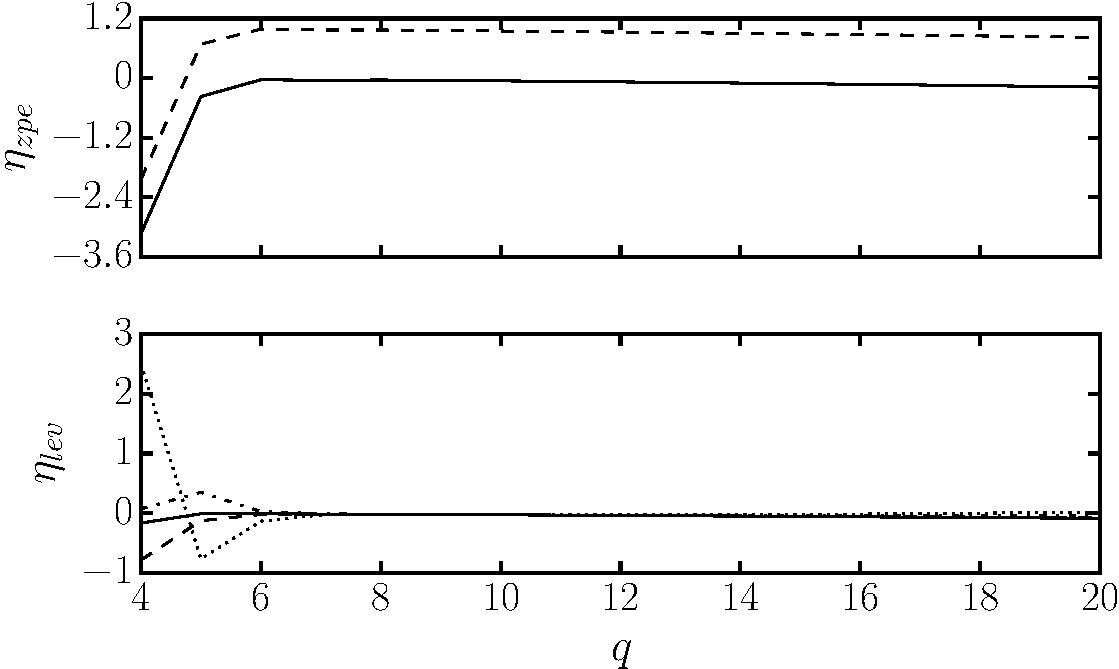
\includegraphics[width=.8\linewidth]{nonabcorr}
  % anc/scripts/nonabelian_fig.jl
  \caption{\emph{Top panel}: ``Zero-point energy" error, with (solid
curve, $\eta_{\text{zpe}}^{\text{nab}}$) and without (dashed line,
$\eta_{\text{zpe}}$) the shift from the off-diagonal matrix elements
of the Berry connection. Including just the first term in the sum
Eq.~\eqref{eq:shift} gives an identical curve to the one of
$\eta_{\text{zpe}}^{\text{nab}}$. The chosen trap strength is $\kappa
= 0.02 J$.  \emph{Bottom panel}: Level-spacing error, for the same
trap strength, considering $\beta = 0,1$ (solid curve), $\beta = 1,2$
(dashed curve), $\beta = 2,3$ (dashed-dotted curve) and $\beta = 3,4$
(dotted curve).}
  \label{fig:zpe}
\end{figure}

We turn now to the level-spacing error $\eta_{\text{lev}}$. This can
be expressed as
\begin{equation} \eta_{\text{lev}} = \frac{2\pi \alpha}{\kappa}
[E_{\text{ex}}(\beta) - E_{\text{ex}}(\beta - 1)] -1,
\end{equation} where we have used that the analytical level spacing
from Eq.~\eqref{eq:ladders} is simply $\kappa / 2\pi \alpha$.  We plot
the level-spacing error in the bottom panel of Fig.~\ref{fig:zpe} for
$\beta = 1, 2, 3$ and 4. As can be seen here, there is a large
variation in the errors at small $q$ due to the large
bandwidth~\cite{ozawa2014momhh}. On the other hand, we see that
$\eta_{\text{lev}} \ll 1$, for $q \gtrsim 6$, where the flat-band
approximation improves. In this regime, the level-spacing error is
much smaller than the zero-point error. This is because when the shift
from the off-diagonal matrix elements of the Berry connection
Eq.~\eqref{eq:shift} is approximately uniform over the MBZ at large
$q$, it just acts as a uniform energy shift on all the states in a
ladder with band index $n$. Consequently, this shift drops out of the
level spacing error between states, leaving only higher-order
band-mixing terms. From perturbation theory, it is expected that
mixing with other bands leads to a negative energy shift on states in
the lowest band, and indeed this can be seen in both
$\eta_{\text{zpe}}^{\text{nab}}$ and $\eta_{\text{lev}}$ in the small
negative errors found at large $q$.

\subsection{Driving and dissipation}\label{sec:driven-dissipation}

We now include in our model the driving and dissipation that are an
integral part of the proposed photonics experiment. We assume there
are uniform and local losses characterized by a loss rate $\gamma$,
and that the pump is monochromatic, with frequency $\omega_0$ and a
spatial profile $f_{m,n}$. Following the treatment of
Ref.~\cite{ozawa2014qhe}, we replace the bosonic creation and
annihilation operators with their expectation values, as can be
justified for a noninteracting system. The steady state evolution of
the photon-field amplitude in a cavity then follows that of the pump
as $a_{m,n}(t) = a_{m,n} e^{-i \omega_0 t}$. Combining Hamiltonian
evolution with pumping and losses, one arrives at a set of linear
coupled equations that can be solved numerically for the
steady-state\cite{cohen1992atom}:
%
\begin{multline}\label{eq:linear_problem} f_{m,n}
=J\left[e^{-i\phi_{m,n}^x}a_{m+1,n}+e^{i\phi_{m-1,n}^x}a_{m-1,n}
\right. \\
\left. +e^{-i\phi_{m,n}^y}a_{m,n+1}+e^{i\phi_{m,n-1}^y}a_{m,n-1}\right]
\\ +\left[\omega_{0}+i\gamma-\frac{1}{2}\kappa
\left((m-m_0)^{2}+(n-n_0)^{2}\right)\right]a_{m,n}
\end{multline} where we have reintroduced the position of the harmonic
trap centre $(m_0, n_0)$, although unless otherwise specified we set
$(m_0, n_0)=(0,0)$ in our simulations.

The expectation values $\abs{a_{m,n}}^2$ correspond to the number of
photons at site $(m,n)$, whereas the intensity spectrum is given by
their total sum $\sum_{m,n} |a_{m,n}|^2$ as a function of pump
frequency $\omega_0$. These observables can be directly related to the
eigenstates of the Hamiltonian in Eq.~\eqref{eq:model}. Firstly, the
different eigenmodes of a driven-dissipative system will appear as
peaks in the transmission and/or absorption spectra under a coherent
pump~\cite{carusotto2013fluids}. The resonance peaks will be broadened
by the decay rate $\gamma$, while the area of the peaks will depend on
the overlap between the spatial amplitude profile of the pump and the
underlying eigenstate of $\mathcal{H}$ at that energy.

Secondly, when the pump frequency is set on resonance with a given
mode, the intensity profiles in both real- and momentum-space
reproduce the wave function of that
mode~\cite{carusotto2013fluids}. This corresponds respectively to
measuring the near-field and far-field spatial emission of photons
from the cavity array. We note that the far-field emission is simply
the Fourier-transform of the real-space wave function and so will be a
function of crystal momentum defined in the full BZ. To reach the MBZ,
a further processing step is required; for example, if the
Harper-Hofstadter Hamiltonian is in the Landau gauge and if we choose
a magnetic unit cell of $q$ plaquettes along $\hat{x}$, the
appropriate transformation takes a particularly simple
form~\cite{price2014magnetic}:
%
\begin{equation} \label{eq:trans} \sum_n
\abs{\psi_n(\vt{p}_\mathrm{MBZ})}^2 = \sum_j
\abs{\psi(\vt{p}_\mathrm{BZ} = \vt{p}_\mathrm{MBZ}- j\vt{G})}^2 ,
\end{equation}
%
where $\psi_n(\vt{p}_\mathrm{MBZ})$ is the wave function coefficient
in the MBZ, while $\psi(\vt{p}_\mathrm{BZ})$ is that in the original
BZ. In this expression, $j$ is an integer, while $\vt{G} = (2\pi/q)
\hat{\vt{p}}_x $ is the magnetic reciprocal lattice vector, where the
factor of $q$ is due to the enlarged magnetic unit cell. We note that
for other magnetic gauges or for other choices of the magnetic unit
cell, this transformation will in general be more complicated. In this
sense, we call this choice of magnetic unit cell, a ``natural" choice
when the Harper-Hofstadter Hamiltonian is in the Landau gauge.  In the
rest of the article, we denote the momentum in the original BZ as
$\mathbf{p}$, and that in the MBZ as $\mathbf{p}^0$.

\section{Results and discussion}
\label{sec:results}

\subsection{Pumping and gauge-dependent effects}
\label{sec:selection}

\begin{figure}[tb]\centering
  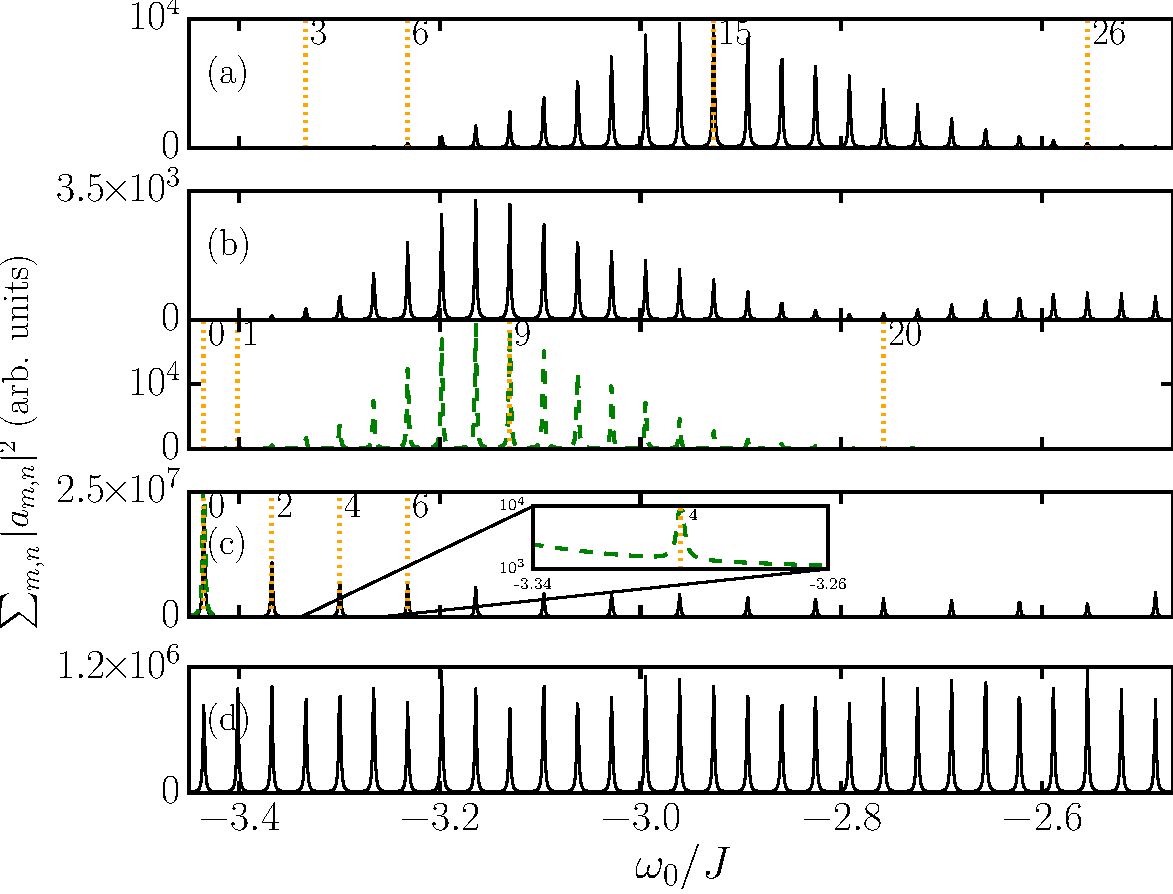
\includegraphics[width=\linewidth]{selection}
  % anc/scripts/selection_fig.jl
  \caption{Intensity spectra for different pumping conditions: (a)
pumping the single site (5,5), (b) pumping with a Gaussian profile
centered at site (5,5) with width $\sigma=1$, (c) homogeneous pumping
across all lattice sites and (d) pumping with a random phase across
all lattice sites. These results were obtained by numerical solving
Eq.~\eqref{eq:linear_problem} for the steady-state in a lattice of $N
\times N = 45 \times 45$ sites, with $\kappa = 0.02 J$, $\gamma =
0.001 J$ and $\alpha = 1/11$.  Black (solid) curves correspond to
using the Landau gauge while green (dashed) ones to the symmetric
gauge. The dotted vertical lines (with labels indicating the value of
$\beta$) mark the states which were selected for later analysis. The
spectra in panels (a) and (d) are identical for both gauges.}
  \label{fig:pumping_schemes}
\end{figure}

As introduced above, spectroscopic measurements can be used in a
driven-dissipative photonics experiment to study the trapped
Harper-Hofstadter model and hence toroidal Landau levels in momentum
space. In this section, we focus on the effects of the pumping,
exploring how different pumping schemes excite the eigenstates with
different weights. We find that such spectroscopic measurements are
sensitive to the underlying synthetic magnetic gauge chosen in a given
implementation of the Harper-Hofstadter Hamiltonian.

To best illustrate these gauge-dependent effects, we present the
results of numerically solving Eq.~\eqref{eq:linear_problem} for the
steady-state in a large lattice of $N \times N = 45 \times 45$ sites,
with $\kappa = 0.02 J$, $\gamma = 0.001 J$ and $\alpha = 1/11$.  These
parameters are chosen to highlight the key features of different
pumping schemes; we will present numerical results for a more
realistic experimental system in Section \ref{sec:experiment}.  The
numerical code was written in \textsc{Julia}~\cite{bezanson2014julia}
and is available in appendix~\ref{sec:source-code-landau}.

The intensity spectrum of the steady-state as a function of pump
frequency is shown in Fig.~\ref{fig:pumping_schemes}, where we compare
results for both the Landau and symmetric gauge for four pumping
schemes, discussed in turn below. For simplicity we limit ourselves to
pump frequencies located between the two lowest-lying
Harper-Hofstadter bands of the untrapped system. This allows us to
focus only on states within the first ladder of the trapped system
(Eq.~\eqref{eq:ladders} with $n = 0$). At higher energies, the clear
identification of states is more difficult as more than one ladder of
toroidal Landau levels can overlap, as shown, for example, in
Section~\ref{sec:experiment}.

{\em{Single-site pumping--}}The first and simplest case that we
consider is that of pumping a single site $f_{m,n} = \delta_{m,m_0}
\delta_{n,n_0}$ at an off-center lattice site. These results are shown
in Fig.~\ref{fig:pumping_schemes} panel (a), where the uniform energy
spacing of the toroidal Landau levels can be clearly observed. For
this pumping scheme, we find no significant differences between the
spectra for the Landau or symmetric gauge. This is to be expected as
changing the gauge is equivalent to changing the relative phase
between different sites, but as we are only pumping one site, this
phase difference is unimportant.

Instead, for both magnetic gauges, we see that the peak height is very
small for low energy states, rising to a maximum as energy increases,
before decreasing once more. This behaviour can be understand by
considering the form of the real space wavefunctions of $\mathcal{H}$.
In real space, the eigenstates are rings of finite width which
increase in radius as the energy increases (as can be seen in
Fig.~\ref{fig:delta_real_sp}). Analytically, we can predict how the
ring radius scales with energy by remembering that the term
$(\beta + 1/2) \kappa |\Omega_n|$ in Eq.~\eqref{eq:ladders} is the
momentum-space kinetic energy $\frac{\kappa}{2}r^2$ where
$r = i\nabla_{\mathbf{p}} + \mathcal{A}_{0, 0}(\mathbf{p})$ is the
physical position operator in the lowest band. From this, we deduce
that $r^2 \approx \frac{1}{\pi} q \beta$, as can be confirmed
numerically. Therefore, if one pumps an off-center site, there will
only be a limited range of rings that will have radii that will
overlap with the pump spot and so be excited. Here, we have set the
pump spot to be at position $(5,5)$, and from the above scaling, the
toroidal Landau level that best overlaps with this pump will have a
quantum number $\beta \approx 14$, which is in good agreement with the
numerical results shown in Fig.~\ref{fig:pumping_schemes} (a).

\begin{figure}[tb] \centering
  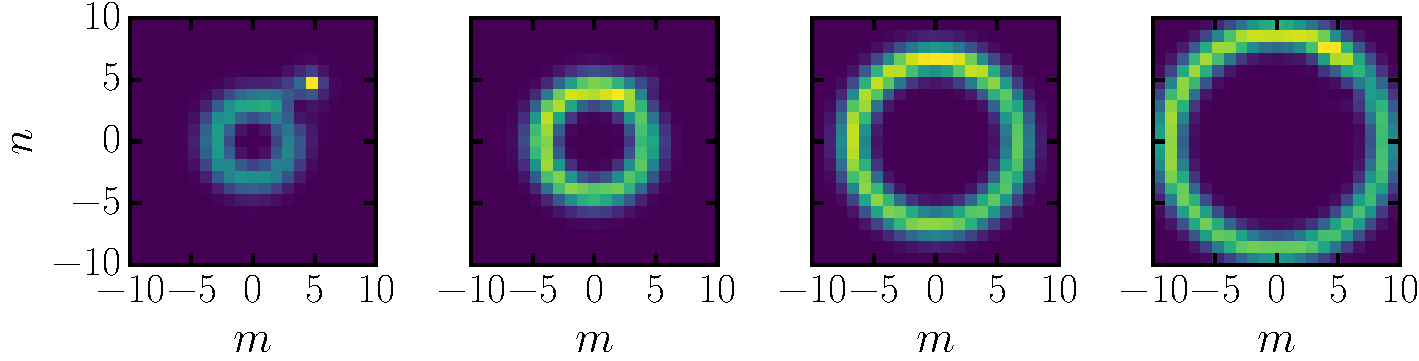
\includegraphics[width=0.9\linewidth]{real}
  % anc/scripts/selection_fig.jl
  \caption{Real space reconstruction of the states $\beta=3$, 6, 15
and 26 of Fig.~\ref{fig:pumping_schemes}(a).}
  \label{fig:delta_real_sp}
\end{figure}

{\em{Gaussian pumping--}} We now consider a Gaussian pump as the next
logical step up in complexity from a single-site pump. This has the
form $f_{m,n} = \exp- \frac{1}{2\sigma^2} \left[(m-m')^2 + (n-n')^2
\right]$, and we choose $\sigma =1$ and for the pump centre to be at
$(m',n') = (5,5)$, as for single-site pumping. The results are shown
in Fig.~\ref{fig:pumping_schemes} (b). The main effect is, as
expected, that more states become visible in both the low- (smaller
$\beta$) and high-energy (larger $\beta$) sections of the
spectrum. This is because the pump has a greater spatial width and so
overlaps with a larger range of real-space eigenstates.

However, we can also see that the intensity spectrum now depends on
the underlying magnetic gauge, as the phase of the eigenstates is
important. In particular, more high-energy peaks can be seen for the
Landau gauge than for the symmetric gauge. This can be most easily
understood by noting that in momentum space, the symmetric-gauge
states also have a ring-like structure (see bottom panel of
Fig.~\ref{fig:hom_mom_sp}), where the ring radius increases with
$\beta$. To see this, we note that, in the symmetric gauge, the
real-space wavefunctions have a phase which winds around the ring as
$e^{i\beta \phi}$ where $\phi$ is the polar angle around the
ring. This phase-winding sets the radius of the rings in momentum
space as $p^2 \approx \pi \frac{\beta}{q}$; a scaling that can be
confirmed numerically and seen in Fig.~\ref{fig:hom_mom_sp}, bottom
panel. (The white spot close to the edges of the rings in these
figures is due to destructive interference with the pump.)  As the
Fourier transform of the Gaussian pump is again a Gaussian, it follows
that only a limited range of low-energy symmetric-gauge momentum-space
states will have a good overlap with the pump. The high energy portion
of the spectrum is therefore washed out compared to its Landau gauge
counterpart, where states have higher amplitude close to the centre of
the BZ and so better overlap with the pump.

\begin{figure}[tb]\centering
  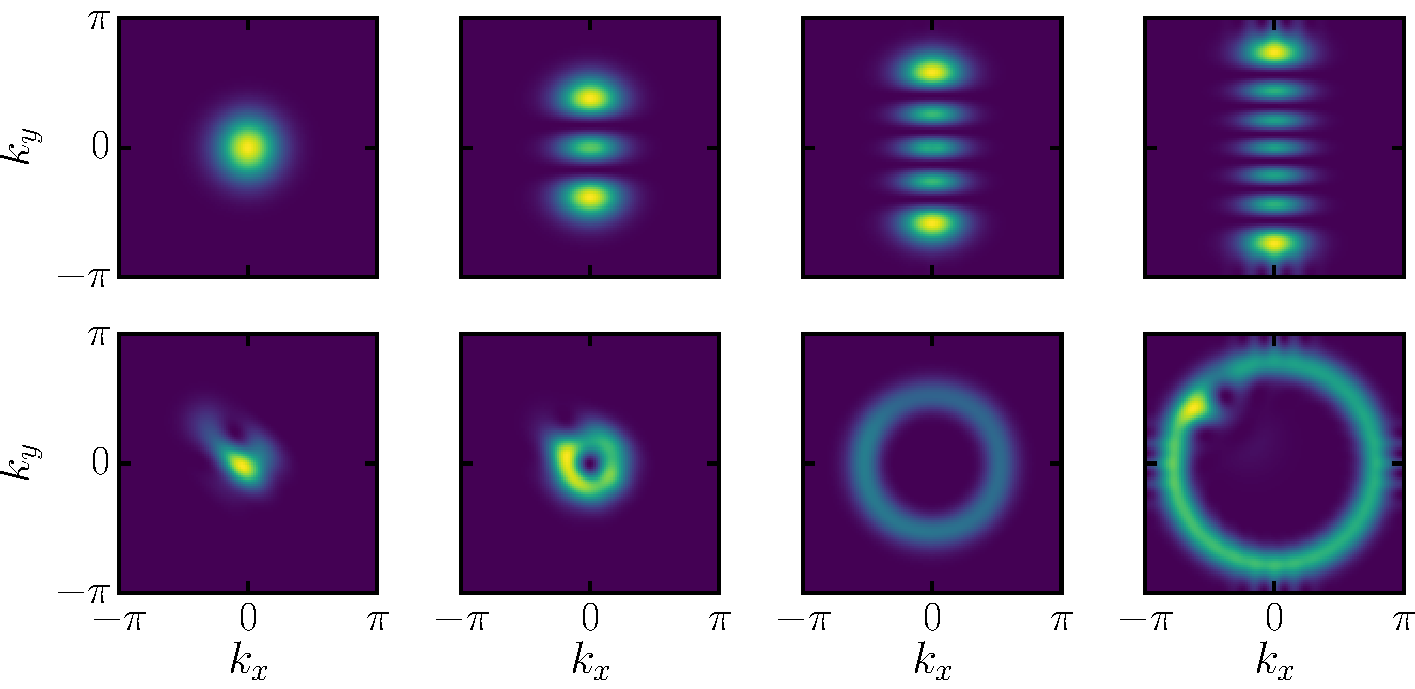
\includegraphics[width=0.9\linewidth]{momentum}
  % anc/scripts/selection_fig.jl
  \caption{Momentum space reconstruction of the eigenstates. \emph{Top
row}: states corresponding to $\beta=0$, 2, 4 and 6 in
Fig.~\ref{fig:pumping_schemes}(c), using the Landau gauge.
\emph{Bottom row}: states corresponding to $\beta=0$, 1, 9 and 20 in
Fig.~\ref{fig:pumping_schemes}(b), using the symmetric gauge.}
  \label{fig:hom_mom_sp}
\end{figure}

Before continuing, we also note that for sufficiently large values of
$\beta$ the symmetric-gauge rings in momentum space will increase to
the point where they touch the BZ boundaries. When this occurs,
self-interference patterns appear in the wave function as shown for
example in Fig.~\ref{fig:torus_edge}. The extra ring-like structures
appearing for $\beta \geq 30$ in Fig.~\ref{fig:torus_edge} are due to
the close proximity of states pertaining to other ladders with $n
>0$. Note that in order to excite such high-energy states, we have
used a pump with a homogeneous amplitude and a random onsite phase, as
will be presented in the fourth pumping case below.

{\em{Homogeneous pumping with uniform phase--}} If we now take the
limit of a very wide Gaussian, we reach a homogeneous pump profile
extended over all lattice sites. The results for this pumping scheme
are shown in panel (c) of Fig.~\ref{fig:pumping_schemes}. Now $f_{m,n}
= f$, and we see that the intensity spectrum is strongly
magnetic-gauge dependent. In the Landau gauge, firstly, there are
visible peaks for only half of the states. This can be understood by
noting that a homogeneous pump in real space is a $\delta$ function in
momentum space centered in the middle of the BZ. If we consider the
Landau-gauge eigenstates in the full BZ, as shown in the top row of
Fig.~\ref{fig:hom_mom_sp}, we see that the states with an even value
of $\beta$ have an even number of nodes, with a lobe at the BZ
center. Conversely, the states with odd values of $\beta$ have an odd
number of nodes, including one at the BZ center. (These feature can be
related back to the properties of the Hermite polynomials in the
analytical eigenstates in the MBZ Eq.~\eqref{eq:chi}.) Consequently,
only states with even values of $\beta$ have a good overlap with the
pump, and the intensity spectrum contains half the expected peaks, now
separated by twice the toroidal Landau level energy spacing.

In the symmetric gauge, secondly, we find only one out of every four
states for homogeneous pumping, as can be seen in the inset of
Fig.~\ref{fig:pumping_schemes} (c). This is due to the fact that, on a
square lattice, the angular momentum is conserved modulo 4, respecting
the 4-fold rotational symmetry. The peak intensity gets smaller for
larger $\beta$ because of the diminishing overlap of the localized
central pump with the increasing momentum-space ring discussed above.

\begin{figure}[tb] \centering
  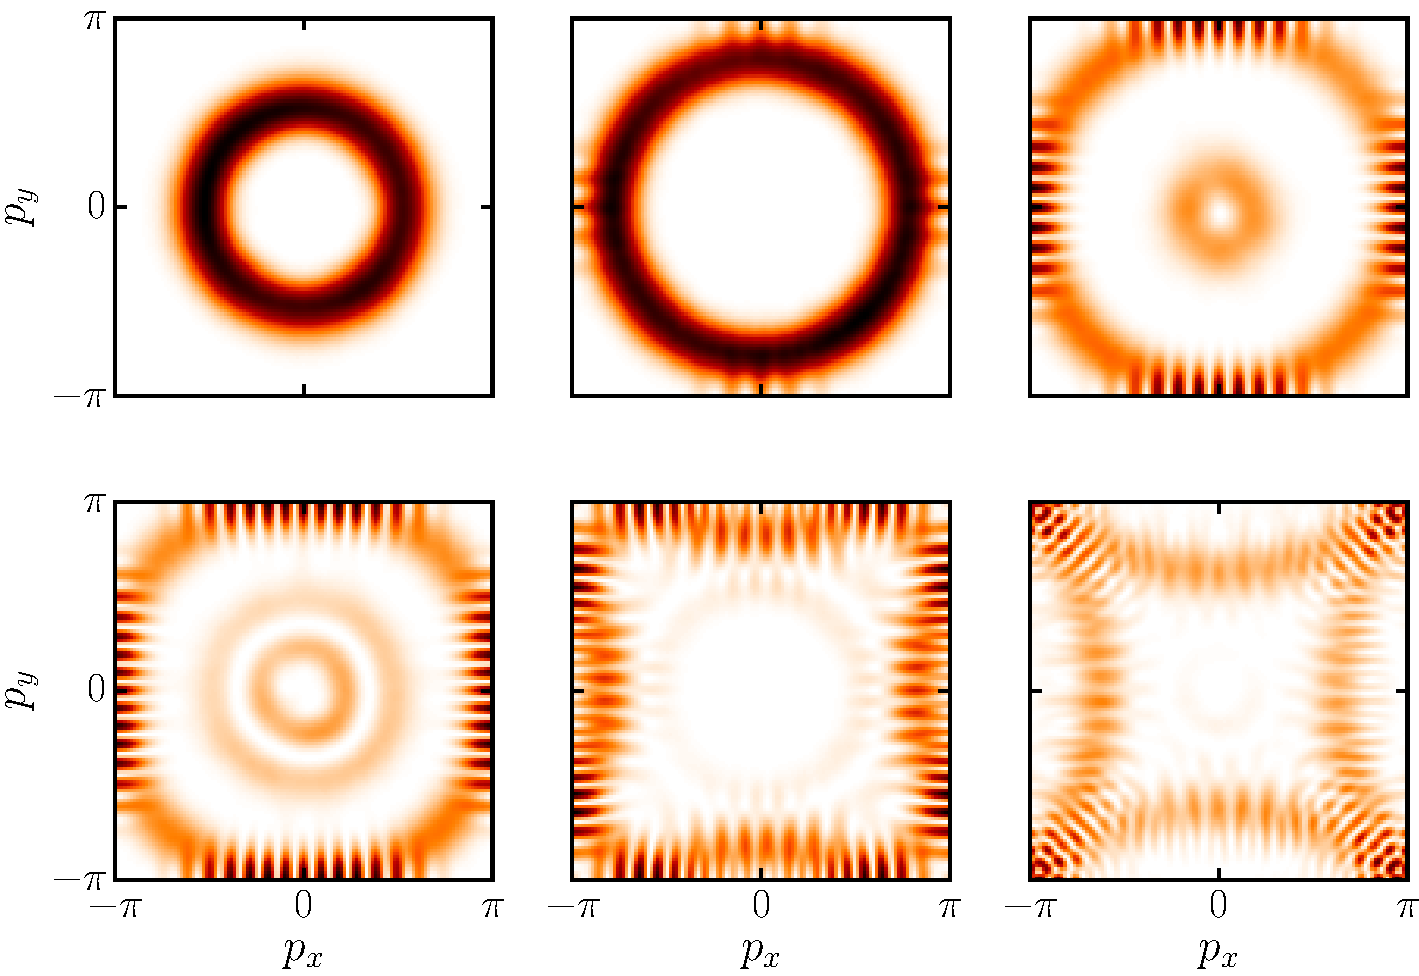
\includegraphics[width=.7\linewidth]{sym_ring}
  % anc/scripts/torus_edge_fig.jl
  \caption{Momentum space reconstruction of the eigenstates in the
full BZ, using the symmetric gauge and homogeneous pumping with a
random on-site phase. \emph{Top row}: states corresponding to $\beta =
9, 20, 30$.  \emph{Bottom row}: states corresponding to $\beta = 38,
59, 99$. Parameters are the same as in
Fig.~\ref{fig:pumping_schemes}.}
  \label{fig:torus_edge}
\end{figure}


{\em{Homogeneous pumping with a random on-site phase --}} As the
fourth scheme, we consider a pump with a uniform amplitude over the
lattice but a random site-dependent phase $\phi_{m,n}$:
$f_{m,n}=fe^{i\phi_{m,n}}$. The phases are chosen from a random
uniform distribution, and have values in the interval $[0,2\pi)$. The
bottom panel of Fig.~\ref{fig:pumping_schemes} was obtained by
averaging over 100 distinct realizations of these random phases. This
results in a relatively even intensity distribution, for both gauges,
where we can associate a peak to each toroidal Landau level in this
energy window. While such a pumping scheme would therefore be the best
way to excite all the eigenstates and to fully probe the
momentum-space physics, we note that this would also be difficult to
achieve in an experiment.
%
\begin{figure}[htb] \centering
  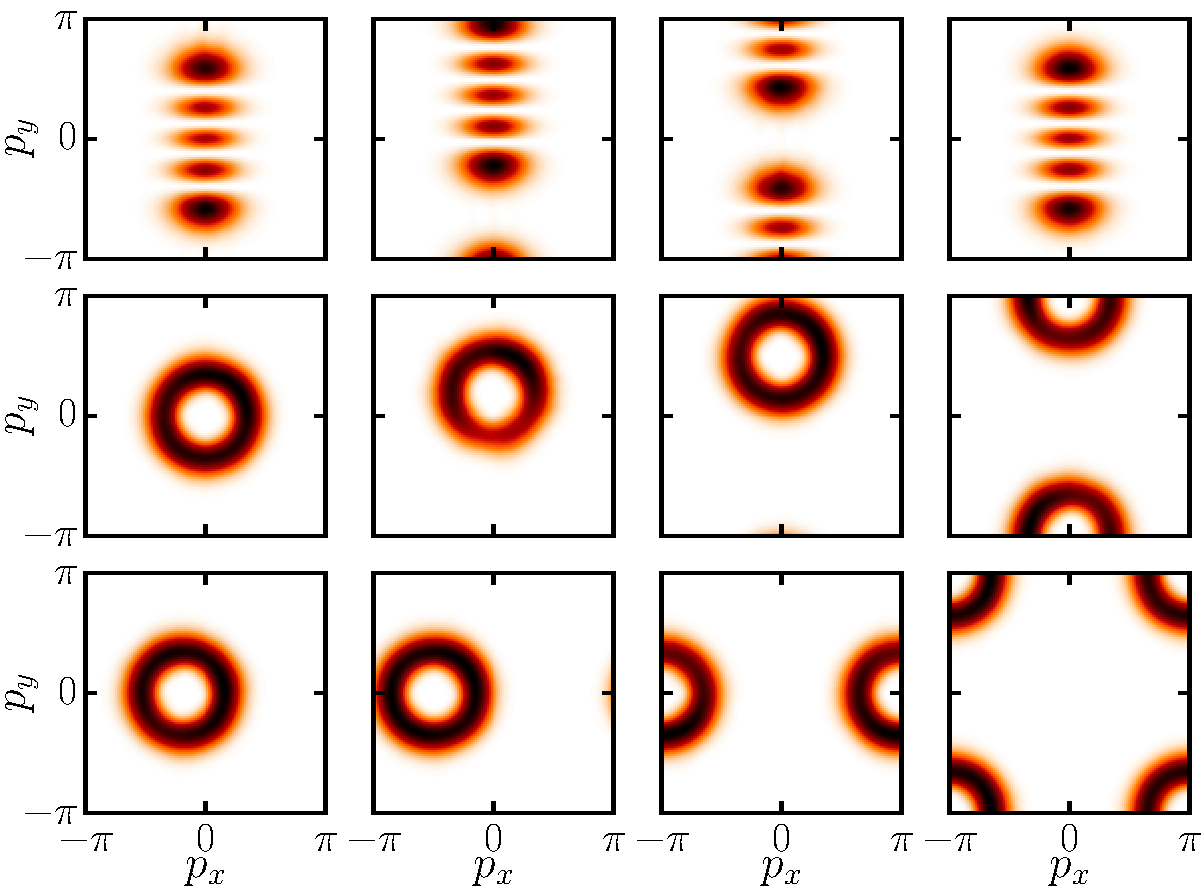
\includegraphics[width=.8\linewidth]{fringe_trap}
  % anc/scripts/torus_edge_fig.jl
  \caption{Momentum space reconstruction of the eigenstates in the
full BZ, using the Landau (top row) and symmetric gauge (middle and
bottom row) and a spatially homogeneous pump with a random on-site
phase. We have considered the state $\beta = 4$ for different trap
positions $(m_0, n_0)$. For the top and middle rows, we have (from
left to right): (0,0) (trap in the center), (2,0), (5.5,0) and (11,0),
whereas for the bottom row we chose the positions (0,2), (0,5.5),
(0,11) and (11,11). Parameters are the same as in
Fig.~\ref{fig:pumping_schemes}.}
  \label{fig:moving_trap}
\end{figure}
%
\begin{figure}[htb] \centering
  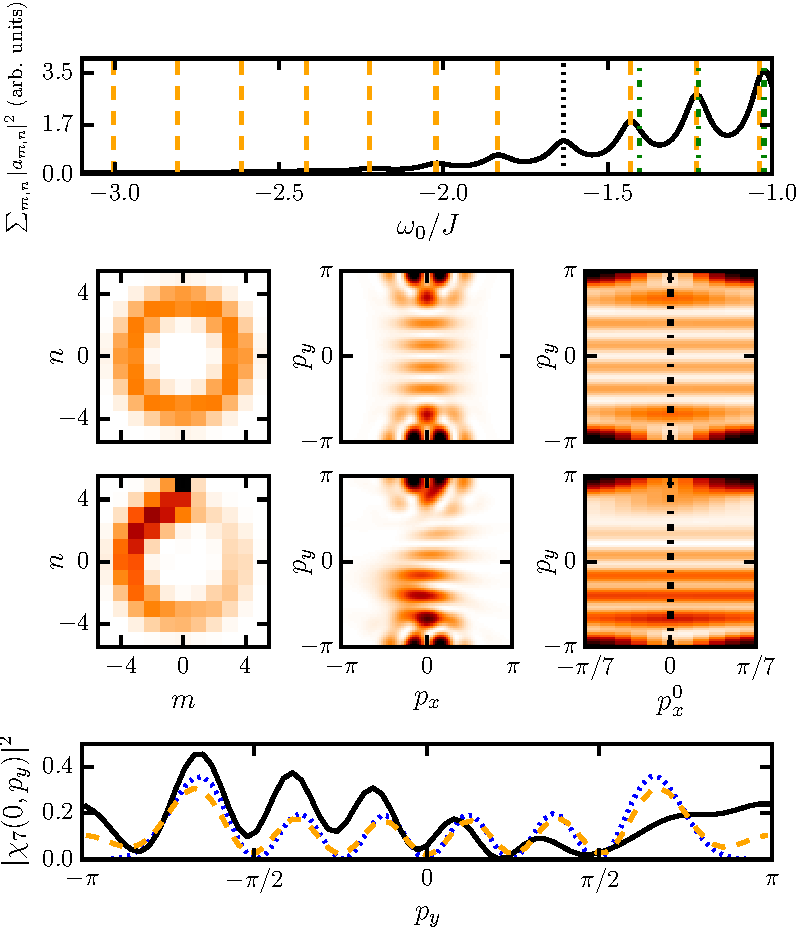
\includegraphics[width=.7\linewidth]{exp_fig}
  % anc/scripts/experimental_fig.jl
  \caption{\emph{Top row}: Intensity spectrum for a small lattice of
    $11 \times 11$ sites, with $\gamma = 0.05 J$, $\kappa = 0.2 J$ and
    $\alpha=1/7$.  \emph{Second row}: Profile of the $\beta=7$ state
    in real space (left), momentum space (center) and the population
    over bands in the MBZ (right) for the conservative system.
    \emph{Third row}: Reconstruction of the $\beta=7$ mode
    wavefunction in real space (left), momentum space (center) and the
    population over bands in the MBZ (right) obtained in the
    driven-dissipative system by pumping at $\omega_0 = -1.63 J$, on
    resonance with the desired mode (black dotted line in the top
    panel).  The $\delta$-like pump at (0,5) is visible as a dark
    square in the left panel.  \emph{Bottom row}: Slice along the
    $p_x^0 = 0$ line in the MBZ (solid black line), compared to the
    analytical prediction of Eq.~\eqref{eq:chi}, $|\chi_7(0,p_y)|^2$
    (blue dotted line) and to the population over bands for the
    nondissipative system (dashed orange line).}
  \label{fig:exp}
\end{figure}

Before continuing, we give a final example of an interesting
gauge-dependent effect that could be studied experimentally in this
system. Unlike the physics discussed above, this is not directly
related to the pumping but instead to the behaviour of the wave
function under a change in the centre of the harmonic trap $(m_0,
n_0)$. As derived in Ref. ~\cite{ozawa2014momhh}, moving the harmonic
trap in space changes the boundary conditions on the wave function in
the MBZ. We note that although this derivation was made explicitly for
the magnetic Landau gauge in the MBZ, numerically we observe here that
this physics is also seen in the full BZ in both gauges.  As shown
in Fig.~\ref{fig:moving_trap}, a shift in the harmonic trap centre in
one direction shifts the observed momentum-space pattern in the
perpendicular direction. This behaviour can be understood as a
realisation of Laughlin's {\em Gedankenexperiment} for the quantum
Hall effect but now in momentum space~\cite{ozawa2014momhh}. As we
observe, the momentum-space wave function returns to itself after the
harmonic trap has been moved $q$ lattice sites for the magnetic Landau
gauge but $2q$ lattice sites for the magnetic symmetric gauge,
reflecting the underlying translational symmetry of $\mathcal{H}_0$ in
the two different gauges.


\subsection{Results for realistic experimental parameters}
\label{sec:experiment}

We now present numerical results for system parameters within current
experimental reach, to demonstrate that the essential characteristics
of toroidal Landau levels could be probed experimentally for the first
time in photonics. We choose a small lattice of only $11 \times 11$
sites, with losses of $\gamma = 0.05 J$; this loss rate is in the same
range as those present in the experiment of
Ref.~\cite{hafezi2013imaging}. Such a large loss rate broadens the
peaks in the intensity spectrum, making closely-spaced eigenenergies
harder to resolve. From Eq.~\eqref{eq:ladders}, we see that the level
spacing is given by $\frac{\kappa}{2\pi\alpha}$, and so we can
increase the energy spacing by applying a stronger harmonic potential,
chosen here as $\kappa = 0.2 J$. Increasing the strength of the
harmonic trap improves our flat-band approximation, but weakens the
single-band approximation. To compensate for this, we consider a
larger value of $\alpha = 1/7$, for which the larger band-gap $(E_1 -
E_0)$ reduces band-mixing effects.

As in the experiment of Ref.~\cite{hafezi2013imaging}, we work in the
Landau gauge for the Harper-Hofstadter Hamiltonian, with hopping
phases given by $\phi = (0, 2\pi\alpha m)$. In order to model the
experimental pumping scheme where light was injected into a single
resonator at the edge of the system via an external integrated
waveguide~\cite{hafezi2013imaging}, we consider a localized pump on a
single site situated on the upper border of the system at
$(m_0,n_0)= (0,5)$.  The corresponding intensity spectrum is shown in
the 1st row of Fig.~\ref{fig:exp}. Apart from the expected broadening
due to larger losses, the peaks observed correspond well to the
expected eigenenergies.  As discussed above, single-site pumping
limits the number of visible peaks, as the heights of the peaks at
low-energies are suppressed due to the poor overlap of the real-space
eigenstate with the pump position. However, as this pumping scheme is
closest to that used in experiments, we emphasise that even in this
case, enough peaks can be observed to extract quantitative
measurements of the toroidal Landau level spacing. The orange vertical
(dashed) lines show the first ladder of eigenstates of $\mathcal{H}$
from Eq.~\eqref{eq:model}. We also note that here for frequencies
larger than $-1.5 J$, we also start to see states from the second
ladder $\epsilon_{1,\beta}$ (see Eq.~\eqref{eq:ladders}), which are
depicted as green vertical dash-dotted lines. Their proximity to the
first ladder states means they cannot be easily resolved as separate
peaks in the dissipative spectrum.

Setting the pump frequency at the energy indicated by the black dotted
line, we plot the numerical near- and far-field emission in the left
and center panels of the 3rd row of Fig.~\ref{fig:exp}. This
corresponds to the wave function in real space and in the full BZ,
respectively. By applying the transformation in Eq.~\eqref{eq:trans}, we
can also map the wave function in the full BZ to the population over
bands in the MBZ, as shown in the right panel of the 3rd row of
Fig.~\ref{fig:exp}. For comparison, we plot these quantities for the
corresponding numerical eigenstate of $\mathcal{H}$
Eq.~\eqref{eq:model} in the second row of Fig.~\ref{fig:exp}, for
which there is no pumping and dissipation.

We find very good qualitative agreement between the numerical results
in the MBZ and the analytical toroidal Landau level Eq.~\eqref{eq:chi}
with $\beta=7$, as expected. We can make a quantitative comparison with
this analytical eigenstate by taking a slice along the dash-dotted
vertical lines ($p_x^0 = 0$) in the right column of rows 2 and 3;
these cuts are shown in the bottom panel of Fig.~\ref{fig:exp} along
with a dotted blue curve indicating the analytical eigenstate. As can
be seen, there is excellent agreement between the numerics without
driving and dissipation and the analytical result. We have checked
that reducing $\kappa$ makes this fit even better, pointing towards
band-mixing effects. Introducing pumping and dissipation distorts the
eigenstate, but many characteristic features are still clearly
observable.

It is particularly interesting to note that in the driven-dissipative
steady-state in real space, shown in the left panel of the 3rd row of
Fig.~\ref{fig:exp}, the photon distribution breaks the rotational
symmetry of the ring eigenstate. While this can be physically
understood as a decaying cyclotron orbit with an inverse lifetime set
by $\gamma$, in terms of eigenmodes the exponential decay (and more
generally the breaking of the rotational symmetry) results from the
interference of several modes which overlap in frequency due to the
relatively large value of $\gamma$.  In the same way that real-space
Landau levels give rise to real-space cyclotron orbits under the
effect of the magnetic field, the observation of momentum-space Landau
levels can provide clear evidence of a cyclotron orbit in momentum
space under the effect of the Berry curvature, whose effect is indeed
that of a momentum-space magnetic field.

Finally, we briefly summarize how one can practically measure the
contribution $\delta E_0$ from the off-diagonal matrix elements of the
Berry connection (see Eq.~\eqref{eq:shift}) from the intensity
spectrum. Starting from an experimental spectrum, one first needs to
select a particular peak and determine its $\beta$ label by comparing
the MBZ reconstruction with the analytical result. The distance
between two neighbouring peaks gives the level spacing $\kappa
\abs{\Omega_0}$. Finally, to separate the shift $\delta E_0$ from the
Harper-Hofstadter ground state energy $E_0$ in Eq.~\eqref{eq:ladders},
one can make use of the fact that the former depends on the trap
strength $\kappa$, while the latter does not. Preparing two otherwise
identical samples with different trap strengths and subtracting the
ground state energy will then allow for a direct measurement of the
contribution from the off-diagonal matrix elements of the Berry
connection.

\section{Conclusion}
\label{sec:conclusion}

In conclusion, we have shown that the observation of toroidal Landau
levels in momentum space is within experimental reach for
state-of-the-art driven-dissipative photonic systems. Our proposal
combines the recent realisation of the Harper-Hofstatder model in an
array of silicon-based coupled ring resonators in
Ref.~\cite{hafezi2013imaging}, with a harmonic potential, which could
be introduced through a spatial modulation of the resonator size. We
have presented numerical results to show that even for very small
lattices, in the presence of driving and strong dissipation, key
characteristics of the toroidal Landau levels can still be
extracted. This would be a first direct investigation of analogue
magnetic eigenstates in momentum space.

We have also emphasised that the proposed photonics experiment would
be able to highlight a momentum-space analog of the cyclotron motion
as well as to measure the energy shift due to the off-diagonal matrix
elements of the Berry connection, which, as these are inter-band
geometrical properties, are hard to access by other means. We have
also discussed how the spectroscopic measurements presented here are
sensitive to the specific synthetic magnetic gauge implemented in an
experiment.

Finally, an interesting outlook would be to include the effect of
photon-photon interactions in the model, as the degenerate ground
states predicted in~\cite{ozawa2014momhh} for a weakly-interacting
trapped Harper-Hofstadter model may lead to interesting nonlinear
dynamical features. In the longer run, when the synthetic gauge field
is combined with strong interactions, one can hope to observe the
hallmarks of fractional quantum Hall
physics~\cite{umucalilar2012fractional,hafezi2013non}.

\begin{subappendices}

  \section{Source code}\label{sec:source-code-landau}
  %
  This appendix contains \textsc{Julia} 0.3 source code for the
numerical simulations used to produce the figures appearing in
Chapter~\ref{cha:landau}. Sec.~\ref{subsec:bp} contains the main
program module, defining the functions used in simulations, while
Sec.~\ref{subsec:hh} contains the module for constructing and
diagonalizing the Harper-Hofstadter Hamiltonian.
  %
The figures are plotted using the \textsc{matplotlib} \textsc{Python}
library v1.4.3, as follows: Sec.~\ref{subsec:nonabelian} contains the
code for Fig.~\ref{fig:zpe}; Sec.~\ref{subsec:selection} produces
Figs.~\ref{fig:pumping_schemes}, \ref{fig:delta_real_sp},
and~\ref{fig:hom_mom_sp}; Sec.~\ref{subsec:torus-edge} produces
Figs.\ref{fig:torus_edge} and~\ref{fig:moving_trap} and finally,
Sec.~\ref{subsec:experimental} produces Fig.~\ref{fig:exp}.
  %
  %%%%%%%%%%%%%%%%%%%%%%%%%%%%%%%%%%%%%%%%%%%%%%%%%
% pygmentize -l julia -f latex -o BP.tex BP.jl  %
%%%%%%%%%%%%%%%%%%%%%%%%%%%%%%%%%%%%%%%%%%%%%%%%%

\subsection{BP.jl}\label{subsec:bp}
\begin{Verbatim}[commandchars=\\\{\}]
\PY{k}{module} \PY{n}{BP}
\PY{k}{using} \PY{n}{Polynomials}
\PY{k}{using} \PY{n}{Base}\PY{o}{.}\PY{n}{Test}
\PY{k}{type}\PY{n+nc}{ }\PY{n+nc}{WaveFunction}
    \PY{n}{N}\PY{p}{:}\PY{p}{:}\PY{k+kt}{Int}
    \PY{n}{int}\PY{p}{:}\PY{p}{:}\PY{k+kt}{Float64}
    \PY{n}{ψ}\PY{p}{:}\PY{p}{:}\PY{n}{Vector}\PY{p}{\PYZob{}}\PY{n}{Complex}\PY{p}{\PYZob{}}\PY{k+kt}{Float64}\PY{p}{\PYZcb{}}\PY{p}{\PYZcb{}}
\PY{k}{end}
\PY{n}{WaveFunction}\PY{p}{(}\PY{n}{S}\PY{p}{:}\PY{p}{:}\PY{n}{SparseMatrixCSC}\PY{p}{\PYZob{}}\PY{n}{Complex}\PY{p}{\PYZob{}}\PY{k+kt}{Float64}\PY{p}{\PYZcb{}}\PY{p}{,}\PY{k+kt}{Int64}\PY{p}{\PYZcb{}}\PY{p}{,}
             \PY{n}{ω}\PY{p}{:}\PY{p}{:}\PY{k+kt}{Float64}\PY{p}{,}\PY{n}{P}\PY{p}{:}\PY{p}{:}\PY{n}{Vector}\PY{p}{\PYZob{}}\PY{n}{Complex}\PY{p}{\PYZob{}}\PY{k+kt}{Float64}\PY{p}{\PYZcb{}}\PY{p}{\PYZcb{}}\PY{p}{)} \PY{o}{=}
                \PY{n}{WaveFunction}\PY{p}{(}\PY{n}{S}\PY{p}{,}\PY{n}{ω}\PY{p}{,}\PY{n}{P}\PY{p}{,}\PY{p}{:}\PY{n}{landau}\PY{p}{)}
\PY{n}{WaveFunction}\PY{p}{(}\PY{n}{S}\PY{p}{:}\PY{p}{:}\PY{n}{SparseMatrixCSC}\PY{p}{\PYZob{}}\PY{n}{Complex}\PY{p}{\PYZob{}}\PY{k+kt}{Float64}\PY{p}{\PYZcb{}}\PY{p}{,}\PY{k+kt}{Int64}\PY{p}{\PYZcb{}}\PY{p}{,}
             \PY{n}{ω}\PY{p}{:}\PY{p}{:}\PY{k+kt}{Float64}\PY{p}{,}\PY{n}{P}\PY{p}{:}\PY{p}{:}\PY{n}{Vector}\PY{p}{\PYZob{}}\PY{n}{Complex}\PY{p}{\PYZob{}}\PY{k+kt}{Float64}\PY{p}{\PYZcb{}}\PY{p}{\PYZcb{}}\PY{p}{,}\PY{n}{gauge}\PY{p}{:}\PY{p}{:}\PY{n}{Symbol}\PY{p}{)}
                 \PY{o}{=} \PY{n}{WaveFunction}\PY{p}{(}\PY{n}{S}\PY{p}{,}\PY{n}{ω}\PY{p}{,}\PY{n}{P}\PY{p}{,}\PY{n}{gauge}\PY{p}{,}\PY{l+m+mi}{1}\PY{o}{/}\PY{l+m+mi}{11}\PY{p}{,}\PY{l+m+mf}{0.001}\PY{p}{,}\PY{l+m+mf}{0.02}\PY{p}{,}\PY{l+m+mf}{0.}\PY{p}{,}\PY{l+m+mf}{0.}\PY{p}{)}
\PY{n}{WaveFunction}\PY{p}{(}\PY{n}{S}\PY{p}{:}\PY{p}{:}\PY{n}{SparseMatrixCSC}\PY{p}{\PYZob{}}\PY{n}{Complex}\PY{p}{\PYZob{}}\PY{k+kt}{Float64}\PY{p}{\PYZcb{}}\PY{p}{,}\PY{k+kt}{Int64}\PY{p}{\PYZcb{}}\PY{p}{,}
             \PY{n}{ω}\PY{p}{:}\PY{p}{:}\PY{k+kt}{Float64}\PY{p}{,}\PY{n}{P}\PY{p}{:}\PY{p}{:}\PY{n}{Vector}\PY{p}{\PYZob{}}\PY{n}{Complex}\PY{p}{\PYZob{}}\PY{k+kt}{Float64}\PY{p}{\PYZcb{}}\PY{p}{\PYZcb{}}\PY{p}{,}\PY{n}{gauge}\PY{p}{:}\PY{p}{:}\PY{n}{Symbol}\PY{p}{,}
             \PY{n}{α}\PY{p}{:}\PY{p}{:}\PY{k+kt}{Float64}\PY{p}{,}\PY{n}{γ}\PY{p}{:}\PY{p}{:}\PY{k+kt}{Float64}\PY{p}{,}\PY{n}{κ}\PY{p}{:}\PY{p}{:}\PY{k+kt}{Float64}\PY{p}{)} \PY{o}{=}
                 \PY{n}{WaveFunction}\PY{p}{(}\PY{n}{S}\PY{p}{,}\PY{n}{ω}\PY{p}{,}\PY{n}{P}\PY{p}{,}\PY{n}{gauge}\PY{p}{,}\PY{n}{α}\PY{p}{,}\PY{n}{γ}\PY{p}{,}\PY{n}{κ}\PY{p}{,} \PY{l+m+mf}{0.}\PY{p}{,} \PY{l+m+mf}{0.}\PY{p}{)}
\PY{k}{function}\PY{n+nf}{ }\PY{n+nf}{WaveFunction}\PY{p}{(}\PY{n}{S}\PY{p}{:}\PY{p}{:}\PY{n}{SparseMatrixCSC}\PY{p}{\PYZob{}}\PY{n}{Complex}\PY{p}{\PYZob{}}\PY{k+kt}{Float64}\PY{p}{\PYZcb{}}\PY{p}{,}\PY{k+kt}{Int64}\PY{p}{\PYZcb{}}\PY{p}{,}
                      \PY{n}{ω}\PY{p}{:}\PY{p}{:}\PY{k+kt}{Float64}\PY{p}{,}\PY{n}{P}\PY{p}{:}\PY{p}{:}\PY{n}{Vector}\PY{p}{\PYZob{}}\PY{n}{Complex}\PY{p}{\PYZob{}}\PY{k+kt}{Float64}\PY{p}{\PYZcb{}}\PY{p}{\PYZcb{}}\PY{p}{,}
                      \PY{n}{gauge}\PY{p}{:}\PY{p}{:}\PY{n}{Symbol}\PY{p}{,} \PY{n}{α}\PY{p}{:}\PY{p}{:}\PY{k+kt}{Float64}\PY{p}{,}\PY{n}{γ}\PY{p}{:}\PY{p}{:}\PY{k+kt}{Float64}\PY{p}{,}
                      \PY{n}{κ}\PY{p}{:}\PY{p}{:}\PY{k+kt}{Float64}\PY{p}{,} \PY{n}{m₀}\PY{p}{:}\PY{p}{:}\PY{k+kt}{Float64}\PY{p}{,} \PY{n}{n₀}\PY{p}{:}\PY{p}{:}\PY{k+kt}{Float64}\PY{p}{)}
    \PY{n}{N}\PY{p}{:}\PY{p}{:}\PY{k+kt}{Int} \PY{o}{=} \PY{n}{sqrt}\PY{p}{(}\PY{n}{length}\PY{p}{(}\PY{n}{P}\PY{p}{)}\PY{p}{)}
    \PY{n}{eval}\PY{p}{(}\PY{p}{:}\PY{p}{(}\PY{o}{\PYZdl{}}\PY{p}{(}\PY{n}{symbol}\PY{p}{(}\PY{n}{string}\PY{p}{(}\PY{l+s}{\PYZdq{}}\PY{l+s}{buildham\PYZus{}}\PY{l+s}{\PYZdq{}}\PY{p}{,} \PY{n}{gauge}\PY{p}{,} \PY{l+s}{\PYZdq{}}\PY{l+s}{!}\PY{l+s}{\PYZdq{}}\PY{p}{)}\PY{p}{)}\PY{p}{)}\PY{p}{)}\PY{p}{)}\PY{p}{(}\PY{n}{S}\PY{p}{,} \PY{n}{N}\PY{p}{,}\PY{n}{α}\PY{p}{,}\PY{n}{κ}\PY{p}{,}\PY{n}{γ}\PY{p}{,}
       \PY{n}{ω}\PY{p}{,}\PY{n}{m₀}\PY{p}{,}\PY{n}{n₀}\PY{p}{)}
    \PY{n}{X} \PY{o}{=} \PY{n}{S}\PYZbs{}\PY{n}{P}
    \PY{k}{return} \PY{n}{WaveFunction}\PY{p}{(}\PY{n}{N}\PY{p}{,}\PY{n}{sum}\PY{p}{(}\PY{n}{abs2}\PY{p}{(}\PY{n}{X}\PY{p}{)}\PY{p}{)}\PY{p}{,}\PY{n}{X}\PY{p}{)}
\PY{k}{end}
\PY{k}{type}\PY{n+nc}{ }\PY{n+nc}{ExactStates}
    \PY{n}{N}\PY{p}{:}\PY{p}{:}\PY{k+kt}{Int}
    \PY{n}{gauge}\PY{p}{:}\PY{p}{:}\PY{n}{Symbol}
    \PY{n}{νs}\PY{p}{:}\PY{p}{:}\PY{n}{Vector}\PY{p}{\PYZob{}}\PY{k+kt}{Float64}\PY{p}{\PYZcb{}}
    \PY{n}{states}\PY{p}{:}\PY{p}{:}\PY{n}{Matrix}\PY{p}{\PYZob{}}\PY{n}{Complex}\PY{p}{\PYZob{}}\PY{k+kt}{Float64}\PY{p}{\PYZcb{}}\PY{p}{\PYZcb{}}
\PY{k}{end}
\PY{n}{ExactStates}\PY{p}{(}\PY{n}{nev}\PY{p}{:}\PY{p}{:}\PY{k+kt}{Int}\PY{p}{,} \PY{n}{gauge}\PY{p}{:}\PY{p}{:}\PY{n}{Symbol}\PY{p}{)} \PY{o}{=} \PY{n}{ExactStates}\PY{p}{(}\PY{n}{nev}\PY{p}{,} \PY{n}{gauge}\PY{p}{,} \PY{l+m+mi}{45}\PY{p}{)}
\PY{n}{ExactStates}\PY{p}{(}\PY{n}{nev}\PY{p}{:}\PY{p}{:}\PY{k+kt}{Int}\PY{p}{,} \PY{n}{gauge}\PY{p}{:}\PY{p}{:}\PY{n}{Symbol}\PY{p}{,} \PY{n}{N}\PY{p}{:}\PY{p}{:}\PY{k+kt}{Int}\PY{p}{)} \PY{o}{=} \PY{n}{ExactStates}\PY{p}{(}\PY{n}{nev}\PY{p}{,}
   \PY{n}{gauge}\PY{p}{,} \PY{n}{N}\PY{p}{,} \PY{l+m+mi}{1}\PY{o}{/}\PY{l+m+mi}{11}\PY{p}{,} \PY{l+m+mf}{0.02}\PY{p}{,} \PY{l+m+mf}{0.}\PY{p}{,} \PY{l+m+mf}{0.}\PY{p}{)}
\PY{n}{ExactStates}\PY{p}{(}\PY{n}{nev}\PY{p}{:}\PY{p}{:}\PY{k+kt}{Int}\PY{p}{,} \PY{n}{gauge}\PY{p}{:}\PY{p}{:}\PY{n}{Symbol}\PY{p}{,} \PY{n}{N}\PY{p}{:}\PY{p}{:}\PY{k+kt}{Int}\PY{p}{,} \PY{n}{α}\PY{p}{:}\PY{p}{:}\PY{k+kt}{Float64}\PY{p}{,}
   \PY{n}{κ}\PY{p}{:}\PY{p}{:}\PY{k+kt}{Float64}\PY{p}{)} \PY{o}{=} \PY{n}{ExactStates}\PY{p}{(}\PY{n}{nev}\PY{p}{,} \PY{n}{gauge}\PY{p}{,} \PY{n}{N}\PY{p}{,} \PY{n}{α}\PY{p}{,} \PY{n}{κ}\PY{p}{,} \PY{l+m+mf}{0.}\PY{p}{,} \PY{l+m+mf}{0.}\PY{p}{)}
\PY{k}{function}\PY{n+nf}{ }\PY{n+nf}{ExactStates}\PY{p}{(}\PY{n}{nev}\PY{p}{:}\PY{p}{:}\PY{k+kt}{Int}\PY{p}{,} \PY{n}{gauge}\PY{p}{:}\PY{p}{:}\PY{n}{Symbol}\PY{p}{,} \PY{n}{N}\PY{p}{:}\PY{p}{:}\PY{k+kt}{Int}\PY{p}{,} \PY{n}{α}\PY{p}{:}\PY{p}{:}\PY{k+kt}{Float64}\PY{p}{,}
   \PY{n}{κ}\PY{p}{:}\PY{p}{:}\PY{k+kt}{Float64}\PY{p}{,} \PY{n}{m₀}\PY{p}{:}\PY{p}{:}\PY{k+kt}{Float64}\PY{p}{,} \PY{n}{n₀}\PY{p}{:}\PY{p}{:}\PY{k+kt}{Float64}\PY{p}{)}
    \PY{n}{M} \PY{o}{=} \PY{n}{spzeros}\PY{p}{(}\PY{n}{Complex}\PY{p}{\PYZob{}}\PY{k+kt}{Float64}\PY{p}{\PYZcb{}}\PY{p}{,} \PY{n}{N}\PY{o}{\PYZca{}}\PY{l+m+mi}{2}\PY{p}{,}\PY{n}{N}\PY{o}{\PYZca{}}\PY{l+m+mi}{2}\PY{p}{)}
    \PY{n}{eval}\PY{p}{(}\PY{p}{:}\PY{p}{(}\PY{o}{\PYZdl{}}\PY{p}{(}\PY{n}{symbol}\PY{p}{(}\PY{n}{string}\PY{p}{(}\PY{l+s}{\PYZdq{}}\PY{l+s}{buildhamexact}\PY{l+s}{\PYZdq{}}\PY{p}{,} \PY{n}{gauge}\PY{p}{,} \PY{l+s}{\PYZdq{}}\PY{l+s}{!}\PY{l+s}{\PYZdq{}}\PY{p}{)}\PY{p}{)}\PY{p}{)}\PY{p}{)}\PY{p}{)}\PY{p}{(}\PY{n}{M}\PY{p}{,} \PY{n}{N}\PY{p}{,}\PY{n}{α}\PY{p}{,}
       \PY{n}{κ}\PY{p}{,}\PY{n}{m₀}\PY{p}{,}\PY{n}{n₀}\PY{p}{)}
    \PY{p}{(}\PY{n}{d}\PY{p}{,} \PY{n}{v}\PY{p}{,} \PY{n}{nconv}\PY{p}{,} \PY{n}{niter}\PY{p}{,} \PY{n}{nmult}\PY{p}{,} \PY{n}{resid}\PY{p}{)} \PY{o}{=} \PY{n}{eigs}\PY{p}{(}\PY{n}{M}\PY{p}{,} \PY{n}{nev}\PY{o}{=}\PY{n}{nev}\PY{p}{,}
       \PY{n}{which}\PY{o}{=}\PY{p}{:}\PY{n}{SR}\PY{p}{,} \PY{n}{ritzvec}\PY{o}{=}\PY{n}{true}\PY{p}{)}
    \PY{k}{return} \PY{n}{ExactStates}\PY{p}{(}\PY{n}{N}\PY{p}{,} \PY{n}{gauge}\PY{p}{,} \PY{n}{real}\PY{p}{(}\PY{n}{d}\PY{p}{)}\PY{p}{,} \PY{n}{v}\PY{p}{)}
\PY{k}{end}
\PY{k}{function}\PY{n+nf}{ }\PY{n+nf}{getstate}\PY{p}{(}\PY{n}{s}\PY{p}{:}\PY{p}{:}\PY{n}{ExactStates}\PY{p}{,} \PY{n}{ω}\PY{p}{:}\PY{p}{:}\PY{k+kt}{Float64}\PY{p}{)}
    \PY{n}{i}\PY{p}{:}\PY{p}{:}\PY{k+kt}{Int} \PY{o}{=} \PY{n}{indmin}\PY{p}{(}\PY{n}{abs}\PY{p}{(}\PY{n}{s}\PY{o}{.}\PY{n}{νs} \PY{o}{.}\PY{o}{\PYZhy{}} \PY{n}{ω}\PY{p}{)}\PY{p}{)}
    \PY{k}{return} \PY{n}{reshape}\PY{p}{(}\PY{n}{s}\PY{o}{.}\PY{n}{states}\PY{p}{[}\PY{p}{:}\PY{p}{,}\PY{n}{i}\PY{p}{]}\PY{p}{,} \PY{p}{(}\PY{n}{s}\PY{o}{.}\PY{n}{N}\PY{p}{,} \PY{n}{s}\PY{o}{.}\PY{n}{N}\PY{p}{)}\PY{p}{)}
\PY{k}{end}
\PY{k}{function}\PY{n+nf}{ }\PY{n+nf}{getstate}\PY{p}{(}\PY{n}{s}\PY{p}{:}\PY{p}{:}\PY{n}{ExactStates}\PY{p}{,} \PY{n}{η}\PY{p}{:}\PY{p}{:}\PY{k+kt}{Int}\PY{p}{)}
    \PY{k}{return} \PY{n}{reshape}\PY{p}{(}\PY{n}{s}\PY{o}{.}\PY{n}{states}\PY{p}{[}\PY{p}{:}\PY{p}{,}\PY{n}{η}\PY{p}{]}\PY{p}{,} \PY{p}{(}\PY{n}{s}\PY{o}{.}\PY{n}{N}\PY{p}{,} \PY{n}{s}\PY{o}{.}\PY{n}{N}\PY{p}{)}\PY{p}{)}
\PY{k}{end}
\PY{k}{type}\PY{n+nc}{ }\PY{n+nc}{Spectrum}
    \PY{n}{N}\PY{p}{:}\PY{p}{:}\PY{k+kt}{Int}
    \PY{n}{gauge}\PY{p}{:}\PY{p}{:}\PY{n}{Symbol}
    \PY{n}{pump}\PY{p}{:}\PY{p}{:}\PY{n}{Vector}\PY{p}{\PYZob{}}\PY{n}{Complex}\PY{p}{\PYZob{}}\PY{k+kt}{Float64}\PY{p}{\PYZcb{}}\PY{p}{\PYZcb{}}
    \PY{n}{νs}\PY{p}{:}\PY{p}{:}\PY{n}{Vector}\PY{p}{\PYZob{}}\PY{k+kt}{Float64}\PY{p}{\PYZcb{}}
    \PY{n}{intensity}\PY{p}{:}\PY{p}{:}\PY{n}{Vector}\PY{p}{\PYZob{}}\PY{k+kt}{Float64}\PY{p}{\PYZcb{}}
    \PY{n}{states}\PY{p}{:}\PY{p}{:}\PY{n}{Vector}\PY{p}{\PYZob{}}\PY{n}{WaveFunction}\PY{p}{\PYZcb{}}
\PY{k}{end}
\PY{n}{Spectrum}\PY{p}{(}\PY{n}{ν}\PY{p}{:}\PY{p}{:}\PY{n}{Vector}\PY{p}{\PYZob{}}\PY{k+kt}{Float64}\PY{p}{\PYZcb{}}\PY{p}{,}\PY{n}{P}\PY{p}{:}\PY{p}{:}\PY{n}{Vector}\PY{p}{\PYZob{}}\PY{n}{Complex}\PY{p}{\PYZob{}}\PY{k+kt}{Float64}\PY{p}{\PYZcb{}}\PY{p}{\PYZcb{}}\PY{p}{)} \PY{o}{=}
   \PY{n}{Spectrum}\PY{p}{(}\PY{n}{ν}\PY{p}{,}\PY{n}{P}\PY{p}{,}\PY{p}{:}\PY{n}{landau}\PY{p}{)}
\PY{k}{function}\PY{n+nf}{ }\PY{n+nf}{Spectrum}\PY{p}{(}\PY{n}{ν}\PY{p}{:}\PY{p}{:}\PY{n}{Vector}\PY{p}{\PYZob{}}\PY{k+kt}{Float64}\PY{p}{\PYZcb{}}\PY{p}{,}\PY{n}{P}\PY{p}{:}\PY{p}{:}\PY{n}{Vector}\PY{p}{\PYZob{}}\PY{n}{Complex}\PY{p}{\PYZob{}}\PY{k+kt}{Float64}\PY{p}{\PYZcb{}}\PY{p}{\PYZcb{}}\PY{p}{,}
   \PY{n}{gauge}\PY{p}{:}\PY{p}{:}\PY{n}{Symbol}\PY{p}{)}
    \PY{n}{statevec} \PY{o}{=} \PY{n}{Array}\PY{p}{(}\PY{n}{WaveFunction}\PY{p}{,} \PY{n}{length}\PY{p}{(}\PY{n}{ν}\PY{p}{)}\PY{p}{)}
    \PY{n}{intvec} \PY{o}{=} \PY{n}{Array}\PY{p}{(}\PY{k+kt}{Float64}\PY{p}{,} \PY{n}{length}\PY{p}{(}\PY{n}{ν}\PY{p}{)}\PY{p}{)}
    \PY{n}{N}\PY{p}{:}\PY{p}{:}\PY{k+kt}{Int} \PY{o}{=} \PY{n}{sqrt}\PY{p}{(}\PY{n}{length}\PY{p}{(}\PY{n}{P}\PY{p}{)}\PY{p}{)}
    \PY{n}{A} \PY{o}{=} \PY{n}{spzeros}\PY{p}{(}\PY{n}{Complex}\PY{p}{\PYZob{}}\PY{k+kt}{Float64}\PY{p}{\PYZcb{}}\PY{p}{,} \PY{n}{N}\PY{o}{\PYZca{}}\PY{l+m+mi}{2}\PY{p}{,}\PY{n}{N}\PY{o}{\PYZca{}}\PY{l+m+mi}{2}\PY{p}{)}
    \PY{k}{for} \PY{p}{(}\PY{n}{i}\PY{p}{,}\PY{n}{ω}\PY{p}{)} \PY{k}{in} \PY{n}{enumerate}\PY{p}{(}\PY{n}{ν}\PY{p}{)}
        \PY{n}{statevec}\PY{p}{[}\PY{n}{i}\PY{p}{]} \PY{o}{=} \PY{n}{WaveFunction}\PY{p}{(}\PY{n}{A}\PY{p}{,} \PY{n}{ω}\PY{p}{,} \PY{n}{P}\PY{p}{,} \PY{n}{gauge}\PY{p}{)}
        \PY{n}{intvec}\PY{p}{[}\PY{n}{i}\PY{p}{]} \PY{o}{=} \PY{n}{statevec}\PY{p}{[}\PY{n}{i}\PY{p}{]}\PY{o}{.}\PY{n}{int}
    \PY{k}{end}
    \PY{k}{return} \PY{n}{Spectrum}\PY{p}{(}\PY{n}{N}\PY{p}{,} \PY{n}{gauge}\PY{p}{,} \PY{n}{P}\PY{p}{,} \PY{n}{ν}\PY{p}{,} \PY{n}{intvec}\PY{p}{,} \PY{n}{statevec}\PY{p}{)}
\PY{k}{end}
\PY{k}{function}\PY{n+nf}{ }\PY{n+nf}{Spectrum}\PY{p}{(}\PY{n}{ν}\PY{p}{:}\PY{p}{:}\PY{n}{Vector}\PY{p}{\PYZob{}}\PY{k+kt}{Float64}\PY{p}{\PYZcb{}}\PY{p}{,}\PY{n}{P}\PY{p}{:}\PY{p}{:}\PY{n}{Vector}\PY{p}{\PYZob{}}\PY{n}{Complex}\PY{p}{\PYZob{}}\PY{k+kt}{Float64}\PY{p}{\PYZcb{}}\PY{p}{\PYZcb{}}\PY{p}{,}
                  \PY{n}{gauge}\PY{p}{:}\PY{p}{:}\PY{n}{Symbol}\PY{p}{,}\PY{n}{α}\PY{p}{:}\PY{p}{:}\PY{k+kt}{Float64}\PY{p}{,}\PY{n}{γ}\PY{p}{:}\PY{p}{:}\PY{k+kt}{Float64}\PY{p}{,}\PY{n}{κ}\PY{p}{:}\PY{p}{:}\PY{k+kt}{Float64}\PY{p}{)}
    \PY{n}{statevec} \PY{o}{=} \PY{n}{Array}\PY{p}{(}\PY{n}{WaveFunction}\PY{p}{,} \PY{n}{length}\PY{p}{(}\PY{n}{ν}\PY{p}{)}\PY{p}{)}
    \PY{n}{intvec} \PY{o}{=} \PY{n}{Array}\PY{p}{(}\PY{k+kt}{Float64}\PY{p}{,} \PY{n}{length}\PY{p}{(}\PY{n}{ν}\PY{p}{)}\PY{p}{)}
    \PY{n}{N}\PY{p}{:}\PY{p}{:}\PY{k+kt}{Int} \PY{o}{=} \PY{n}{sqrt}\PY{p}{(}\PY{n}{length}\PY{p}{(}\PY{n}{P}\PY{p}{)}\PY{p}{)}
    \PY{n}{A} \PY{o}{=} \PY{n}{spzeros}\PY{p}{(}\PY{n}{Complex}\PY{p}{\PYZob{}}\PY{k+kt}{Float64}\PY{p}{\PYZcb{}}\PY{p}{,} \PY{n}{N}\PY{o}{\PYZca{}}\PY{l+m+mi}{2}\PY{p}{,}\PY{n}{N}\PY{o}{\PYZca{}}\PY{l+m+mi}{2}\PY{p}{)}
    \PY{k}{for} \PY{p}{(}\PY{n}{i}\PY{p}{,}\PY{n}{ω}\PY{p}{)} \PY{k}{in} \PY{n}{enumerate}\PY{p}{(}\PY{n}{ν}\PY{p}{)}
        \PY{n}{statevec}\PY{p}{[}\PY{n}{i}\PY{p}{]} \PY{o}{=} \PY{n}{WaveFunction}\PY{p}{(}\PY{n}{A}\PY{p}{,} \PY{n}{ω}\PY{p}{,} \PY{n}{P}\PY{p}{,} \PY{n}{gauge}\PY{p}{,} \PY{n}{α}\PY{p}{,}\PY{n}{γ}\PY{p}{,}\PY{n}{κ}\PY{p}{)}
        \PY{n}{intvec}\PY{p}{[}\PY{n}{i}\PY{p}{]} \PY{o}{=} \PY{n}{statevec}\PY{p}{[}\PY{n}{i}\PY{p}{]}\PY{o}{.}\PY{n}{int}
    \PY{k}{end}
    \PY{k}{return} \PY{n}{Spectrum}\PY{p}{(}\PY{n}{N}\PY{p}{,} \PY{n}{gauge}\PY{p}{,} \PY{n}{P}\PY{p}{,} \PY{n}{ν}\PY{p}{,} \PY{n}{intvec}\PY{p}{,} \PY{n}{statevec}\PY{p}{)}
\PY{k}{end}
\PY{k}{function}\PY{n+nf}{ }\PY{n+nf}{Spectrum}\PY{p}{(}\PY{n}{ν}\PY{p}{:}\PY{p}{:}\PY{n}{Vector}\PY{p}{\PYZob{}}\PY{k+kt}{Float64}\PY{p}{\PYZcb{}}\PY{p}{,}\PY{n}{P}\PY{p}{:}\PY{p}{:}\PY{n}{Vector}\PY{p}{\PYZob{}}\PY{n}{Complex}\PY{p}{\PYZob{}}\PY{k+kt}{Float64}\PY{p}{\PYZcb{}}\PY{p}{\PYZcb{}}\PY{p}{,}
                  \PY{n}{gauge}\PY{p}{:}\PY{p}{:}\PY{n}{Symbol}\PY{p}{,}\PY{n}{α}\PY{p}{:}\PY{p}{:}\PY{k+kt}{Float64}\PY{p}{,}\PY{n}{γ}\PY{p}{:}\PY{p}{:}\PY{k+kt}{Float64}\PY{p}{,}\PY{n}{κ}\PY{p}{:}\PY{p}{:}\PY{k+kt}{Float64}\PY{p}{,}
                  \PY{n}{m₀}\PY{p}{:}\PY{p}{:}\PY{k+kt}{Float64}\PY{p}{,}\PY{n}{n₀}\PY{p}{:}\PY{p}{:}\PY{k+kt}{Float64}\PY{p}{)}
    \PY{n}{statevec} \PY{o}{=} \PY{n}{Array}\PY{p}{(}\PY{n}{WaveFunction}\PY{p}{,} \PY{n}{length}\PY{p}{(}\PY{n}{ν}\PY{p}{)}\PY{p}{)}
    \PY{n}{intvec} \PY{o}{=} \PY{n}{Array}\PY{p}{(}\PY{k+kt}{Float64}\PY{p}{,} \PY{n}{length}\PY{p}{(}\PY{n}{ν}\PY{p}{)}\PY{p}{)}
    \PY{n}{N}\PY{p}{:}\PY{p}{:}\PY{k+kt}{Int} \PY{o}{=} \PY{n}{sqrt}\PY{p}{(}\PY{n}{length}\PY{p}{(}\PY{n}{P}\PY{p}{)}\PY{p}{)}
    \PY{n}{A} \PY{o}{=} \PY{n}{spzeros}\PY{p}{(}\PY{n}{Complex}\PY{p}{\PYZob{}}\PY{k+kt}{Float64}\PY{p}{\PYZcb{}}\PY{p}{,} \PY{n}{N}\PY{o}{\PYZca{}}\PY{l+m+mi}{2}\PY{p}{,}\PY{n}{N}\PY{o}{\PYZca{}}\PY{l+m+mi}{2}\PY{p}{)}
    \PY{k}{for} \PY{p}{(}\PY{n}{i}\PY{p}{,}\PY{n}{ω}\PY{p}{)} \PY{k}{in} \PY{n}{enumerate}\PY{p}{(}\PY{n}{ν}\PY{p}{)}
        \PY{n}{statevec}\PY{p}{[}\PY{n}{i}\PY{p}{]} \PY{o}{=} \PY{n}{WaveFunction}\PY{p}{(}\PY{n}{A}\PY{p}{,} \PY{n}{ω}\PY{p}{,} \PY{n}{P}\PY{p}{,} \PY{n}{gauge}\PY{p}{,} \PY{n}{α}\PY{p}{,}\PY{n}{γ}\PY{p}{,}\PY{n}{κ}\PY{p}{,} \PY{n}{m₀}\PY{p}{,}\PY{n}{n₀}\PY{p}{)}
        \PY{n}{intvec}\PY{p}{[}\PY{n}{i}\PY{p}{]} \PY{o}{=} \PY{n}{statevec}\PY{p}{[}\PY{n}{i}\PY{p}{]}\PY{o}{.}\PY{n}{int}
    \PY{k}{end}
    \PY{k}{return} \PY{n}{Spectrum}\PY{p}{(}\PY{n}{N}\PY{p}{,} \PY{n}{gauge}\PY{p}{,} \PY{n}{P}\PY{p}{,} \PY{n}{ν}\PY{p}{,} \PY{n}{intvec}\PY{p}{,} \PY{n}{statevec}\PY{p}{)}
\PY{k}{end}
\PY{k}{function}\PY{n+nf}{ }\PY{n+nf}{getstate}\PY{p}{(}\PY{n}{s}\PY{p}{:}\PY{p}{:}\PY{n}{Spectrum}\PY{p}{,} \PY{n}{ω}\PY{p}{:}\PY{p}{:}\PY{k+kt}{Float64}\PY{p}{)}
    \PY{n}{i}\PY{p}{:}\PY{p}{:}\PY{k+kt}{Int} \PY{o}{=} \PY{n}{indmin}\PY{p}{(}\PY{n}{abs}\PY{p}{(}\PY{n}{s}\PY{o}{.}\PY{n}{νs} \PY{o}{.}\PY{o}{\PYZhy{}} \PY{n}{ω}\PY{p}{)}\PY{p}{)}
    \PY{k}{return} \PY{n}{reshape}\PY{p}{(}\PY{n}{s}\PY{o}{.}\PY{n}{states}\PY{p}{[}\PY{n}{i}\PY{p}{]}\PY{o}{.}\PY{n}{ψ}\PY{p}{,} \PY{p}{(}\PY{n}{s}\PY{o}{.}\PY{n}{N}\PY{p}{,} \PY{n}{s}\PY{o}{.}\PY{n}{N}\PY{p}{)}\PY{p}{)}
\PY{k}{end}
\PY{c}{\PYZsh{}Check that matrix is square}
\PY{k}{function}\PY{n+nf}{ }\PY{n+nf}{chksquare}\PY{p}{(}\PY{n}{A}\PY{p}{:}\PY{p}{:}\PY{n}{AbstractMatrix}\PY{p}{)}
    \PY{n}{m}\PY{p}{,}\PY{n}{n} \PY{o}{=} \PY{n}{size}\PY{p}{(}\PY{n}{A}\PY{p}{)}
    \PY{n}{m} \PY{o}{==} \PY{n}{n} \PY{o}{||} \PY{n+nb}{throw}\PY{p}{(}\PY{n}{DimensionMismatch}\PY{p}{(}\PY{l+s}{\PYZdq{}}\PY{l+s}{matrix is not square}\PY{l+s}{\PYZdq{}}\PY{p}{)}\PY{p}{)}
    \PY{n}{m}
\PY{k}{end}
\PY{c}{\PYZsh{}Find radius of ring}
\PY{k}{function}\PY{n+nf}{ }\PY{n+nf}{radius}\PY{p}{(}\PY{n}{M}\PY{p}{:}\PY{p}{:}\PY{n}{Matrix}\PY{p}{\PYZob{}}\PY{k+kt}{Float64}\PY{p}{\PYZcb{}}\PY{p}{,} \PY{n}{axis}\PY{p}{:}\PY{p}{:}\PY{n}{Vector}\PY{p}{)}
    \PY{n}{N} \PY{o}{=} \PY{n}{chksquare}\PY{p}{(}\PY{n}{M}\PY{p}{)}
    \PY{n}{isodd}\PY{p}{(}\PY{n}{N}\PY{p}{)} \PY{o}{||} \PY{n+nb}{throw}\PY{p}{(}\PY{n}{DimensionMismatch}\PY{p}{(}\PY{l+s}{\PYZdq{}}\PY{l+s}{invalid matrix}
\PY{l+s}{       size N=}\PY{l+s+si}{\PYZdl{}}\PY{l+s}{N. N must be odd}\PY{l+s}{\PYZdq{}}\PY{p}{)}\PY{p}{)}
    \PY{n}{length}\PY{p}{(}\PY{n}{axis}\PY{p}{)} \PY{o}{==} \PY{n}{N} \PY{o}{||} \PY{n+nb}{throw}\PY{p}{(}\PY{n}{DimensionMismatch}\PY{p}{(}\PY{l+s}{\PYZdq{}}\PY{l+s}{axis size}
\PY{l+s}{       must match matrix dimensions}\PY{l+s}{\PYZdq{}}\PY{p}{)}\PY{p}{)}
    \PY{p}{@}\PY{n}{test\PYZus{}approx\PYZus{}eq\PYZus{}eps}\PY{p}{(}\PY{n}{M}\PY{p}{,} \PY{n}{transpose}\PY{p}{(}\PY{n}{M}\PY{p}{)}\PY{p}{,} \PY{l+m+mf}{1e\PYZhy{}5}\PY{p}{)}
    \PY{n}{half} \PY{o}{=} \PY{n}{div}\PY{p}{(}\PY{n}{N}\PY{o}{\PYZhy{}}\PY{l+m+mi}{1}\PY{p}{,} \PY{l+m+mi}{2}\PY{p}{)} \PY{o}{+} \PY{l+m+mi}{1}
    \PY{n}{v1} \PY{o}{=} \PY{n}{axis}\PY{p}{[}\PY{n}{half}\PY{p}{:}\PY{k}{end}\PY{p}{]}
    \PY{n}{v2} \PY{o}{=} \PY{n}{M}\PY{p}{[}\PY{n}{half}\PY{p}{:}\PY{k}{end}\PY{p}{,} \PY{n}{half}\PY{p}{]}
    \PY{n}{i} \PY{o}{=} \PY{n}{indmax}\PY{p}{(}\PY{n}{v2}\PY{p}{)}
    \PY{n}{r} \PY{o}{=} \PY{n}{v1}\PY{p}{[}\PY{n}{i}\PY{p}{]}
    \PY{k}{return} \PY{n}{r}
\PY{k}{end}
\PY{n}{getm}\PY{p}{(}\PY{n}{i}\PY{p}{:}\PY{p}{:}\PY{k+kt}{Int64}\PY{p}{,}\PY{n}{N}\PY{p}{:}\PY{p}{:}\PY{k+kt}{Int64}\PY{p}{)} \PY{o}{=} \PY{n}{div}\PY{p}{(}\PY{n}{i}\PY{o}{\PYZhy{}}\PY{l+m+mi}{1}\PY{p}{,}\PY{n}{N}\PY{p}{)}\PY{o}{\PYZhy{}}\PY{n}{div}\PY{p}{(}\PY{n}{N}\PY{o}{\PYZhy{}}\PY{l+m+mi}{1}\PY{p}{,}\PY{l+m+mi}{2}\PY{p}{)}
\PY{n}{getn}\PY{p}{(}\PY{n}{i}\PY{p}{:}\PY{p}{:}\PY{k+kt}{Int64}\PY{p}{,}\PY{n}{N}\PY{p}{:}\PY{p}{:}\PY{k+kt}{Int64}\PY{p}{)} \PY{o}{=} \PY{n}{div}\PY{p}{(}\PY{n}{N}\PY{o}{\PYZhy{}}\PY{l+m+mi}{1}\PY{p}{,}\PY{l+m+mi}{2}\PY{p}{)}\PY{o}{\PYZhy{}}\PY{n}{rem}\PY{p}{(}\PY{n}{i}\PY{o}{\PYZhy{}}\PY{l+m+mi}{1}\PY{p}{,}\PY{n}{N}\PY{p}{)}
\PY{n}{geti}\PY{p}{(}\PY{n}{m}\PY{p}{:}\PY{p}{:}\PY{k+kt}{Int}\PY{p}{,}\PY{n}{n}\PY{p}{:}\PY{p}{:}\PY{k+kt}{Int}\PY{p}{,}\PY{n}{N}\PY{p}{:}\PY{p}{:}\PY{k+kt}{Int}\PY{p}{)}\PY{o}{=}\PY{p}{(}\PY{n}{m}\PY{o}{+}\PY{n}{div}\PY{p}{(}\PY{n}{N}\PY{o}{\PYZhy{}}\PY{l+m+mi}{1}\PY{p}{,}\PY{l+m+mi}{2}\PY{p}{)}\PY{p}{)}\PY{o}{*}\PY{n}{N}\PY{o}{+}\PY{p}{(}\PY{n}{div}\PY{p}{(}\PY{n}{N}\PY{o}{\PYZhy{}}\PY{l+m+mi}{1}\PY{p}{,}\PY{l+m+mi}{2}\PY{p}{)}\PY{o}{\PYZhy{}}\PY{n}{n}\PY{p}{)}\PY{o}{+}\PY{l+m+mi}{1}
\PY{n}{countentries}\PY{p}{(}\PY{n}{N}\PY{p}{:}\PY{p}{:}\PY{k+kt}{Int}\PY{p}{)} \PY{o}{=} \PY{n}{N}\PY{o}{\PYZca{}}\PY{l+m+mi}{2} \PY{o}{+} \PY{l+m+mi}{8} \PY{o}{+} \PY{l+m+mi}{4}\PY{o}{*}\PY{p}{(}\PY{n}{N}\PY{o}{\PYZhy{}}\PY{l+m+mi}{2}\PY{p}{)}\PY{o}{*}\PY{l+m+mi}{3} \PY{o}{+} \PY{p}{(}\PY{n}{N}\PY{o}{\PYZhy{}}\PY{l+m+mi}{2}\PY{p}{)}\PY{o}{\PYZca{}}\PY{l+m+mi}{2}\PY{o}{*}\PY{l+m+mi}{4}
\PY{k}{macro} \PY{n}{hambody}\PY{p}{(}\PY{n}{fself}\PY{p}{,} \PY{n}{fleft}\PY{p}{,} \PY{n}{fright}\PY{p}{,} \PY{n}{fup}\PY{p}{,} \PY{n}{fdown}\PY{p}{)}
    \PY{k}{return} \PY{k}{quote}
        \PY{n}{border}\PY{p}{:}\PY{p}{:}\PY{k+kt}{Int} \PY{o}{=} \PY{n}{div}\PY{p}{(}\PY{n}{N}\PY{o}{\PYZhy{}}\PY{l+m+mi}{1}\PY{p}{,}\PY{l+m+mi}{2}\PY{p}{)}
        \PY{k}{for} \PY{n}{m} \PY{k}{in} \PY{o}{\PYZhy{}}\PY{n}{border}\PY{p}{:}\PY{n}{border}\PY{p}{,} \PY{n}{n} \PY{k}{in} \PY{o}{\PYZhy{}}\PY{n}{border}\PY{p}{:}\PY{n}{border}
            \PY{n}{i}  \PY{o}{=} \PY{n}{geti}\PY{p}{(}\PY{n}{m}\PY{p}{,}\PY{n}{n}\PY{p}{,}\PY{n}{N}\PY{p}{)}
            \PY{n}{S}\PY{p}{[}\PY{n}{i}\PY{p}{,}\PY{n}{i}\PY{p}{]} \PY{o}{=} \PY{o}{\PYZdl{}}\PY{n}{fself}
        \PY{k}{end}
        \PY{k}{for} \PY{n}{m} \PY{k}{in} \PY{o}{\PYZhy{}}\PY{n}{border}\PY{o}{+}\PY{l+m+mi}{1}\PY{p}{:}\PY{n}{border}\PY{p}{,} \PY{n}{n} \PY{k}{in} \PY{o}{\PYZhy{}}\PY{n}{border}\PY{p}{:}\PY{n}{border}
            \PY{n}{i}  \PY{o}{=} \PY{n}{geti}\PY{p}{(}\PY{n}{m}\PY{p}{,}\PY{n}{n}\PY{p}{,}\PY{n}{N}\PY{p}{)}
            \PY{n}{S}\PY{p}{[}\PY{n}{i}\PY{p}{,}\PY{n}{i}\PY{o}{\PYZhy{}}\PY{n}{N}\PY{p}{]} \PY{o}{=} \PY{o}{\PYZdl{}}\PY{n}{fleft}
        \PY{k}{end}
        \PY{k}{for} \PY{n}{m} \PY{k}{in} \PY{o}{\PYZhy{}}\PY{n}{border}\PY{p}{:}\PY{n}{border}\PY{o}{\PYZhy{}}\PY{l+m+mi}{1}\PY{p}{,} \PY{n}{n} \PY{k}{in} \PY{o}{\PYZhy{}}\PY{n}{border}\PY{p}{:}\PY{n}{border}
            \PY{n}{i}  \PY{o}{=} \PY{n}{geti}\PY{p}{(}\PY{n}{m}\PY{p}{,}\PY{n}{n}\PY{p}{,}\PY{n}{N}\PY{p}{)}
            \PY{n}{S}\PY{p}{[}\PY{n}{i}\PY{p}{,}\PY{n}{i}\PY{o}{+}\PY{n}{N}\PY{p}{]} \PY{o}{=} \PY{o}{\PYZdl{}}\PY{n}{fright}
        \PY{k}{end}
        \PY{k}{for} \PY{n}{m} \PY{k}{in} \PY{o}{\PYZhy{}}\PY{n}{border}\PY{p}{:}\PY{n}{border}\PY{p}{,} \PY{n}{n} \PY{k}{in} \PY{o}{\PYZhy{}}\PY{n}{border}\PY{p}{:}\PY{n}{border}\PY{o}{\PYZhy{}}\PY{l+m+mi}{1}
            \PY{n}{i}  \PY{o}{=} \PY{n}{geti}\PY{p}{(}\PY{n}{m}\PY{p}{,}\PY{n}{n}\PY{p}{,}\PY{n}{N}\PY{p}{)}
            \PY{n}{S}\PY{p}{[}\PY{n}{i}\PY{p}{,}\PY{n}{i}\PY{o}{\PYZhy{}}\PY{l+m+mi}{1}\PY{p}{]} \PY{o}{=} \PY{o}{\PYZdl{}}\PY{n}{fup}
        \PY{k}{end}
        \PY{k}{for} \PY{n}{m} \PY{k}{in} \PY{o}{\PYZhy{}}\PY{n}{border}\PY{p}{:}\PY{n}{border}\PY{p}{,} \PY{n}{n} \PY{k}{in} \PY{o}{\PYZhy{}}\PY{n}{border}\PY{o}{+}\PY{l+m+mi}{1}\PY{p}{:}\PY{n}{border}
            \PY{n}{i}  \PY{o}{=} \PY{n}{geti}\PY{p}{(}\PY{n}{m}\PY{p}{,}\PY{n}{n}\PY{p}{,}\PY{n}{N}\PY{p}{)}
            \PY{n}{S}\PY{p}{[}\PY{n}{i}\PY{p}{,}\PY{n}{i}\PY{o}{+}\PY{l+m+mi}{1}\PY{p}{]} \PY{o}{=} \PY{o}{\PYZdl{}}\PY{n}{fdown}
        \PY{k}{end}
    \PY{k}{end}
\PY{k}{end}
\PY{k}{function}\PY{n+nf}{ }\PY{n+nf}{buildham\PYZus{}landau}\PY{o}{!}\PY{p}{(}\PY{n}{S}\PY{p}{:}\PY{p}{:}\PY{n}{SparseMatrixCSC}\PY{p}{\PYZob{}}\PY{n}{Complex}\PY{p}{\PYZob{}}\PY{k+kt}{Float64}\PY{p}{\PYZcb{}}\PY{p}{,}\PY{k+kt}{Int}\PY{p}{\PYZcb{}}\PY{p}{,}
   \PY{n}{N}\PY{p}{:}\PY{p}{:}\PY{k+kt}{Int}\PY{p}{,}\PY{n}{α}\PY{p}{:}\PY{p}{:}\PY{k+kt}{Float64}\PY{p}{,}\PY{n}{κ}\PY{p}{:}\PY{p}{:}\PY{k+kt}{Float64}\PY{p}{,}\PY{n}{γ}\PY{p}{:}\PY{p}{:}\PY{k+kt}{Float64}\PY{p}{,}\PY{n}{ω}\PY{p}{:}\PY{p}{:}\PY{k+kt}{Float64}\PY{p}{,} \PY{n}{m₀}\PY{p}{:}\PY{p}{:}\PY{k+kt}{Float64}\PY{p}{,}
   \PY{n}{n₀}\PY{p}{:}\PY{p}{:}\PY{k+kt}{Float64}\PY{p}{)}
    \PY{p}{@}\PY{n}{hambody}\PY{p}{(}\PY{n}{ω} \PY{o}{+} \PY{n+nb}{im}\PY{o}{*}\PY{n}{γ} \PY{o}{\PYZhy{}} \PY{l+m+mi}{1}\PY{o}{/}\PY{l+m+mi}{2}\PY{o}{*}\PY{n}{κ}\PY{o}{*}\PY{p}{(}\PY{p}{(}\PY{n}{n}\PY{o}{\PYZhy{}}\PY{n}{n₀}\PY{p}{)}\PY{o}{\PYZca{}}\PY{l+m+mi}{2}\PY{o}{+}\PY{p}{(}\PY{n}{m}\PY{o}{\PYZhy{}}\PY{n}{m₀}\PY{p}{)}\PY{o}{\PYZca{}}\PY{l+m+mi}{2}\PY{p}{)}\PY{p}{,} \PY{l+m+mi}{1}\PY{p}{,} \PY{l+m+mi}{1}\PY{p}{,}
       \PY{n}{exp}\PY{p}{(}\PY{o}{\PYZhy{}}\PY{n+nb}{im}\PY{o}{*}\PY{l+m+mi}{2}\PY{n}{π}\PY{o}{*}\PY{n}{α}\PY{o}{*}\PY{n}{m}\PY{p}{)}\PY{p}{,} \PY{n}{exp}\PY{p}{(}\PY{n+nb}{im}\PY{o}{*}\PY{l+m+mi}{2}\PY{n}{π}\PY{o}{*}\PY{n}{α}\PY{o}{*}\PY{n}{m}\PY{p}{)}\PY{p}{)}
\PY{k}{end}
\PY{k}{function}\PY{n+nf}{ }\PY{n+nf}{buildham\PYZus{}symmetric}\PY{o}{!}\PY{p}{(}\PY{n}{S}\PY{p}{:}\PY{p}{:}\PY{n}{SparseMatrixCSC}\PY{p}{\PYZob{}}\PY{n}{Complex}\PY{p}{\PYZob{}}\PY{k+kt}{Float64}\PY{p}{\PYZcb{}}\PY{p}{,}
   \PY{k+kt}{Int}\PY{p}{\PYZcb{}}\PY{p}{,}\PY{n}{N}\PY{p}{:}\PY{p}{:}\PY{k+kt}{Int}\PY{p}{,}\PY{n}{α}\PY{p}{:}\PY{p}{:}\PY{k+kt}{Float64}\PY{p}{,}\PY{n}{κ}\PY{p}{:}\PY{p}{:}\PY{k+kt}{Float64}\PY{p}{,}\PY{n}{γ}\PY{p}{:}\PY{p}{:}\PY{k+kt}{Float64}\PY{p}{,}\PY{n}{ω}\PY{p}{:}\PY{p}{:}\PY{k+kt}{Float64}\PY{p}{,}
   \PY{n}{m₀}\PY{p}{:}\PY{p}{:}\PY{k+kt}{Float64}\PY{p}{,}\PY{n}{n₀}\PY{p}{:}\PY{p}{:}\PY{k+kt}{Float64}\PY{p}{)}
    \PY{p}{@}\PY{n}{hambody}\PY{p}{(}\PY{n}{ω} \PY{o}{+} \PY{n+nb}{im}\PY{o}{*}\PY{n}{γ} \PY{o}{\PYZhy{}} \PY{l+m+mi}{1}\PY{o}{/}\PY{l+m+mi}{2}\PY{o}{*}\PY{n}{κ}\PY{o}{*}\PY{p}{(}\PY{p}{(}\PY{n}{n}\PY{o}{\PYZhy{}}\PY{n}{n₀}\PY{p}{)}\PY{o}{\PYZca{}}\PY{l+m+mi}{2}\PY{o}{+}\PY{p}{(}\PY{n}{m}\PY{o}{\PYZhy{}}\PY{n}{m₀}\PY{p}{)}\PY{o}{\PYZca{}}\PY{l+m+mi}{2}\PY{p}{)}\PY{p}{,} \PY{n}{exp}\PY{p}{(}\PY{o}{\PYZhy{}}\PY{n+nb}{im}\PY{o}{*}\PY{n}{π}\PY{o}{*}\PY{n}{α}\PY{o}{*}\PY{n}{n}\PY{p}{)}\PY{p}{,}
       \PY{n}{exp}\PY{p}{(}\PY{n+nb}{im}\PY{o}{*}\PY{n}{π}\PY{o}{*}\PY{n}{α}\PY{o}{*}\PY{n}{n}\PY{p}{)}\PY{p}{,} \PY{n}{exp}\PY{p}{(}\PY{o}{\PYZhy{}}\PY{n+nb}{im}\PY{o}{*}\PY{n}{π}\PY{o}{*}\PY{n}{α}\PY{o}{*}\PY{n}{m}\PY{p}{)}\PY{p}{,} \PY{n}{exp}\PY{p}{(}\PY{n+nb}{im}\PY{o}{*}\PY{n}{π}\PY{o}{*}\PY{n}{α}\PY{o}{*}\PY{n}{m}\PY{p}{)}\PY{p}{)}
\PY{k}{end}
\PY{n}{buildham\PYZus{}exact!}\PY{p}{(}\PY{n}{S}\PY{p}{:}\PY{p}{:}\PY{n}{SparseMatrixCSC}\PY{p}{\PYZob{}}\PY{n}{Complex}\PY{p}{\PYZob{}}\PY{k+kt}{Float64}\PY{p}{\PYZcb{}}\PY{p}{,}\PY{k+kt}{Int}\PY{p}{\PYZcb{}}\PY{p}{,}
   \PY{n}{N}\PY{p}{:}\PY{p}{:}\PY{k+kt}{Int}\PY{p}{,}\PY{n}{α}\PY{p}{:}\PY{p}{:}\PY{k+kt}{Float64}\PY{p}{,}\PY{n}{κ}\PY{p}{:}\PY{p}{:}\PY{k+kt}{Float64}\PY{p}{)} \PY{o}{=} \PY{n}{buildham\PYZus{}exact!}\PY{p}{(}\PY{n}{S}\PY{p}{,}\PY{n}{N}\PY{p}{,}\PY{n}{α}\PY{p}{,}\PY{n}{κ}\PY{p}{,}\PY{l+m+mf}{0.}\PY{p}{,}\PY{l+m+mf}{0.}\PY{p}{)}
\PY{k}{function}\PY{n+nf}{ }\PY{n+nf}{buildham\PYZus{}exact}\PY{o}{!}\PY{p}{(}\PY{n}{S}\PY{p}{:}\PY{p}{:}\PY{n}{SparseMatrixCSC}\PY{p}{\PYZob{}}\PY{n}{Complex}\PY{p}{\PYZob{}}\PY{k+kt}{Float64}\PY{p}{\PYZcb{}}\PY{p}{,}\PY{k+kt}{Int}\PY{p}{\PYZcb{}}\PY{p}{,}
   \PY{n}{N}\PY{p}{:}\PY{p}{:}\PY{k+kt}{Int}\PY{p}{,}\PY{n}{α}\PY{p}{:}\PY{p}{:}\PY{k+kt}{Float64}\PY{p}{,}\PY{n}{κ}\PY{p}{:}\PY{p}{:}\PY{k+kt}{Float64}\PY{p}{,} \PY{n}{m₀}\PY{p}{:}\PY{p}{:}\PY{k+kt}{Float64}\PY{p}{,} \PY{n}{n₀}\PY{p}{:}\PY{p}{:}\PY{k+kt}{Float64}\PY{p}{)}
    \PY{p}{@}\PY{n}{hambody}\PY{p}{(}\PY{l+m+mi}{1}\PY{o}{/}\PY{l+m+mi}{2}\PY{o}{*}\PY{n}{κ}\PY{o}{*}\PY{p}{(}\PY{p}{(}\PY{n}{n}\PY{o}{\PYZhy{}}\PY{n}{n₀}\PY{p}{)}\PY{o}{\PYZca{}}\PY{l+m+mi}{2}\PY{o}{+}\PY{p}{(}\PY{n}{m}\PY{o}{\PYZhy{}}\PY{n}{m₀}\PY{p}{)}\PY{o}{\PYZca{}}\PY{l+m+mi}{2}\PY{p}{)}\PY{p}{,} \PY{o}{\PYZhy{}}\PY{l+m+mi}{1}\PY{p}{,} \PY{o}{\PYZhy{}}\PY{l+m+mi}{1}\PY{p}{,} \PY{o}{\PYZhy{}}\PY{n}{exp}\PY{p}{(}\PY{o}{\PYZhy{}}\PY{n+nb}{im}\PY{o}{*}\PY{l+m+mi}{2}\PY{n}{π}\PY{o}{*}\PY{n}{α}\PY{o}{*}\PY{n}{m}\PY{p}{)}\PY{p}{,}
       \PY{o}{\PYZhy{}}\PY{n}{exp}\PY{p}{(}\PY{n+nb}{im}\PY{o}{*}\PY{l+m+mi}{2}\PY{n}{π}\PY{o}{*}\PY{n}{α}\PY{o}{*}\PY{n}{m}\PY{p}{)}\PY{p}{)}
\PY{k}{end}
\PY{n}{buildhamexactlandau!} \PY{o}{=} \PY{n}{buildham\PYZus{}exact!}
\PY{k}{function}\PY{n+nf}{ }\PY{n+nf}{buildhamexactsymmetric}\PY{o}{!}\PY{p}{(}
   \PY{n}{S}\PY{p}{:}\PY{p}{:}\PY{n}{SparseMatrixCSC}\PY{p}{\PYZob{}}\PY{n}{Complex}\PY{p}{\PYZob{}}\PY{k+kt}{Float64}\PY{p}{\PYZcb{}}\PY{p}{,}\PY{k+kt}{Int}\PY{p}{\PYZcb{}}\PY{p}{,}
   \PY{n}{N}\PY{p}{:}\PY{p}{:}\PY{k+kt}{Int}\PY{p}{,}\PY{n}{α}\PY{p}{:}\PY{p}{:}\PY{k+kt}{Float64}\PY{p}{,}\PY{n}{κ}\PY{p}{:}\PY{p}{:}\PY{k+kt}{Float64}\PY{p}{,} \PY{n}{m₀}\PY{p}{:}\PY{p}{:}\PY{k+kt}{Float64}\PY{p}{,} \PY{n}{n₀}\PY{p}{:}\PY{p}{:}\PY{k+kt}{Float64}\PY{p}{)}
    \PY{p}{@}\PY{n}{hambody}\PY{p}{(}\PY{l+m+mi}{1}\PY{o}{/}\PY{l+m+mi}{2}\PY{o}{*}\PY{n}{κ}\PY{o}{*}\PY{p}{(}\PY{p}{(}\PY{n}{n}\PY{o}{\PYZhy{}}\PY{n}{n₀}\PY{p}{)}\PY{o}{\PYZca{}}\PY{l+m+mi}{2}\PY{o}{+}\PY{p}{(}\PY{n}{m}\PY{o}{\PYZhy{}}\PY{n}{m₀}\PY{p}{)}\PY{o}{\PYZca{}}\PY{l+m+mi}{2}\PY{p}{)}\PY{p}{,} \PY{o}{\PYZhy{}}\PY{n}{exp}\PY{p}{(}\PY{o}{\PYZhy{}}\PY{n+nb}{im}\PY{o}{*}\PY{n}{π}\PY{o}{*}\PY{n}{α}\PY{o}{*}\PY{n}{n}\PY{p}{)}\PY{p}{,}
       \PY{o}{\PYZhy{}}\PY{n}{exp}\PY{p}{(}\PY{n+nb}{im}\PY{o}{*}\PY{n}{π}\PY{o}{*}\PY{n}{α}\PY{o}{*}\PY{n}{n}\PY{p}{)}\PY{p}{,} \PY{o}{\PYZhy{}}\PY{n}{exp}\PY{p}{(}\PY{o}{\PYZhy{}}\PY{n+nb}{im}\PY{o}{*}\PY{n}{π}\PY{o}{*}\PY{n}{α}\PY{o}{*}\PY{n}{m}\PY{p}{)}\PY{p}{,} \PY{o}{\PYZhy{}}\PY{n}{exp}\PY{p}{(}\PY{n+nb}{im}\PY{o}{*}\PY{n}{π}\PY{o}{*}\PY{n}{α}\PY{o}{*}\PY{n}{m}\PY{p}{)}\PY{p}{)}
\PY{k}{end}
\PY{k}{function}\PY{n+nf}{ }\PY{n+nf}{genspmat}\PY{p}{(}\PY{n}{l}\PY{p}{:}\PY{p}{:}\PY{n}{Function}\PY{p}{,}\PY{n}{r}\PY{p}{:}\PY{p}{:}\PY{n}{Function}\PY{p}{,}\PY{n}{u}\PY{p}{:}\PY{p}{:}\PY{n}{Function}\PY{p}{,}\PY{n}{d}\PY{p}{:}\PY{p}{:}\PY{n}{Function}\PY{p}{,}
   \PY{n}{s}\PY{p}{:}\PY{p}{:}\PY{n}{Function}\PY{p}{,}\PY{n}{N}\PY{p}{:}\PY{p}{:}\PY{k+kt}{Int}\PY{p}{,}\PY{n}{nz}\PY{p}{:}\PY{p}{:}\PY{k+kt}{Int}\PY{p}{,}\PY{n}{α}\PY{p}{:}\PY{p}{:}\PY{k+kt}{Float64}\PY{p}{)}
    \PY{n}{iseven}\PY{p}{(}\PY{n}{N}\PY{p}{)} \PY{o}{\PYZam{}\PYZam{}} \PY{n+nb}{throw}\PY{p}{(}\PY{n}{ArgumentError}\PY{p}{(}\PY{l+s}{\PYZdq{}}\PY{l+s}{invalid system size N=}\PY{l+s+si}{\PYZdl{}}\PY{l+s}{N.}
\PY{l+s}{       N must be odd}\PY{l+s}{\PYZdq{}}\PY{p}{)}\PY{p}{)}
    \PY{c}{\PYZsh{} Preallocate}
    \PY{n}{I} \PY{o}{=} \PY{n}{Array}\PY{p}{(}\PY{k+kt}{Int64}\PY{p}{,}\PY{n}{nz}\PY{p}{)}
    \PY{n}{J} \PY{o}{=} \PY{n}{Array}\PY{p}{(}\PY{k+kt}{Int64}\PY{p}{,}\PY{n}{nz}\PY{p}{)}
    \PY{n}{V} \PY{o}{=} \PY{n}{Array}\PY{p}{(}\PY{n}{Complex}\PY{p}{\PYZob{}}\PY{k+kt}{Float64}\PY{p}{\PYZcb{}}\PY{p}{,}\PY{n}{nz}\PY{p}{)}
    \PY{k}{function}\PY{n+nf}{ }\PY{n+nf}{setnzelem}\PY{p}{(}\PY{n}{i}\PY{p}{:}\PY{p}{:}\PY{k+kt}{Int}\PY{p}{,}\PY{n}{n}\PY{p}{:}\PY{p}{:}\PY{k+kt}{Int}\PY{p}{,}\PY{n}{m}\PY{p}{:}\PY{p}{:}\PY{k+kt}{Int}\PY{p}{;}
       \PY{n}{pos}\PY{p}{:}\PY{p}{:}\PY{n}{ASCIIString} \PY{o}{=} \PY{l+s}{\PYZdq{}}\PY{l+s}{self}\PY{l+s}{\PYZdq{}}\PY{p}{)}
        \PY{k}{if} \PY{n}{pos}\PY{o}{==}\PY{l+s}{\PYZdq{}}\PY{l+s}{left}\PY{l+s}{\PYZdq{}}
            \PY{n}{k} \PY{o}{+}\PY{o}{=} \PY{l+m+mi}{1}
            \PY{n}{J}\PY{p}{[}\PY{n}{k}\PY{p}{]} \PY{o}{=} \PY{n}{i}\PY{o}{\PYZhy{}}\PY{n}{N}\PY{p}{;} \PY{n}{I}\PY{p}{[}\PY{n}{k}\PY{p}{]} \PY{o}{=} \PY{n}{i}\PY{p}{;} \PY{n}{V}\PY{p}{[}\PY{n}{k}\PY{p}{]} \PY{o}{=} \PY{n}{l}\PY{p}{(}\PY{n}{n}\PY{p}{,}\PY{n}{m}\PY{p}{,}\PY{n}{α}\PY{p}{)}
        \PY{k}{elseif} \PY{n}{pos}\PY{o}{==}\PY{l+s}{\PYZdq{}}\PY{l+s}{right}\PY{l+s}{\PYZdq{}}
            \PY{n}{k} \PY{o}{+}\PY{o}{=} \PY{l+m+mi}{1}
            \PY{n}{J}\PY{p}{[}\PY{n}{k}\PY{p}{]} \PY{o}{=} \PY{n}{i}\PY{o}{+}\PY{n}{N}\PY{p}{;} \PY{n}{I}\PY{p}{[}\PY{n}{k}\PY{p}{]} \PY{o}{=} \PY{n}{i}\PY{p}{;} \PY{n}{V}\PY{p}{[}\PY{n}{k}\PY{p}{]} \PY{o}{=} \PY{n}{r}\PY{p}{(}\PY{n}{n}\PY{p}{,}\PY{n}{m}\PY{p}{,}\PY{n}{α}\PY{p}{)}
        \PY{k}{elseif} \PY{n}{pos}\PY{o}{==}\PY{l+s}{\PYZdq{}}\PY{l+s}{up}\PY{l+s}{\PYZdq{}}
            \PY{n}{k} \PY{o}{+}\PY{o}{=} \PY{l+m+mi}{1}
            \PY{n}{J}\PY{p}{[}\PY{n}{k}\PY{p}{]} \PY{o}{=} \PY{n}{i}\PY{o}{\PYZhy{}}\PY{l+m+mi}{1}\PY{p}{;} \PY{n}{I}\PY{p}{[}\PY{n}{k}\PY{p}{]} \PY{o}{=} \PY{n}{i}\PY{p}{;} \PY{n}{V}\PY{p}{[}\PY{n}{k}\PY{p}{]} \PY{o}{=} \PY{n}{u}\PY{p}{(}\PY{n}{n}\PY{p}{,}\PY{n}{m}\PY{p}{,}\PY{n}{α}\PY{p}{)}
        \PY{k}{elseif} \PY{n}{pos}\PY{o}{==}\PY{l+s}{\PYZdq{}}\PY{l+s}{down}\PY{l+s}{\PYZdq{}}
            \PY{n}{k} \PY{o}{+}\PY{o}{=} \PY{l+m+mi}{1}
            \PY{n}{J}\PY{p}{[}\PY{n}{k}\PY{p}{]} \PY{o}{=} \PY{n}{i}\PY{o}{+}\PY{l+m+mi}{1}\PY{p}{;} \PY{n}{I}\PY{p}{[}\PY{n}{k}\PY{p}{]} \PY{o}{=} \PY{n}{i}\PY{p}{;} \PY{n}{V}\PY{p}{[}\PY{n}{k}\PY{p}{]} \PY{o}{=} \PY{n}{d}\PY{p}{(}\PY{n}{n}\PY{p}{,}\PY{n}{m}\PY{p}{,}\PY{n}{α}\PY{p}{)}
        \PY{k}{elseif} \PY{n}{pos}\PY{o}{==}\PY{l+s}{\PYZdq{}}\PY{l+s}{self}\PY{l+s}{\PYZdq{}}
            \PY{n}{k} \PY{o}{+}\PY{o}{=} \PY{l+m+mi}{1}
            \PY{n}{J}\PY{p}{[}\PY{n}{k}\PY{p}{]} \PY{o}{=} \PY{n}{i}\PY{p}{;} \PY{n}{I}\PY{p}{[}\PY{n}{k}\PY{p}{]} \PY{o}{=} \PY{n}{i}\PY{p}{;} \PY{n}{V}\PY{p}{[}\PY{n}{k}\PY{p}{]} \PY{o}{=} \PY{n}{s}\PY{p}{(}\PY{n}{n}\PY{p}{,}\PY{n}{m}\PY{p}{,}\PY{n}{α}\PY{p}{)}
        \PY{k}{end}
    \PY{k}{end}
    \PY{c}{\PYZsh{} maximum value of m or n indices}
    \PY{n}{maxm} \PY{o}{=} \PY{n}{div}\PY{p}{(}\PY{n}{N}\PY{o}{\PYZhy{}}\PY{l+m+mi}{1}\PY{p}{,}\PY{l+m+mi}{2}\PY{p}{)}
    \PY{n}{k} \PY{o}{=} \PY{l+m+mi}{0}
    \PY{k}{for} \PY{n}{i} \PY{k}{in} \PY{l+m+mi}{1}\PY{p}{:}\PY{n}{N}\PY{o}{\PYZca{}}\PY{l+m+mi}{2}
        \PY{n}{m} \PY{o}{=} \PY{n}{getm}\PY{p}{(}\PY{n}{i}\PY{p}{,}\PY{n}{N}\PY{p}{)}
        \PY{n}{n} \PY{o}{=} \PY{n}{getn}\PY{p}{(}\PY{n}{i}\PY{p}{,}\PY{n}{N}\PY{p}{)}
        \PY{n}{setnzelem}\PY{p}{(}\PY{n}{i}\PY{p}{,}\PY{n}{n}\PY{p}{,}\PY{n}{m}\PY{p}{;} \PY{n}{pos}\PY{o}{=}\PY{l+s}{\PYZdq{}}\PY{l+s}{self}\PY{l+s}{\PYZdq{}}\PY{p}{)}
        \PY{c}{\PYZsh{}corners}
        \PY{c}{\PYZsh{}top left}
        \PY{k}{if} \PY{n}{n}\PY{o}{==}\PY{n}{maxm} \PY{o}{\PYZam{}\PYZam{}} \PY{n}{m}\PY{o}{==}\PY{o}{\PYZhy{}}\PY{n}{maxm}
            \PY{n}{setnzelem}\PY{p}{(}\PY{n}{i}\PY{p}{,}\PY{n}{n}\PY{p}{,}\PY{n}{m}\PY{p}{;} \PY{n}{pos}\PY{o}{=}\PY{l+s}{\PYZdq{}}\PY{l+s}{right}\PY{l+s}{\PYZdq{}}\PY{p}{)}
            \PY{n}{setnzelem}\PY{p}{(}\PY{n}{i}\PY{p}{,}\PY{n}{n}\PY{p}{,}\PY{n}{m}\PY{p}{;} \PY{n}{pos}\PY{o}{=}\PY{l+s}{\PYZdq{}}\PY{l+s}{down}\PY{l+s}{\PYZdq{}}\PY{p}{)}
        \PY{c}{\PYZsh{}top right}
        \PY{k}{elseif} \PY{n}{n}\PY{o}{==}\PY{n}{maxm} \PY{o}{\PYZam{}\PYZam{}} \PY{n}{m}\PY{o}{==}\PY{n}{maxm}
            \PY{n}{setnzelem}\PY{p}{(}\PY{n}{i}\PY{p}{,}\PY{n}{n}\PY{p}{,}\PY{n}{m}\PY{p}{;} \PY{n}{pos}\PY{o}{=}\PY{l+s}{\PYZdq{}}\PY{l+s}{left}\PY{l+s}{\PYZdq{}}\PY{p}{)}
            \PY{n}{setnzelem}\PY{p}{(}\PY{n}{i}\PY{p}{,}\PY{n}{n}\PY{p}{,}\PY{n}{m}\PY{p}{;} \PY{n}{pos}\PY{o}{=}\PY{l+s}{\PYZdq{}}\PY{l+s}{down}\PY{l+s}{\PYZdq{}}\PY{p}{)}
        \PY{c}{\PYZsh{}bottom right}
        \PY{k}{elseif} \PY{n}{n}\PY{o}{==}\PY{o}{\PYZhy{}}\PY{n}{maxm} \PY{o}{\PYZam{}\PYZam{}} \PY{n}{m}\PY{o}{==}\PY{n}{maxm}
            \PY{n}{setnzelem}\PY{p}{(}\PY{n}{i}\PY{p}{,}\PY{n}{n}\PY{p}{,}\PY{n}{m}\PY{p}{;} \PY{n}{pos}\PY{o}{=}\PY{l+s}{\PYZdq{}}\PY{l+s}{left}\PY{l+s}{\PYZdq{}}\PY{p}{)}
            \PY{n}{setnzelem}\PY{p}{(}\PY{n}{i}\PY{p}{,}\PY{n}{n}\PY{p}{,}\PY{n}{m}\PY{p}{;} \PY{n}{pos}\PY{o}{=}\PY{l+s}{\PYZdq{}}\PY{l+s}{up}\PY{l+s}{\PYZdq{}}\PY{p}{)}
        \PY{c}{\PYZsh{}bottom left}
        \PY{k}{elseif} \PY{n}{n}\PY{o}{==}\PY{o}{\PYZhy{}}\PY{n}{maxm} \PY{o}{\PYZam{}\PYZam{}} \PY{n}{m}\PY{o}{==}\PY{o}{\PYZhy{}}\PY{n}{maxm}
            \PY{n}{setnzelem}\PY{p}{(}\PY{n}{i}\PY{p}{,}\PY{n}{n}\PY{p}{,}\PY{n}{m}\PY{p}{;} \PY{n}{pos}\PY{o}{=}\PY{l+s}{\PYZdq{}}\PY{l+s}{right}\PY{l+s}{\PYZdq{}}\PY{p}{)}
            \PY{n}{setnzelem}\PY{p}{(}\PY{n}{i}\PY{p}{,}\PY{n}{n}\PY{p}{,}\PY{n}{m}\PY{p}{;} \PY{n}{pos}\PY{o}{=}\PY{l+s}{\PYZdq{}}\PY{l+s}{up}\PY{l+s}{\PYZdq{}}\PY{p}{)}
        \PY{c}{\PYZsh{}edges}
        \PY{c}{\PYZsh{}top}
        \PY{k}{elseif} \PY{n}{n} \PY{o}{==} \PY{n}{maxm}
            \PY{n}{setnzelem}\PY{p}{(}\PY{n}{i}\PY{p}{,}\PY{n}{n}\PY{p}{,}\PY{n}{m}\PY{p}{;} \PY{n}{pos}\PY{o}{=}\PY{l+s}{\PYZdq{}}\PY{l+s}{right}\PY{l+s}{\PYZdq{}}\PY{p}{)}
            \PY{n}{setnzelem}\PY{p}{(}\PY{n}{i}\PY{p}{,}\PY{n}{n}\PY{p}{,}\PY{n}{m}\PY{p}{;} \PY{n}{pos}\PY{o}{=}\PY{l+s}{\PYZdq{}}\PY{l+s}{left}\PY{l+s}{\PYZdq{}}\PY{p}{)}
            \PY{n}{setnzelem}\PY{p}{(}\PY{n}{i}\PY{p}{,}\PY{n}{n}\PY{p}{,}\PY{n}{m}\PY{p}{;} \PY{n}{pos}\PY{o}{=}\PY{l+s}{\PYZdq{}}\PY{l+s}{down}\PY{l+s}{\PYZdq{}}\PY{p}{)}
        \PY{c}{\PYZsh{}right}
        \PY{k}{elseif} \PY{n}{m} \PY{o}{==} \PY{n}{maxm}
            \PY{n}{setnzelem}\PY{p}{(}\PY{n}{i}\PY{p}{,}\PY{n}{n}\PY{p}{,}\PY{n}{m}\PY{p}{;} \PY{n}{pos}\PY{o}{=}\PY{l+s}{\PYZdq{}}\PY{l+s}{left}\PY{l+s}{\PYZdq{}}\PY{p}{)}
            \PY{n}{setnzelem}\PY{p}{(}\PY{n}{i}\PY{p}{,}\PY{n}{n}\PY{p}{,}\PY{n}{m}\PY{p}{;} \PY{n}{pos}\PY{o}{=}\PY{l+s}{\PYZdq{}}\PY{l+s}{up}\PY{l+s}{\PYZdq{}}\PY{p}{)}
            \PY{n}{setnzelem}\PY{p}{(}\PY{n}{i}\PY{p}{,}\PY{n}{n}\PY{p}{,}\PY{n}{m}\PY{p}{;} \PY{n}{pos}\PY{o}{=}\PY{l+s}{\PYZdq{}}\PY{l+s}{down}\PY{l+s}{\PYZdq{}}\PY{p}{)}
        \PY{c}{\PYZsh{}bottom}
        \PY{k}{elseif} \PY{n}{n} \PY{o}{==} \PY{o}{\PYZhy{}}\PY{n}{maxm}
            \PY{n}{setnzelem}\PY{p}{(}\PY{n}{i}\PY{p}{,}\PY{n}{n}\PY{p}{,}\PY{n}{m}\PY{p}{;} \PY{n}{pos}\PY{o}{=}\PY{l+s}{\PYZdq{}}\PY{l+s}{left}\PY{l+s}{\PYZdq{}}\PY{p}{)}
            \PY{n}{setnzelem}\PY{p}{(}\PY{n}{i}\PY{p}{,}\PY{n}{n}\PY{p}{,}\PY{n}{m}\PY{p}{;} \PY{n}{pos}\PY{o}{=}\PY{l+s}{\PYZdq{}}\PY{l+s}{up}\PY{l+s}{\PYZdq{}}\PY{p}{)}
            \PY{n}{setnzelem}\PY{p}{(}\PY{n}{i}\PY{p}{,}\PY{n}{n}\PY{p}{,}\PY{n}{m}\PY{p}{;} \PY{n}{pos}\PY{o}{=}\PY{l+s}{\PYZdq{}}\PY{l+s}{right}\PY{l+s}{\PYZdq{}}\PY{p}{)}
        \PY{c}{\PYZsh{}left}
        \PY{k}{elseif} \PY{n}{m} \PY{o}{==} \PY{o}{\PYZhy{}}\PY{n}{maxm}
            \PY{n}{setnzelem}\PY{p}{(}\PY{n}{i}\PY{p}{,}\PY{n}{n}\PY{p}{,}\PY{n}{m}\PY{p}{;} \PY{n}{pos}\PY{o}{=}\PY{l+s}{\PYZdq{}}\PY{l+s}{down}\PY{l+s}{\PYZdq{}}\PY{p}{)}
            \PY{n}{setnzelem}\PY{p}{(}\PY{n}{i}\PY{p}{,}\PY{n}{n}\PY{p}{,}\PY{n}{m}\PY{p}{;} \PY{n}{pos}\PY{o}{=}\PY{l+s}{\PYZdq{}}\PY{l+s}{up}\PY{l+s}{\PYZdq{}}\PY{p}{)}
            \PY{n}{setnzelem}\PY{p}{(}\PY{n}{i}\PY{p}{,}\PY{n}{n}\PY{p}{,}\PY{n}{m}\PY{p}{;} \PY{n}{pos}\PY{o}{=}\PY{l+s}{\PYZdq{}}\PY{l+s}{right}\PY{l+s}{\PYZdq{}}\PY{p}{)}
        \PY{k}{else} \PY{c}{\PYZsh{}bulk}
            \PY{n}{setnzelem}\PY{p}{(}\PY{n}{i}\PY{p}{,}\PY{n}{n}\PY{p}{,}\PY{n}{m}\PY{p}{;} \PY{n}{pos}\PY{o}{=}\PY{l+s}{\PYZdq{}}\PY{l+s}{down}\PY{l+s}{\PYZdq{}}\PY{p}{)}
            \PY{n}{setnzelem}\PY{p}{(}\PY{n}{i}\PY{p}{,}\PY{n}{n}\PY{p}{,}\PY{n}{m}\PY{p}{;} \PY{n}{pos}\PY{o}{=}\PY{l+s}{\PYZdq{}}\PY{l+s}{up}\PY{l+s}{\PYZdq{}}\PY{p}{)}
            \PY{n}{setnzelem}\PY{p}{(}\PY{n}{i}\PY{p}{,}\PY{n}{n}\PY{p}{,}\PY{n}{m}\PY{p}{;} \PY{n}{pos}\PY{o}{=}\PY{l+s}{\PYZdq{}}\PY{l+s}{right}\PY{l+s}{\PYZdq{}}\PY{p}{)}
            \PY{n}{setnzelem}\PY{p}{(}\PY{n}{i}\PY{p}{,}\PY{n}{n}\PY{p}{,}\PY{n}{m}\PY{p}{;} \PY{n}{pos}\PY{o}{=}\PY{l+s}{\PYZdq{}}\PY{l+s}{left}\PY{l+s}{\PYZdq{}}\PY{p}{)}
        \PY{k}{end}
    \PY{k}{end}
    \PY{k}{return} \PY{n}{sparse}\PY{p}{(}\PY{n}{I}\PY{p}{,}\PY{n}{J}\PY{p}{,}\PY{n}{V}\PY{p}{)}
\PY{k}{end}
\PY{c}{\PYZsh{}various pumping schemes}
\PY{k}{function}\PY{n+nf}{ }\PY{err}{δ}\PY{n+nf}{pmp}\PY{p}{(}\PY{n}{N}\PY{p}{:}\PY{p}{:}\PY{k+kt}{Int}\PY{p}{;} \PY{n}{A}\PY{o}{=}\PY{l+m+mf}{1.}\PY{p}{,} \PY{n}{seed}\PY{o}{=}\PY{l+m+mi}{0}\PY{p}{,} \PY{n}{σ}\PY{o}{=}\PY{l+m+mf}{0.}\PY{p}{,} \PY{n}{n0}\PY{o}{=}\PY{l+m+mi}{0}\PY{p}{,} \PY{n}{m0}\PY{o}{=}\PY{l+m+mi}{0}\PY{p}{)}
    \PY{n}{i} \PY{o}{=} \PY{p}{(}\PY{n}{m0}\PY{o}{+}\PY{n}{div}\PY{p}{(}\PY{n}{N}\PY{o}{\PYZhy{}}\PY{l+m+mi}{1}\PY{p}{,}\PY{l+m+mi}{2}\PY{p}{)}\PY{p}{)} \PY{o}{*} \PY{n}{N} \PY{o}{+} \PY{p}{(}\PY{n}{div}\PY{p}{(}\PY{n}{N}\PY{o}{\PYZhy{}}\PY{l+m+mi}{1}\PY{p}{,}\PY{l+m+mi}{2}\PY{p}{)}\PY{o}{\PYZhy{}}\PY{n}{n0}\PY{p}{)} \PY{o}{+} \PY{l+m+mi}{1}
    \PY{n}{f} \PY{o}{=} \PY{n}{zeros}\PY{p}{(}\PY{n}{Complex}\PY{p}{\PYZob{}}\PY{k+kt}{Float64}\PY{p}{\PYZcb{}}\PY{p}{,} \PY{n}{N}\PY{o}{\PYZca{}}\PY{l+m+mi}{2}\PY{p}{)}
    \PY{n}{f}\PY{p}{[}\PY{n}{i}\PY{p}{]} \PY{o}{=} \PY{n}{A} \PY{o}{*} \PY{n}{one}\PY{p}{(}\PY{n}{Complex}\PY{p}{\PYZob{}}\PY{k+kt}{Float64}\PY{p}{\PYZcb{}}\PY{p}{)}
    \PY{n}{f}
\PY{k}{end}
\PY{k}{function}\PY{n+nf}{ }\PY{n+nf}{gausspmp}\PY{p}{(}\PY{n}{N}\PY{p}{:}\PY{p}{:}\PY{k+kt}{Int}\PY{p}{;} \PY{n}{A}\PY{o}{=}\PY{l+m+mf}{1.}\PY{p}{,} \PY{n}{seed}\PY{o}{=}\PY{l+m+mi}{0}\PY{p}{,} \PY{n}{σ}\PY{o}{=}\PY{l+m+mf}{1.}\PY{p}{,} \PY{n}{n0}\PY{o}{=}\PY{l+m+mi}{0}\PY{p}{,} \PY{n}{m0}\PY{o}{=}\PY{l+m+mi}{0}\PY{p}{)}
    \PY{n}{x0}\PY{o}{=}\PY{n}{m0}
    \PY{n}{y0}\PY{o}{=}\PY{n}{n0}
    \PY{n}{f} \PY{o}{=} \PY{n}{zeros}\PY{p}{(}\PY{n}{Complex}\PY{p}{\PYZob{}}\PY{k+kt}{Float64}\PY{p}{\PYZcb{}}\PY{p}{,} \PY{n}{N}\PY{p}{,}\PY{n}{N}\PY{p}{)}
    \PY{n}{m} \PY{o}{=} \PY{p}{[}\PY{o}{\PYZhy{}}\PY{n}{div}\PY{p}{(}\PY{n}{N}\PY{o}{\PYZhy{}}\PY{l+m+mi}{1}\PY{p}{,}\PY{l+m+mi}{2}\PY{p}{)}\PY{p}{:}\PY{n}{div}\PY{p}{(}\PY{n}{N}\PY{o}{\PYZhy{}}\PY{l+m+mi}{1}\PY{p}{,}\PY{l+m+mi}{2}\PY{p}{)}\PY{p}{]}
    \PY{n}{n} \PY{o}{=} \PY{p}{[}\PY{n}{div}\PY{p}{(}\PY{n}{N}\PY{o}{\PYZhy{}}\PY{l+m+mi}{1}\PY{p}{,}\PY{l+m+mi}{2}\PY{p}{)}\PY{p}{:}\PY{o}{\PYZhy{}}\PY{l+m+mi}{1}\PY{p}{:}\PY{o}{\PYZhy{}}\PY{n}{div}\PY{p}{(}\PY{n}{N}\PY{o}{\PYZhy{}}\PY{l+m+mi}{1}\PY{p}{,}\PY{l+m+mi}{2}\PY{p}{)}\PY{p}{]}
    \PY{k}{for} \PY{n}{c} \PY{k}{in} \PY{l+m+mi}{1}\PY{p}{:}\PY{n}{N}\PY{p}{,} \PY{n}{l} \PY{k}{in} \PY{l+m+mi}{1}\PY{p}{:}\PY{n}{N}
        \PY{n}{x} \PY{o}{=} \PY{n}{m}\PY{p}{[}\PY{n}{c}\PY{p}{]}
        \PY{n}{y} \PY{o}{=} \PY{n}{n}\PY{p}{[}\PY{n}{l}\PY{p}{]}
        \PY{n}{f}\PY{p}{[}\PY{n}{l}\PY{p}{,}\PY{n}{c}\PY{p}{]} \PY{o}{=} \PY{n}{A}\PY{o}{*}\PY{n}{exp}\PY{p}{(}\PY{o}{\PYZhy{}}\PY{l+m+mi}{1}\PY{o}{/}\PY{p}{(}\PY{l+m+mi}{2}\PY{n}{σ}\PY{o}{\PYZca{}}\PY{l+m+mi}{2}\PY{p}{)}\PY{o}{*}\PY{p}{(}\PY{p}{(}\PY{n}{x}\PY{o}{\PYZhy{}}\PY{n}{x0}\PY{p}{)}\PY{o}{\PYZca{}}\PY{l+m+mi}{2} \PY{o}{+} \PY{p}{(}\PY{n}{y}\PY{o}{\PYZhy{}}\PY{n}{y0}\PY{p}{)}\PY{o}{\PYZca{}}\PY{l+m+mi}{2}\PY{p}{)}\PY{p}{)}
    \PY{k}{end}
    \PY{n}{reshape}\PY{p}{(}\PY{n}{f}\PY{p}{,} \PY{n}{N}\PY{o}{\PYZca{}}\PY{l+m+mi}{2}\PY{p}{)}
\PY{k}{end}
\PY{k}{function}\PY{n+nf}{ }\PY{n+nf}{randpmp}\PY{p}{(}\PY{n}{N}\PY{p}{:}\PY{p}{:}\PY{k+kt}{Int}\PY{p}{;} \PY{n}{A}\PY{o}{=}\PY{l+m+mf}{1.}\PY{p}{,} \PY{n}{seed}\PY{o}{=}\PY{l+m+mi}{123}\PY{p}{,} \PY{n}{σ}\PY{o}{=}\PY{l+m+mf}{0.}\PY{p}{,} \PY{n}{n0}\PY{o}{=}\PY{l+m+mi}{0}\PY{p}{,} \PY{n}{m0}\PY{o}{=}\PY{l+m+mi}{0}\PY{p}{)}
    \PY{c}{\PYZsh{} seed the RNG \PYZsh{}}
    \PY{n}{srand}\PY{p}{(}\PY{n}{seed}\PY{p}{)}
    \PY{c}{\PYZsh{} generate matrix of random phases in interval [0,2π)}
    \PY{n}{ϕ} \PY{o}{=} \PY{l+m+mi}{2}\PY{n}{π} \PY{o}{.}\PY{o}{*} \PY{n}{rand}\PY{p}{(}\PY{n}{N}\PY{o}{\PYZca{}}\PY{l+m+mi}{2}\PY{p}{)}
    \PY{n}{A} \PY{o}{.}\PY{o}{*} \PY{n}{exp}\PY{p}{(}\PY{n+nb}{im} \PY{o}{.}\PY{o}{*} \PY{n}{ϕ}\PY{p}{)}
\PY{k}{end}
\PY{k}{function}\PY{n+nf}{ }\PY{n+nf}{homopmp}\PY{p}{(}\PY{n}{N}\PY{p}{:}\PY{p}{:}\PY{k+kt}{Int}\PY{p}{;} \PY{n}{A}\PY{o}{=}\PY{l+m+mf}{1.}\PY{p}{,} \PY{n}{seed}\PY{o}{=}\PY{l+m+mi}{0}\PY{p}{,} \PY{n}{σ}\PY{o}{=}\PY{l+m+mf}{0.}\PY{p}{,} \PY{n}{n0}\PY{o}{=}\PY{l+m+mi}{0}\PY{p}{,} \PY{n}{m0}\PY{o}{=}\PY{l+m+mi}{0}\PY{p}{)}
    \PY{n}{A} \PY{o}{.}\PY{o}{*} \PY{n}{ones}\PY{p}{(}\PY{n}{Complex}\PY{p}{\PYZob{}}\PY{k+kt}{Float64}\PY{p}{\PYZcb{}}\PY{p}{,} \PY{n}{N}\PY{o}{\PYZca{}}\PY{l+m+mi}{2}\PY{p}{)}
\PY{k}{end}
\PY{c}{\PYZsh{}arbitrary resolution fft}
\PY{k}{function}\PY{n+nf}{ }\PY{n+nf}{myfft2}\PY{p}{(}\PY{n}{ψr}\PY{p}{:}\PY{p}{:}\PY{n}{Matrix}\PY{p}{\PYZob{}}\PY{n}{Complex}\PY{p}{\PYZob{}}\PY{k+kt}{Float64}\PY{p}{\PYZcb{}}\PY{p}{\PYZcb{}}\PY{p}{,}\PY{n}{k1}\PY{p}{:}\PY{p}{:}\PY{k+kt}{Float64}\PY{p}{,}
   \PY{n}{k2}\PY{p}{:}\PY{p}{:}\PY{k+kt}{Float64}\PY{p}{,}\PY{n}{xs1}\PY{p}{:}\PY{p}{:}\PY{k+kt}{Float64}\PY{p}{,}\PY{n}{xs2}\PY{p}{:}\PY{p}{:}\PY{k+kt}{Float64}\PY{p}{,}\PY{n}{Δx1}\PY{p}{:}\PY{p}{:}\PY{k+kt}{Float64}\PY{p}{,}\PY{n}{Δx2}\PY{p}{:}\PY{p}{:}\PY{k+kt}{Float64}\PY{p}{)}
    \PY{p}{(}\PY{n}{N1}\PY{p}{,}\PY{n}{N2}\PY{p}{)} \PY{o}{=} \PY{n}{size}\PY{p}{(}\PY{n}{ψr}\PY{p}{)}
    \PY{n}{s} \PY{o}{=} \PY{n}{zero}\PY{p}{(}\PY{n}{Complex}\PY{p}{\PYZob{}}\PY{k+kt}{Float64}\PY{p}{\PYZcb{}}\PY{p}{)}
    \PY{k}{for} \PY{n}{n2} \PY{k}{in} \PY{l+m+mi}{1}\PY{p}{:}\PY{n}{N2}\PY{p}{,} \PY{n}{n1} \PY{k}{in} \PY{l+m+mi}{1}\PY{p}{:}\PY{n}{N1}
        \PY{n}{xn1} \PY{o}{=} \PY{n}{xs1} \PY{o}{+} \PY{p}{(}\PY{n}{n2}\PY{o}{\PYZhy{}}\PY{l+m+mi}{1}\PY{p}{)}\PY{o}{*}\PY{n}{Δx1} \PY{c}{\PYZsh{}x}
        \PY{n}{xn2} \PY{o}{=} \PY{n}{xs2} \PY{o}{+} \PY{p}{(}\PY{n}{n1}\PY{o}{\PYZhy{}}\PY{l+m+mi}{1}\PY{p}{)}\PY{o}{*}\PY{n}{Δx2} \PY{c}{\PYZsh{}y}
        \PY{n}{cexp} \PY{o}{=} \PY{n}{exp}\PY{p}{(}\PY{o}{\PYZhy{}}\PY{n+nb}{im}\PY{o}{*}\PY{p}{(}\PY{n}{k1}\PY{o}{*}\PY{n}{xn1} \PY{o}{+} \PY{n}{k2}\PY{o}{*}\PY{n}{xn2}\PY{p}{)}\PY{p}{)}
        \PY{n}{s} \PY{o}{+}\PY{o}{=} \PY{n}{ψr}\PY{p}{[}\PY{n}{n1}\PY{p}{,}\PY{n}{n2}\PY{p}{]}\PY{o}{*}\PY{n}{cexp}
    \PY{k}{end}
    \PY{n}{s}
\PY{k}{end}
\PY{k}{function}\PY{n+nf}{ }\PY{n+nf}{myfft2}\PY{p}{(}\PY{n}{ψr}\PY{p}{:}\PY{p}{:}\PY{n}{Matrix}\PY{p}{\PYZob{}}\PY{n}{Complex}\PY{p}{\PYZob{}}\PY{k+kt}{Float64}\PY{p}{\PYZcb{}}\PY{p}{\PYZcb{}}\PY{p}{,} \PY{n}{k1}\PY{p}{,} \PY{n}{k2}\PY{p}{)}
    \PY{n}{N1} \PY{o}{=} \PY{n}{length}\PY{p}{(}\PY{n}{k2}\PY{p}{)}\PY{p}{;} \PY{n}{N2} \PY{o}{=} \PY{n}{length}\PY{p}{(}\PY{n}{k1}\PY{p}{)}
    \PY{n}{out} \PY{o}{=} \PY{n}{Array}\PY{p}{(}\PY{n}{Complex}\PY{p}{\PYZob{}}\PY{k+kt}{Float64}\PY{p}{\PYZcb{}}\PY{p}{,} \PY{n}{N1}\PY{p}{,}\PY{n}{N2}\PY{p}{)}
    \PY{k}{for} \PY{n}{j} \PY{k}{in} \PY{l+m+mi}{1}\PY{p}{:}\PY{n}{N2}\PY{p}{,} \PY{n}{i} \PY{k}{in} \PY{l+m+mi}{1}\PY{p}{:}\PY{n}{N1}
        \PY{n}{out}\PY{p}{[}\PY{n}{i}\PY{p}{,}\PY{n}{j}\PY{p}{]} \PY{o}{=} \PY{n}{myfft2}\PY{p}{(}\PY{n}{ψr}\PY{p}{,} \PY{n}{k1}\PY{p}{[}\PY{n}{j}\PY{p}{]}\PY{p}{,} \PY{n}{k2}\PY{p}{[}\PY{n}{i}\PY{p}{]}\PY{p}{,} \PY{l+m+mf}{0.}\PY{p}{,} \PY{l+m+mf}{0.}\PY{p}{,} \PY{l+m+mf}{1.}\PY{p}{,} \PY{l+m+mf}{1.}\PY{p}{)}
    \PY{k}{end}
    \PY{n}{out}
\PY{k}{end}
\PY{c}{\PYZsh{} maps any momentum to the first Brillouin Zone}
\PY{k}{function}\PY{n+nf}{ }\PY{n+nf}{fbz}\PY{p}{(}\PY{n}{mom}\PY{p}{:}\PY{p}{:}\PY{k+kt}{Float64}\PY{p}{)}
    \PY{n}{m} \PY{o}{=} \PY{n}{mod}\PY{p}{(}\PY{n}{mom}\PY{p}{,} \PY{l+m+mi}{2}\PY{n}{π}\PY{p}{)}
    \PY{n}{m} \PY{o}{\PYZlt{}=} \PY{n}{π} \PY{o}{?} \PY{n}{m} \PY{p}{:} \PY{n}{m} \PY{o}{\PYZhy{}} \PY{l+m+mi}{2}\PY{n}{π}
\PY{k}{end}
\PY{c}{\PYZsh{} Magnetic Brillouin Zone}
\PY{k}{function}\PY{n+nf}{ }\PY{n+nf}{mbz}\PY{p}{(}\PY{n}{data}\PY{p}{:}\PY{p}{:}\PY{n}{Array}\PY{p}{\PYZob{}}\PY{k+kt}{Float64}\PY{p}{,}\PY{l+m+mi}{2}\PY{p}{\PYZcb{}}\PY{p}{,} \PY{n}{r}\PY{p}{:}\PY{p}{:}\PY{k+kt}{Int}\PY{p}{,} \PY{n}{q}\PY{p}{:}\PY{p}{:}\PY{k+kt}{Int}\PY{p}{,}
   \PY{n}{kxmbz}\PY{p}{:}\PY{p}{:}\PY{n}{FloatRange}\PY{p}{\PYZob{}}\PY{k+kt}{Float64}\PY{p}{\PYZcb{}}\PY{p}{,} \PY{n}{k}\PY{p}{:}\PY{p}{:}\PY{n}{FloatRange}\PY{p}{\PYZob{}}\PY{k+kt}{Float64}\PY{p}{\PYZcb{}}\PY{p}{)}
    \PY{c}{\PYZsh{} data is |ψ(FBZ)|², input}
    \PY{n}{V} \PY{o}{=} \PY{n}{zeros}\PY{p}{(}\PY{k+kt}{Float64}\PY{p}{,} \PY{p}{(}\PY{n}{length}\PY{p}{(}\PY{n}{k}\PY{p}{)}\PY{p}{,} \PY{n}{r}\PY{p}{)}\PY{p}{)} \PY{c}{\PYZsh{} |ψ(MBZ)|², output}
    \PY{k}{for} \PY{p}{(}\PY{n}{i}\PY{p}{,}\PY{n}{px}\PY{p}{)} \PY{k}{in} \PY{n}{enumerate}\PY{p}{(}\PY{n}{kxmbz}\PY{p}{)} \PY{c}{\PYZsh{} loop over momenta in MBZ}
        \PY{k}{for} \PY{n}{j} \PY{o}{=} \PY{l+m+mi}{0}\PY{p}{:}\PY{n}{q}\PY{o}{\PYZhy{}}\PY{l+m+mi}{1} \PY{c}{\PYZsh{} sum over various components}
            \PY{n}{ptld} \PY{o}{=} \PY{n}{px} \PY{o}{\PYZhy{}} \PY{n}{j} \PY{o}{*} \PY{l+m+mi}{2}\PY{n}{π}\PY{o}{/}\PY{n}{q}
            \PY{n}{idx} \PY{o}{=} \PY{n}{indmin}\PY{p}{(}\PY{n}{abs}\PY{p}{(}\PY{n}{k} \PY{o}{.}\PY{o}{\PYZhy{}} \PY{n}{fbz}\PY{p}{(}\PY{n}{ptld}\PY{p}{)}\PY{p}{)}\PY{p}{)} \PY{c}{\PYZsh{} index of px}
            \PY{n}{V}\PY{p}{[}\PY{p}{:}\PY{p}{,}\PY{n}{i}\PY{p}{]} \PY{o}{+}\PY{o}{=} \PY{n}{data}\PY{p}{[}\PY{p}{:}\PY{p}{,} \PY{n}{idx}\PY{p}{]}
        \PY{k}{end}
    \PY{k}{end}
    \PY{n}{V}\PY{o}{/}\PY{p}{(}\PY{l+m+mi}{4}\PY{n}{π}\PY{o}{\PYZca{}}\PY{l+m+mi}{2}\PY{p}{)}
\PY{k}{end}
\PY{c}{\PYZsh{}comparison to analytics}
\PY{k}{function}\PY{n+nf}{ }\PY{n+nf}{compute\PYZus{}hermite\PYZus{}polynomial}\PY{p}{(}\PY{n}{n}\PY{p}{)}
    \PY{n}{P} \PY{o}{=} \PY{n}{Poly}\PY{p}{(}\PY{p}{[}\PY{l+m+mi}{1}\PY{p}{]}\PY{p}{)}
    \PY{k+kd}{const} \PY{n}{x} \PY{o}{=} \PY{n}{Poly}\PY{p}{(}\PY{p}{[}\PY{l+m+mi}{0}\PY{p}{;} \PY{l+m+mi}{1}\PY{p}{]}\PY{p}{)}
    \PY{k}{for} \PY{n}{i} \PY{o}{=} \PY{l+m+mi}{1}\PY{p}{:}\PY{n}{n}
        \PY{n}{P} \PY{o}{=} \PY{l+m+mi}{2}\PY{n}{x}\PY{o}{*}\PY{n}{P} \PY{o}{\PYZhy{}} \PY{n}{polyder}\PY{p}{(}\PY{n}{P}\PY{p}{)}
    \PY{k}{end}
    \PY{n}{P}
\PY{k}{end}
\PY{k}{function}\PY{n+nf}{ }\PY{err}{χ}\PY{o}{(}\PY{n}{kx0}\PY{p}{,} \PY{n}{ky}\PY{p}{,} \PY{n}{α}\PY{p}{,} \PY{n}{β}\PY{p}{)}
    \PY{n}{l} \PY{o}{=} \PY{n}{sqrt}\PY{p}{(}\PY{l+m+mi}{2}\PY{n}{π}\PY{o}{*}\PY{n}{α}\PY{p}{)}
    \PY{n}{sum} \PY{o}{=} \PY{n}{zero}\PY{p}{(}\PY{n}{Complex}\PY{p}{\PYZob{}}\PY{k+kt}{Float64}\PY{p}{\PYZcb{}}\PY{p}{)}
    \PY{k}{for} \PY{n}{j} \PY{k}{in} \PY{o}{\PYZhy{}}\PY{l+m+mi}{20}\PY{p}{:}\PY{l+m+mi}{20} \PY{c}{\PYZsh{}truncate the sum}
        \PY{n}{H} \PY{o}{=} \PY{n}{polyval}\PY{p}{(}\PY{n}{compute\PYZus{}hermite\PYZus{}polynomial}\PY{p}{(}\PY{n}{β}\PY{p}{)}\PY{p}{,} \PY{n}{kx0}\PY{o}{/}\PY{n}{l} \PY{o}{+} \PY{n}{j}\PY{o}{*}\PY{n}{l}\PY{p}{)}
        \PY{n}{sum} \PY{o}{+}\PY{o}{=} \PY{n}{exp}\PY{p}{(}\PY{o}{\PYZhy{}}\PY{n+nb}{im}\PY{o}{*}\PY{n}{ky}\PY{o}{*}\PY{n}{j}\PY{p}{)} \PY{o}{*} \PY{n}{exp}\PY{p}{(}\PY{o}{\PYZhy{}}\PY{p}{(}\PY{n}{kx0} \PY{o}{+} \PY{n}{j}\PY{o}{*}\PY{n}{l}\PY{o}{\PYZca{}}\PY{l+m+mi}{2}\PY{p}{)}\PY{o}{\PYZca{}}\PY{l+m+mi}{2}\PY{o}{/}\PY{p}{(}\PY{l+m+mi}{2}\PY{n}{l}\PY{o}{\PYZca{}}\PY{l+m+mi}{2}\PY{p}{)}\PY{p}{)} \PY{o}{*} \PY{n}{H}
    \PY{k}{end}
    \PY{n}{sum}
\PY{k}{end}
\PY{k}{end} \PY{c}{\PYZsh{}module}
\end{Verbatim}

\subsection{HH.jl}\label{subsec:hh}
\begin{Verbatim}[commandchars=\\\{\}]
\PY{k}{module} \PY{n}{HH}
\PY{k}{import} \PY{n}{BP}
\PY{c}{\PYZsh{}in\PYZhy{}place builder of the q x q HH matrix in mom. sp.}
\PY{n}{momsphhmat!}\PY{p}{(}\PY{n}{A}\PY{p}{:}\PY{p}{:}\PY{n}{Matrix}\PY{p}{\PYZob{}}\PY{n}{Complex}\PY{p}{\PYZob{}}\PY{k+kt}{Float64}\PY{p}{\PYZcb{}}\PY{p}{\PYZcb{}}\PY{p}{,}\PY{n}{kx0}\PY{p}{:}\PY{p}{:}\PY{k+kt}{Float64}\PY{p}{,}\PY{n}{ky}\PY{p}{:}\PY{p}{:}\PY{k+kt}{Float64}\PY{p}{)} \PY{o}{=}
   \PY{n}{momsphhmat!}\PY{p}{(}\PY{n}{A}\PY{p}{,} \PY{n}{kx0}\PY{p}{,}\PY{n}{ky}\PY{p}{,} \PY{l+m+mi}{1}\PY{p}{)}
\PY{k}{function}\PY{n+nf}{ }\PY{n+nf}{momsphhmat}\PY{o}{!}\PY{p}{(}\PY{n}{A}\PY{p}{:}\PY{p}{:}\PY{n}{Matrix}\PY{p}{\PYZob{}}\PY{n}{Complex}\PY{p}{\PYZob{}}\PY{k+kt}{Float64}\PY{p}{\PYZcb{}}\PY{p}{\PYZcb{}}\PY{p}{,}
                     \PY{n}{kx0}\PY{p}{:}\PY{p}{:}\PY{k+kt}{Float64}\PY{p}{,}\PY{n}{ky}\PY{p}{:}\PY{p}{:}\PY{k+kt}{Float64}\PY{p}{,}
                     \PY{n}{p}\PY{p}{:}\PY{p}{:}\PY{k+kt}{Int}\PY{p}{)}
    \PY{n}{q}\PY{p}{:}\PY{p}{:}\PY{k+kt}{Int} \PY{o}{=} \PY{n}{size}\PY{p}{(}\PY{n}{A}\PY{p}{,}\PY{l+m+mi}{1}\PY{p}{)}
    \PY{n}{A}\PY{p}{[}\PY{l+m+mi}{1}\PY{p}{,}\PY{n}{q}\PY{p}{]} \PY{o}{=} \PY{o}{\PYZhy{}}\PY{n}{exp}\PY{p}{(}\PY{o}{\PYZhy{}}\PY{n+nb}{im}\PY{o}{*}\PY{n}{q}\PY{o}{*}\PY{n}{ky}\PY{p}{)}
    \PY{n}{A}\PY{p}{[}\PY{n}{q}\PY{p}{,}\PY{l+m+mi}{1}\PY{p}{]} \PY{o}{=} \PY{o}{\PYZhy{}}\PY{n}{exp}\PY{p}{(}\PY{n+nb}{im}\PY{o}{*}\PY{n}{q}\PY{o}{*}\PY{n}{ky}\PY{p}{)}
    \PY{c}{\PYZsh{}upper subdiagonal}
    \PY{k}{for} \PY{n}{i} \PY{k}{in} \PY{n}{diagind}\PY{p}{(}\PY{n}{A}\PY{p}{,}\PY{l+m+mi}{1}\PY{p}{)}
        \PY{n}{A}\PY{p}{[}\PY{n}{i}\PY{p}{]} \PY{o}{=} \PY{o}{\PYZhy{}}\PY{n}{one}\PY{p}{(}\PY{n}{Complex}\PY{p}{\PYZob{}}\PY{k+kt}{Float64}\PY{p}{\PYZcb{}}\PY{p}{)}
    \PY{k}{end}
    \PY{c}{\PYZsh{}lower subdiagonal}
    \PY{k}{for} \PY{n}{i} \PY{k}{in} \PY{n}{diagind}\PY{p}{(}\PY{n}{A}\PY{p}{,}\PY{o}{\PYZhy{}}\PY{l+m+mi}{1}\PY{p}{)}
        \PY{n}{A}\PY{p}{[}\PY{n}{i}\PY{p}{]} \PY{o}{=} \PY{o}{\PYZhy{}}\PY{n}{one}\PY{p}{(}\PY{n}{Complex}\PY{p}{\PYZob{}}\PY{k+kt}{Float64}\PY{p}{\PYZcb{}}\PY{p}{)}
    \PY{k}{end}
    \PY{c}{\PYZsh{}main diagonal}
    \PY{n}{α} \PY{o}{=} \PY{n}{p}\PY{o}{/}\PY{n}{q}
    \PY{k}{for} \PY{p}{(}\PY{n}{j}\PY{p}{,}\PY{n}{i}\PY{p}{)} \PY{k}{in} \PY{n}{enumerate}\PY{p}{(}\PY{n}{diagind}\PY{p}{(}\PY{n}{A}\PY{p}{)}\PY{p}{)}
        \PY{n}{A}\PY{p}{[}\PY{n}{i}\PY{p}{]} \PY{o}{=} \PY{o}{\PYZhy{}}\PY{l+m+mi}{2}\PY{o}{*}\PY{n}{cos}\PY{p}{(}\PY{n}{kx0} \PY{o}{+} \PY{l+m+mi}{2}\PY{o}{*}\PY{n}{π}\PY{o}{*}\PY{n}{α}\PY{o}{*}\PY{n}{j}\PY{p}{)}
    \PY{k}{end}
    \PY{n}{nothing}
\PY{k}{end}
\PY{c}{\PYZsh{} Computes the q energy levels E(p\PYZus{}y)}
\PY{n}{hhladder}\PY{p}{(}\PY{n}{q}\PY{p}{:}\PY{p}{:}\PY{k+kt}{Int}\PY{p}{)} \PY{o}{=} \PY{n}{hhladder}\PY{p}{(}\PY{l+m+mi}{1}\PY{p}{,}\PY{n}{q}\PY{p}{)}
\PY{k}{function}\PY{n+nf}{ }\PY{n+nf}{hhladder}\PY{p}{(}\PY{n}{p}\PY{p}{:}\PY{p}{:}\PY{k+kt}{Int}\PY{p}{,} \PY{n}{q}\PY{p}{:}\PY{p}{:}\PY{k+kt}{Int}\PY{p}{)}
    \PY{n}{ky} \PY{o}{=} \PY{n}{linspace}\PY{p}{(}\PY{o}{\PYZhy{}}\PY{n}{π}\PY{p}{,} \PY{n}{π}\PY{p}{,} \PY{l+m+mi}{100}\PY{p}{)}
    \PY{n}{kx₀}\PY{o}{=} \PY{n}{linspace}\PY{p}{(}\PY{o}{\PYZhy{}}\PY{n}{π}\PY{o}{/}\PY{n}{q}\PY{p}{,} \PY{n}{π}\PY{o}{/}\PY{n}{q}\PY{p}{,} \PY{l+m+mi}{100}\PY{p}{)}
    \PY{n}{E} \PY{o}{=} \PY{n}{Array}\PY{p}{(}\PY{k+kt}{Float64}\PY{p}{,} \PY{p}{(}\PY{n}{length}\PY{p}{(}\PY{n}{ky}\PY{p}{)}\PY{p}{,}\PY{n}{length}\PY{p}{(}\PY{n}{kx₀}\PY{p}{)}\PY{p}{,}\PY{n}{q}\PY{p}{)}\PY{p}{)}
    \PY{n}{H} \PY{o}{=} \PY{n}{zeros}\PY{p}{(}\PY{n}{Complex}\PY{p}{\PYZob{}}\PY{k+kt}{Float64}\PY{p}{\PYZcb{}}\PY{p}{,} \PY{p}{(}\PY{n}{q}\PY{p}{,}\PY{n}{q}\PY{p}{)}\PY{p}{)}
    \PY{k}{for} \PY{n}{col}\PY{o}{=}\PY{l+m+mi}{1}\PY{p}{:}\PY{n}{length}\PY{p}{(}\PY{n}{kx₀}\PY{p}{)}\PY{p}{,} \PY{n}{row}\PY{o}{=}\PY{l+m+mi}{1}\PY{p}{:}\PY{n}{length}\PY{p}{(}\PY{n}{ky}\PY{p}{)}
        \PY{n}{momsphhmat!}\PY{p}{(}\PY{n}{H}\PY{p}{,} \PY{n}{kx₀}\PY{p}{[}\PY{n}{col}\PY{p}{]}\PY{p}{,} \PY{n}{ky}\PY{p}{[}\PY{n}{row}\PY{p}{]}\PY{p}{,} \PY{n}{p}\PY{p}{)}
        \PY{n}{E}\PY{p}{[}\PY{n}{row}\PY{p}{,}\PY{n}{col}\PY{p}{,}\PY{p}{:}\PY{p}{]} \PY{o}{=} \PY{n}{eigvals}\PY{p}{(}\PY{n}{H}\PY{p}{)}
    \PY{k}{end}
    \PY{k}{return} \PY{n}{E}
\PY{k}{end}
\PY{n}{hhladder!}\PY{p}{(}\PY{n}{E}\PY{p}{:}\PY{p}{:}\PY{n}{Array}\PY{p}{\PYZob{}}\PY{k+kt}{Float64}\PY{p}{,}\PY{l+m+mi}{3}\PY{p}{\PYZcb{}}\PY{p}{)} \PY{o}{=} \PY{n}{hhladder!}\PY{p}{(}\PY{n}{E}\PY{p}{,} \PY{l+m+mi}{1}\PY{p}{)}
\PY{k}{function}\PY{n+nf}{ }\PY{n+nf}{hhladder}\PY{o}{!}\PY{p}{(}\PY{n}{E}\PY{p}{:}\PY{p}{:}\PY{n}{Array}\PY{p}{\PYZob{}}\PY{k+kt}{Float64}\PY{p}{,} \PY{l+m+mi}{3}\PY{p}{\PYZcb{}}\PY{p}{,} \PY{n}{p}\PY{p}{:}\PY{p}{:}\PY{k+kt}{Int}\PY{p}{)}
    \PY{n}{ky} \PY{o}{=} \PY{n}{linspace}\PY{p}{(}\PY{o}{\PYZhy{}}\PY{n}{π}\PY{p}{,} \PY{n}{π}\PY{p}{,} \PY{n}{size}\PY{p}{(}\PY{n}{E}\PY{p}{,}\PY{l+m+mi}{1}\PY{p}{)}\PY{p}{)}
    \PY{n}{q} \PY{o}{=} \PY{n}{size}\PY{p}{(}\PY{n}{E}\PY{p}{,}\PY{l+m+mi}{3}\PY{p}{)}
    \PY{n}{kx₀}\PY{o}{=} \PY{n}{linspace}\PY{p}{(}\PY{o}{\PYZhy{}}\PY{n}{π}\PY{o}{/}\PY{n}{q}\PY{p}{,} \PY{n}{π}\PY{o}{/}\PY{n}{q}\PY{p}{,} \PY{n}{size}\PY{p}{(}\PY{n}{E}\PY{p}{,}\PY{l+m+mi}{2}\PY{p}{)}\PY{p}{)}
    \PY{n}{H} \PY{o}{=} \PY{n}{zeros}\PY{p}{(}\PY{n}{Complex}\PY{p}{\PYZob{}}\PY{k+kt}{Float64}\PY{p}{\PYZcb{}}\PY{p}{,} \PY{p}{(}\PY{n}{q}\PY{p}{,}\PY{n}{q}\PY{p}{)}\PY{p}{)}
    \PY{k}{for} \PY{n}{col}\PY{o}{=}\PY{l+m+mi}{1}\PY{p}{:}\PY{n}{length}\PY{p}{(}\PY{n}{kx₀}\PY{p}{)}\PY{p}{,} \PY{n}{row}\PY{o}{=}\PY{l+m+mi}{1}\PY{p}{:}\PY{n}{length}\PY{p}{(}\PY{n}{ky}\PY{p}{)}
        \PY{n}{momsphhmat!}\PY{p}{(}\PY{n}{H}\PY{p}{,} \PY{n}{kx₀}\PY{p}{[}\PY{n}{col}\PY{p}{]}\PY{p}{,} \PY{n}{ky}\PY{p}{[}\PY{n}{row}\PY{p}{]}\PY{p}{,} \PY{n}{p}\PY{p}{)}
        \PY{n}{E}\PY{p}{[}\PY{n}{row}\PY{p}{,}\PY{n}{col}\PY{p}{,}\PY{p}{:}\PY{p}{]} \PY{o}{=} \PY{n}{eigvals}\PY{p}{(}\PY{n}{H}\PY{p}{)}
    \PY{k}{end}
    \PY{n}{nothing}
\PY{k}{end}
\PY{c}{\PYZsh{} ground state energy of the HH hamiltonian}
\PY{n}{hhgrstate!}\PY{p}{(}\PY{n}{ve}\PY{p}{:}\PY{p}{:}\PY{n}{Matrix}\PY{p}{\PYZob{}}\PY{k+kt}{Float64}\PY{p}{\PYZcb{}}\PY{p}{,} \PY{n}{q}\PY{p}{:}\PY{p}{:}\PY{k+kt}{Int}\PY{p}{)} \PY{o}{=} \PY{n}{hhgrstate!}\PY{p}{(}\PY{n}{ve}\PY{p}{,} \PY{l+m+mi}{1}\PY{p}{,} \PY{n}{q}\PY{p}{)}
\PY{k}{function}\PY{n+nf}{ }\PY{n+nf}{hhgrstate}\PY{o}{!}\PY{p}{(}\PY{n}{ve}\PY{p}{:}\PY{p}{:}\PY{n}{Matrix}\PY{p}{\PYZob{}}\PY{k+kt}{Float64}\PY{p}{\PYZcb{}}\PY{p}{,} \PY{n}{p}\PY{p}{:}\PY{p}{:}\PY{k+kt}{Int}\PY{p}{,} \PY{n}{q}\PY{p}{:}\PY{p}{:}\PY{k+kt}{Int}\PY{p}{)}
    \PY{n}{ky} \PY{o}{=} \PY{n}{linspace}\PY{p}{(}\PY{o}{\PYZhy{}}\PY{n}{π}\PY{p}{,} \PY{n}{π}\PY{p}{,} \PY{n}{size}\PY{p}{(}\PY{n}{ve}\PY{p}{,}\PY{l+m+mi}{1}\PY{p}{)}\PY{p}{)}
    \PY{n}{kx₀}\PY{o}{=} \PY{n}{linspace}\PY{p}{(}\PY{o}{\PYZhy{}}\PY{n}{π}\PY{o}{/}\PY{n}{q}\PY{p}{,} \PY{n}{π}\PY{o}{/}\PY{n}{q}\PY{p}{,} \PY{n}{size}\PY{p}{(}\PY{n}{ve}\PY{p}{,}\PY{l+m+mi}{2}\PY{p}{)}\PY{p}{)}
    \PY{n}{H} \PY{o}{=} \PY{n}{zeros}\PY{p}{(}\PY{n}{Complex}\PY{p}{\PYZob{}}\PY{k+kt}{Float64}\PY{p}{\PYZcb{}}\PY{p}{,} \PY{p}{(}\PY{n}{q}\PY{p}{,}\PY{n}{q}\PY{p}{)}\PY{p}{)}
    \PY{k}{for} \PY{n}{col}\PY{o}{=}\PY{l+m+mi}{1}\PY{p}{:}\PY{n}{length}\PY{p}{(}\PY{n}{kx₀}\PY{p}{)}\PY{p}{,} \PY{n}{row}\PY{o}{=}\PY{l+m+mi}{1}\PY{p}{:}\PY{n}{length}\PY{p}{(}\PY{n}{ky}\PY{p}{)}
        \PY{n}{momsphhmat!}\PY{p}{(}\PY{n}{H}\PY{p}{,} \PY{n}{kx₀}\PY{p}{[}\PY{n}{col}\PY{p}{]}\PY{p}{,} \PY{n}{ky}\PY{p}{[}\PY{n}{row}\PY{p}{]}\PY{p}{,} \PY{n}{p}\PY{p}{)}
        \PY{n}{ve}\PY{p}{[}\PY{n}{row}\PY{p}{,}\PY{n}{col}\PY{p}{]} \PY{o}{=} \PY{n}{eigmin}\PY{p}{(}\PY{n}{H}\PY{p}{)}
    \PY{k}{end}
    \PY{n}{nothing}
\PY{k}{end}
\PY{c}{\PYZsh{} zero point energy error}
\PY{n}{ηzpe}\PY{p}{(}\PY{n}{q}\PY{p}{:}\PY{p}{:}\PY{k+kt}{Int}\PY{p}{,} \PY{n}{κ}\PY{p}{:}\PY{p}{:}\PY{k+kt}{Float64}\PY{p}{)} \PY{o}{=} \PY{n}{ηzpe}\PY{p}{(}\PY{l+m+mi}{1}\PY{p}{,} \PY{n}{q}\PY{p}{,} \PY{n}{κ}\PY{p}{)}
\PY{n}{ηzpe}\PY{p}{(}\PY{n}{p}\PY{p}{:}\PY{p}{:}\PY{k+kt}{Int}\PY{p}{,} \PY{n}{q}\PY{p}{:}\PY{p}{:}\PY{k+kt}{Int}\PY{p}{,} \PY{n}{κ}\PY{p}{:}\PY{p}{:}\PY{k+kt}{Float64}\PY{p}{)} \PY{o}{=} \PY{p}{(}\PY{n}{N}\PY{o}{=}\PY{l+m+mi}{15}\PY{p}{;} \PY{n}{A} \PY{o}{=}
   \PY{n}{spzeros}\PY{p}{(}\PY{n}{Complex}\PY{p}{\PYZob{}}\PY{k+kt}{Float64}\PY{p}{\PYZcb{}}\PY{p}{,} \PY{n}{N}\PY{o}{\PYZca{}}\PY{l+m+mi}{2}\PY{p}{,}\PY{n}{N}\PY{o}{\PYZca{}}\PY{l+m+mi}{2}\PY{p}{)}\PY{p}{;} \PY{n}{ηzpe}\PY{p}{(}\PY{n}{A}\PY{p}{,} \PY{n}{p}\PY{p}{,} \PY{n}{q}\PY{p}{,} \PY{n}{κ}\PY{p}{)}\PY{p}{)}
\PY{k}{function}\PY{n+nf}{ }\PY{err}{η}\PY{n+nf}{zpe}\PY{p}{(}\PY{n}{M}\PY{p}{:}\PY{p}{:}\PY{n}{SparseMatrixCSC}\PY{p}{\PYZob{}}\PY{n}{Complex}\PY{p}{\PYZob{}}\PY{k+kt}{Float64}\PY{p}{\PYZcb{}}\PY{p}{,}\PY{k+kt}{Int}\PY{p}{\PYZcb{}}\PY{p}{,} \PY{n}{p}\PY{p}{:}\PY{p}{:}\PY{k+kt}{Int}\PY{p}{,}
   \PY{n}{q}\PY{p}{:}\PY{p}{:}\PY{k+kt}{Int}\PY{p}{,} \PY{n}{κ}\PY{p}{:}\PY{p}{:}\PY{k+kt}{Float64}\PY{p}{)}
    \PY{n}{N}\PY{p}{:}\PY{p}{:}\PY{k+kt}{Int} \PY{o}{=} \PY{n}{sqrt}\PY{p}{(}\PY{n}{size}\PY{p}{(}\PY{n}{M}\PY{p}{,}\PY{l+m+mi}{1}\PY{p}{)}\PY{p}{)}
    \PY{n}{α}\PY{p}{:}\PY{p}{:}\PY{k+kt}{Float64} \PY{o}{=} \PY{n}{p}\PY{o}{/}\PY{n}{q}
    \PY{n}{gs} \PY{o}{=} \PY{n}{Array}\PY{p}{(}\PY{k+kt}{Float64}\PY{p}{,} \PY{l+m+mi}{25}\PY{p}{,}\PY{l+m+mi}{25}\PY{p}{)}
    \PY{n}{hhgrstate!}\PY{p}{(}\PY{n}{gs}\PY{p}{,} \PY{n}{p}\PY{p}{,} \PY{n}{q}\PY{p}{)}
    \PY{n}{e1} \PY{o}{=} \PY{n}{mean}\PY{p}{(}\PY{n}{gs}\PY{p}{)}
    \PY{n}{et} \PY{o}{=} \PY{n}{e1} \PY{o}{+} \PY{l+m+mi}{1}\PY{o}{/}\PY{l+m+mi}{2}\PY{o}{*}\PY{n}{κ}\PY{o}{/}\PY{p}{(}\PY{l+m+mi}{2}\PY{n}{π}\PY{o}{*}\PY{n}{α}\PY{p}{)}
    \PY{n}{BP}\PY{o}{.}\PY{n}{buildham\PYZus{}exact!}\PY{p}{(}\PY{n}{M}\PY{p}{,} \PY{n}{N}\PY{p}{,}\PY{n}{α}\PY{p}{,}\PY{n}{κ}\PY{p}{)}
    \PY{n}{er} \PY{o}{=} \PY{n}{real}\PY{p}{(}\PY{n}{eigs}\PY{p}{(}\PY{n}{M}\PY{p}{,} \PY{n}{nev}\PY{o}{=}\PY{l+m+mi}{1}\PY{p}{,} \PY{n}{which}\PY{o}{=}\PY{p}{:}\PY{n}{SR}\PY{p}{,} \PY{n}{ritzvec}\PY{o}{=}\PY{n}{false}\PY{p}{)}\PY{p}{[}\PY{l+m+mi}{1}\PY{p}{]}\PY{p}{[}\PY{l+m+mi}{1}\PY{p}{]}\PY{p}{)}
    \PY{k}{return} \PY{l+m+mi}{4}\PY{n}{π}\PY{o}{*}\PY{n}{α}\PY{o}{/}\PY{n}{κ} \PY{o}{*} \PY{p}{(}\PY{n}{er} \PY{o}{\PYZhy{}} \PY{n}{et}\PY{p}{)}
\PY{k}{end}
\PY{n}{ηzpe}\PY{p}{(}\PY{n}{q}\PY{p}{:}\PY{p}{:}\PY{k+kt}{Int}\PY{p}{,} \PY{n}{κs}\PY{p}{:}\PY{p}{:}\PY{n}{Vector}\PY{p}{\PYZob{}}\PY{k+kt}{Float64}\PY{p}{\PYZcb{}}\PY{p}{)} \PY{o}{=} \PY{n}{vec}\PY{p}{(}\PY{n}{ηzpe}\PY{p}{(}\PY{p}{[}\PY{n}{q}\PY{p}{]}\PY{p}{,} \PY{n}{κs}\PY{p}{)}\PY{p}{)}
\PY{n}{ηzpe}\PY{p}{(}\PY{n}{qs}\PY{p}{:}\PY{p}{:}\PY{n}{UnitRange}\PY{p}{\PYZob{}}\PY{k+kt}{Int}\PY{p}{\PYZcb{}}\PY{p}{,} \PY{n}{κ}\PY{p}{:}\PY{p}{:}\PY{k+kt}{Float64}\PY{p}{)} \PY{o}{=} \PY{n}{ηzpe}\PY{p}{(}\PY{p}{[}\PY{n}{qs}\PY{p}{]}\PY{p}{,} \PY{n}{κ}\PY{p}{)}
\PY{n}{ηzpe}\PY{p}{(}\PY{n}{qs}\PY{p}{:}\PY{p}{:}\PY{n}{Vector}\PY{p}{\PYZob{}}\PY{k+kt}{Int}\PY{p}{\PYZcb{}}\PY{p}{,} \PY{n}{κ}\PY{p}{:}\PY{p}{:}\PY{k+kt}{Float64}\PY{p}{)} \PY{o}{=} \PY{n}{vec}\PY{p}{(}\PY{n}{ηzpe}\PY{p}{(}\PY{n}{qs}\PY{p}{,} \PY{p}{[}\PY{n}{κ}\PY{p}{]}\PY{p}{)}\PY{p}{)}
\PY{n}{ηzpe}\PY{p}{(}\PY{n}{qs}\PY{p}{:}\PY{p}{:}\PY{n}{UnitRange}\PY{p}{\PYZob{}}\PY{k+kt}{Int}\PY{p}{\PYZcb{}}\PY{p}{,} \PY{n}{κs}\PY{p}{:}\PY{p}{:}\PY{n}{Vector}\PY{p}{\PYZob{}}\PY{k+kt}{Float64}\PY{p}{\PYZcb{}}\PY{p}{)} \PY{o}{=} \PY{n}{ηzpe}\PY{p}{(}\PY{p}{[}\PY{n}{qs}\PY{p}{]}\PY{p}{,} \PY{n}{κs}\PY{p}{)}
\PY{k}{function}\PY{n+nf}{ }\PY{err}{η}\PY{n+nf}{zpe}\PY{p}{(}\PY{n}{qs}\PY{p}{:}\PY{p}{:}\PY{n}{Vector}\PY{p}{\PYZob{}}\PY{k+kt}{Int}\PY{p}{\PYZcb{}}\PY{p}{,} \PY{n}{κs}\PY{p}{:}\PY{p}{:}\PY{n}{Vector}\PY{p}{\PYZob{}}\PY{k+kt}{Float64}\PY{p}{\PYZcb{}}\PY{p}{)}
    \PY{n}{N}\PY{o}{=}\PY{l+m+mi}{15}
    \PY{n}{A} \PY{o}{=} \PY{n}{spzeros}\PY{p}{(}\PY{n}{Complex}\PY{p}{\PYZob{}}\PY{k+kt}{Float64}\PY{p}{\PYZcb{}}\PY{p}{,} \PY{n}{N}\PY{o}{\PYZca{}}\PY{l+m+mi}{2}\PY{p}{,}\PY{n}{N}\PY{o}{\PYZca{}}\PY{l+m+mi}{2}\PY{p}{)}
    \PY{n}{η} \PY{o}{=} \PY{n}{Array}\PY{p}{(}\PY{k+kt}{Float64}\PY{p}{,} \PY{n}{length}\PY{p}{(}\PY{n}{qs}\PY{p}{)}\PY{p}{,} \PY{n}{length}\PY{p}{(}\PY{n}{κs}\PY{p}{)}\PY{p}{)}
    \PY{k}{for} \PY{n}{col}\PY{o}{=}\PY{l+m+mi}{1}\PY{p}{:}\PY{n}{length}\PY{p}{(}\PY{n}{κs}\PY{p}{)}\PY{p}{,} \PY{n}{row}\PY{o}{=}\PY{l+m+mi}{1}\PY{p}{:}\PY{n}{length}\PY{p}{(}\PY{n}{qs}\PY{p}{)}
        \PY{n}{η}\PY{p}{[}\PY{n}{row}\PY{p}{,}\PY{n}{col}\PY{p}{]} \PY{o}{=} \PY{n}{ηzpe}\PY{p}{(}\PY{n}{A}\PY{p}{,} \PY{l+m+mi}{1}\PY{p}{,} \PY{n}{qs}\PY{p}{[}\PY{n}{row}\PY{p}{]}\PY{p}{,} \PY{n}{κs}\PY{p}{[}\PY{n}{col}\PY{p}{]}\PY{p}{)}
    \PY{k}{end}
    \PY{k}{return} \PY{n}{η}
\PY{k}{end}
\PY{c}{\PYZsh{} level error}
\PY{n}{ηlev}\PY{p}{(}\PY{n}{q}\PY{p}{:}\PY{p}{:}\PY{k+kt}{Int}\PY{p}{,} \PY{n}{κ}\PY{p}{:}\PY{p}{:}\PY{k+kt}{Float64}\PY{p}{)} \PY{o}{=} \PY{n}{ηlev}\PY{p}{(}\PY{l+m+mi}{1}\PY{p}{,} \PY{n}{q}\PY{p}{,} \PY{n}{κ}\PY{p}{)}
\PY{n}{ηlev}\PY{p}{(}\PY{n}{p}\PY{p}{:}\PY{p}{:}\PY{k+kt}{Int}\PY{p}{,} \PY{n}{q}\PY{p}{:}\PY{p}{:}\PY{k+kt}{Int}\PY{p}{,} \PY{n}{κ}\PY{p}{:}\PY{p}{:}\PY{k+kt}{Float64}\PY{p}{)} \PY{o}{=} \PY{p}{(}\PY{n}{N}\PY{o}{=}\PY{l+m+mi}{15}\PY{p}{;} \PY{n}{A} \PY{o}{=}
   \PY{n}{spzeros}\PY{p}{(}\PY{n}{Complex}\PY{p}{\PYZob{}}\PY{k+kt}{Float64}\PY{p}{\PYZcb{}}\PY{p}{,} \PY{n}{N}\PY{o}{\PYZca{}}\PY{l+m+mi}{2}\PY{p}{,}\PY{n}{N}\PY{o}{\PYZca{}}\PY{l+m+mi}{2}\PY{p}{)}\PY{p}{;} \PY{n}{ηlev}\PY{p}{(}\PY{n}{A}\PY{p}{,} \PY{n}{p}\PY{p}{,} \PY{n}{q}\PY{p}{,} \PY{n}{κ}\PY{p}{)}\PY{p}{)}
\PY{k}{function}\PY{n+nf}{ }\PY{err}{η}\PY{n+nf}{lev}\PY{p}{(}\PY{n}{M}\PY{p}{:}\PY{p}{:}\PY{n}{SparseMatrixCSC}\PY{p}{\PYZob{}}\PY{n}{Complex}\PY{p}{\PYZob{}}\PY{k+kt}{Float64}\PY{p}{\PYZcb{}}\PY{p}{,}\PY{k+kt}{Int}\PY{p}{\PYZcb{}}\PY{p}{,} \PY{n}{p}\PY{p}{:}\PY{p}{:}\PY{k+kt}{Int}\PY{p}{,}
   \PY{n}{q}\PY{p}{:}\PY{p}{:}\PY{k+kt}{Int}\PY{p}{,} \PY{n}{κ}\PY{p}{:}\PY{p}{:}\PY{k+kt}{Float64}\PY{p}{)}
    \PY{n}{N}\PY{p}{:}\PY{p}{:}\PY{k+kt}{Int} \PY{o}{=} \PY{n}{sqrt}\PY{p}{(}\PY{n}{size}\PY{p}{(}\PY{n}{M}\PY{p}{,}\PY{l+m+mi}{1}\PY{p}{)}\PY{p}{)}
    \PY{n}{α}\PY{p}{:}\PY{p}{:}\PY{k+kt}{Float64} \PY{o}{=} \PY{n}{p}\PY{o}{/}\PY{n}{q}
    \PY{n}{BP}\PY{o}{.}\PY{n}{buildham\PYZus{}exact!}\PY{p}{(}\PY{n}{M}\PY{p}{,} \PY{n}{N}\PY{p}{,}\PY{n}{α}\PY{p}{,}\PY{n}{κ}\PY{p}{)}
    \PY{c}{\PYZsh{} get first 4 levels of spectrum of HH+trap}
    \PY{n}{bilevel} \PY{o}{=} \PY{n}{real}\PY{p}{(}\PY{n}{eigs}\PY{p}{(}\PY{n}{M}\PY{p}{,} \PY{n}{nev}\PY{o}{=}\PY{l+m+mi}{4}\PY{p}{,} \PY{n}{which}\PY{o}{=}\PY{p}{:}\PY{n}{SR}\PY{p}{,} \PY{n}{ritzvec}\PY{o}{=}\PY{n}{false}\PY{p}{)}\PY{p}{[}\PY{l+m+mi}{1}\PY{p}{]}\PY{p}{)}
    \PY{c}{\PYZsh{}calculate level spacing}
    \PY{k}{return} \PY{l+m+mi}{2}\PY{n}{π}\PY{o}{*}\PY{n}{α}\PY{o}{/}\PY{n}{κ}\PY{o}{*}\PY{n}{diff}\PY{p}{(}\PY{n}{bilevel}\PY{p}{[}\PY{l+m+mi}{1}\PY{p}{:}\PY{l+m+mi}{2}\PY{p}{]}\PY{p}{)}\PY{p}{[}\PY{l+m+mi}{1}\PY{p}{]} \PY{o}{\PYZhy{}} \PY{l+m+mi}{1}
\PY{k}{end}
\PY{k}{function}\PY{n+nf}{ }\PY{err}{η}\PY{n+nf}{lev}\PY{p}{(}\PY{n}{qs}\PY{p}{:}\PY{p}{:}\PY{n}{UnitRange}\PY{p}{\PYZob{}}\PY{k+kt}{Int}\PY{p}{\PYZcb{}}\PY{p}{,}\PY{n}{κ}\PY{p}{:}\PY{p}{:}\PY{k+kt}{Float64}\PY{p}{,}\PY{n}{lowβ}\PY{p}{:}\PY{p}{:}\PY{k+kt}{Int}\PY{p}{,}\PY{n}{highβ}\PY{p}{:}\PY{p}{:}\PY{k+kt}{Int}\PY{p}{)}
    \PY{n}{N}\PY{o}{=}\PY{l+m+mi}{15} \PY{c}{\PYZsh{} system size is NxN}
    \PY{c}{\PYZsh{} initialize (sparse) Hamiltonian matrix}
    \PY{n}{M} \PY{o}{=} \PY{n}{spzeros}\PY{p}{(}\PY{n}{Complex}\PY{p}{\PYZob{}}\PY{k+kt}{Float64}\PY{p}{\PYZcb{}}\PY{p}{,} \PY{n}{N}\PY{o}{\PYZca{}}\PY{l+m+mi}{2}\PY{p}{,}\PY{n}{N}\PY{o}{\PYZca{}}\PY{l+m+mi}{2}\PY{p}{)}
    \PY{n}{diffs} \PY{o}{=} \PY{n}{Array}\PY{p}{(}\PY{k+kt}{Float64}\PY{p}{,} \PY{n}{length}\PY{p}{(}\PY{n}{qs}\PY{p}{)}\PY{p}{)}
    \PY{k}{for} \PY{p}{(}\PY{n}{i}\PY{p}{,}\PY{n}{q}\PY{p}{)} \PY{k}{in} \PY{n}{enumerate}\PY{p}{(}\PY{n}{qs}\PY{p}{)}
        \PY{c}{\PYZsh{} build conservative HH+trap Hamiltonian in Landau gauge}
        \PY{c}{\PYZsh{} q dependent, need to loop over all q!}
        \PY{n}{BP}\PY{o}{.}\PY{n}{buildham\PYZus{}exact!}\PY{p}{(}\PY{n}{M}\PY{p}{,} \PY{n}{N}\PY{p}{,}\PY{l+m+mi}{1}\PY{o}{/}\PY{n}{q}\PY{p}{,}\PY{n}{κ}\PY{p}{)}
        \PY{c}{\PYZsh{} get first 5 levels of spectrum of M}
        \PY{n}{levels} \PY{o}{=} \PY{n}{real}\PY{p}{(}\PY{n}{eigs}\PY{p}{(}\PY{n}{M}\PY{p}{,} \PY{n}{nev}\PY{o}{=}\PY{l+m+mi}{5}\PY{p}{,} \PY{n}{which}\PY{o}{=}\PY{p}{:}\PY{n}{SR}\PY{p}{,} \PY{n}{ritzvec}\PY{o}{=}\PY{n}{false}\PY{p}{)}\PY{p}{[}\PY{l+m+mi}{1}\PY{p}{]}\PY{p}{)}
        \PY{c}{\PYZsh{}calculate level spacing}
        \PY{n}{diffs}\PY{p}{[}\PY{n}{i}\PY{p}{]} \PY{o}{=} \PY{l+m+mi}{2}\PY{n}{π}\PY{o}{/}\PY{p}{(}\PY{n}{q}\PY{o}{*}\PY{n}{κ}\PY{p}{)}\PY{o}{*}\PY{p}{(}\PY{n}{levels}\PY{p}{[}\PY{n}{highβ}\PY{o}{+}\PY{l+m+mi}{1}\PY{p}{]}\PY{o}{\PYZhy{}}\PY{n}{levels}\PY{p}{[}\PY{n}{lowβ}\PY{o}{+}\PY{l+m+mi}{1}\PY{p}{]}\PY{p}{)}\PY{o}{\PYZhy{}}\PY{l+m+mf}{1.}
    \PY{k}{end}
    \PY{k}{return} \PY{n}{diffs}
\PY{k}{end}
\PY{n}{ηlev}\PY{p}{(}\PY{n}{q}\PY{p}{:}\PY{p}{:}\PY{k+kt}{Int}\PY{p}{,} \PY{n}{κs}\PY{p}{:}\PY{p}{:}\PY{n}{Vector}\PY{p}{\PYZob{}}\PY{k+kt}{Float64}\PY{p}{\PYZcb{}}\PY{p}{)} \PY{o}{=} \PY{n}{vec}\PY{p}{(}\PY{n}{ηlev}\PY{p}{(}\PY{p}{[}\PY{n}{q}\PY{p}{]}\PY{p}{,} \PY{n}{κs}\PY{p}{)}\PY{p}{)}
\PY{n}{ηlev}\PY{p}{(}\PY{n}{qs}\PY{p}{:}\PY{p}{:}\PY{n}{UnitRange}\PY{p}{\PYZob{}}\PY{k+kt}{Int}\PY{p}{\PYZcb{}}\PY{p}{,} \PY{n}{κ}\PY{p}{:}\PY{p}{:}\PY{k+kt}{Float64}\PY{p}{)} \PY{o}{=} \PY{n}{ηlev}\PY{p}{(}\PY{p}{[}\PY{n}{qs}\PY{p}{]}\PY{p}{,} \PY{n}{κ}\PY{p}{)}
\PY{n}{ηlev}\PY{p}{(}\PY{n}{qs}\PY{p}{:}\PY{p}{:}\PY{n}{Vector}\PY{p}{\PYZob{}}\PY{k+kt}{Int}\PY{p}{\PYZcb{}}\PY{p}{,} \PY{n}{κ}\PY{p}{:}\PY{p}{:}\PY{k+kt}{Float64}\PY{p}{)} \PY{o}{=} \PY{n}{vec}\PY{p}{(}\PY{n}{ηlev}\PY{p}{(}\PY{n}{qs}\PY{p}{,} \PY{p}{[}\PY{n}{κ}\PY{p}{]}\PY{p}{)}\PY{p}{)}
\PY{n}{ηlev}\PY{p}{(}\PY{n}{qs}\PY{p}{:}\PY{p}{:}\PY{n}{UnitRange}\PY{p}{\PYZob{}}\PY{k+kt}{Int}\PY{p}{\PYZcb{}}\PY{p}{,} \PY{n}{κs}\PY{p}{:}\PY{p}{:}\PY{n}{Vector}\PY{p}{\PYZob{}}\PY{k+kt}{Float64}\PY{p}{\PYZcb{}}\PY{p}{)} \PY{o}{=} \PY{n}{ηlev}\PY{p}{(}\PY{p}{[}\PY{n}{qs}\PY{p}{]}\PY{p}{,} \PY{n}{κs}\PY{p}{)}
\PY{k}{function}\PY{n+nf}{ }\PY{err}{η}\PY{n+nf}{lev}\PY{p}{(}\PY{n}{qs}\PY{p}{:}\PY{p}{:}\PY{n}{Vector}\PY{p}{\PYZob{}}\PY{k+kt}{Int}\PY{p}{\PYZcb{}}\PY{p}{,} \PY{n}{κs}\PY{p}{:}\PY{p}{:}\PY{n}{Vector}\PY{p}{\PYZob{}}\PY{k+kt}{Float64}\PY{p}{\PYZcb{}}\PY{p}{)}
    \PY{n}{N}\PY{o}{=}\PY{l+m+mi}{15}
    \PY{n}{A} \PY{o}{=} \PY{n}{spzeros}\PY{p}{(}\PY{n}{Complex}\PY{p}{\PYZob{}}\PY{k+kt}{Float64}\PY{p}{\PYZcb{}}\PY{p}{,} \PY{n}{N}\PY{o}{\PYZca{}}\PY{l+m+mi}{2}\PY{p}{,}\PY{n}{N}\PY{o}{\PYZca{}}\PY{l+m+mi}{2}\PY{p}{)}
    \PY{n}{η} \PY{o}{=} \PY{n}{Array}\PY{p}{(}\PY{k+kt}{Float64}\PY{p}{,} \PY{n}{length}\PY{p}{(}\PY{n}{qs}\PY{p}{)}\PY{p}{,} \PY{n}{length}\PY{p}{(}\PY{n}{κs}\PY{p}{)}\PY{p}{)}
    \PY{k}{for} \PY{n}{col}\PY{o}{=}\PY{l+m+mi}{1}\PY{p}{:}\PY{n}{length}\PY{p}{(}\PY{n}{κs}\PY{p}{)}\PY{p}{,} \PY{n}{row}\PY{o}{=}\PY{l+m+mi}{1}\PY{p}{:}\PY{n}{length}\PY{p}{(}\PY{n}{qs}\PY{p}{)}
        \PY{n}{η}\PY{p}{[}\PY{n}{row}\PY{p}{,}\PY{n}{col}\PY{p}{]} \PY{o}{=} \PY{n}{ηlev}\PY{p}{(}\PY{n}{A}\PY{p}{,} \PY{l+m+mi}{1}\PY{p}{,} \PY{n}{qs}\PY{p}{[}\PY{n}{row}\PY{p}{]}\PY{p}{,} \PY{n}{κs}\PY{p}{[}\PY{n}{col}\PY{p}{]}\PY{p}{)}
    \PY{k}{end}
    \PY{k}{return} \PY{n}{η}
\PY{k}{end}
\PY{n}{bwidth}\PY{p}{(}\PY{n}{qs}\PY{p}{:}\PY{p}{:}\PY{n}{UnitRange}\PY{p}{\PYZob{}}\PY{k+kt}{Int}\PY{p}{\PYZcb{}}\PY{p}{)} \PY{o}{=} \PY{n}{bwidth}\PY{p}{(}\PY{p}{[}\PY{n}{qs}\PY{p}{]}\PY{p}{)}
\PY{n}{bwidth}\PY{p}{(}\PY{n}{qs}\PY{p}{:}\PY{p}{:}\PY{n}{Vector}\PY{p}{\PYZob{}}\PY{k+kt}{Int}\PY{p}{\PYZcb{}}\PY{p}{)} \PY{o}{=} \PY{p}{[}\PY{n}{bwidth}\PY{p}{(}\PY{n}{q}\PY{p}{)} \PY{k}{for} \PY{n}{q} \PY{k}{in} \PY{n}{qs}\PY{p}{]}
\PY{n}{bwidth}\PY{p}{(}\PY{n}{q}\PY{p}{:}\PY{p}{:}\PY{k+kt}{Int}\PY{p}{)} \PY{o}{=} \PY{n}{bwidth}\PY{p}{(}\PY{l+m+mi}{1}\PY{p}{,} \PY{n}{q}\PY{p}{)}
\PY{k}{function}\PY{n+nf}{ }\PY{n+nf}{bwidth}\PY{p}{(}\PY{n}{p}\PY{p}{:}\PY{p}{:}\PY{k+kt}{Int}\PY{p}{,} \PY{n}{q}\PY{p}{:}\PY{p}{:}\PY{k+kt}{Int}\PY{p}{)}
    \PY{n}{gstate} \PY{o}{=} \PY{n}{Array}\PY{p}{(}\PY{k+kt}{Float64}\PY{p}{,} \PY{l+m+mi}{25}\PY{p}{,} \PY{l+m+mi}{25}\PY{p}{)}
    \PY{n}{hhgrstate!}\PY{p}{(}\PY{n}{gstate}\PY{p}{,} \PY{n}{p}\PY{p}{,} \PY{n}{q}\PY{p}{)}
    \PY{n}{a}\PY{p}{,}\PY{n}{b} \PY{o}{=} \PY{n}{extrema}\PY{p}{(}\PY{n}{gstate}\PY{p}{)}
    \PY{k}{return} \PY{n}{b}\PY{o}{\PYZhy{}}\PY{n}{a}
\PY{k}{end}
\PY{n}{bgap}\PY{p}{(}\PY{n}{qs}\PY{p}{:}\PY{p}{:}\PY{n}{UnitRange}\PY{p}{\PYZob{}}\PY{k+kt}{Int}\PY{p}{\PYZcb{}}\PY{p}{)} \PY{o}{=} \PY{n}{bgap}\PY{p}{(}\PY{p}{[}\PY{n}{qs}\PY{p}{]}\PY{p}{)}
\PY{n}{bgap}\PY{p}{(}\PY{n}{qs}\PY{p}{:}\PY{p}{:}\PY{n}{Vector}\PY{p}{\PYZob{}}\PY{k+kt}{Int}\PY{p}{\PYZcb{}}\PY{p}{)} \PY{o}{=} \PY{p}{[}\PY{n}{bgap}\PY{p}{(}\PY{n}{q}\PY{p}{)} \PY{k}{for} \PY{n}{q} \PY{k}{in} \PY{n}{qs}\PY{p}{]}
\PY{n}{bgap}\PY{p}{(}\PY{n}{q}\PY{p}{:}\PY{p}{:}\PY{k+kt}{Int}\PY{p}{)} \PY{o}{=} \PY{n}{bgap}\PY{p}{(}\PY{l+m+mi}{1}\PY{p}{,} \PY{n}{q}\PY{p}{)}
\PY{k}{function}\PY{n+nf}{ }\PY{n+nf}{bgap}\PY{p}{(}\PY{n}{p}\PY{p}{:}\PY{p}{:}\PY{k+kt}{Int}\PY{p}{,} \PY{n}{q}\PY{p}{:}\PY{p}{:}\PY{k+kt}{Int}\PY{p}{)}
    \PY{n}{ladder} \PY{o}{=} \PY{n}{Array}\PY{p}{(}\PY{k+kt}{Float64}\PY{p}{,} \PY{p}{(}\PY{l+m+mi}{25}\PY{p}{,}\PY{l+m+mi}{25}\PY{p}{,}\PY{n}{q}\PY{p}{)}\PY{p}{)}
    \PY{n}{hhladder!}\PY{p}{(}\PY{n}{ladder}\PY{p}{,} \PY{n}{p}\PY{p}{)}
    \PY{n}{e1} \PY{o}{=} \PY{n}{mean}\PY{p}{(}\PY{n}{ladder}\PY{p}{[}\PY{p}{:}\PY{p}{,}\PY{p}{:}\PY{p}{,}\PY{l+m+mi}{1}\PY{p}{]}\PY{p}{)}
    \PY{n}{e2} \PY{o}{=} \PY{n}{mean}\PY{p}{(}\PY{n}{ladder}\PY{p}{[}\PY{p}{:}\PY{p}{,}\PY{p}{:}\PY{p}{,}\PY{l+m+mi}{2}\PY{p}{]}\PY{p}{)}
    \PY{k}{return} \PY{n}{e2}\PY{o}{\PYZhy{}}\PY{n}{e1}
\PY{k}{end}
\PY{k}{end} \PY{c}{\PYZsh{}module}
\end{Verbatim}

\subsection{nonabelian\textunderscore fig.jl}\label{subsec:nonabelian}
\begin{Verbatim}[commandchars=\\\{\}]
\PY{k}{import} \PY{n}{HH}
\PY{k}{import} \PY{n}{BP}
\PY{k}{using} \PY{n}{Base}\PY{o}{.}\PY{n}{Test}
\PY{k}{using} \PY{n}{PyPlot}
\PY{c}{\PYZsh{} 0\PYZhy{}point energy, with and without nonabelian correction}
\PY{n}{ηzpenew}\PY{p}{(}\PY{n}{q}\PY{p}{:}\PY{p}{:}\PY{k+kt}{Int}\PY{p}{,} \PY{n}{κ}\PY{p}{:}\PY{p}{:}\PY{k+kt}{Float64}\PY{p}{)} \PY{o}{=} \PY{p}{(}\PY{n}{α}\PY{o}{=}\PY{l+m+mi}{1}\PY{o}{/}\PY{n}{q}\PY{p}{;} \PY{l+m+mi}{4}\PY{n}{π}\PY{o}{*}\PY{n}{α}\PY{o}{/}\PY{n}{κ} \PY{o}{*} \PY{n}{endiffnonab}\PY{p}{(}\PY{n}{q}\PY{p}{,} \PY{n}{κ}\PY{p}{)}\PY{p}{)}
\PY{n}{ηzpeold}\PY{p}{(}\PY{n}{q}\PY{p}{:}\PY{p}{:}\PY{k+kt}{Int}\PY{p}{,} \PY{n}{κ}\PY{p}{:}\PY{p}{:}\PY{k+kt}{Float64}\PY{p}{)} \PY{o}{=} \PY{p}{(}\PY{n}{α}\PY{o}{=}\PY{l+m+mi}{1}\PY{o}{/}\PY{n}{q}\PY{p}{;} \PY{l+m+mi}{4}\PY{n}{π}\PY{o}{*}\PY{n}{α}\PY{o}{/}\PY{n}{κ} \PY{o}{*} \PY{n}{endiff}\PY{p}{(}\PY{n}{q}\PY{p}{,} \PY{n}{κ}\PY{p}{)}\PY{p}{)}
\PY{n}{ηzpeterm}\PY{p}{(}\PY{n}{q}\PY{p}{:}\PY{p}{:}\PY{k+kt}{Int}\PY{p}{,} \PY{n}{κ}\PY{p}{:}\PY{p}{:}\PY{k+kt}{Float64}\PY{p}{)} \PY{o}{=} \PY{p}{(}\PY{n}{α}\PY{o}{=}\PY{l+m+mi}{1}\PY{o}{/}\PY{n}{q}\PY{p}{;} \PY{l+m+mi}{4}\PY{n}{π}\PY{o}{*}\PY{n}{α}\PY{o}{/}\PY{n}{κ} \PY{o}{*} \PY{n}{endiffterm}\PY{p}{(}\PY{n}{q}\PY{p}{,} \PY{n}{κ}\PY{p}{)}\PY{p}{)}
\PY{c}{\PYZsh{} energy difference between numerical (exact) and}
\PY{c}{\PYZsh{}    theoretical energies, with the nonab corr.}
\PY{n}{endiffnonab}\PY{p}{(}\PY{n}{q}\PY{p}{:}\PY{p}{:}\PY{k+kt}{Int}\PY{p}{,} \PY{n}{κ}\PY{p}{:}\PY{p}{:}\PY{k+kt}{Float64}\PY{p}{)} \PY{o}{=} \PY{n}{er}\PY{p}{(}\PY{n}{q}\PY{p}{,}\PY{n}{κ}\PY{p}{)} \PY{o}{\PYZhy{}} \PY{p}{(}\PY{n}{et}\PY{p}{(}\PY{n}{q}\PY{p}{,}\PY{n}{κ}\PY{p}{)} \PY{o}{+} \PY{n}{δE}\PY{p}{(}\PY{n}{q}\PY{p}{,}\PY{n}{κ}\PY{p}{)}\PY{p}{)}
\PY{c}{\PYZsh{} energy difference between numerical (exact) and}
\PY{c}{\PYZsh{}    theoretical energies (without nonab corr)}
\PY{n}{endiff}\PY{p}{(}\PY{n}{q}\PY{p}{:}\PY{p}{:}\PY{k+kt}{Int}\PY{p}{,} \PY{n}{κ}\PY{p}{:}\PY{p}{:}\PY{k+kt}{Float64}\PY{p}{)} \PY{o}{=}  \PY{n}{er}\PY{p}{(}\PY{n}{q}\PY{p}{,}\PY{n}{κ}\PY{p}{)} \PY{o}{\PYZhy{}} \PY{n}{et}\PY{p}{(}\PY{n}{q}\PY{p}{,}\PY{n}{κ}\PY{p}{)}
\PY{c}{\PYZsh{} energy difference between numerical (exact) and}
\PY{c}{\PYZsh{}    theoretical energies, with 1st term of nonab correction}
\PY{n}{endiffterm}\PY{p}{(}\PY{n}{q}\PY{p}{:}\PY{p}{:}\PY{k+kt}{Int}\PY{p}{,} \PY{n}{κ}\PY{p}{:}\PY{p}{:}\PY{k+kt}{Float64}\PY{p}{)} \PY{o}{=} \PY{n}{er}\PY{p}{(}\PY{n}{q}\PY{p}{,}\PY{n}{κ}\PY{p}{)} \PY{o}{\PYZhy{}} \PY{p}{(}\PY{n}{et}\PY{p}{(}\PY{n}{q}\PY{p}{,}\PY{n}{κ}\PY{p}{)} \PY{o}{+} \PY{n}{δEterm}\PY{p}{(}\PY{n}{q}\PY{p}{,} \PY{n}{κ}\PY{p}{)}\PY{p}{)}
\PY{n}{et}\PY{p}{(}\PY{n}{q}\PY{p}{:}\PY{p}{:}\PY{k+kt}{Int}\PY{p}{,}\PY{n}{κ}\PY{p}{:}\PY{p}{:}\PY{k+kt}{Float64}\PY{p}{)} \PY{o}{=}  \PY{n}{et}\PY{p}{(}\PY{n}{q}\PY{p}{,}\PY{l+m+mi}{1}\PY{p}{,}\PY{n}{κ}\PY{p}{)}
\PY{c}{\PYZsh{} theoretical energy, without non\PYZhy{}abelian correction}
\PY{k}{function}\PY{n+nf}{ }\PY{n+nf}{et}\PY{p}{(}\PY{n}{q}\PY{p}{:}\PY{p}{:}\PY{k+kt}{Int}\PY{p}{,}\PY{n}{p}\PY{p}{:}\PY{p}{:}\PY{k+kt}{Int}\PY{p}{,}\PY{n}{κ}\PY{p}{:}\PY{p}{:}\PY{k+kt}{Float64}\PY{p}{)}
    \PY{n}{α} \PY{o}{=} \PY{n}{p}\PY{o}{/}\PY{n}{q}
    \PY{n}{gs} \PY{o}{=} \PY{n}{Array}\PY{p}{(}\PY{k+kt}{Float64}\PY{p}{,} \PY{l+m+mi}{25}\PY{p}{,} \PY{l+m+mi}{25}\PY{p}{)}
    \PY{n}{HH}\PY{o}{.}\PY{n}{hhgrstate!}\PY{p}{(}\PY{n}{gs}\PY{p}{,} \PY{n}{p}\PY{p}{,} \PY{n}{q}\PY{p}{)}
    \PY{n}{e1} \PY{o}{=} \PY{n}{mean}\PY{p}{(}\PY{n}{gs}\PY{p}{)}
    \PY{n}{e1} \PY{o}{+} \PY{l+m+mi}{1}\PY{o}{/}\PY{l+m+mi}{2}\PY{o}{*}\PY{n}{κ}\PY{o}{/}\PY{p}{(}\PY{l+m+mi}{2}\PY{n}{π}\PY{o}{*}\PY{n}{α}\PY{p}{)}
\PY{k}{end}
\PY{n}{er}\PY{p}{(}\PY{n}{q}\PY{p}{:}\PY{p}{:}\PY{k+kt}{Int}\PY{p}{,}\PY{n}{κ}\PY{p}{:}\PY{p}{:}\PY{k+kt}{Float64}\PY{p}{)} \PY{o}{=} \PY{n}{er}\PY{p}{(}\PY{n}{q}\PY{p}{,}\PY{l+m+mi}{1}\PY{p}{,}\PY{l+m+mi}{15}\PY{p}{,}\PY{n}{κ}\PY{p}{)}
\PY{c}{\PYZsh{} numerical (exact) energy}
\PY{k}{function}\PY{n+nf}{ }\PY{n+nf}{er}\PY{p}{(}\PY{n}{q}\PY{p}{:}\PY{p}{:}\PY{k+kt}{Int}\PY{p}{,}\PY{n}{p}\PY{p}{:}\PY{p}{:}\PY{k+kt}{Int}\PY{p}{,}\PY{n}{N}\PY{p}{:}\PY{p}{:}\PY{k+kt}{Int}\PY{p}{,}\PY{n}{κ}\PY{p}{:}\PY{p}{:}\PY{k+kt}{Float64}\PY{p}{)}
    \PY{n}{M} \PY{o}{=} \PY{n}{spzeros}\PY{p}{(}\PY{n}{Complex}\PY{p}{\PYZob{}}\PY{k+kt}{Float64}\PY{p}{\PYZcb{}}\PY{p}{,} \PY{n}{N}\PY{o}{\PYZca{}}\PY{l+m+mi}{2}\PY{p}{,}\PY{n}{N}\PY{o}{\PYZca{}}\PY{l+m+mi}{2}\PY{p}{)}
    \PY{n}{α} \PY{o}{=} \PY{n}{p}\PY{o}{/}\PY{n}{q}
    \PY{n}{BP}\PY{o}{.}\PY{n}{buildham\PYZus{}exact!}\PY{p}{(}\PY{n}{M}\PY{p}{,} \PY{n}{N}\PY{p}{,}\PY{n}{α}\PY{p}{,}\PY{n}{κ}\PY{p}{)}
    \PY{n}{real}\PY{p}{(}\PY{n}{eigs}\PY{p}{(}\PY{n}{M}\PY{p}{,} \PY{n}{nev}\PY{o}{=}\PY{l+m+mi}{1}\PY{p}{,} \PY{n}{which}\PY{o}{=}\PY{p}{:}\PY{n}{SR}\PY{p}{,} \PY{n}{ritzvec}\PY{o}{=}\PY{n}{false}\PY{p}{)}\PY{p}{[}\PY{l+m+mi}{1}\PY{p}{]}\PY{p}{[}\PY{l+m+mi}{1}\PY{p}{]}\PY{p}{)}
\PY{k}{end}
\PY{c}{\PYZsh{} average over MBZ of the non\PYZhy{}abelian correction to the}
\PY{c}{\PYZsh{}    1(st) band for p=1 for certain trap}
\PY{n}{δE}\PY{p}{(}\PY{n}{q}\PY{p}{:}\PY{p}{:}\PY{k+kt}{Int}\PY{p}{,}\PY{n}{κ}\PY{p}{:}\PY{p}{:}\PY{k+kt}{Float64}\PY{p}{)} \PY{o}{=} \PY{n}{δE}\PY{p}{(}\PY{l+m+mi}{1}\PY{p}{,}\PY{n}{q}\PY{p}{,}\PY{l+m+mi}{1}\PY{p}{,} \PY{n}{linspace}\PY{p}{(}\PY{o}{\PYZhy{}}\PY{n}{π}\PY{o}{/}\PY{n}{q}\PY{p}{,} \PY{n}{π}\PY{o}{/}\PY{n}{q}\PY{p}{,} \PY{l+m+mi}{20}\PY{p}{)}\PY{p}{,}
   \PY{n}{linspace}\PY{p}{(}\PY{o}{\PYZhy{}}\PY{n}{π}\PY{p}{,} \PY{n}{π}\PY{p}{,} \PY{l+m+mi}{20}\PY{p}{)}\PY{p}{,} \PY{n}{κ}\PY{p}{)}
\PY{c}{\PYZsh{} the average (over specified points) non\PYZhy{}abelian energy}
\PY{c}{\PYZsh{}    correction to n(th) band}
\PY{n}{δE}\PY{p}{(}\PY{n}{n}\PY{p}{:}\PY{p}{:}\PY{k+kt}{Int}\PY{p}{,}\PY{n}{q}\PY{p}{:}\PY{p}{:}\PY{k+kt}{Int}\PY{p}{,}\PY{n}{p}\PY{p}{:}\PY{p}{:}\PY{k+kt}{Int}\PY{p}{,} \PY{n}{px}\PY{p}{:}\PY{p}{:}\PY{n}{Array}\PY{p}{\PYZob{}}\PY{k+kt}{Float64}\PY{p}{,} \PY{l+m+mi}{1}\PY{p}{\PYZcb{}}\PY{p}{,}\PY{n}{py}\PY{p}{:}\PY{p}{:}\PY{n}{Array}\PY{p}{\PYZob{}}\PY{k+kt}{Float64}\PY{p}{,}
   \PY{l+m+mi}{1}\PY{p}{\PYZcb{}}\PY{p}{,}\PY{n}{κ}\PY{p}{:}\PY{p}{:}\PY{k+kt}{Float64}\PY{p}{)} \PY{o}{=} \PY{n}{mean}\PY{p}{(}\PY{p}{[}\PY{n}{δE}\PY{p}{(}\PY{n}{n}\PY{p}{,}\PY{n}{q}\PY{p}{,}\PY{n}{p}\PY{p}{,} \PY{n}{x}\PY{p}{,}\PY{n}{y}\PY{p}{,}\PY{n}{κ}\PY{p}{)} \PY{k}{for} \PY{n}{y} \PY{k}{in} \PY{n}{py}\PY{p}{,} \PY{n}{x} \PY{k}{in} \PY{n}{px}\PY{p}{]}\PY{p}{)}
\PY{c}{\PYZsh{} non\PYZhy{}ab energy correction to 1st band considering}
\PY{c}{\PYZsh{}    only the 1st term of the sum}
\PY{n}{δEterm}\PY{p}{(}\PY{n}{q}\PY{p}{:}\PY{p}{:}\PY{k+kt}{Int}\PY{p}{,} \PY{n}{κ}\PY{p}{:}\PY{p}{:}\PY{k+kt}{Float64}\PY{p}{)} \PY{o}{=} \PY{n}{mean}\PY{p}{(}\PY{p}{[}\PY{n}{δEterm}\PY{p}{(}\PY{n}{q}\PY{p}{,} \PY{n}{x}\PY{p}{,}\PY{n}{y}\PY{p}{,} \PY{n}{κ}\PY{p}{)} \PY{k}{for} \PY{n}{y} \PY{k}{in}
   \PY{n}{linspace}\PY{p}{(}\PY{o}{\PYZhy{}}\PY{n}{π}\PY{p}{,} \PY{n}{π}\PY{p}{,} \PY{l+m+mi}{20}\PY{p}{)}\PY{p}{,} \PY{n}{x} \PY{k}{in} \PY{n}{linspace}\PY{p}{(}\PY{o}{\PYZhy{}}\PY{n}{π}\PY{o}{/}\PY{n}{q}\PY{p}{,} \PY{n}{π}\PY{o}{/}\PY{n}{q}\PY{p}{,} \PY{l+m+mi}{20}\PY{p}{)}\PY{p}{]}\PY{p}{)}
\PY{c}{\PYZsh{} non\PYZhy{}ab energy correction to nth band at position}
\PY{c}{\PYZsh{}    (kx⁰,ky) in the MBZ}
\PY{n}{δE}\PY{p}{(}\PY{n}{n}\PY{p}{:}\PY{p}{:}\PY{k+kt}{Int}\PY{p}{,}\PY{n}{q}\PY{p}{:}\PY{p}{:}\PY{k+kt}{Int}\PY{p}{,}\PY{n}{p}\PY{p}{:}\PY{p}{:}\PY{k+kt}{Int}\PY{p}{,} \PY{n}{k₀x}\PY{p}{:}\PY{p}{:}\PY{k+kt}{Float64}\PY{p}{,}\PY{n}{ky}\PY{p}{:}\PY{p}{:}\PY{k+kt}{Float64}\PY{p}{,}\PY{n}{κ}\PY{p}{:}\PY{p}{:}\PY{k+kt}{Float64}\PY{p}{)} \PY{o}{=}
   \PY{n}{κ}\PY{o}{/}\PY{l+m+mi}{2}\PY{o}{*}\PY{n}{sum}\PY{p}{(}\PY{p}{[}\PY{n}{n′!}\PY{o}{=}\PY{n}{n} \PY{o}{?} \PY{n}{norm}\PY{p}{(}\PY{n}{A}\PY{p}{(}\PY{n}{n}\PY{p}{,}\PY{n}{n′}\PY{p}{,}\PY{n}{q}\PY{p}{,}\PY{n}{p}\PY{p}{,}\PY{n}{k₀x}\PY{p}{,}\PY{n}{ky}\PY{p}{)}\PY{p}{)}\PY{o}{\PYZca{}}\PY{l+m+mi}{2} \PY{p}{:} \PY{l+m+mf}{0.} \PY{k}{for} \PY{n}{n′} \PY{k}{in} \PY{l+m+mi}{1}\PY{p}{:}\PY{n}{q}\PY{p}{]}\PY{p}{)}
\PY{c}{\PYZsh{} non\PYZhy{}ab energy correction to 1st band at position}
\PY{c}{\PYZsh{}    (kx⁰,ky) in the MBZ, considering only the 1st term of the sum}
\PY{n}{δEterm}\PY{p}{(}\PY{n}{q}\PY{p}{:}\PY{p}{:}\PY{k+kt}{Int}\PY{p}{,} \PY{n}{k₀x}\PY{p}{:}\PY{p}{:}\PY{k+kt}{Float64}\PY{p}{,}\PY{n}{ky}\PY{p}{:}\PY{p}{:}\PY{k+kt}{Float64}\PY{p}{,}\PY{n}{κ}\PY{p}{:}\PY{p}{:}\PY{k+kt}{Float64}\PY{p}{)} \PY{o}{=} \PY{n}{κ}\PY{o}{/}\PY{l+m+mi}{2} \PY{o}{*}
   \PY{n}{norm}\PY{p}{(}\PY{n}{A}\PY{p}{(}\PY{l+m+mi}{1}\PY{p}{,}\PY{l+m+mi}{2}\PY{p}{,}\PY{n}{q}\PY{p}{,}\PY{l+m+mi}{1}\PY{p}{,} \PY{n}{k₀x}\PY{p}{,}\PY{n}{ky}\PY{p}{)}\PY{p}{)}\PY{o}{\PYZca{}}\PY{l+m+mi}{2}
\PY{c}{\PYZsh{} Berry connection A (vector quantity) at position (kx⁰,ky)}
\PY{c}{\PYZsh{}    in the MBZ for bands n and n′}
\PY{k}{function}\PY{n+nf}{ }\PY{n+nf}{A}\PY{p}{(}\PY{n}{n}\PY{p}{:}\PY{p}{:}\PY{k+kt}{Int}\PY{p}{,}\PY{n}{n′}\PY{p}{:}\PY{p}{:}\PY{k+kt}{Int}\PY{p}{,}\PY{n}{q}\PY{p}{:}\PY{p}{:}\PY{k+kt}{Int}\PY{p}{,}\PY{n}{p}\PY{p}{:}\PY{p}{:}\PY{k+kt}{Int}\PY{p}{,} \PY{n}{k₀x}\PY{p}{:}\PY{p}{:}\PY{k+kt}{Float64}\PY{p}{,}\PY{n}{ky}\PY{p}{:}\PY{p}{:}\PY{k+kt}{Float64}\PY{p}{)}
    \PY{c}{\PYZsh{} initializing hamiltonian matrices}
    \PY{k}{for} \PY{n}{M} \PY{o}{=} \PY{p}{(}\PY{p}{:}\PY{n}{H}\PY{p}{,} \PY{p}{:}\PY{n}{∇Hx}\PY{p}{,} \PY{p}{:}\PY{n}{∇Hy}\PY{p}{)}
        \PY{p}{@}\PY{n}{eval} \PY{p}{(}\PY{o}{\PYZdl{}}\PY{n}{M}\PY{p}{)} \PY{o}{=} \PY{n}{zeros}\PY{p}{(}\PY{n}{Complex}\PY{p}{\PYZob{}}\PY{k+kt}{Float64}\PY{p}{\PYZcb{}}\PY{p}{,} \PY{p}{(}\PY{o}{\PYZdl{}}\PY{n}{q}\PY{p}{,}\PY{o}{\PYZdl{}}\PY{n}{q}\PY{p}{)}\PY{p}{)}
    \PY{k}{end}
    \PY{c}{\PYZsh{} top right corner}
    \PY{n}{H}\PY{p}{[}\PY{l+m+mi}{1}\PY{p}{,}\PY{n}{q}\PY{p}{]} \PY{o}{=} \PY{o}{\PYZhy{}}\PY{n}{exp}\PY{p}{(}\PY{o}{\PYZhy{}}\PY{n+nb}{im}\PY{o}{*}\PY{n}{ky}\PY{p}{)}
    \PY{n}{∇Hy}\PY{p}{[}\PY{l+m+mi}{1}\PY{p}{,}\PY{n}{q}\PY{p}{]} \PY{o}{=} \PY{n+nb}{im}\PY{o}{*}\PY{n}{exp}\PY{p}{(}\PY{o}{\PYZhy{}}\PY{n+nb}{im}\PY{o}{*}\PY{n}{ky}\PY{p}{)} \PY{c}{\PYZsh{} ∂ky}
    \PY{c}{\PYZsh{}bottom left corner}
    \PY{n}{H}\PY{p}{[}\PY{n}{q}\PY{p}{,}\PY{l+m+mi}{1}\PY{p}{]} \PY{o}{=} \PY{o}{\PYZhy{}}\PY{n}{exp}\PY{p}{(}\PY{n+nb}{im}\PY{o}{*}\PY{n}{ky}\PY{p}{)}
    \PY{n}{∇Hy}\PY{p}{[}\PY{n}{q}\PY{p}{,}\PY{l+m+mi}{1}\PY{p}{]} \PY{o}{=} \PY{o}{\PYZhy{}}\PY{n+nb}{im}\PY{o}{*}\PY{n}{exp}\PY{p}{(}\PY{n+nb}{im}\PY{o}{*}\PY{n}{ky}\PY{p}{)} \PY{c}{\PYZsh{} ∂ky}
    \PY{c}{\PYZsh{}upper subdiagonal}
    \PY{n}{ius} \PY{o}{=} \PY{n}{diagind}\PY{p}{(}\PY{n}{H}\PY{p}{,}\PY{l+m+mi}{1}\PY{p}{)}
    \PY{c}{\PYZsh{}lower subdiagonal}
    \PY{n}{ils} \PY{o}{=} \PY{n}{diagind}\PY{p}{(}\PY{n}{H}\PY{p}{,}\PY{o}{\PYZhy{}}\PY{l+m+mi}{1}\PY{p}{)}
    \PY{n}{H}\PY{p}{[}\PY{n}{ius}\PY{p}{]} \PY{o}{=} \PY{o}{\PYZhy{}}\PY{n}{exp}\PY{p}{(}\PY{n+nb}{im}\PY{o}{*}\PY{n}{ky}\PY{p}{)}
    \PY{n}{H}\PY{p}{[}\PY{n}{ils}\PY{p}{]} \PY{o}{=} \PY{o}{\PYZhy{}}\PY{n}{exp}\PY{p}{(}\PY{o}{\PYZhy{}}\PY{n+nb}{im}\PY{o}{*}\PY{n}{ky}\PY{p}{)}
    \PY{n}{∇Hy}\PY{p}{[}\PY{n}{ius}\PY{p}{]} \PY{o}{=} \PY{o}{\PYZhy{}}\PY{n+nb}{im}\PY{o}{*}\PY{n}{exp}\PY{p}{(}\PY{n+nb}{im}\PY{o}{*}\PY{n}{ky}\PY{p}{)}
    \PY{n}{∇Hy}\PY{p}{[}\PY{n}{ils}\PY{p}{]} \PY{o}{=} \PY{n+nb}{im}\PY{o}{*}\PY{n}{exp}\PY{p}{(}\PY{o}{\PYZhy{}}\PY{n+nb}{im}\PY{o}{*}\PY{n}{ky}\PY{p}{)}
    \PY{c}{\PYZsh{}main diagonal}
    \PY{n}{α} \PY{o}{=} \PY{n}{p}\PY{o}{/}\PY{n}{q}
    \PY{k}{for} \PY{n}{j} \PY{k}{in} \PY{l+m+mi}{1}\PY{p}{:}\PY{n}{q}
        \PY{n}{H}\PY{p}{[}\PY{n}{j}\PY{p}{,}\PY{n}{j}\PY{p}{]} \PY{o}{=} \PY{o}{\PYZhy{}}\PY{l+m+mi}{2}\PY{o}{*}\PY{n}{cos}\PY{p}{(}\PY{n}{k₀x} \PY{o}{+} \PY{l+m+mi}{2}\PY{o}{*}\PY{n}{π}\PY{o}{*}\PY{n}{α}\PY{o}{*}\PY{n}{j}\PY{p}{)}
      \PY{n}{∇Hx}\PY{p}{[}\PY{n}{j}\PY{p}{,}\PY{n}{j}\PY{p}{]} \PY{o}{=}  \PY{l+m+mi}{2}\PY{o}{*}\PY{n}{sin}\PY{p}{(}\PY{n}{k₀x} \PY{o}{+} \PY{l+m+mi}{2}\PY{o}{*}\PY{n}{π}\PY{o}{*}\PY{n}{α}\PY{o}{*}\PY{n}{j}\PY{p}{)}
    \PY{k}{end}
    \PY{c}{\PYZsh{} diagonalize HH Hamiltonian \PYZhy{}\PYZgt{} E\PYZsq{}s and u\PYZsq{}s (eigs and eigvs)}
    \PY{n}{F} \PY{o}{=} \PY{n}{eigfact}\PY{p}{(}\PY{n}{H}\PY{p}{)}
    \PY{n}{U} \PY{o}{=} \PY{n}{F}\PY{p}{[}\PY{p}{:}\PY{n}{vectors}\PY{p}{]}
    \PY{n}{E} \PY{o}{=} \PY{n}{F}\PY{p}{[}\PY{p}{:}\PY{n}{values}\PY{p}{]}
    \PY{c}{\PYZsh{} denominator}
    \PY{n}{denominator} \PY{o}{=} \PY{n}{E}\PY{p}{[}\PY{n}{n′}\PY{p}{]} \PY{o}{\PYZhy{}} \PY{n}{E}\PY{p}{[}\PY{n}{n}\PY{p}{]}
    \PY{c}{\PYZsh{} expectation value along kx (xnumerator)}
    \PY{n}{xnumerator} \PY{o}{=} \PY{n}{dot}\PY{p}{(}\PY{n}{U}\PY{p}{[}\PY{p}{:}\PY{p}{,}\PY{n}{n}\PY{p}{]}\PY{p}{,} \PY{n}{∇Hx}\PY{o}{*}\PY{n}{U}\PY{p}{[}\PY{p}{:}\PY{p}{,}\PY{n}{n′}\PY{p}{]}\PY{p}{)}
    \PY{c}{\PYZsh{} expectation value along ky (ynumerator)}
    \PY{n}{ynumerator} \PY{o}{=} \PY{n}{dot}\PY{p}{(}\PY{n}{U}\PY{p}{[}\PY{p}{:}\PY{p}{,}\PY{n}{n}\PY{p}{]}\PY{p}{,} \PY{n}{∇Hy}\PY{o}{*}\PY{n}{U}\PY{p}{[}\PY{p}{:}\PY{p}{,}\PY{n}{n′}\PY{p}{]}\PY{p}{)}
    \PY{k}{return} \PY{p}{[}\PY{n+nb}{im}\PY{o}{*}\PY{n}{xnumerator}\PY{o}{/}\PY{n}{denominator}\PY{p}{,}\PY{n+nb}{im}\PY{o}{*}\PY{n}{ynumerator}\PY{o}{/}\PY{n}{denominator}\PY{p}{]}
\PY{k}{end}
\PY{c}{\PYZsh{}plotting}
\PY{n}{qs} \PY{o}{=} \PY{l+m+mi}{4}\PY{p}{:}\PY{l+m+mi}{20}
\PY{n}{y1} \PY{o}{=} \PY{p}{[}\PY{n}{ηzpeold}\PY{p}{(}\PY{n}{q}\PY{p}{,} \PY{l+m+mf}{0.02}\PY{p}{)}\PY{p}{:}\PY{p}{:}\PY{k+kt}{Float64} \PY{k}{for} \PY{n}{q} \PY{k}{in} \PY{n}{qs}\PY{p}{]}
\PY{n}{y2} \PY{o}{=} \PY{p}{[}\PY{n}{ηzpenew}\PY{p}{(}\PY{n}{q}\PY{p}{,} \PY{l+m+mf}{0.02}\PY{p}{)}\PY{p}{:}\PY{p}{:}\PY{k+kt}{Float64} \PY{k}{for} \PY{n}{q} \PY{k}{in} \PY{n}{qs}\PY{p}{]}
\PY{c}{\PYZsh{} plot also energy correction using just first term of the sum}
\PY{n}{y4} \PY{o}{=} \PY{p}{[}\PY{n}{ηzpeterm}\PY{p}{(}\PY{n}{q}\PY{p}{,} \PY{l+m+mf}{0.02}\PY{p}{)}\PY{p}{:}\PY{p}{:}\PY{k+kt}{Float64} \PY{k}{for} \PY{n}{q} \PY{k}{in} \PY{n}{qs}\PY{p}{]}
\PY{n}{y3} \PY{o}{=} \PY{n}{HH}\PY{o}{.}\PY{n}{ηzpe}\PY{p}{(}\PY{n}{qs}\PY{p}{,}\PY{l+m+mf}{0.02}\PY{p}{)}
\PY{p}{@}\PY{n}{test\PYZus{}approx\PYZus{}eq\PYZus{}eps} \PY{n}{y1} \PY{n}{y3} \PY{l+m+mf}{1e\PYZhy{}6}
\PY{c}{\PYZsh{} matrix holding level spacing errors as columns}
\PY{n}{ηL} \PY{o}{=} \PY{n}{Array}\PY{p}{(}\PY{k+kt}{Float64}\PY{p}{,} \PY{n}{length}\PY{p}{(}\PY{n}{qs}\PY{p}{)}\PY{p}{,}\PY{l+m+mi}{4}\PY{p}{)}
\PY{c}{\PYZsh{} populating matrix}
\PY{k}{for} \PY{n}{i} \PY{o}{=} \PY{l+m+mi}{1}\PY{p}{:}\PY{l+m+mi}{4}
    \PY{n}{ηL}\PY{p}{[}\PY{p}{:}\PY{p}{,}\PY{n}{i}\PY{p}{]} \PY{o}{=} \PY{n}{HH}\PY{o}{.}\PY{n}{ηlev}\PY{p}{(}\PY{n}{qs}\PY{p}{,}\PY{l+m+mf}{0.02}\PY{p}{,} \PY{n}{i}\PY{o}{\PYZhy{}}\PY{l+m+mi}{1}\PY{p}{,}\PY{n}{i}\PY{p}{)}
\PY{k}{end}
\PY{c}{\PYZsh{} matplotlib parameters}
\PY{n}{matplotlib}\PY{p}{[}\PY{l+s}{\PYZdq{}}\PY{l+s}{rcParams}\PY{l+s}{\PYZdq{}}\PY{p}{]}\PY{p}{[}\PY{p}{:}\PY{n}{update}\PY{p}{]}\PY{p}{(}\PY{p}{[}\PY{l+s}{\PYZdq{}}\PY{l+s}{axes.labelsize}\PY{l+s}{\PYZdq{}} \PY{o}{=}\PY{o}{\PYZgt{}} \PY{l+m+mi}{22}\PY{p}{,}
                                 \PY{l+s}{\PYZdq{}}\PY{l+s}{axes.titlesize}\PY{l+s}{\PYZdq{}} \PY{o}{=}\PY{o}{\PYZgt{}} \PY{l+m+mi}{20}\PY{p}{,}
                                 \PY{l+s}{\PYZdq{}}\PY{l+s}{font.size}\PY{l+s}{\PYZdq{}} \PY{o}{=}\PY{o}{\PYZgt{}} \PY{l+m+mi}{18}\PY{p}{,}
                                 \PY{l+s}{\PYZdq{}}\PY{l+s}{legend.fontsize}\PY{l+s}{\PYZdq{}} \PY{o}{=}\PY{o}{\PYZgt{}} \PY{l+m+mi}{14}\PY{p}{,}
                                 \PY{l+s}{\PYZdq{}}\PY{l+s}{axes.linewidth}\PY{l+s}{\PYZdq{}} \PY{o}{=}\PY{o}{\PYZgt{}} \PY{l+m+mf}{1.5}\PY{p}{,}
                                 \PY{l+s}{\PYZdq{}}\PY{l+s}{font.family}\PY{l+s}{\PYZdq{}} \PY{o}{=}\PY{o}{\PYZgt{}} \PY{l+s}{\PYZdq{}}\PY{l+s}{serif}\PY{l+s}{\PYZdq{}}\PY{p}{,}
                                 \PY{l+s}{\PYZdq{}}\PY{l+s}{font.serif}\PY{l+s}{\PYZdq{}} \PY{o}{=}\PY{o}{\PYZgt{}} \PY{l+s}{\PYZdq{}}\PY{l+s}{Computer}
\PY{l+s}{                                    Modern Roman}\PY{l+s}{\PYZdq{}}\PY{p}{,}
                                 \PY{l+s}{\PYZdq{}}\PY{l+s}{xtick.labelsize}\PY{l+s}{\PYZdq{}} \PY{o}{=}\PY{o}{\PYZgt{}} \PY{l+m+mi}{20}\PY{p}{,}
                                 \PY{l+s}{\PYZdq{}}\PY{l+s}{xtick.major.size}\PY{l+s}{\PYZdq{}} \PY{o}{=}\PY{o}{\PYZgt{}} \PY{l+m+mf}{5.5}\PY{p}{,}
                                 \PY{l+s}{\PYZdq{}}\PY{l+s}{xtick.major.width}\PY{l+s}{\PYZdq{}} \PY{o}{=}\PY{o}{\PYZgt{}} \PY{l+m+mf}{1.5}\PY{p}{,}
                                 \PY{l+s}{\PYZdq{}}\PY{l+s}{ytick.labelsize}\PY{l+s}{\PYZdq{}} \PY{o}{=}\PY{o}{\PYZgt{}} \PY{l+m+mi}{20}\PY{p}{,}
                                 \PY{l+s}{\PYZdq{}}\PY{l+s}{ytick.major.size}\PY{l+s}{\PYZdq{}} \PY{o}{=}\PY{o}{\PYZgt{}} \PY{l+m+mf}{5.5}\PY{p}{,}
                                 \PY{l+s}{\PYZdq{}}\PY{l+s}{ytick.major.width}\PY{l+s}{\PYZdq{}} \PY{o}{=}\PY{o}{\PYZgt{}} \PY{l+m+mf}{1.5}\PY{p}{,}
                                 \PY{l+s}{\PYZdq{}}\PY{l+s}{text.usetex}\PY{l+s}{\PYZdq{}} \PY{o}{=}\PY{o}{\PYZgt{}} \PY{n}{true}\PY{p}{,}
                                 \PY{l+s}{\PYZdq{}}\PY{l+s}{figure.autolayout}\PY{l+s}{\PYZdq{}} \PY{o}{=}\PY{o}{\PYZgt{}} \PY{n}{true}\PY{p}{]}\PY{p}{)}
\PY{c}{\PYZsh{}\PYZsh{} checking δE(k\PYZus{}x,k\PYZus{}y) flat for q = 5}
\PY{c}{\PYZsh{} system parameters}
\PY{n}{q} \PY{o}{=} \PY{l+m+mi}{5}
\PY{n}{r} \PY{o}{=} \PY{l+m+mi}{11} \PY{c}{\PYZsh{} points in MBZ}
\PY{c}{\PYZsh{} N should be an odd multiple of q}
\PY{n}{N} \PY{o}{=} \PY{n}{r}\PY{o}{*}\PY{n}{q} \PY{c}{\PYZsh{} zero\PYZhy{}padded system size}
\PY{n}{l} \PY{o}{=} \PY{n}{div}\PY{p}{(}\PY{n}{N}\PY{o}{\PYZhy{}}\PY{l+m+mi}{1}\PY{p}{,}\PY{l+m+mi}{2}\PY{p}{)}
\PY{n}{x} \PY{o}{=} \PY{o}{\PYZhy{}}\PY{n}{l}\PY{p}{:}\PY{n}{l}
\PY{n}{δk} \PY{o}{=} \PY{l+m+mi}{2}\PY{n}{π}\PY{o}{/}\PY{n}{N} \PY{c}{\PYZsh{}resolution in mom space}
\PY{n}{k} \PY{o}{=} \PY{n}{x} \PY{o}{*} \PY{n}{δk}
\PY{c}{\PYZsh{}generate all p values inside MBZ}
\PY{n}{xmbz} \PY{o}{=} \PY{o}{\PYZhy{}}\PY{n}{div}\PY{p}{(}\PY{n}{r}\PY{o}{\PYZhy{}}\PY{l+m+mi}{1}\PY{p}{,}\PY{l+m+mi}{2}\PY{p}{)}\PY{p}{:}\PY{n}{div}\PY{p}{(}\PY{n}{r}\PY{o}{\PYZhy{}}\PY{l+m+mi}{1}\PY{p}{,}\PY{l+m+mi}{2}\PY{p}{)}
\PY{n}{kxmbz} \PY{o}{=} \PY{n}{xmbz} \PY{o}{*} \PY{n}{δk}
\PY{n}{data} \PY{o}{=} \PY{p}{[}\PY{n}{δE}\PY{p}{(}\PY{l+m+mi}{1}\PY{p}{,}\PY{l+m+mi}{5}\PY{p}{,}\PY{l+m+mi}{1}\PY{p}{,} \PY{n}{x}\PY{p}{,}\PY{n}{y}\PY{p}{,}\PY{l+m+mf}{0.02}\PY{p}{)}\PY{p}{:}\PY{p}{:}\PY{k+kt}{Float64} \PY{k}{for} \PY{n}{y} \PY{k}{in} \PY{n}{k}\PY{p}{,} \PY{n}{x} \PY{k}{in} \PY{n}{kxmbz}\PY{p}{]}
\PY{n}{a}\PY{p}{,} \PY{n}{b} \PY{o}{=} \PY{n}{extrema}\PY{p}{(}\PY{n}{data}\PY{p}{)}
\PY{n}{fig}\PY{p}{,} \PY{n}{ax} \PY{o}{=} \PY{n}{plt}\PY{p}{[}\PY{p}{:}\PY{n}{subplots}\PY{p}{]}\PY{p}{(}\PY{n}{figsize}\PY{o}{=}\PY{p}{(}\PY{l+m+mi}{5}\PY{p}{,} \PY{l+m+mi}{5}\PY{p}{)}\PY{p}{)}
\PY{n}{img} \PY{o}{=} \PY{n}{ax}\PY{p}{[}\PY{p}{:}\PY{n}{imshow}\PY{p}{]}\PY{p}{(}\PY{n}{data}\PY{p}{,} \PY{n}{origin}\PY{o}{=}\PY{l+s}{\PYZdq{}}\PY{l+s}{upper}\PY{l+s}{\PYZdq{}}\PY{p}{,} \PY{n}{ColorMap}\PY{p}{(}\PY{l+s}{\PYZdq{}}\PY{l+s}{gist\PYZus{}heat\PYZus{}r}\PY{l+s}{\PYZdq{}}\PY{p}{)}\PY{p}{,}
                 \PY{n}{interpolation}\PY{o}{=}\PY{l+s}{\PYZdq{}}\PY{l+s}{none}\PY{l+s}{\PYZdq{}}\PY{p}{,}
                 \PY{n}{extent}\PY{o}{=}\PY{p}{[}\PY{o}{\PYZhy{}}\PY{n}{π}\PY{o}{/}\PY{n}{q}\PY{p}{,} \PY{n}{π}\PY{o}{/}\PY{n}{q}\PY{p}{,} \PY{o}{\PYZhy{}}\PY{n}{π}\PY{p}{,} \PY{n}{π}\PY{p}{]}\PY{p}{,}
                 \PY{n}{aspect}\PY{o}{=}\PY{l+m+mi}{1}\PY{o}{/}\PY{n}{q}\PY{p}{)}
\PY{n}{ax}\PY{p}{[}\PY{p}{:}\PY{n}{set\PYZus{}ylabel}\PY{p}{]}\PY{p}{(}\PY{l+s}{L\PYZdq{}}\PY{l+s+si}{\PYZdl{}}\PY{l+s}{p\PYZus{}y}\PY{l+s+si}{\PYZdl{}}\PY{l+s}{\PYZdq{}}\PY{p}{,}\PY{n}{labelpad}\PY{o}{=}\PY{o}{\PYZhy{}}\PY{l+m+mi}{1}\PY{p}{)}
\PY{n}{ax}\PY{p}{[}\PY{p}{:}\PY{n}{set\PYZus{}xlabel}\PY{p}{]}\PY{p}{(}\PY{l+s}{L\PYZdq{}}\PY{l+s+si}{\PYZdl{}}\PY{l+s}{p\PYZus{}x\PYZca{}0}\PY{l+s+si}{\PYZdl{}}\PY{l+s}{\PYZdq{}}\PY{p}{,} \PY{n}{labelpad}\PY{o}{=}\PY{o}{\PYZhy{}}\PY{l+m+mi}{1}\PY{p}{)}
\PY{n}{ax}\PY{p}{[}\PY{p}{:}\PY{n}{xaxis}\PY{p}{]}\PY{p}{[}\PY{p}{:}\PY{n}{set\PYZus{}ticks}\PY{p}{]}\PY{p}{(}\PY{p}{[}\PY{o}{\PYZhy{}}\PY{n}{π}\PY{o}{/}\PY{n}{q}\PY{p}{,}\PY{l+m+mi}{0}\PY{p}{,}\PY{n}{π}\PY{o}{/}\PY{n}{q}\PY{p}{]}\PY{p}{)}
\PY{n}{ax}\PY{p}{[}\PY{p}{:}\PY{n}{xaxis}\PY{p}{]}\PY{p}{[}\PY{p}{:}\PY{n}{set\PYZus{}ticklabels}\PY{p}{]}\PY{p}{(}\PY{p}{[}\PY{l+s}{L\PYZdq{}}\PY{l+s+si}{\PYZdl{}\PYZhy{}}\PY{l+s}{\PYZbs{}}\PY{l+s}{pi/5}\PY{l+s+si}{\PYZdl{}}\PY{l+s}{\PYZdq{}}\PY{p}{,} \PY{l+s}{L\PYZdq{}}\PY{l+s+si}{\PYZdl{}0}\PY{l+s+si}{\PYZdl{}}\PY{l+s}{\PYZdq{}}\PY{p}{,} \PY{l+s}{L\PYZdq{}}\PY{l+s+si}{\PYZdl{}}\PY{l+s}{\PYZbs{}}\PY{l+s}{pi/5}\PY{l+s+si}{\PYZdl{}}\PY{l+s}{\PYZdq{}}\PY{p}{]}\PY{p}{)}
\PY{n}{ax}\PY{p}{[}\PY{p}{:}\PY{n}{yaxis}\PY{p}{]}\PY{p}{[}\PY{p}{:}\PY{n}{set\PYZus{}ticks}\PY{p}{]}\PY{p}{(}\PY{p}{[}\PY{o}{\PYZhy{}}\PY{n}{π}\PY{p}{,}\PY{l+m+mi}{0}\PY{p}{,}\PY{n}{π}\PY{p}{]}\PY{p}{)}
\PY{n}{ax}\PY{p}{[}\PY{p}{:}\PY{n}{yaxis}\PY{p}{]}\PY{p}{[}\PY{p}{:}\PY{n}{set\PYZus{}ticklabels}\PY{p}{]}\PY{p}{(}\PY{p}{[}\PY{l+s}{L\PYZdq{}}\PY{l+s+si}{\PYZdl{}\PYZhy{}}\PY{l+s}{\PYZbs{}}\PY{l+s}{pi}\PY{l+s+si}{\PYZdl{}}\PY{l+s}{\PYZdq{}}\PY{p}{,} \PY{l+s}{L\PYZdq{}}\PY{l+s+si}{\PYZdl{}0}\PY{l+s+si}{\PYZdl{}}\PY{l+s}{\PYZdq{}}\PY{p}{,} \PY{l+s}{L\PYZdq{}}\PY{l+s+si}{\PYZdl{}}\PY{l+s}{\PYZbs{}}\PY{l+s}{pi}\PY{l+s+si}{\PYZdl{}}\PY{l+s}{\PYZdq{}}\PY{p}{]}\PY{p}{)}
\PY{n}{cbaxes} \PY{o}{=} \PY{n}{fig}\PY{p}{[}\PY{p}{:}\PY{n}{add\PYZus{}axes}\PY{p}{]}\PY{p}{(}\PY{p}{[}\PY{l+m+mf}{0.25}\PY{p}{,} \PY{l+m+mf}{0.04}\PY{p}{,} \PY{l+m+mf}{0.65}\PY{p}{,} \PY{l+m+mf}{0.015}\PY{p}{]}\PY{p}{)}
\PY{n}{cbar} \PY{o}{=} \PY{n}{fig}\PY{p}{[}\PY{p}{:}\PY{n}{colorbar}\PY{p}{]}\PY{p}{(}\PY{n}{img}\PY{p}{,} \PY{n}{cax}\PY{o}{=}\PY{n}{cbaxes}\PY{p}{,} \PY{n}{orientation}\PY{o}{=}\PY{l+s}{\PYZdq{}}\PY{l+s}{horizontal}\PY{l+s}{\PYZdq{}}\PY{p}{)}
\PY{n}{cbar}\PY{p}{[}\PY{p}{:}\PY{n}{set\PYZus{}ticks}\PY{p}{]}\PY{p}{(}\PY{p}{[}\PY{n}{a}\PY{p}{,}\PY{n}{b}\PY{p}{]}\PY{p}{)}
\PY{n}{cbar}\PY{p}{[}\PY{p}{:}\PY{n}{set\PYZus{}ticklabels}\PY{p}{]}\PY{p}{(}\PY{p}{[}\PY{l+s}{L\PYZdq{}}\PY{l+s+si}{\PYZdl{}5.378}\PY{l+s}{ }\PY{l+s}{\PYZbs{}}\PY{l+s}{times 10\PYZca{}\PYZob{}\PYZhy{}3\PYZcb{}}\PY{l+s+si}{\PYZdl{}}\PY{l+s}{\PYZdq{}}\PY{p}{,}
   \PY{l+s}{L\PYZdq{}}\PY{l+s+si}{\PYZdl{}11.680}\PY{l+s}{ }\PY{l+s}{\PYZbs{}}\PY{l+s}{times 10\PYZca{}\PYZob{}\PYZhy{}3\PYZcb{}}\PY{l+s+si}{\PYZdl{}}\PY{l+s}{\PYZdq{}}\PY{p}{]}\PY{p}{)}
\PY{n}{cbar}\PY{p}{[}\PY{p}{:}\PY{n}{set\PYZus{}label}\PY{p}{]}\PY{p}{(}\PY{l+s}{L\PYZdq{}}\PY{l+s+si}{\PYZdl{}}\PY{l+s}{\PYZbs{}}\PY{l+s}{delta E(5,0.02)}\PY{l+s+si}{\PYZdl{}}\PY{l+s}{\PYZdq{}}\PY{p}{,}
   \PY{n}{rotation}\PY{o}{=}\PY{l+m+mi}{0}\PY{p}{,}\PY{n}{labelpad}\PY{o}{=}\PY{o}{\PYZhy{}}\PY{l+m+mi}{20}\PY{p}{,}\PY{n}{y}\PY{o}{=}\PY{o}{.}\PY{l+m+mi}{5}\PY{p}{)}
\PY{n}{cbar}\PY{p}{[}\PY{p}{:}\PY{n}{solids}\PY{p}{]}\PY{p}{[}\PY{p}{:}\PY{n}{set\PYZus{}edgecolor}\PY{p}{]}\PY{p}{(}\PY{l+s}{\PYZdq{}}\PY{l+s}{face}\PY{l+s}{\PYZdq{}}\PY{p}{)}
\PY{n}{fig}\PY{p}{[}\PY{p}{:}\PY{n}{savefig}\PY{p}{]}\PY{p}{(}\PY{l+s}{\PYZdq{}}\PY{l+s}{../../figures/correction\PYZus{}mbz.pdf}\PY{l+s}{\PYZdq{}}\PY{p}{,} \PY{n}{transparent}\PY{o}{=}\PY{n}{true}\PY{p}{,}
   \PY{n}{pad\PYZus{}inches}\PY{o}{=}\PY{l+m+mf}{0.0}\PY{p}{,} \PY{n}{bbox\PYZus{}inches}\PY{o}{=}\PY{l+s}{\PYZdq{}}\PY{l+s}{tight}\PY{l+s}{\PYZdq{}}\PY{p}{)}
\PY{n}{plt}\PY{p}{[}\PY{p}{:}\PY{n}{close}\PY{p}{]}\PY{p}{(}\PY{n}{fig}\PY{p}{)}
\PY{c}{\PYZsh{} various line types}
\PY{n}{lines} \PY{o}{=} \PY{p}{[}\PY{l+s}{\PYZdq{}}\PY{l+s}{\PYZhy{}}\PY{l+s}{\PYZdq{}}\PY{p}{,}\PY{l+s}{\PYZdq{}}\PY{l+s}{\PYZhy{}\PYZhy{}}\PY{l+s}{\PYZdq{}}\PY{p}{,}\PY{l+s}{\PYZdq{}}\PY{l+s}{\PYZhy{}.}\PY{l+s}{\PYZdq{}}\PY{p}{,}\PY{l+s}{\PYZdq{}}\PY{l+s}{:}\PY{l+s}{\PYZdq{}}\PY{p}{]}
\PY{n}{fig}\PY{p}{,} \PY{n}{axes} \PY{o}{=} \PY{n}{plt}\PY{p}{[}\PY{p}{:}\PY{n}{subplots}\PY{p}{]}\PY{p}{(}\PY{l+m+mi}{2}\PY{p}{,} \PY{n}{figsize}\PY{o}{=}\PY{p}{(}\PY{l+m+mi}{8}\PY{p}{,} \PY{l+m+mi}{5}\PY{p}{)}\PY{p}{)}
\PY{k}{for} \PY{p}{(}\PY{n}{i}\PY{p}{,} \PY{n}{ax}\PY{p}{)} \PY{k}{in} \PY{n}{enumerate}\PY{p}{(}\PY{n}{axes}\PY{p}{)}
    \PY{k}{if} \PY{n}{i} \PY{o}{==} \PY{l+m+mi}{1} \PY{c}{\PYZsh{} first panel, with zero\PYZhy{}point\PYZhy{}energy error}
        \PY{c}{\PYZsh{} marker = \PYZdq{}o\PYZdq{}}
        \PY{c}{\PYZsh{} E\PYZus{}\PYZob{}ex\PYZcb{} \PYZhy{} E\PYZus{}\PYZob{}th\PYZcb{}}
        \PY{n}{ax}\PY{p}{[}\PY{p}{:}\PY{n}{plot}\PY{p}{]}\PY{p}{(}\PY{n}{qs}\PY{p}{,} \PY{n}{y1}\PY{p}{,} \PY{l+s}{\PYZdq{}}\PY{l+s}{black}\PY{l+s}{\PYZdq{}}\PY{p}{,} \PY{n}{ls}\PY{o}{=}\PY{l+s}{\PYZdq{}}\PY{l+s}{dashed}\PY{l+s}{\PYZdq{}}\PY{p}{,} \PY{n}{label} \PY{o}{=} \PY{l+s}{\PYZdq{}}\PY{l+s}{old}\PY{l+s}{\PYZdq{}}\PY{p}{)}
        \PY{c}{\PYZsh{} E\PYZus{}\PYZob{}ex\PYZcb{} \PYZhy{} (E\PYZus{}\PYZob{}th\PYZcb{} + \PYZbs{}delta E)}
        \PY{n}{ax}\PY{p}{[}\PY{p}{:}\PY{n}{plot}\PY{p}{]}\PY{p}{(}\PY{n}{qs}\PY{p}{,} \PY{n}{y2}\PY{p}{,} \PY{l+s}{\PYZdq{}}\PY{l+s}{black}\PY{l+s}{\PYZdq{}}\PY{p}{,} \PY{n}{label}\PY{o}{=}\PY{l+s}{\PYZdq{}}\PY{l+s}{new}\PY{l+s}{\PYZdq{}}\PY{p}{)}
        \PY{n}{ax}\PY{p}{[}\PY{p}{:}\PY{n}{set\PYZus{}xticklabels}\PY{p}{]}\PY{p}{(}\PY{p}{[}\PY{p}{]}\PY{p}{)}
        \PY{n}{ax}\PY{p}{[}\PY{p}{:}\PY{n}{yaxis}\PY{p}{]}\PY{p}{[}\PY{p}{:}\PY{n}{set\PYZus{}ticks}\PY{p}{]}\PY{p}{(}\PY{p}{[}\PY{o}{\PYZhy{}}\PY{l+m+mf}{3.6}\PY{p}{,} \PY{o}{\PYZhy{}}\PY{l+m+mf}{2.4}\PY{p}{,} \PY{o}{\PYZhy{}}\PY{l+m+mf}{1.2}\PY{p}{,} \PY{l+m+mf}{0.}\PY{p}{,} \PY{l+m+mf}{1.2}\PY{p}{]}\PY{p}{)}
        \PY{n}{ax}\PY{p}{[}\PY{p}{:}\PY{n}{set\PYZus{}yticklabels}\PY{p}{]}\PY{p}{(}\PY{p}{[}\PY{l+s}{L\PYZdq{}}\PY{l+s+si}{\PYZdl{}\PYZhy{}3.6}\PY{l+s+si}{\PYZdl{}}\PY{l+s}{\PYZdq{}}\PY{p}{,}\PY{l+s}{L\PYZdq{}}\PY{l+s+si}{\PYZdl{}\PYZhy{}2.4}\PY{l+s+si}{\PYZdl{}}\PY{l+s}{\PYZdq{}}\PY{p}{,}\PY{l+s}{L\PYZdq{}}\PY{l+s+si}{\PYZdl{}\PYZhy{}1.2}\PY{l+s+si}{\PYZdl{}}\PY{l+s}{\PYZdq{}}\PY{p}{,}\PY{l+s}{L\PYZdq{}}\PY{l+s+si}{\PYZdl{}0}\PY{l+s+si}{\PYZdl{}}\PY{l+s}{\PYZdq{}}\PY{p}{,}
           \PY{l+s}{L\PYZdq{}}\PY{l+s+si}{\PYZdl{}1.2}\PY{l+s+si}{\PYZdl{}}\PY{l+s}{\PYZdq{}}\PY{p}{]}\PY{p}{)}
        \PY{n}{ax}\PY{p}{[}\PY{p}{:}\PY{n}{set\PYZus{}ylabel}\PY{p}{]}\PY{p}{(}\PY{l+s}{L\PYZdq{}}\PY{l+s+si}{\PYZdl{}}\PY{l+s}{\PYZbs{}}\PY{l+s}{eta\PYZus{}\PYZob{}}\PY{l+s}{\PYZbs{}}\PY{l+s}{text\PYZob{}zpe\PYZcb{}\PYZcb{}}\PY{l+s+si}{\PYZdl{}}\PY{l+s}{\PYZdq{}}\PY{p}{)}
    \PY{k}{else} \PY{c}{\PYZsh{} second panel, with level spacing error}
        \PY{k}{for} \PY{n}{i} \PY{o}{=} \PY{l+m+mi}{1}\PY{p}{:}\PY{l+m+mi}{4}
            \PY{n}{ax}\PY{p}{[}\PY{p}{:}\PY{n}{plot}\PY{p}{]}\PY{p}{(}\PY{n}{qs}\PY{p}{,}\PY{n}{ηL}\PY{p}{[}\PY{p}{:}\PY{p}{,}\PY{n}{i}\PY{p}{]}\PY{p}{,}\PY{l+s}{\PYZdq{}}\PY{l+s}{black}\PY{l+s}{\PYZdq{}}\PY{p}{,}\PY{n}{ls}\PY{o}{=}\PY{n}{lines}\PY{p}{[}\PY{n}{i}\PY{p}{]}\PY{p}{)} \PY{c}{\PYZsh{} \PYZbs{}kappa=0.02}
        \PY{k}{end}
        \PY{n}{ax}\PY{p}{[}\PY{p}{:}\PY{n}{set\PYZus{}ylabel}\PY{p}{]}\PY{p}{(}\PY{l+s}{L\PYZdq{}}\PY{l+s+si}{\PYZdl{}}\PY{l+s}{\PYZbs{}}\PY{l+s}{eta\PYZus{}\PYZob{}}\PY{l+s}{\PYZbs{}}\PY{l+s}{text\PYZob{}lev\PYZcb{}\PYZcb{}}\PY{l+s+si}{\PYZdl{}}\PY{l+s}{\PYZdq{}}\PY{p}{)}
        \PY{n}{ax}\PY{p}{[}\PY{p}{:}\PY{n}{yaxis}\PY{p}{]}\PY{p}{[}\PY{p}{:}\PY{n}{set\PYZus{}ticks}\PY{p}{]}\PY{p}{(}\PY{p}{[}\PY{o}{\PYZhy{}}\PY{l+m+mi}{1}\PY{p}{,} \PY{l+m+mi}{0}\PY{p}{,} \PY{l+m+mi}{1}\PY{p}{,} \PY{l+m+mi}{2}\PY{p}{,} \PY{l+m+mi}{3}\PY{p}{]}\PY{p}{)}
        \PY{n}{ax}\PY{p}{[}\PY{p}{:}\PY{n}{set\PYZus{}xlabel}\PY{p}{]}\PY{p}{(}\PY{l+s}{L\PYZdq{}}\PY{l+s+si}{\PYZdl{}}\PY{l+s}{q}\PY{l+s+si}{\PYZdl{}}\PY{l+s}{\PYZdq{}}\PY{p}{)}
    \PY{k}{end}
    \PY{n}{ax}\PY{p}{[}\PY{p}{:}\PY{n}{set\PYZus{}xlim}\PY{p}{]}\PY{p}{(}\PY{n}{qs}\PY{p}{[}\PY{l+m+mi}{1}\PY{p}{]}\PY{p}{,} \PY{n}{qs}\PY{p}{[}\PY{k}{end}\PY{p}{]}\PY{p}{)}
\PY{k}{end}
\PY{n}{fig}\PY{p}{[}\PY{p}{:}\PY{n}{savefig}\PY{p}{]}\PY{p}{(}\PY{l+s}{\PYZdq{}}\PY{l+s}{../../figures/nonabcorr.pdf}\PY{l+s}{\PYZdq{}}\PY{p}{,} \PY{n}{transparent}\PY{o}{=}\PY{n}{true}\PY{p}{,}
   \PY{n}{pad\PYZus{}inches}\PY{o}{=}\PY{l+m+mf}{0.0}\PY{p}{,} \PY{n}{bbox\PYZus{}inches}\PY{o}{=}\PY{l+s}{\PYZdq{}}\PY{l+s}{tight}\PY{l+s}{\PYZdq{}}\PY{p}{)}
\PY{n}{plt}\PY{p}{[}\PY{p}{:}\PY{n}{close}\PY{p}{]}\PY{p}{(}\PY{n}{fig}\PY{p}{)}
\end{Verbatim}

\subsection{selection\textunderscore fig.jl}\label{subsec:selection}
\begin{Verbatim}[commandchars=\\\{\}]
\PY{k}{using} \PY{n}{PyPlot}
\PY{k}{using} \PY{n}{PyCall}
\PY{p}{@}\PY{n}{pyimport} \PY{n}{mpl\PYZus{}toolkits}\PY{o}{.}\PY{n}{axes\PYZus{}grid1}\PY{o}{.}\PY{n}{inset\PYZus{}locator} \PY{n}{as} \PY{n}{axloc}
\PY{p}{@}\PY{n}{pyimport} \PY{n}{matplotlib}\PY{o}{.}\PY{n}{gridspec} \PY{n}{as} \PY{n}{gspec}
\PY{k}{import} \PY{n}{BP}
\PY{c}{\PYZsh{} system parameters}
\PY{k+kd}{const} \PY{n}{N} \PY{o}{=} \PY{l+m+mi}{45}
\PY{k+kd}{const} \PY{n}{q} \PY{o}{=} \PY{l+m+mi}{11}
\PY{k+kd}{const} \PY{n}{κ} \PY{o}{=} \PY{l+m+mf}{0.02}
\PY{k+kd}{const} \PY{n}{γ} \PY{o}{=} \PY{l+m+mf}{0.001}
\PY{k+kd}{const} \PY{n}{ν} \PY{o}{=} \PY{n}{linspace}\PY{p}{(}\PY{o}{\PYZhy{}}\PY{l+m+mf}{3.45}\PY{p}{,}\PY{o}{\PYZhy{}}\PY{l+m+mf}{2.47}\PY{p}{,}\PY{l+m+mi}{981}\PY{p}{)}
\PY{k+kd}{const} \PY{n}{r} \PY{o}{=} \PY{l+m+mi}{11} \PY{c}{\PYZsh{} points in MBZ}
\PY{c}{\PYZsh{} Nk should be an odd multiple of q}
\PY{k+kd}{const} \PY{n}{Nk} \PY{o}{=} \PY{n}{r}\PY{o}{*}\PY{n}{q} \PY{c}{\PYZsh{} zero\PYZhy{}padded system size = no of k points}
\PY{k+kd}{const} \PY{n}{l} \PY{o}{=} \PY{n}{div}\PY{p}{(}\PY{n}{Nk}\PY{o}{\PYZhy{}}\PY{l+m+mi}{1}\PY{p}{,}\PY{l+m+mi}{2}\PY{p}{)}
\PY{k+kd}{const} \PY{n}{x} \PY{o}{=} \PY{o}{\PYZhy{}}\PY{n}{l}\PY{p}{:}\PY{n}{l}
\PY{k+kd}{const} \PY{n}{δk} \PY{o}{=} \PY{l+m+mi}{2}\PY{n}{π}\PY{o}{/}\PY{n}{Nk} \PY{c}{\PYZsh{} resolution in mom space}
\PY{k+kd}{const} \PY{n}{k} \PY{o}{=} \PY{n}{x} \PY{o}{*} \PY{n}{δk}
\PY{c}{\PYZsh{} full plot range, both in x and y}
\PY{k+kd}{const} \PY{n}{xm} \PY{o}{=} \PY{p}{[}\PY{o}{\PYZhy{}}\PY{n}{div}\PY{p}{(}\PY{n}{N}\PY{o}{\PYZhy{}}\PY{l+m+mi}{1}\PY{p}{,}\PY{l+m+mi}{2}\PY{p}{)}\PY{p}{:}\PY{n}{div}\PY{p}{(}\PY{n}{N}\PY{o}{\PYZhy{}}\PY{l+m+mi}{1}\PY{p}{,}\PY{l+m+mi}{2}\PY{p}{)}\PY{p}{]}
\PY{c}{\PYZsh{} zoom in}
\PY{k+kd}{const} \PY{n}{edge} \PY{o}{=} \PY{l+m+mi}{10}
\PY{k+kd}{const} \PY{n}{st} \PY{o}{=} \PY{n}{findin}\PY{p}{(}\PY{n}{xm}\PY{p}{,} \PY{o}{\PYZhy{}}\PY{n}{edge}\PY{p}{)}\PY{p}{[}\PY{l+m+mi}{1}\PY{p}{]}
\PY{k+kd}{const} \PY{n}{en} \PY{o}{=} \PY{n}{findin}\PY{p}{(}\PY{n}{xm}\PY{p}{,}  \PY{n}{edge}\PY{p}{)}\PY{p}{[}\PY{l+m+mi}{1}\PY{p}{]}
\PY{c}{\PYZsh{} exact spectrum, first 29 eigenvalues}
\PY{n}{exstates} \PY{o}{=} \PY{n}{BP}\PY{o}{.}\PY{n}{ExactStates}\PY{p}{(}\PY{l+m+mi}{29}\PY{p}{,} \PY{p}{:}\PY{n}{landau}\PY{p}{,} \PY{n}{N}\PY{p}{,} \PY{l+m+mi}{1}\PY{o}{/}\PY{n}{q}\PY{p}{,} \PY{n}{κ}\PY{p}{)}
\PY{c}{\PYZsh{} half the level spacing}
\PY{k+kd}{const} \PY{n}{hf} \PY{o}{=} \PY{p}{(}\PY{n}{exstates}\PY{o}{.}\PY{n}{νs}\PY{p}{[}\PY{l+m+mi}{2}\PY{p}{]} \PY{o}{\PYZhy{}} \PY{n}{exstates}\PY{o}{.}\PY{n}{νs}\PY{p}{[}\PY{l+m+mi}{1}\PY{p}{]}\PY{p}{)}\PY{o}{/}\PY{l+m+mi}{2}
\PY{c}{\PYZsh{} for plotting filter markers}
\PY{n}{βlan} \PY{o}{=} \PY{p}{[}\PY{l+m+mi}{0}\PY{p}{,}\PY{l+m+mi}{2}\PY{p}{,}\PY{l+m+mi}{4}\PY{p}{,}\PY{l+m+mi}{6}\PY{p}{]}
\PY{n}{βsym} \PY{o}{=} \PY{p}{[}\PY{l+m+mi}{0}\PY{p}{,}\PY{l+m+mi}{1}\PY{p}{,}\PY{l+m+mi}{9}\PY{p}{,}\PY{l+m+mi}{20}\PY{p}{]}
\PY{n}{βreal} \PY{o}{=} \PY{p}{[}\PY{l+m+mi}{3}\PY{p}{,}\PY{l+m+mi}{6}\PY{p}{,}\PY{l+m+mi}{15}\PY{p}{,}\PY{l+m+mi}{26}\PY{p}{]}
\PY{c}{\PYZsh{} we filter state η}
\PY{n}{ηlan} \PY{o}{=} \PY{n}{βlan} \PY{o}{+} \PY{l+m+mi}{1}
\PY{n}{ηsym} \PY{o}{=} \PY{n}{βsym} \PY{o}{+} \PY{l+m+mi}{1}
\PY{n}{ηreal} \PY{o}{=} \PY{n}{βreal} \PY{o}{+} \PY{l+m+mi}{1}
\PY{c}{\PYZsh{} at energy}
\PY{n}{sω0lan} \PY{o}{=} \PY{p}{[}\PY{n}{exstates}\PY{o}{.}\PY{n}{νs}\PY{p}{[}\PY{n}{state}\PY{p}{]}\PY{p}{:}\PY{p}{:}\PY{k+kt}{Float64} \PY{k}{for} \PY{n}{state} \PY{k}{in} \PY{n}{ηlan}\PY{p}{]}
\PY{n}{sω0sym} \PY{o}{=} \PY{p}{[}\PY{n}{exstates}\PY{o}{.}\PY{n}{νs}\PY{p}{[}\PY{n}{state}\PY{p}{]}\PY{p}{:}\PY{p}{:}\PY{k+kt}{Float64} \PY{k}{for} \PY{n}{state} \PY{k}{in} \PY{n}{ηsym}\PY{p}{]}
\PY{n}{sω0real}\PY{o}{=} \PY{p}{[}\PY{n}{exstates}\PY{o}{.}\PY{n}{νs}\PY{p}{[}\PY{n}{state}\PY{p}{]}\PY{p}{:}\PY{p}{:}\PY{k+kt}{Float64} \PY{k}{for} \PY{n}{state} \PY{k}{in} \PY{n}{ηreal}\PY{p}{]}
\PY{c}{\PYZsh{} energy boundaries for state with β=4}
\PY{n}{ω₁} \PY{o}{=} \PY{n}{exstates}\PY{o}{.}\PY{n}{νs}\PY{p}{[}\PY{l+m+mi}{4}\PY{p}{]} \PY{o}{\PYZhy{}} \PY{l+m+mf}{0.005}
\PY{n}{ω₂} \PY{o}{=} \PY{n}{exstates}\PY{o}{.}\PY{n}{νs}\PY{p}{[}\PY{l+m+mi}{6}\PY{p}{]} \PY{o}{+} \PY{l+m+mf}{0.005}
\PY{n}{δpmp}\PY{p}{(}\PY{n}{n₀}\PY{p}{:}\PY{p}{:}\PY{k+kt}{Int}\PY{p}{,}\PY{n}{m₀}\PY{p}{:}\PY{p}{:}\PY{k+kt}{Int}\PY{p}{)} \PY{o}{=} \PY{n}{BP}\PY{o}{.}\PY{n}{δpmp}\PY{p}{(}\PY{n}{N}\PY{p}{;} \PY{n}{n0}\PY{o}{=}\PY{n}{n₀}\PY{p}{,} \PY{n}{m0}\PY{o}{=}\PY{n}{m₀}\PY{p}{)}
\PY{n}{gausspmp}\PY{p}{(}\PY{n}{n₀}\PY{p}{:}\PY{p}{:}\PY{k+kt}{Int}\PY{p}{,}\PY{n}{m₀}\PY{p}{:}\PY{p}{:}\PY{k+kt}{Int}\PY{p}{)} \PY{o}{=} \PY{n}{BP}\PY{o}{.}\PY{n}{gausspmp}\PY{p}{(}\PY{n}{N}\PY{p}{;} \PY{n}{σ}\PY{o}{=}\PY{l+m+mf}{1.}\PY{p}{,} \PY{n}{n0}\PY{o}{=}\PY{n}{n₀}\PY{p}{,} \PY{n}{m0}\PY{o}{=}\PY{n}{m₀}\PY{p}{)}
\PY{n}{homopmp}\PY{p}{(}\PY{p}{)} \PY{o}{=} \PY{n}{BP}\PY{o}{.}\PY{n}{homopmp}\PY{p}{(}\PY{n}{N}\PY{p}{)}
\PY{n}{randpmp}\PY{p}{(}\PY{n}{s}\PY{p}{:}\PY{p}{:}\PY{k+kt}{Int}\PY{p}{)} \PY{o}{=} \PY{n}{BP}\PY{o}{.}\PY{n}{randpmp}\PY{p}{(}\PY{n}{N}\PY{p}{;} \PY{n}{seed}\PY{o}{=}\PY{n}{s}\PY{p}{)} \PY{c}{\PYZsh{}1234}
\PY{n}{prm} \PY{o}{=} \PY{p}{(}\PY{l+m+mi}{1}\PY{o}{/}\PY{n}{q}\PY{p}{,}\PY{n}{γ}\PY{p}{,}\PY{n}{κ}\PY{p}{)}\PY{p}{;}
\PY{n}{spδl} \PY{o}{=} \PY{n}{BP}\PY{o}{.}\PY{n}{Spectrum}\PY{p}{(}\PY{n}{ν}\PY{p}{,}\PY{n}{δpmp}\PY{p}{(}\PY{l+m+mi}{5}\PY{p}{,}\PY{l+m+mi}{5}\PY{p}{)}\PY{p}{,} \PY{p}{:}\PY{n}{landau}\PY{p}{,} \PY{n}{prm}\PY{o}{.}\PY{o}{.}\PY{o}{.}\PY{p}{)}
\PY{n}{spgaussl} \PY{o}{=} \PY{n}{BP}\PY{o}{.}\PY{n}{Spectrum}\PY{p}{(}\PY{n}{ν}\PY{p}{,}\PY{n}{gausspmp}\PY{p}{(}\PY{l+m+mi}{5}\PY{p}{,}\PY{l+m+mi}{5}\PY{p}{)}\PY{p}{,} \PY{p}{:}\PY{n}{landau}\PY{p}{,} \PY{n}{prm}\PY{o}{.}\PY{o}{.}\PY{o}{.}\PY{p}{)}
\PY{n}{sphoml} \PY{o}{=} \PY{n}{BP}\PY{o}{.}\PY{n}{Spectrum}\PY{p}{(}\PY{n}{ν}\PY{p}{,}\PY{n}{homopmp}\PY{p}{(}\PY{p}{)}\PY{p}{,} \PY{p}{:}\PY{n}{landau}\PY{p}{,} \PY{n}{prm}\PY{o}{.}\PY{o}{.}\PY{o}{.}\PY{p}{)}
\PY{c}{\PYZsh{} calculating all real space wfs}
\PY{n}{ψ} \PY{o}{=} \PY{n}{Array}\PY{p}{(}\PY{k+kt}{Float64}\PY{p}{,} \PY{p}{(}\PY{n}{N}\PY{p}{,} \PY{n}{N}\PY{p}{,} \PY{n}{length}\PY{p}{(}\PY{n}{βreal}\PY{p}{)}\PY{p}{)}\PY{p}{)}
\PY{k}{for} \PY{p}{(}\PY{n}{i}\PY{p}{,}\PY{n}{ω}\PY{p}{)} \PY{k}{in} \PY{n}{enumerate}\PY{p}{(}\PY{n}{sω0real}\PY{p}{)}
    \PY{n}{ψ}\PY{p}{[}\PY{p}{:}\PY{p}{,}\PY{p}{:}\PY{p}{,}\PY{n}{i}\PY{p}{]} \PY{o}{=} \PY{n}{abs2}\PY{p}{(}\PY{n}{BP}\PY{o}{.}\PY{n}{getstate}\PY{p}{(}\PY{n}{spδl}\PY{p}{,} \PY{n}{ω}\PY{p}{)}\PY{p}{)}
\PY{k}{end}
\PY{n}{spgausss} \PY{o}{=} \PY{n}{BP}\PY{o}{.}\PY{n}{Spectrum}\PY{p}{(}\PY{n}{ν}\PY{p}{,}\PY{n}{gausspmp}\PY{p}{(}\PY{l+m+mi}{5}\PY{p}{,}\PY{l+m+mi}{5}\PY{p}{)}\PY{p}{,} \PY{p}{:}\PY{n}{symmetric}\PY{p}{,} \PY{n}{prm}\PY{o}{.}\PY{o}{.}\PY{o}{.}\PY{p}{)}
\PY{n}{sphoms} \PY{o}{=} \PY{n}{BP}\PY{o}{.}\PY{n}{Spectrum}\PY{p}{(}\PY{n}{ν}\PY{p}{,}\PY{n}{homopmp}\PY{p}{(}\PY{p}{)}\PY{p}{,} \PY{p}{:}\PY{n}{symmetric}\PY{p}{,} \PY{n}{prm}\PY{o}{.}\PY{o}{.}\PY{o}{.}\PY{p}{)}
\PY{c}{\PYZsh{} calculating all mom space wfs}
\PY{n}{ψL} \PY{o}{=} \PY{n}{Array}\PY{p}{(}\PY{k+kt}{Float64}\PY{p}{,} \PY{p}{(}\PY{n}{Nk}\PY{p}{,} \PY{n}{Nk}\PY{p}{,} \PY{n}{length}\PY{p}{(}\PY{n}{βlan}\PY{p}{)}\PY{p}{)}\PY{p}{)}
\PY{n}{ψS} \PY{o}{=} \PY{n}{Array}\PY{p}{(}\PY{k+kt}{Float64}\PY{p}{,} \PY{p}{(}\PY{n}{Nk}\PY{p}{,} \PY{n}{Nk}\PY{p}{,} \PY{n}{length}\PY{p}{(}\PY{n}{βsym}\PY{p}{)}\PY{p}{)}\PY{p}{)}
\PY{k}{for} \PY{p}{(}\PY{n}{i}\PY{p}{,}\PY{n}{ω}\PY{p}{)} \PY{k}{in} \PY{n}{enumerate}\PY{p}{(}\PY{n}{sω0lan}\PY{p}{)}
    \PY{n}{ψL}\PY{p}{[}\PY{p}{:}\PY{p}{,}\PY{p}{:}\PY{p}{,}\PY{n}{i}\PY{p}{]} \PY{o}{=} \PY{n}{abs2}\PY{p}{(}\PY{n}{BP}\PY{o}{.}\PY{n}{myfft2}\PY{p}{(}\PY{n}{BP}\PY{o}{.}\PY{n}{getstate}\PY{p}{(}\PY{n}{sphoml}\PY{p}{,} \PY{n}{ω}\PY{p}{)}\PY{p}{,} \PY{n}{k}\PY{p}{,} \PY{n}{k}\PY{p}{)}\PY{p}{)}
\PY{k}{end}
\PY{k}{for} \PY{p}{(}\PY{n}{i}\PY{p}{,}\PY{n}{ω}\PY{p}{)} \PY{k}{in} \PY{n}{enumerate}\PY{p}{(}\PY{n}{sω0sym}\PY{p}{)}
    \PY{n}{ψS}\PY{p}{[}\PY{p}{:}\PY{p}{,}\PY{p}{:}\PY{p}{,}\PY{n}{i}\PY{p}{]} \PY{o}{=} \PY{n}{abs2}\PY{p}{(}\PY{n}{BP}\PY{o}{.}\PY{n}{myfft2}\PY{p}{(}\PY{n}{BP}\PY{o}{.}\PY{n}{getstate}\PY{p}{(}\PY{n}{spgausss}\PY{p}{,} \PY{n}{ω}\PY{p}{)}\PY{p}{,} \PY{n}{k}\PY{p}{,} \PY{n}{k}\PY{p}{)}\PY{p}{)}
\PY{k}{end}
\PY{c}{\PYZsh{}\PYZsh{} averaging over 100 random phase distributions \PYZsh{}\PYZsh{}}
\PY{n}{intvec} \PY{o}{=} \PY{n}{zeros}\PY{p}{(}\PY{k+kt}{Float64}\PY{p}{,} \PY{n}{length}\PY{p}{(}\PY{n}{ν}\PY{p}{)}\PY{p}{)}\PY{p}{;}
\PY{n}{A} \PY{o}{=} \PY{n}{spzeros}\PY{p}{(}\PY{n}{Complex}\PY{p}{\PYZob{}}\PY{k+kt}{Float64}\PY{p}{\PYZcb{}}\PY{p}{,} \PY{n}{N}\PY{o}{\PYZca{}}\PY{l+m+mi}{2}\PY{p}{,}\PY{n}{N}\PY{o}{\PYZca{}}\PY{l+m+mi}{2}\PY{p}{)}\PY{p}{;}
\PY{k}{for} \PY{n}{j}\PY{o}{=}\PY{l+m+mi}{1}\PY{p}{:}\PY{l+m+mi}{100}
    \PY{n}{P}\PY{o}{=}\PY{n}{randpmp}\PY{p}{(}\PY{n}{j}\PY{p}{)}
    \PY{k}{for} \PY{p}{(}\PY{n}{i}\PY{p}{,}\PY{n}{ω}\PY{p}{)} \PY{k}{in} \PY{n}{enumerate}\PY{p}{(}\PY{n}{ν}\PY{p}{)}
        \PY{n}{BP}\PY{o}{.}\PY{n}{buildham\PYZus{}landau!}\PY{p}{(}\PY{n}{A}\PY{p}{,} \PY{n}{N}\PY{p}{,}\PY{l+m+mi}{1}\PY{o}{/}\PY{n}{q}\PY{p}{,}\PY{n}{κ}\PY{p}{,}\PY{n}{γ}\PY{p}{,} \PY{n}{ω}\PY{p}{)}
        \PY{n}{intvec}\PY{p}{[}\PY{n}{i}\PY{p}{]} \PY{o}{+}\PY{o}{=} \PY{n}{sum}\PY{p}{(}\PY{n}{abs2}\PY{p}{(}\PY{n}{A}\PYZbs{}\PY{n}{P}\PY{p}{)}\PY{p}{)}
    \PY{k}{end}
\PY{k}{end}
\PY{n}{sprandl} \PY{o}{=} \PY{n}{intvec}\PY{o}{.}\PY{o}{/}\PY{l+m+mi}{100}\PY{p}{;}
\PY{n}{ics}\PY{o}{=}\PY{l+m+mf}{3.0}
\PY{n}{el} \PY{o}{=} \PY{l+m+mf}{0.86}\PY{o}{/}\PY{p}{(}\PY{l+m+mi}{3}\PY{o}{/}\PY{n}{ics} \PY{o}{+} \PY{l+m+mi}{5}\PY{p}{)}
\PY{n}{b1} \PY{o}{=} \PY{l+m+mf}{0.97}\PY{o}{\PYZhy{}}\PY{n}{el}
\PY{n}{t2} \PY{o}{=} \PY{n}{b1} \PY{o}{\PYZhy{}} \PY{n}{el}\PY{o}{/}\PY{n}{ics}
\PY{n}{b2} \PY{o}{=} \PY{n}{t2} \PY{o}{\PYZhy{}} \PY{l+m+mi}{2}\PY{n}{el}
\PY{n}{t3} \PY{o}{=} \PY{n}{b2} \PY{o}{\PYZhy{}} \PY{n}{el}\PY{o}{/}\PY{n}{ics}
\PY{n}{fig} \PY{o}{=} \PY{n}{plt}\PY{p}{[}\PY{p}{:}\PY{n}{figure}\PY{p}{]}\PY{p}{(}\PY{p}{)}
\PY{n}{gs1} \PY{o}{=} \PY{n}{gspec}\PY{o}{.}\PY{n}{GridSpec}\PY{p}{(}\PY{l+m+mi}{1}\PY{p}{,} \PY{l+m+mi}{1}\PY{p}{)}
\PY{n}{gs1}\PY{p}{[}\PY{p}{:}\PY{n}{update}\PY{p}{]}\PY{p}{(}\PY{n}{top}\PY{o}{=}\PY{l+m+mf}{0.97}\PY{p}{,} \PY{n}{bottom}\PY{o}{=}\PY{n}{b1}\PY{p}{,} \PY{n}{right}\PY{o}{=}\PY{l+m+mf}{0.98}\PY{p}{,} \PY{n}{left}\PY{o}{=}\PY{l+m+mf}{0.16}\PY{p}{)}
\PY{n}{ax1} \PY{o}{=} \PY{n}{plt}\PY{p}{[}\PY{p}{:}\PY{n}{subplot}\PY{p}{]}\PY{p}{(}\PY{n}{get}\PY{p}{(}\PY{n}{gs1}\PY{p}{,} \PY{p}{(}\PY{l+m+mi}{0}\PY{p}{,} \PY{l+m+mi}{0}\PY{p}{)}\PY{p}{)}\PY{p}{)}
\PY{n}{ax1}\PY{p}{[}\PY{p}{:}\PY{n}{plot}\PY{p}{]}\PY{p}{(}\PY{n}{spδl}\PY{o}{.}\PY{n}{νs}\PY{p}{,}\PY{n}{spδl}\PY{o}{.}\PY{n}{intensity}\PY{p}{,}\PY{l+s}{\PYZdq{}}\PY{l+s}{k}\PY{l+s}{\PYZdq{}}\PY{p}{)}
\PY{k}{for} \PY{p}{(}\PY{n}{i}\PY{p}{,}\PY{n}{ω}\PY{p}{)} \PY{k}{in} \PY{n}{enumerate}\PY{p}{(}\PY{n}{sω0real}\PY{p}{)}
    \PY{n}{ax1}\PY{p}{[}\PY{p}{:}\PY{n}{axvline}\PY{p}{]}\PY{p}{(}\PY{n}{x} \PY{o}{=} \PY{n}{ω}\PY{p}{,} \PY{n}{color}\PY{o}{=}\PY{l+s}{\PYZdq{}}\PY{l+s}{orange}\PY{l+s}{\PYZdq{}}\PY{p}{,} \PY{n}{ls}\PY{o}{=}\PY{l+s}{\PYZdq{}}\PY{l+s}{dotted}\PY{l+s}{\PYZdq{}}\PY{p}{,} \PY{n}{lw}\PY{o}{=}\PY{l+m+mf}{2.0}\PY{p}{)}
    \PY{n}{ax1}\PY{p}{[}\PY{p}{:}\PY{n}{text}\PY{p}{]}\PY{p}{(}\PY{n}{ω} \PY{o}{+} \PY{n}{hf}\PY{o}{/}\PY{l+m+mi}{4}\PY{p}{,} \PY{l+m+mf}{8e3}\PY{p}{,} \PY{n}{string}\PY{p}{(}\PY{n}{βreal}\PY{p}{[}\PY{n}{i}\PY{p}{]}\PY{p}{)}\PY{p}{)}
\PY{k}{end}
\PY{n}{ax1}\PY{p}{[}\PY{p}{:}\PY{n}{set\PYZus{}ylim}\PY{p}{]}\PY{p}{(}\PY{l+m+mi}{0}\PY{p}{,} \PY{l+m+mf}{1e4}\PY{p}{)}
\PY{n}{ax1}\PY{p}{[}\PY{p}{:}\PY{n}{yaxis}\PY{p}{]}\PY{p}{[}\PY{p}{:}\PY{n}{set\PYZus{}ticks}\PY{p}{]}\PY{p}{(}\PY{p}{[}\PY{l+m+mi}{0}\PY{p}{,} \PY{l+m+mf}{1e4}\PY{p}{]}\PY{p}{)}
\PY{n}{ax1}\PY{p}{[}\PY{p}{:}\PY{n}{yaxis}\PY{p}{]}\PY{p}{[}\PY{p}{:}\PY{n}{set\PYZus{}ticklabels}\PY{p}{]}\PY{p}{(}\PY{p}{[}\PY{l+s}{L\PYZdq{}}\PY{l+s+si}{\PYZdl{}0}\PY{l+s+si}{\PYZdl{}}\PY{l+s}{\PYZdq{}}\PY{p}{,} \PY{l+s}{L\PYZdq{}}\PY{l+s+si}{\PYZdl{}10}\PY{l+s}{\PYZca{}4}\PY{l+s+si}{\PYZdl{}}\PY{l+s}{\PYZdq{}}\PY{p}{]}\PY{p}{)}
\PY{n}{ax1}\PY{p}{[}\PY{p}{:}\PY{n}{text}\PY{p}{]}\PY{p}{(}\PY{n}{ν}\PY{p}{[}\PY{l+m+mi}{1}\PY{p}{]} \PY{o}{+} \PY{n}{hf}\PY{p}{,} \PY{l+m+mf}{5e3}\PY{p}{,} \PY{l+s}{\PYZdq{}}\PY{l+s}{(a)}\PY{l+s}{\PYZdq{}}\PY{p}{)}
\PY{n}{gs2} \PY{o}{=} \PY{n}{gspec}\PY{o}{.}\PY{n}{GridSpec}\PY{p}{(}\PY{l+m+mi}{2}\PY{p}{,} \PY{l+m+mi}{1}\PY{p}{)}
\PY{n}{gs2}\PY{p}{[}\PY{p}{:}\PY{n}{update}\PY{p}{]}\PY{p}{(}\PY{n}{top}\PY{o}{=}\PY{n}{t2}\PY{p}{,} \PY{n}{bottom}\PY{o}{=}\PY{n}{b2}\PY{p}{,} \PY{n}{hspace}\PY{o}{=}\PY{l+m+mf}{0.0}\PY{p}{,} \PY{n}{right}\PY{o}{=}\PY{l+m+mf}{0.98}\PY{p}{,} \PY{n}{left}\PY{o}{=}\PY{l+m+mf}{0.16}\PY{p}{)}
\PY{n}{ax2} \PY{o}{=} \PY{n}{plt}\PY{p}{[}\PY{p}{:}\PY{n}{subplot}\PY{p}{]}\PY{p}{(}\PY{n}{get}\PY{p}{(}\PY{n}{gs2}\PY{p}{,} \PY{p}{(}\PY{l+m+mi}{0}\PY{p}{,} \PY{l+m+mi}{0}\PY{p}{)}\PY{p}{)}\PY{p}{)}
\PY{n}{ax3} \PY{o}{=} \PY{n}{plt}\PY{p}{[}\PY{p}{:}\PY{n}{subplot}\PY{p}{]}\PY{p}{(}\PY{n}{get}\PY{p}{(}\PY{n}{gs2}\PY{p}{,} \PY{p}{(}\PY{l+m+mi}{1}\PY{p}{,} \PY{l+m+mi}{0}\PY{p}{)}\PY{p}{)}\PY{p}{)}
\PY{n}{ax2}\PY{p}{[}\PY{p}{:}\PY{n}{plot}\PY{p}{]}\PY{p}{(}\PY{n}{spgaussl}\PY{o}{.}\PY{n}{νs}\PY{p}{,}\PY{n}{spgaussl}\PY{o}{.}\PY{n}{intensity}\PY{p}{,}\PY{l+s}{\PYZdq{}}\PY{l+s}{k}\PY{l+s}{\PYZdq{}}\PY{p}{)}
\PY{n}{ax2}\PY{p}{[}\PY{p}{:}\PY{n}{set\PYZus{}ylim}\PY{p}{]}\PY{p}{(}\PY{l+m+mi}{0}\PY{p}{,} \PY{l+m+mf}{3.5e3}\PY{p}{)}
\PY{n}{ax2}\PY{p}{[}\PY{p}{:}\PY{n}{yaxis}\PY{p}{]}\PY{p}{[}\PY{p}{:}\PY{n}{set\PYZus{}ticks}\PY{p}{]}\PY{p}{(}\PY{p}{[}\PY{l+m+mi}{0}\PY{p}{,} \PY{l+m+mf}{3.5e3}\PY{p}{]}\PY{p}{)}
\PY{n}{ax2}\PY{p}{[}\PY{p}{:}\PY{n}{yaxis}\PY{p}{]}\PY{p}{[}\PY{p}{:}\PY{n}{set\PYZus{}ticklabels}\PY{p}{]}\PY{p}{(}\PY{p}{[}\PY{l+s}{L\PYZdq{}}\PY{l+s+si}{\PYZdl{}0}\PY{l+s+si}{\PYZdl{}}\PY{l+s}{\PYZdq{}}\PY{p}{,}\PY{l+s}{L\PYZdq{}}\PY{l+s+si}{\PYZdl{}3.5}\PY{l+s}{\PYZbs{}}\PY{l+s}{!}\PY{l+s}{\PYZbs{}}\PY{l+s}{! }\PY{l+s}{\PYZbs{}}\PY{l+s}{times}\PY{l+s}{\PYZbs{}}\PY{l+s}{!}\PY{l+s}{\PYZbs{}}\PY{l+s}{! 10\PYZca{}3}\PY{l+s+si}{\PYZdl{}}\PY{l+s}{\PYZdq{}}\PY{p}{]}\PY{p}{)}
\PY{n}{ax2}\PY{p}{[}\PY{p}{:}\PY{n}{text}\PY{p}{]}\PY{p}{(}\PY{n}{ν}\PY{p}{[}\PY{l+m+mi}{1}\PY{p}{]} \PY{o}{+} \PY{n}{hf}\PY{p}{,} \PY{l+m+mf}{1.75e3}\PY{p}{,} \PY{l+s}{\PYZdq{}}\PY{l+s}{(b)}\PY{l+s}{\PYZdq{}}\PY{p}{)}
\PY{n}{ax3}\PY{p}{[}\PY{p}{:}\PY{n}{plot}\PY{p}{]}\PY{p}{(}\PY{n}{spgausss}\PY{o}{.}\PY{n}{νs}\PY{p}{,}\PY{n}{spgausss}\PY{o}{.}\PY{n}{intensity}\PY{p}{,}\PY{n}{color}\PY{o}{=}\PY{l+s}{\PYZdq{}}\PY{l+s}{green}\PY{l+s}{\PYZdq{}}\PY{p}{,}
   \PY{n}{ls}\PY{o}{=}\PY{l+s}{\PYZdq{}}\PY{l+s}{dashed}\PY{l+s}{\PYZdq{}}\PY{p}{,}\PY{n}{linewidth}\PY{o}{=}\PY{l+m+mf}{1.5}\PY{p}{)}
\PY{k}{for} \PY{p}{(}\PY{n}{i}\PY{p}{,}\PY{n}{ω}\PY{p}{)} \PY{k}{in} \PY{n}{enumerate}\PY{p}{(}\PY{n}{sω0sym}\PY{p}{)}
    \PY{n}{ax3}\PY{p}{[}\PY{p}{:}\PY{n}{axvline}\PY{p}{]}\PY{p}{(}\PY{n}{x} \PY{o}{=} \PY{n}{ω}\PY{p}{,} \PY{n}{color}\PY{o}{=}\PY{l+s}{\PYZdq{}}\PY{l+s}{orange}\PY{l+s}{\PYZdq{}}\PY{p}{,} \PY{n}{ls}\PY{o}{=}\PY{l+s}{\PYZdq{}}\PY{l+s}{dotted}\PY{l+s}{\PYZdq{}}\PY{p}{,} \PY{n}{lw}\PY{o}{=}\PY{l+m+mf}{2.0}\PY{p}{)}
    \PY{n}{ax3}\PY{p}{[}\PY{p}{:}\PY{n}{text}\PY{p}{]}\PY{p}{(}\PY{n}{ω} \PY{o}{+} \PY{n}{hf}\PY{o}{/}\PY{l+m+mi}{4}\PY{p}{,} \PY{l+m+mf}{1.6e4}\PY{p}{,} \PY{n}{string}\PY{p}{(}\PY{n}{βsym}\PY{p}{[}\PY{n}{i}\PY{p}{]}\PY{p}{)}\PY{p}{)}
\PY{k}{end}
\PY{n}{ax3}\PY{p}{[}\PY{p}{:}\PY{n}{set\PYZus{}ylim}\PY{p}{]}\PY{p}{(}\PY{l+m+mi}{0}\PY{p}{,} \PY{l+m+mf}{2e4}\PY{p}{)}
\PY{n}{ax3}\PY{p}{[}\PY{p}{:}\PY{n}{yaxis}\PY{p}{]}\PY{p}{[}\PY{p}{:}\PY{n}{set\PYZus{}ticks}\PY{p}{]}\PY{p}{(}\PY{p}{[}\PY{l+m+mi}{0}\PY{p}{,} \PY{l+m+mf}{1e4}\PY{p}{]}\PY{p}{)}
\PY{n}{ax3}\PY{p}{[}\PY{p}{:}\PY{n}{yaxis}\PY{p}{]}\PY{p}{[}\PY{p}{:}\PY{n}{set\PYZus{}ticklabels}\PY{p}{]}\PY{p}{(}\PY{p}{[}\PY{l+s}{L\PYZdq{}}\PY{l+s+si}{\PYZdl{}0}\PY{l+s+si}{\PYZdl{}}\PY{l+s}{\PYZdq{}}\PY{p}{,} \PY{l+s}{L\PYZdq{}}\PY{l+s+si}{\PYZdl{}10}\PY{l+s}{\PYZca{}4}\PY{l+s+si}{\PYZdl{}}\PY{l+s}{\PYZdq{}}\PY{p}{]}\PY{p}{)}
\PY{n}{gs3} \PY{o}{=} \PY{n}{gspec}\PY{o}{.}\PY{n}{GridSpec}\PY{p}{(}\PY{l+m+mi}{2}\PY{p}{,} \PY{l+m+mi}{1}\PY{p}{)}
\PY{n}{gs3}\PY{p}{[}\PY{p}{:}\PY{n}{update}\PY{p}{]}\PY{p}{(}\PY{n}{top}\PY{o}{=}\PY{n}{t3}\PY{p}{,}\PY{n}{bottom}\PY{o}{=}\PY{l+m+mf}{0.11}\PY{p}{,}\PY{n}{hspace}\PY{o}{=}\PY{l+m+mf}{0.4}\PY{p}{,}\PY{n}{right}\PY{o}{=}\PY{l+m+mf}{0.98}\PY{p}{,}\PY{n}{left}\PY{o}{=}\PY{l+m+mf}{0.16}\PY{p}{)}
\PY{n}{ax4} \PY{o}{=} \PY{n}{plt}\PY{p}{[}\PY{p}{:}\PY{n}{subplot}\PY{p}{]}\PY{p}{(}\PY{n}{get}\PY{p}{(}\PY{n}{gs3}\PY{p}{,} \PY{p}{(}\PY{l+m+mi}{0}\PY{p}{,} \PY{l+m+mi}{0}\PY{p}{)}\PY{p}{)}\PY{p}{)}
\PY{n}{ax4}\PY{p}{[}\PY{p}{:}\PY{n}{plot}\PY{p}{]}\PY{p}{(}\PY{n}{sphoml}\PY{o}{.}\PY{n}{νs}\PY{p}{,}\PY{n}{sphoml}\PY{o}{.}\PY{n}{intensity}\PY{p}{,}\PY{l+s}{\PYZdq{}}\PY{l+s}{k}\PY{l+s}{\PYZdq{}}\PY{p}{)}
\PY{n}{ax4}\PY{p}{[}\PY{p}{:}\PY{n}{plot}\PY{p}{]}\PY{p}{(}\PY{n}{sphoms}\PY{o}{.}\PY{n}{νs}\PY{p}{,}\PY{n}{sphoms}\PY{o}{.}\PY{n}{intensity}\PY{p}{,} \PY{n}{color}\PY{o}{=}\PY{l+s}{\PYZdq{}}\PY{l+s}{green}\PY{l+s}{\PYZdq{}}\PY{p}{,}
   \PY{n}{ls}\PY{o}{=}\PY{l+s}{\PYZdq{}}\PY{l+s}{dashed}\PY{l+s}{\PYZdq{}}\PY{p}{,} \PY{n}{linewidth}\PY{o}{=}\PY{l+m+mf}{1.5}\PY{p}{)}
\PY{c}{\PYZsh{} insert with zoom of peak β=4}
\PY{n}{axins} \PY{o}{=} \PY{n}{axloc}\PY{o}{.}\PY{n}{inset\PYZus{}axes}\PY{p}{(}\PY{n}{ax4}\PY{p}{,}
                         \PY{n}{width}\PY{o}{=}\PY{l+s}{\PYZdq{}}\PY{l+s}{30\PYZpc{}}\PY{l+s}{\PYZdq{}}\PY{p}{,} \PY{c}{\PYZsh{} width = 30\PYZpc{} of parent\PYZus{}bbox}
                         \PY{n}{height}\PY{o}{=}\PY{l+s}{\PYZdq{}}\PY{l+s}{50\PYZpc{}}\PY{l+s}{\PYZdq{}}\PY{p}{,}
                         \PY{n}{loc}\PY{o}{=}\PY{l+m+mi}{9}\PY{p}{)} \PY{c}{\PYZsh{} located at upper middle part}
\PY{c}{\PYZsh{} plot same thing as in parent box}
\PY{n}{axins}\PY{p}{[}\PY{p}{:}\PY{n}{plot}\PY{p}{]}\PY{p}{(}\PY{n}{sphoms}\PY{o}{.}\PY{n}{νs}\PY{p}{,}\PY{n}{sphoms}\PY{o}{.}\PY{n}{intensity}\PY{p}{,} \PY{n}{color}\PY{o}{=}\PY{l+s}{\PYZdq{}}\PY{l+s}{green}\PY{l+s}{\PYZdq{}}\PY{p}{,}
   \PY{n}{ls}\PY{o}{=}\PY{l+s}{\PYZdq{}}\PY{l+s}{dashed}\PY{l+s}{\PYZdq{}}\PY{p}{,} \PY{n}{linewidth}\PY{o}{=}\PY{l+m+mf}{1.5}\PY{p}{)}
\PY{c}{\PYZsh{} but set much narrower limits}
\PY{n}{axins}\PY{p}{[}\PY{p}{:}\PY{n}{set\PYZus{}xlim}\PY{p}{]}\PY{p}{(}\PY{p}{[}\PY{n}{ω₁}\PY{p}{,} \PY{n}{ω₂}\PY{p}{]}\PY{p}{)}
\PY{n}{axins}\PY{p}{[}\PY{p}{:}\PY{n}{xaxis}\PY{p}{]}\PY{p}{[}\PY{p}{:}\PY{n}{set\PYZus{}ticks}\PY{p}{]}\PY{p}{(}\PY{p}{[}\PY{n}{ω₁}\PY{p}{,} \PY{n}{ω₂}\PY{p}{]}\PY{p}{)}
\PY{n}{axins}\PY{p}{[}\PY{p}{:}\PY{n}{xaxis}\PY{p}{]}\PY{p}{[}\PY{p}{:}\PY{n}{set\PYZus{}ticklabels}\PY{p}{]}\PY{p}{(}\PY{p}{[}\PY{n}{string}\PY{p}{(}\PY{n}{round}\PY{p}{(}\PY{n}{ω₁}\PY{p}{,}\PY{l+m+mi}{2}\PY{p}{)}\PY{p}{)}\PY{p}{,}
   \PY{n}{string}\PY{p}{(}\PY{n}{round}\PY{p}{(}\PY{n}{ω₂}\PY{p}{,}\PY{l+m+mi}{2}\PY{p}{)}\PY{p}{)}\PY{p}{]}\PY{p}{,} \PY{n}{fontsize}\PY{o}{=}\PY{l+m+mi}{8}\PY{p}{)}
\PY{n}{axins}\PY{p}{[}\PY{p}{:}\PY{n}{set\PYZus{}ylim}\PY{p}{]}\PY{p}{(}\PY{p}{[}\PY{l+m+mf}{1e3}\PY{p}{,} \PY{l+m+mf}{1e4}\PY{p}{]}\PY{p}{)}
\PY{n}{axins}\PY{p}{[}\PY{p}{:}\PY{n}{yaxis}\PY{p}{]}\PY{p}{[}\PY{p}{:}\PY{n}{set\PYZus{}ticks}\PY{p}{]}\PY{p}{(}\PY{p}{[}\PY{l+m+mf}{1e3}\PY{p}{,} \PY{l+m+mf}{1e4}\PY{p}{]}\PY{p}{)}
\PY{n}{axins}\PY{p}{[}\PY{p}{:}\PY{n}{yaxis}\PY{p}{]}\PY{p}{[}\PY{p}{:}\PY{n}{set\PYZus{}ticklabels}\PY{p}{]}\PY{p}{(}\PY{p}{[}\PY{l+s}{L\PYZdq{}}\PY{l+s+si}{\PYZdl{}10}\PY{l+s}{\PYZca{}3}\PY{l+s+si}{\PYZdl{}}\PY{l+s}{\PYZdq{}}\PY{p}{,} \PY{l+s}{L\PYZdq{}}\PY{l+s+si}{\PYZdl{}10}\PY{l+s}{\PYZca{}4}\PY{l+s+si}{\PYZdl{}}\PY{l+s}{\PYZdq{}}\PY{p}{]}\PY{p}{,} \PY{n}{fontsize}\PY{o}{=}\PY{l+m+mi}{8}\PY{p}{)}
\PY{c}{\PYZsh{} draw vertical lines at position of every exact eigenstate}
\PY{n}{axins}\PY{p}{[}\PY{p}{:}\PY{n}{axvline}\PY{p}{]}\PY{p}{(}\PY{n}{x}\PY{o}{=}\PY{n}{exstates}\PY{o}{.}\PY{n}{νs}\PY{p}{[}\PY{l+m+mi}{5}\PY{p}{]}\PY{p}{,}\PY{n}{color}\PY{o}{=}\PY{l+s}{\PYZdq{}}\PY{l+s}{orange}\PY{l+s}{\PYZdq{}}\PY{p}{,}\PY{n}{ls}\PY{o}{=}\PY{l+s}{\PYZdq{}}\PY{l+s}{dotted}\PY{l+s}{\PYZdq{}}\PY{p}{,}\PY{n}{lw}\PY{o}{=}\PY{l+m+mf}{2.}\PY{p}{)}
\PY{n}{axins}\PY{p}{[}\PY{p}{:}\PY{n}{text}\PY{p}{]}\PY{p}{(}\PY{n}{exstates}\PY{o}{.}\PY{n}{νs}\PY{p}{[}\PY{l+m+mi}{5}\PY{p}{]} \PY{o}{+} \PY{n}{hf}\PY{o}{/}\PY{l+m+mi}{8}\PY{p}{,} \PY{l+m+mf}{8e3}\PY{p}{,} \PY{n}{string}\PY{p}{(}\PY{l+m+mi}{4}\PY{p}{)}\PY{p}{,} \PY{n}{fontsize}\PY{o}{=}\PY{l+m+mi}{8}\PY{p}{)}
\PY{c}{\PYZsh{} draw a bbox of the region of the inset axes in the parent axes}
\PY{c}{\PYZsh{} and connecting lines between the bbox and the inset axes area}
\PY{n}{axloc}\PY{o}{.}\PY{n}{mark\PYZus{}inset}\PY{p}{(}\PY{n}{ax4}\PY{p}{,} \PY{n}{axins}\PY{p}{,} \PY{n}{loc1}\PY{o}{=}\PY{l+m+mi}{2}\PY{p}{,} \PY{n}{loc2}\PY{o}{=}\PY{l+m+mi}{4}\PY{p}{,} \PY{n}{ec}\PY{o}{=}\PY{l+s}{\PYZdq{}}\PY{l+s}{0.}\PY{l+s}{\PYZdq{}}\PY{p}{,} \PY{n}{fc}\PY{o}{=}\PY{l+s}{\PYZdq{}}\PY{l+s}{none}\PY{l+s}{\PYZdq{}}\PY{p}{)}
\PY{k}{for} \PY{p}{(}\PY{n}{i}\PY{p}{,}\PY{n}{ω}\PY{p}{)} \PY{k}{in} \PY{n}{enumerate}\PY{p}{(}\PY{n}{sω0lan}\PY{p}{)}
    \PY{n}{ax4}\PY{p}{[}\PY{p}{:}\PY{n}{axvline}\PY{p}{]}\PY{p}{(}\PY{n}{x} \PY{o}{=} \PY{n}{ω}\PY{p}{,} \PY{n}{color}\PY{o}{=}\PY{l+s}{\PYZdq{}}\PY{l+s}{orange}\PY{l+s}{\PYZdq{}}\PY{p}{,} \PY{n}{ls}\PY{o}{=}\PY{l+s}{\PYZdq{}}\PY{l+s}{dotted}\PY{l+s}{\PYZdq{}}\PY{p}{,} \PY{n}{lw}\PY{o}{=}\PY{l+m+mf}{2.0}\PY{p}{)}
    \PY{n}{ax4}\PY{p}{[}\PY{p}{:}\PY{n}{text}\PY{p}{]}\PY{p}{(}\PY{n}{ω} \PY{o}{+} \PY{n}{hf}\PY{o}{/}\PY{l+m+mi}{4}\PY{p}{,} \PY{l+m+mf}{2e7}\PY{p}{,} \PY{n}{string}\PY{p}{(}\PY{n}{βlan}\PY{p}{[}\PY{n}{i}\PY{p}{]}\PY{p}{)}\PY{p}{)}
\PY{k}{end}
\PY{n}{ax4}\PY{p}{[}\PY{p}{:}\PY{n}{set\PYZus{}ylim}\PY{p}{]}\PY{p}{(}\PY{l+m+mi}{0}\PY{p}{,} \PY{l+m+mf}{2.5e7}\PY{p}{)}
\PY{n}{ax4}\PY{p}{[}\PY{p}{:}\PY{n}{yaxis}\PY{p}{]}\PY{p}{[}\PY{p}{:}\PY{n}{set\PYZus{}ticks}\PY{p}{]}\PY{p}{(}\PY{p}{[}\PY{l+m+mi}{0}\PY{p}{,} \PY{l+m+mf}{2.5e7}\PY{p}{]}\PY{p}{)}
\PY{n}{ax4}\PY{p}{[}\PY{p}{:}\PY{n}{yaxis}\PY{p}{]}\PY{p}{[}\PY{p}{:}\PY{n}{set\PYZus{}ticklabels}\PY{p}{]}\PY{p}{(}\PY{p}{[}\PY{l+s}{L\PYZdq{}}\PY{l+s+si}{\PYZdl{}0}\PY{l+s+si}{\PYZdl{}}\PY{l+s}{\PYZdq{}}\PY{p}{,}\PY{l+s}{L\PYZdq{}}\PY{l+s+si}{\PYZdl{}2.5}\PY{l+s}{\PYZbs{}}\PY{l+s}{!}\PY{l+s}{\PYZbs{}}\PY{l+s}{! }\PY{l+s}{\PYZbs{}}\PY{l+s}{times}\PY{l+s}{\PYZbs{}}\PY{l+s}{!}\PY{l+s}{\PYZbs{}}\PY{l+s}{! 10\PYZca{}7}\PY{l+s+si}{\PYZdl{}}\PY{l+s}{\PYZdq{}}\PY{p}{]}\PY{p}{)}
\PY{n}{ax4}\PY{p}{[}\PY{p}{:}\PY{n}{text}\PY{p}{]}\PY{p}{(}\PY{n}{ν}\PY{p}{[}\PY{l+m+mi}{1}\PY{p}{]} \PY{o}{+} \PY{n}{hf}\PY{p}{,} \PY{l+m+mf}{1.25e7}\PY{p}{,} \PY{l+s}{\PYZdq{}}\PY{l+s}{(c)}\PY{l+s}{\PYZdq{}}\PY{p}{)}
\PY{n}{ax5} \PY{o}{=} \PY{n}{plt}\PY{p}{[}\PY{p}{:}\PY{n}{subplot}\PY{p}{]}\PY{p}{(}\PY{n}{get}\PY{p}{(}\PY{n}{gs3}\PY{p}{,} \PY{p}{(}\PY{l+m+mi}{1}\PY{p}{,} \PY{l+m+mi}{0}\PY{p}{)}\PY{p}{)}\PY{p}{)}
\PY{n}{ax5}\PY{p}{[}\PY{p}{:}\PY{n}{plot}\PY{p}{]}\PY{p}{(}\PY{n}{ν}\PY{p}{,}\PY{n}{sprandl}\PY{p}{,}\PY{l+s}{\PYZdq{}}\PY{l+s}{k}\PY{l+s}{\PYZdq{}}\PY{p}{)}
\PY{n}{ax5}\PY{p}{[}\PY{p}{:}\PY{n}{set\PYZus{}xlabel}\PY{p}{]}\PY{p}{(}\PY{l+s}{L\PYZdq{}}\PY{l+s+si}{\PYZdl{}}\PY{l+s}{\PYZbs{}}\PY{l+s}{omega\PYZus{}0/J}\PY{l+s+si}{\PYZdl{}}\PY{l+s}{\PYZdq{}}\PY{p}{)}
\PY{n}{ax5}\PY{p}{[}\PY{p}{:}\PY{n}{set\PYZus{}ylim}\PY{p}{]}\PY{p}{(}\PY{l+m+mi}{0}\PY{p}{,} \PY{l+m+mf}{1.2e6}\PY{p}{)}
\PY{n}{ax5}\PY{p}{[}\PY{p}{:}\PY{n}{yaxis}\PY{p}{]}\PY{p}{[}\PY{p}{:}\PY{n}{set\PYZus{}ticks}\PY{p}{]}\PY{p}{(}\PY{p}{[}\PY{l+m+mi}{0}\PY{p}{,} \PY{l+m+mf}{1.2e6}\PY{p}{]}\PY{p}{)}
\PY{n}{ax5}\PY{p}{[}\PY{p}{:}\PY{n}{yaxis}\PY{p}{]}\PY{p}{[}\PY{p}{:}\PY{n}{set\PYZus{}ticklabels}\PY{p}{]}\PY{p}{(}\PY{p}{[}\PY{l+s}{L\PYZdq{}}\PY{l+s+si}{\PYZdl{}0}\PY{l+s+si}{\PYZdl{}}\PY{l+s}{\PYZdq{}}\PY{p}{,}\PY{l+s}{L\PYZdq{}}\PY{l+s+si}{\PYZdl{}1.2}\PY{l+s}{\PYZbs{}}\PY{l+s}{!}\PY{l+s}{\PYZbs{}}\PY{l+s}{! }\PY{l+s}{\PYZbs{}}\PY{l+s}{times}\PY{l+s}{\PYZbs{}}\PY{l+s}{!}\PY{l+s}{\PYZbs{}}\PY{l+s}{! 10\PYZca{}6}\PY{l+s+si}{\PYZdl{}}\PY{l+s}{\PYZdq{}}\PY{p}{]}\PY{p}{)}
\PY{n}{ax5}\PY{p}{[}\PY{p}{:}\PY{n}{text}\PY{p}{]}\PY{p}{(}\PY{n}{ν}\PY{p}{[}\PY{l+m+mi}{1}\PY{p}{]} \PY{o}{+} \PY{n}{hf}\PY{p}{,} \PY{l+m+mf}{6e5}\PY{p}{,} \PY{l+s}{\PYZdq{}}\PY{l+s}{(d)}\PY{l+s}{\PYZdq{}}\PY{p}{)}
\PY{k}{for} \PY{p}{(}\PY{n}{i}\PY{p}{,} \PY{n}{ax}\PY{p}{)} \PY{k}{in} \PY{n}{enumerate}\PY{p}{(}\PY{p}{[}\PY{n}{ax1}\PY{p}{,}\PY{n}{ax2}\PY{p}{,}\PY{n}{ax3}\PY{p}{,}\PY{n}{ax4}\PY{p}{,}\PY{n}{ax5}\PY{p}{]}\PY{p}{)}
    \PY{n}{ax}\PY{p}{[}\PY{p}{:}\PY{n}{set\PYZus{}xlim}\PY{p}{]}\PY{p}{(}\PY{n}{ν}\PY{p}{[}\PY{l+m+mi}{1}\PY{p}{]}\PY{p}{,} \PY{n}{ν}\PY{p}{[}\PY{k}{end}\PY{p}{]}\PY{p}{)}
    \PY{n}{i} \PY{o}{!=} \PY{l+m+mi}{5} \PY{o}{\PYZam{}\PYZam{}} \PY{n}{ax}\PY{p}{[}\PY{p}{:}\PY{n}{set\PYZus{}xticklabels}\PY{p}{]}\PY{p}{(}\PY{p}{[}\PY{p}{]}\PY{p}{)}
\PY{k}{end}
\PY{c}{\PYZsh{} set common y label to all subplots}
\PY{n}{fig}\PY{p}{[}\PY{p}{:}\PY{n}{text}\PY{p}{]}\PY{p}{(}\PY{l+m+mf}{0.022}\PY{p}{,} \PY{l+m+mf}{0.5}\PY{p}{,} \PY{l+s}{L\PYZdq{}}\PY{l+s+si}{\PYZdl{}}\PY{l+s}{\PYZbs{}}\PY{l+s}{sum\PYZus{}\PYZob{}m,n\PYZcb{} |a\PYZus{}\PYZob{}m,n\PYZcb{}|\PYZca{}2}\PY{l+s+si}{\PYZdl{} }\PY{l+s}{(arb. units)}\PY{l+s}{\PYZdq{}}\PY{p}{,}
   \PY{n}{ha}\PY{o}{=}\PY{l+s}{\PYZdq{}}\PY{l+s}{center}\PY{l+s}{\PYZdq{}}\PY{p}{,} \PY{n}{va}\PY{o}{=}\PY{l+s}{\PYZdq{}}\PY{l+s}{center}\PY{l+s}{\PYZdq{}}\PY{p}{,} \PY{n}{rotation}\PY{o}{=}\PY{l+s}{\PYZdq{}}\PY{l+s}{vertical}\PY{l+s}{\PYZdq{}}\PY{p}{)}
\PY{n}{fig}\PY{p}{[}\PY{p}{:}\PY{n}{savefig}\PY{p}{]}\PY{p}{(}\PY{l+s}{\PYZdq{}}\PY{l+s}{../../figures/selection.pdf}\PY{l+s}{\PYZdq{}}\PY{p}{,} \PY{n}{bbox\PYZus{}inches}\PY{o}{=}\PY{l+s}{\PYZdq{}}\PY{l+s}{tight}\PY{l+s}{\PYZdq{}}\PY{p}{,}
   \PY{n}{pad\PYZus{}inches}\PY{o}{=}\PY{l+m+mf}{0.0}\PY{p}{,} \PY{n}{transparent}\PY{o}{=}\PY{n}{true}\PY{p}{)}
\PY{n}{plt}\PY{p}{[}\PY{p}{:}\PY{n}{close}\PY{p}{]}\PY{p}{(}\PY{n}{fig}\PY{p}{)}
\PY{c}{\PYZsh{} plot w.fs. in real space}
\PY{n}{fig}\PY{p}{,} \PY{n}{axes} \PY{o}{=} \PY{n}{plt}\PY{p}{[}\PY{p}{:}\PY{n}{subplots}\PY{p}{]}\PY{p}{(}\PY{l+m+mi}{1}\PY{p}{,}\PY{n}{length}\PY{p}{(}\PY{n}{βreal}\PY{p}{)}\PY{p}{,} \PY{n}{figsize}\PY{o}{=}\PY{p}{(}\PY{l+m+mi}{10}\PY{p}{,} \PY{l+m+mi}{5}\PY{p}{)}\PY{p}{)}
\PY{k}{for} \PY{p}{(}\PY{n}{i}\PY{p}{,}\PY{n}{ax}\PY{p}{)} \PY{k}{in} \PY{n}{enumerate}\PY{p}{(}\PY{n}{axes}\PY{p}{)}
    \PY{n}{ax}\PY{p}{[}\PY{p}{:}\PY{n}{imshow}\PY{p}{]}\PY{p}{(}\PY{n}{ψ}\PY{p}{[}\PY{n}{st}\PY{p}{:}\PY{n}{en}\PY{p}{,}\PY{n}{st}\PY{p}{:}\PY{n}{en}\PY{p}{,}\PY{n}{i}\PY{p}{]}\PY{p}{,} \PY{n}{origin}\PY{o}{=}\PY{l+s}{\PYZdq{}}\PY{l+s}{upper}\PY{l+s}{\PYZdq{}}\PY{p}{,}
                     \PY{n}{ColorMap}\PY{p}{(}\PY{l+s}{\PYZdq{}}\PY{l+s}{gist\PYZus{}heat\PYZus{}r}\PY{l+s}{\PYZdq{}}\PY{p}{)}\PY{p}{,} \PY{n}{interpolation}\PY{o}{=}\PY{l+s}{\PYZdq{}}\PY{l+s}{none}\PY{l+s}{\PYZdq{}}\PY{p}{,}
                     \PY{n}{extent}\PY{o}{=}\PY{p}{[}\PY{o}{\PYZhy{}}\PY{n}{edge}\PY{p}{,} \PY{n}{edge}\PY{p}{,} \PY{o}{\PYZhy{}}\PY{n}{edge}\PY{p}{,} \PY{n}{edge}\PY{p}{]}\PY{p}{)}
    \PY{n}{ax}\PY{p}{[}\PY{p}{:}\PY{n}{set\PYZus{}xlabel}\PY{p}{]}\PY{p}{(}\PY{l+s}{L\PYZdq{}}\PY{l+s+si}{\PYZdl{}}\PY{l+s}{m}\PY{l+s+si}{\PYZdl{}}\PY{l+s}{\PYZdq{}}\PY{p}{)}
    \PY{k}{if} \PY{n}{i} \PY{o}{==} \PY{l+m+mi}{1} \PY{c}{\PYZsh{} leftmost panel}
        \PY{n}{ax}\PY{p}{[}\PY{p}{:}\PY{n}{set\PYZus{}ylabel}\PY{p}{]}\PY{p}{(}\PY{l+s}{L\PYZdq{}}\PY{l+s+si}{\PYZdl{}}\PY{l+s}{n}\PY{l+s+si}{\PYZdl{}}\PY{l+s}{\PYZdq{}}\PY{p}{)}
    \PY{k}{else}
        \PY{n}{ax}\PY{p}{[}\PY{p}{:}\PY{n}{set\PYZus{}yticklabels}\PY{p}{]}\PY{p}{(}\PY{p}{[}\PY{p}{]}\PY{p}{)}
    \PY{k}{end}
\PY{k}{end}
\PY{n}{fig}\PY{p}{[}\PY{p}{:}\PY{n}{savefig}\PY{p}{]}\PY{p}{(}\PY{l+s}{\PYZdq{}}\PY{l+s}{../../figures/real.pdf}\PY{l+s}{\PYZdq{}}\PY{p}{,} \PY{n}{transparent}\PY{o}{=}\PY{n}{true}\PY{p}{,}
   \PY{n}{pad\PYZus{}inches}\PY{o}{=}\PY{l+m+mf}{0.0}\PY{p}{,} \PY{n}{bbox\PYZus{}inches}\PY{o}{=}\PY{l+s}{\PYZdq{}}\PY{l+s}{tight}\PY{l+s}{\PYZdq{}}\PY{p}{)}
\PY{n}{plt}\PY{p}{[}\PY{p}{:}\PY{n}{close}\PY{p}{]}\PY{p}{(}\PY{n}{fig}\PY{p}{)}
\PY{c}{\PYZsh{} plot w.fs. in  mom space}
\PY{n}{fig}\PY{p}{,} \PY{n}{axes} \PY{o}{=} \PY{n}{plt}\PY{p}{[}\PY{p}{:}\PY{n}{subplots}\PY{p}{]}\PY{p}{(}\PY{l+m+mi}{2}\PY{p}{,}\PY{n}{length}\PY{p}{(}\PY{n}{βlan}\PY{p}{)}\PY{p}{,} \PY{n}{figsize}\PY{o}{=}\PY{p}{(}\PY{l+m+mi}{10}\PY{p}{,} \PY{l+m+mi}{5}\PY{p}{)}\PY{p}{)}
\PY{k}{for} \PY{n}{i} \PY{o}{=} \PY{l+m+mi}{1}\PY{p}{:}\PY{n}{length}\PY{p}{(}\PY{n}{βlan}\PY{p}{)} \PY{c}{\PYZsh{} loop over columns}
    \PY{c}{\PYZsh{} top row}
    \PY{n}{ax} \PY{o}{=} \PY{n}{axes}\PY{p}{[}\PY{l+m+mi}{1}\PY{p}{,}\PY{n}{i}\PY{p}{]}
    \PY{n}{ax}\PY{p}{[}\PY{p}{:}\PY{n}{imshow}\PY{p}{]}\PY{p}{(}\PY{n}{ψL}\PY{p}{[}\PY{p}{:}\PY{p}{,}\PY{p}{:}\PY{p}{,}\PY{n}{i}\PY{p}{]}\PY{p}{,} \PY{n}{origin}\PY{o}{=}\PY{l+s}{\PYZdq{}}\PY{l+s}{upper}\PY{l+s}{\PYZdq{}}\PY{p}{,} \PY{n}{ColorMap}\PY{p}{(}\PY{l+s}{\PYZdq{}}\PY{l+s}{gist\PYZus{}heat\PYZus{}r}\PY{l+s}{\PYZdq{}}\PY{p}{)}\PY{p}{,}
                     \PY{n}{interpolation}\PY{o}{=}\PY{l+s}{\PYZdq{}}\PY{l+s}{none}\PY{l+s}{\PYZdq{}}\PY{p}{,}
                     \PY{n}{extent}\PY{o}{=}\PY{p}{[}\PY{o}{\PYZhy{}}\PY{n}{π}\PY{p}{,} \PY{n}{π}\PY{p}{,} \PY{o}{\PYZhy{}}\PY{n}{π}\PY{p}{,} \PY{n}{π}\PY{p}{]}\PY{p}{)}
    \PY{n}{ax}\PY{p}{[}\PY{p}{:}\PY{n}{set\PYZus{}xticklabels}\PY{p}{]}\PY{p}{(}\PY{p}{[}\PY{p}{]}\PY{p}{)}
    \PY{n}{ax}\PY{p}{[}\PY{p}{:}\PY{n}{set\PYZus{}xticks}\PY{p}{]}\PY{p}{(}\PY{p}{[}\PY{o}{\PYZhy{}}\PY{n}{π}\PY{p}{,}\PY{l+m+mi}{0}\PY{p}{,}\PY{n}{π}\PY{p}{]}\PY{p}{)}
    \PY{n}{ax}\PY{p}{[}\PY{p}{:}\PY{n}{set\PYZus{}yticks}\PY{p}{]}\PY{p}{(}\PY{p}{[}\PY{o}{\PYZhy{}}\PY{n}{π}\PY{p}{,}\PY{l+m+mi}{0}\PY{p}{,}\PY{n}{π}\PY{p}{]}\PY{p}{)}
    \PY{k}{if} \PY{n}{i} \PY{o}{==} \PY{l+m+mi}{1} \PY{c}{\PYZsh{} leftmost panel}
        \PY{n}{ax}\PY{p}{[}\PY{p}{:}\PY{n}{set\PYZus{}ylabel}\PY{p}{]}\PY{p}{(}\PY{l+s}{L\PYZdq{}}\PY{l+s+si}{\PYZdl{}}\PY{l+s}{p\PYZus{}y}\PY{l+s+si}{\PYZdl{}}\PY{l+s}{\PYZdq{}}\PY{p}{)}
        \PY{n}{ax}\PY{p}{[}\PY{p}{:}\PY{n}{set\PYZus{}yticklabels}\PY{p}{]}\PY{p}{(}\PY{p}{[}\PY{l+s}{L\PYZdq{}}\PY{l+s+si}{\PYZdl{}\PYZhy{}}\PY{l+s}{\PYZbs{}}\PY{l+s}{pi}\PY{l+s+si}{\PYZdl{}}\PY{l+s}{\PYZdq{}}\PY{p}{,}\PY{l+s}{L\PYZdq{}}\PY{l+s+si}{\PYZdl{}0}\PY{l+s+si}{\PYZdl{}}\PY{l+s}{\PYZdq{}}\PY{p}{,}\PY{l+s}{L\PYZdq{}}\PY{l+s+si}{\PYZdl{}}\PY{l+s}{\PYZbs{}}\PY{l+s}{pi}\PY{l+s+si}{\PYZdl{}}\PY{l+s}{\PYZdq{}}\PY{p}{]}\PY{p}{)}
    \PY{k}{else}
        \PY{n}{ax}\PY{p}{[}\PY{p}{:}\PY{n}{set\PYZus{}yticklabels}\PY{p}{]}\PY{p}{(}\PY{p}{[}\PY{p}{]}\PY{p}{)}
    \PY{k}{end}
    \PY{c}{\PYZsh{} bottom row}
    \PY{n}{ax} \PY{o}{=} \PY{n}{axes}\PY{p}{[}\PY{l+m+mi}{2}\PY{p}{,}\PY{n}{i}\PY{p}{]}
    \PY{k}{if} \PY{n}{i} \PY{o}{==} \PY{l+m+mi}{3} \PY{c}{\PYZsh{} third pannel}
        \PY{n}{ax}\PY{p}{[}\PY{p}{:}\PY{n}{imshow}\PY{p}{]}\PY{p}{(}\PY{n}{ψS}\PY{p}{[}\PY{p}{:}\PY{p}{,}\PY{p}{:}\PY{p}{,}\PY{n}{i}\PY{p}{]}\PY{p}{,}\PY{n}{origin}\PY{o}{=}\PY{l+s}{\PYZdq{}}\PY{l+s}{upper}\PY{l+s}{\PYZdq{}}\PY{p}{,}
                    \PY{n}{ColorMap}\PY{p}{(}\PY{l+s}{\PYZdq{}}\PY{l+s}{gist\PYZus{}heat\PYZus{}r}\PY{l+s}{\PYZdq{}}\PY{p}{)}\PY{p}{,}\PY{n}{interpolation}\PY{o}{=}\PY{l+s}{\PYZdq{}}\PY{l+s}{none}\PY{l+s}{\PYZdq{}}\PY{p}{,}
                    \PY{n}{extent}\PY{o}{=}\PY{p}{[}\PY{o}{\PYZhy{}}\PY{n}{π}\PY{p}{,} \PY{n}{π}\PY{p}{,} \PY{o}{\PYZhy{}}\PY{n}{π}\PY{p}{,} \PY{n}{π}\PY{p}{]}\PY{p}{,}\PY{n}{vmin}\PY{o}{=}\PY{l+m+mi}{0}\PY{p}{,}\PY{n}{vmax}\PY{o}{=}\PY{l+m+mi}{270000}\PY{p}{)}
    \PY{k}{else}
        \PY{n}{ax}\PY{p}{[}\PY{p}{:}\PY{n}{imshow}\PY{p}{]}\PY{p}{(}\PY{n}{ψS}\PY{p}{[}\PY{p}{:}\PY{p}{,}\PY{p}{:}\PY{p}{,}\PY{n}{i}\PY{p}{]}\PY{p}{,}\PY{n}{origin}\PY{o}{=}\PY{l+s}{\PYZdq{}}\PY{l+s}{upper}\PY{l+s}{\PYZdq{}}\PY{p}{,}
                    \PY{n}{ColorMap}\PY{p}{(}\PY{l+s}{\PYZdq{}}\PY{l+s}{gist\PYZus{}heat\PYZus{}r}\PY{l+s}{\PYZdq{}}\PY{p}{)}\PY{p}{,}\PY{n}{interpolation}\PY{o}{=}\PY{l+s}{\PYZdq{}}\PY{l+s}{none}\PY{l+s}{\PYZdq{}}\PY{p}{,}
                    \PY{n}{extent}\PY{o}{=}\PY{p}{[}\PY{o}{\PYZhy{}}\PY{n}{π}\PY{p}{,} \PY{n}{π}\PY{p}{,} \PY{o}{\PYZhy{}}\PY{n}{π}\PY{p}{,} \PY{n}{π}\PY{p}{]}\PY{p}{)}
    \PY{k}{end}
    \PY{n}{ax}\PY{p}{[}\PY{p}{:}\PY{n}{set\PYZus{}xlabel}\PY{p}{]}\PY{p}{(}\PY{l+s}{L\PYZdq{}}\PY{l+s+si}{\PYZdl{}}\PY{l+s}{p\PYZus{}x}\PY{l+s+si}{\PYZdl{}}\PY{l+s}{\PYZdq{}}\PY{p}{)}
    \PY{n}{ax}\PY{p}{[}\PY{p}{:}\PY{n}{set\PYZus{}xticks}\PY{p}{]}\PY{p}{(}\PY{p}{[}\PY{o}{\PYZhy{}}\PY{n}{π}\PY{p}{,}\PY{l+m+mi}{0}\PY{p}{,}\PY{n}{π}\PY{p}{]}\PY{p}{)}
    \PY{n}{ax}\PY{p}{[}\PY{p}{:}\PY{n}{set\PYZus{}yticks}\PY{p}{]}\PY{p}{(}\PY{p}{[}\PY{o}{\PYZhy{}}\PY{n}{π}\PY{p}{,}\PY{l+m+mi}{0}\PY{p}{,}\PY{n}{π}\PY{p}{]}\PY{p}{)}
    \PY{n}{ax}\PY{p}{[}\PY{p}{:}\PY{n}{set\PYZus{}xticklabels}\PY{p}{]}\PY{p}{(}\PY{p}{[}\PY{l+s}{L\PYZdq{}}\PY{l+s+si}{\PYZdl{}\PYZhy{}}\PY{l+s}{\PYZbs{}}\PY{l+s}{pi}\PY{l+s+si}{\PYZdl{}}\PY{l+s}{\PYZdq{}}\PY{p}{,}\PY{l+s}{L\PYZdq{}}\PY{l+s+si}{\PYZdl{}0}\PY{l+s+si}{\PYZdl{}}\PY{l+s}{\PYZdq{}}\PY{p}{,}\PY{l+s}{L\PYZdq{}}\PY{l+s+si}{\PYZdl{}}\PY{l+s}{\PYZbs{}}\PY{l+s}{pi}\PY{l+s+si}{\PYZdl{}}\PY{l+s}{\PYZdq{}}\PY{p}{]}\PY{p}{)}
    \PY{k}{if} \PY{n}{i} \PY{o}{==} \PY{l+m+mi}{1} \PY{c}{\PYZsh{} leftmost panel}
        \PY{n}{ax}\PY{p}{[}\PY{p}{:}\PY{n}{set\PYZus{}ylabel}\PY{p}{]}\PY{p}{(}\PY{l+s}{L\PYZdq{}}\PY{l+s+si}{\PYZdl{}}\PY{l+s}{p\PYZus{}y}\PY{l+s+si}{\PYZdl{}}\PY{l+s}{\PYZdq{}}\PY{p}{)}
        \PY{n}{ax}\PY{p}{[}\PY{p}{:}\PY{n}{set\PYZus{}yticklabels}\PY{p}{]}\PY{p}{(}\PY{p}{[}\PY{l+s}{L\PYZdq{}}\PY{l+s+si}{\PYZdl{}\PYZhy{}}\PY{l+s}{\PYZbs{}}\PY{l+s}{pi}\PY{l+s+si}{\PYZdl{}}\PY{l+s}{\PYZdq{}}\PY{p}{,}\PY{l+s}{L\PYZdq{}}\PY{l+s+si}{\PYZdl{}0}\PY{l+s+si}{\PYZdl{}}\PY{l+s}{\PYZdq{}}\PY{p}{,}\PY{l+s}{L\PYZdq{}}\PY{l+s+si}{\PYZdl{}}\PY{l+s}{\PYZbs{}}\PY{l+s}{pi}\PY{l+s+si}{\PYZdl{}}\PY{l+s}{\PYZdq{}}\PY{p}{]}\PY{p}{)}
    \PY{k}{else}
        \PY{n}{ax}\PY{p}{[}\PY{p}{:}\PY{n}{set\PYZus{}yticklabels}\PY{p}{]}\PY{p}{(}\PY{p}{[}\PY{p}{]}\PY{p}{)}
    \PY{k}{end}
\PY{k}{end}
\PY{n}{fig}\PY{p}{[}\PY{p}{:}\PY{n}{savefig}\PY{p}{]}\PY{p}{(}\PY{l+s}{\PYZdq{}}\PY{l+s}{../../figures/momentum.pdf}\PY{l+s}{\PYZdq{}}\PY{p}{,} \PY{n}{transparent}\PY{o}{=}\PY{n}{true}\PY{p}{,}
   \PY{n}{pad\PYZus{}inches}\PY{o}{=}\PY{l+m+mf}{0.0}\PY{p}{,} \PY{n}{bbox\PYZus{}inches}\PY{o}{=}\PY{l+s}{\PYZdq{}}\PY{l+s}{tight}\PY{l+s}{\PYZdq{}}\PY{p}{)}
\PY{n}{plt}\PY{p}{[}\PY{p}{:}\PY{n}{close}\PY{p}{]}\PY{p}{(}\PY{n}{fig}\PY{p}{)}
\end{Verbatim}

\subsection{torus\textunderscore edge\textunderscore fig.jl}\label{subsec:torus-edge}
\begin{Verbatim}[commandchars=\\\{\}]
\PY{k}{using} \PY{n}{PyPlot}
\PY{k}{import} \PY{n}{BP}
\PY{k}{using} \PY{n}{PyCall}
\PY{p}{@}\PY{n}{pyimport} \PY{n}{matplotlib}\PY{o}{.}\PY{n}{gridspec} \PY{n}{as} \PY{n}{gspec}
\PY{c}{\PYZsh{} system parameters}
\PY{k+kd}{const} \PY{n}{N} \PY{o}{=} \PY{l+m+mi}{45}
\PY{k+kd}{const} \PY{n}{q} \PY{o}{=} \PY{l+m+mi}{11}
\PY{k+kd}{const} \PY{n}{κ} \PY{o}{=} \PY{l+m+mf}{0.02}
\PY{k+kd}{const} \PY{n}{γ} \PY{o}{=} \PY{l+m+mf}{0.001}
\PY{k+kd}{const} \PY{n}{ν} \PY{o}{=} \PY{p}{[}\PY{o}{\PYZhy{}}\PY{l+m+mf}{3.45}\PY{p}{:}\PY{l+m+mf}{0.001}\PY{p}{:}\PY{o}{\PYZhy{}}\PY{l+m+mf}{0.47}\PY{p}{]}
\PY{n}{prm} \PY{o}{=} \PY{p}{(}\PY{l+m+mi}{1}\PY{o}{/}\PY{n}{q}\PY{p}{,}\PY{n}{γ}\PY{p}{,}\PY{n}{κ}\PY{p}{)}\PY{p}{;}
\PY{k+kd}{const} \PY{n}{r} \PY{o}{=} \PY{l+m+mi}{11} \PY{c}{\PYZsh{} points in MBZ}
\PY{c}{\PYZsh{} Nk should be an odd multiple of q}
\PY{k+kd}{const} \PY{n}{Nk} \PY{o}{=} \PY{n}{r}\PY{o}{*}\PY{n}{q} \PY{c}{\PYZsh{} zero\PYZhy{}padded system size = no of k points}
\PY{k+kd}{const} \PY{n}{l} \PY{o}{=} \PY{n}{div}\PY{p}{(}\PY{n}{Nk}\PY{o}{\PYZhy{}}\PY{l+m+mi}{1}\PY{p}{,}\PY{l+m+mi}{2}\PY{p}{)}
\PY{k+kd}{const} \PY{n}{x} \PY{o}{=} \PY{o}{\PYZhy{}}\PY{n}{l}\PY{p}{:}\PY{n}{l}
\PY{k+kd}{const} \PY{n}{δk} \PY{o}{=} \PY{l+m+mi}{2}\PY{n}{π}\PY{o}{/}\PY{n}{Nk} \PY{c}{\PYZsh{} resolution in mom space}
\PY{c}{\PYZsh{} for fft, full BZ}
\PY{k+kd}{const} \PY{n}{k} \PY{o}{=} \PY{n}{x} \PY{o}{*} \PY{n}{δk}
\PY{n}{randpmp}\PY{p}{(}\PY{n}{s}\PY{p}{:}\PY{p}{:}\PY{k+kt}{Int}\PY{p}{)} \PY{o}{=} \PY{n}{BP}\PY{o}{.}\PY{n}{randpmp}\PY{p}{(}\PY{n}{N}\PY{p}{;} \PY{n}{seed}\PY{o}{=}\PY{n}{s}\PY{p}{)}
\PY{n}{sprans} \PY{o}{=} \PY{n}{BP}\PY{o}{.}\PY{n}{Spectrum}\PY{p}{(}\PY{n}{ν}\PY{p}{,}\PY{n}{randpmp}\PY{p}{(}\PY{l+m+mi}{1234}\PY{p}{)}\PY{p}{,} \PY{p}{:}\PY{n}{symmetric}\PY{p}{,} \PY{n}{prm}\PY{o}{.}\PY{o}{.}\PY{o}{.}\PY{p}{)}
\PY{c}{\PYZsh{} default exact spectrum, first 100 eigenvalues}
\PY{n}{exdef} \PY{o}{=} \PY{n}{BP}\PY{o}{.}\PY{n}{ExactStates}\PY{p}{(}\PY{l+m+mi}{100}\PY{p}{,} \PY{p}{:}\PY{n}{symmetric}\PY{p}{,} \PY{n}{N}\PY{p}{,} \PY{l+m+mi}{1}\PY{o}{/}\PY{n}{q}\PY{p}{,} \PY{n}{κ}\PY{p}{)}
\PY{c}{\PYZsh{} selected states for plotting}
\PY{n}{βs} \PY{o}{=} \PY{p}{[}\PY{l+m+mi}{9}\PY{p}{,} \PY{l+m+mi}{20}\PY{p}{,} \PY{l+m+mi}{30}\PY{p}{,}
      \PY{l+m+mi}{38}\PY{p}{,} \PY{l+m+mi}{59}\PY{p}{,} \PY{l+m+mi}{99}\PY{p}{]}
\PY{n}{ηs} \PY{o}{=} \PY{n}{βs} \PY{o}{+} \PY{l+m+mi}{1}
\PY{n}{sω0s} \PY{o}{=} \PY{p}{[}\PY{n}{exdef}\PY{o}{.}\PY{n}{νs}\PY{p}{[}\PY{n}{state}\PY{p}{]}\PY{p}{:}\PY{p}{:}\PY{k+kt}{Float64} \PY{k}{for} \PY{n}{state} \PY{k}{in} \PY{n}{ηs}\PY{p}{]} \PY{c}{\PYZsh{} 6 frequencies}
\PY{n}{fig}\PY{p}{,} \PY{n}{axes} \PY{o}{=} \PY{n}{plt}\PY{p}{[}\PY{p}{:}\PY{n}{subplots}\PY{p}{]}\PY{p}{(}\PY{l+m+mi}{2}\PY{p}{,}\PY{l+m+mi}{3}\PY{p}{,} \PY{n}{figsize}\PY{o}{=}\PY{p}{(}\PY{l+m+mi}{10}\PY{p}{,} \PY{l+m+mf}{7.3}\PY{p}{)}\PY{p}{)}
\PY{k}{for} \PY{n}{i} \PY{o}{=} \PY{l+m+mi}{1}\PY{p}{:}\PY{l+m+mi}{3} \PY{c}{\PYZsh{}loop over columns}
    \PY{c}{\PYZsh{} top row}
    \PY{n}{ax} \PY{o}{=} \PY{n}{axes}\PY{p}{[}\PY{l+m+mi}{1}\PY{p}{,}\PY{n}{i}\PY{p}{]}
    \PY{n}{img} \PY{o}{=} \PY{n}{ax}\PY{p}{[}\PY{p}{:}\PY{n}{imshow}\PY{p}{]}\PY{p}{(}\PY{n}{abs2}\PY{p}{(}\PY{n}{BP}\PY{o}{.}\PY{n}{myfft2}\PY{p}{(}\PY{n}{BP}\PY{o}{.}\PY{n}{getstate}\PY{p}{(}\PY{n}{sprans}\PY{p}{,} \PY{n}{sω0s}\PY{p}{[}\PY{n}{i}\PY{p}{]}\PY{p}{)}\PY{p}{,}
       \PY{n}{k}\PY{p}{,}\PY{n}{k}\PY{p}{)}\PY{p}{)}\PY{p}{,} \PY{n}{origin}\PY{o}{=}\PY{l+s}{\PYZdq{}}\PY{l+s}{upper}\PY{l+s}{\PYZdq{}}\PY{p}{,} \PY{n}{ColorMap}\PY{p}{(}\PY{l+s}{\PYZdq{}}\PY{l+s}{gist\PYZus{}heat\PYZus{}r}\PY{l+s}{\PYZdq{}}\PY{p}{)}\PY{p}{,}
       \PY{n}{interpolation}\PY{o}{=}\PY{l+s}{\PYZdq{}}\PY{l+s}{none}\PY{l+s}{\PYZdq{}}\PY{p}{,}\PY{n}{extent}\PY{o}{=}\PY{p}{[}\PY{o}{\PYZhy{}}\PY{n}{π}\PY{p}{,} \PY{n}{π}\PY{p}{,} \PY{o}{\PYZhy{}}\PY{n}{π}\PY{p}{,} \PY{n}{π}\PY{p}{]}\PY{p}{)}
    \PY{n}{ax}\PY{p}{[}\PY{p}{:}\PY{n}{set\PYZus{}xticklabels}\PY{p}{]}\PY{p}{(}\PY{p}{[}\PY{p}{]}\PY{p}{)}
    \PY{n}{ax}\PY{p}{[}\PY{p}{:}\PY{n}{set\PYZus{}xticks}\PY{p}{]}\PY{p}{(}\PY{p}{[}\PY{o}{\PYZhy{}}\PY{n}{π}\PY{p}{,}\PY{l+m+mi}{0}\PY{p}{,}\PY{n}{π}\PY{p}{]}\PY{p}{)}
    \PY{n}{ax}\PY{p}{[}\PY{p}{:}\PY{n}{set\PYZus{}yticks}\PY{p}{]}\PY{p}{(}\PY{p}{[}\PY{o}{\PYZhy{}}\PY{n}{π}\PY{p}{,}\PY{l+m+mi}{0}\PY{p}{,}\PY{n}{π}\PY{p}{]}\PY{p}{)}
    \PY{k}{if} \PY{n}{i} \PY{o}{==} \PY{l+m+mi}{1} \PY{c}{\PYZsh{}leftmost panel}
        \PY{n}{ax}\PY{p}{[}\PY{p}{:}\PY{n}{set\PYZus{}ylabel}\PY{p}{]}\PY{p}{(}\PY{l+s}{L\PYZdq{}}\PY{l+s+si}{\PYZdl{}}\PY{l+s}{p\PYZus{}y}\PY{l+s+si}{\PYZdl{}}\PY{l+s}{\PYZdq{}}\PY{p}{)}
        \PY{n}{ax}\PY{p}{[}\PY{p}{:}\PY{n}{set\PYZus{}yticklabels}\PY{p}{]}\PY{p}{(}\PY{p}{[}\PY{l+s}{L\PYZdq{}}\PY{l+s+si}{\PYZdl{}\PYZhy{}}\PY{l+s}{\PYZbs{}}\PY{l+s}{pi}\PY{l+s+si}{\PYZdl{}}\PY{l+s}{\PYZdq{}}\PY{p}{,}\PY{l+s}{L\PYZdq{}}\PY{l+s+si}{\PYZdl{}0}\PY{l+s+si}{\PYZdl{}}\PY{l+s}{\PYZdq{}}\PY{p}{,}\PY{l+s}{L\PYZdq{}}\PY{l+s+si}{\PYZdl{}}\PY{l+s}{\PYZbs{}}\PY{l+s}{pi}\PY{l+s+si}{\PYZdl{}}\PY{l+s}{\PYZdq{}}\PY{p}{]}\PY{p}{)}
    \PY{k}{else}
        \PY{n}{ax}\PY{p}{[}\PY{p}{:}\PY{n}{set\PYZus{}yticklabels}\PY{p}{]}\PY{p}{(}\PY{p}{[}\PY{p}{]}\PY{p}{)}
    \PY{k}{end}
    \PY{c}{\PYZsh{}bottom row}
    \PY{n}{ax} \PY{o}{=} \PY{n}{axes}\PY{p}{[}\PY{l+m+mi}{2}\PY{p}{,}\PY{n}{i}\PY{p}{]}
    \PY{n}{ax}\PY{p}{[}\PY{p}{:}\PY{n}{imshow}\PY{p}{]}\PY{p}{(}\PY{n}{abs2}\PY{p}{(}\PY{n}{BP}\PY{o}{.}\PY{n}{myfft2}\PY{p}{(}\PY{n}{BP}\PY{o}{.}\PY{n}{getstate}\PY{p}{(}\PY{n}{sprans}\PY{p}{,}\PY{n}{sω0s}\PY{p}{[}\PY{n}{i}\PY{o}{+}\PY{l+m+mi}{3}\PY{p}{]}\PY{p}{)}\PY{p}{,}\PY{n}{k}\PY{p}{,}\PY{n}{k}\PY{p}{)}\PY{p}{)}\PY{p}{,}
       \PY{n}{origin}\PY{o}{=}\PY{l+s}{\PYZdq{}}\PY{l+s}{upper}\PY{l+s}{\PYZdq{}}\PY{p}{,}\PY{n}{ColorMap}\PY{p}{(}\PY{l+s}{\PYZdq{}}\PY{l+s}{gist\PYZus{}heat\PYZus{}r}\PY{l+s}{\PYZdq{}}\PY{p}{)}\PY{p}{,}\PY{n}{interpolation}\PY{o}{=}\PY{l+s}{\PYZdq{}}\PY{l+s}{none}\PY{l+s}{\PYZdq{}}\PY{p}{,}
       \PY{n}{extent}\PY{o}{=}\PY{p}{[}\PY{o}{\PYZhy{}}\PY{n}{π}\PY{p}{,} \PY{n}{π}\PY{p}{,} \PY{o}{\PYZhy{}}\PY{n}{π}\PY{p}{,} \PY{n}{π}\PY{p}{]}\PY{p}{)}
    \PY{n}{ax}\PY{p}{[}\PY{p}{:}\PY{n}{set\PYZus{}xlabel}\PY{p}{]}\PY{p}{(}\PY{l+s}{L\PYZdq{}}\PY{l+s+si}{\PYZdl{}}\PY{l+s}{p\PYZus{}x}\PY{l+s+si}{\PYZdl{}}\PY{l+s}{\PYZdq{}}\PY{p}{)}
    \PY{n}{ax}\PY{p}{[}\PY{p}{:}\PY{n}{set\PYZus{}xticks}\PY{p}{]}\PY{p}{(}\PY{p}{[}\PY{o}{\PYZhy{}}\PY{n}{π}\PY{p}{,}\PY{l+m+mi}{0}\PY{p}{,}\PY{n}{π}\PY{p}{]}\PY{p}{)}
    \PY{n}{ax}\PY{p}{[}\PY{p}{:}\PY{n}{set\PYZus{}yticks}\PY{p}{]}\PY{p}{(}\PY{p}{[}\PY{o}{\PYZhy{}}\PY{n}{π}\PY{p}{,}\PY{l+m+mi}{0}\PY{p}{,}\PY{n}{π}\PY{p}{]}\PY{p}{)}
    \PY{n}{ax}\PY{p}{[}\PY{p}{:}\PY{n}{set\PYZus{}xticklabels}\PY{p}{]}\PY{p}{(}\PY{p}{[}\PY{l+s}{L\PYZdq{}}\PY{l+s+si}{\PYZdl{}\PYZhy{}}\PY{l+s}{\PYZbs{}}\PY{l+s}{pi}\PY{l+s+si}{\PYZdl{}}\PY{l+s}{\PYZdq{}}\PY{p}{,}\PY{l+s}{L\PYZdq{}}\PY{l+s+si}{\PYZdl{}0}\PY{l+s+si}{\PYZdl{}}\PY{l+s}{\PYZdq{}}\PY{p}{,}\PY{l+s}{L\PYZdq{}}\PY{l+s+si}{\PYZdl{}}\PY{l+s}{\PYZbs{}}\PY{l+s}{pi}\PY{l+s+si}{\PYZdl{}}\PY{l+s}{\PYZdq{}}\PY{p}{]}\PY{p}{)}
    \PY{k}{if} \PY{n}{i} \PY{o}{==} \PY{l+m+mi}{1} \PY{c}{\PYZsh{} leftmost panel}
        \PY{n}{ax}\PY{p}{[}\PY{p}{:}\PY{n}{set\PYZus{}ylabel}\PY{p}{]}\PY{p}{(}\PY{l+s}{L\PYZdq{}}\PY{l+s+si}{\PYZdl{}}\PY{l+s}{p\PYZus{}y}\PY{l+s+si}{\PYZdl{}}\PY{l+s}{\PYZdq{}}\PY{p}{)}
        \PY{n}{ax}\PY{p}{[}\PY{p}{:}\PY{n}{set\PYZus{}yticklabels}\PY{p}{]}\PY{p}{(}\PY{p}{[}\PY{l+s}{L\PYZdq{}}\PY{l+s+si}{\PYZdl{}\PYZhy{}}\PY{l+s}{\PYZbs{}}\PY{l+s}{pi}\PY{l+s+si}{\PYZdl{}}\PY{l+s}{\PYZdq{}}\PY{p}{,}\PY{l+s}{L\PYZdq{}}\PY{l+s+si}{\PYZdl{}0}\PY{l+s+si}{\PYZdl{}}\PY{l+s}{\PYZdq{}}\PY{p}{,}\PY{l+s}{L\PYZdq{}}\PY{l+s+si}{\PYZdl{}}\PY{l+s}{\PYZbs{}}\PY{l+s}{pi}\PY{l+s+si}{\PYZdl{}}\PY{l+s}{\PYZdq{}}\PY{p}{]}\PY{p}{)}
    \PY{k}{else}
        \PY{n}{ax}\PY{p}{[}\PY{p}{:}\PY{n}{set\PYZus{}yticklabels}\PY{p}{]}\PY{p}{(}\PY{p}{[}\PY{p}{]}\PY{p}{)}
    \PY{k}{end}
\PY{k}{end}
\PY{n}{fig}\PY{p}{[}\PY{p}{:}\PY{n}{savefig}\PY{p}{]}\PY{p}{(}\PY{l+s}{\PYZdq{}}\PY{l+s}{../../figures/sym\PYZus{}ring.pdf}\PY{l+s}{\PYZdq{}}\PY{p}{,} \PY{n}{transparent}\PY{o}{=}\PY{n}{true}\PY{p}{,}
   \PY{n}{pad\PYZus{}inches}\PY{o}{=}\PY{l+m+mf}{0.0}\PY{p}{,} \PY{n}{bbox\PYZus{}inches}\PY{o}{=}\PY{l+s}{\PYZdq{}}\PY{l+s}{tight}\PY{l+s}{\PYZdq{}}\PY{p}{)}
\PY{n}{plt}\PY{p}{[}\PY{p}{:}\PY{n}{close}\PY{p}{]}\PY{p}{(}\PY{n}{fig}\PY{p}{)}
\PY{c}{\PYZsh{} moving the trap}
\PY{n}{β} \PY{o}{=} \PY{l+m+mi}{4} \PY{c}{\PYZsh{} selected state}
\PY{n}{ω0} \PY{o}{=} \PY{n}{exdef}\PY{o}{.}\PY{n}{νs}\PY{p}{[}\PY{n}{β} \PY{o}{+} \PY{l+m+mi}{1}\PY{p}{]}
\PY{c}{\PYZsh{} trap positions}
\PY{n}{pos} \PY{o}{=} \PY{p}{[}\PY{p}{(}\PY{l+m+mf}{0.0}\PY{p}{,} \PY{l+m+mf}{0.0}\PY{p}{)} \PY{p}{(}\PY{l+m+mf}{2.0}\PY{p}{,} \PY{l+m+mf}{0.0}\PY{p}{)} \PY{p}{(}\PY{l+m+mf}{5.5}\PY{p}{,} \PY{l+m+mf}{0.0}\PY{p}{)} \PY{p}{(}\PY{l+m+mf}{11.0}\PY{p}{,} \PY{l+m+mf}{0.0}\PY{p}{)}\PY{p}{;}
       \PY{p}{(}\PY{l+m+mf}{0.0}\PY{p}{,} \PY{l+m+mf}{0.0}\PY{p}{)} \PY{p}{(}\PY{l+m+mf}{2.0}\PY{p}{,} \PY{l+m+mf}{0.0}\PY{p}{)} \PY{p}{(}\PY{l+m+mf}{5.5}\PY{p}{,} \PY{l+m+mf}{0.0}\PY{p}{)} \PY{p}{(}\PY{l+m+mf}{11.0}\PY{p}{,} \PY{l+m+mf}{0.0}\PY{p}{)}\PY{p}{;}
       \PY{p}{(}\PY{l+m+mf}{0.0}\PY{p}{,} \PY{l+m+mf}{2.0}\PY{p}{)} \PY{p}{(}\PY{l+m+mf}{0.0}\PY{p}{,} \PY{l+m+mf}{5.5}\PY{p}{)} \PY{p}{(}\PY{l+m+mf}{0.0}\PY{p}{,} \PY{l+m+mf}{11.0}\PY{p}{)} \PY{p}{(}\PY{l+m+mf}{11.0}\PY{p}{,} \PY{l+m+mf}{11.0}\PY{p}{)}\PY{p}{]}
\PY{n}{bz} \PY{o}{=} \PY{n}{Array}\PY{p}{(}\PY{k+kt}{Float64}\PY{p}{,} \PY{p}{(}\PY{l+m+mi}{3}\PY{p}{,}\PY{l+m+mi}{4}\PY{p}{,}\PY{n}{Nk}\PY{p}{,}\PY{n}{Nk}\PY{p}{)}\PY{p}{)}
\PY{k}{for} \PY{n}{col} \PY{o}{=} \PY{l+m+mi}{1}\PY{p}{:}\PY{l+m+mi}{4}\PY{p}{,} \PY{n}{row} \PY{o}{=} \PY{l+m+mi}{1}\PY{p}{:}\PY{l+m+mi}{3}
    \PY{k}{if} \PY{n}{row} \PY{o}{==} \PY{l+m+mi}{1} \PY{c}{\PYZsh{} landau gauge}
        \PY{n}{spran} \PY{o}{=} \PY{n}{BP}\PY{o}{.}\PY{n}{Spectrum}\PY{p}{(}\PY{p}{[}\PY{n}{ω0}\PY{p}{]}\PY{p}{,} \PY{n}{randpmp}\PY{p}{(}\PY{l+m+mi}{1234}\PY{p}{)}\PY{p}{,} \PY{p}{:}\PY{n}{landau}\PY{p}{,} \PY{n}{prm}\PY{o}{.}\PY{o}{.}\PY{o}{.}\PY{p}{,}
           \PY{n}{pos}\PY{p}{[}\PY{n}{row}\PY{p}{,} \PY{n}{col}\PY{p}{]}\PY{p}{[}\PY{l+m+mi}{1}\PY{p}{]}\PY{p}{,} \PY{n}{pos}\PY{p}{[}\PY{n}{row}\PY{p}{,} \PY{n}{col}\PY{p}{]}\PY{p}{[}\PY{l+m+mi}{2}\PY{p}{]}\PY{p}{)}
    \PY{k}{else} \PY{c}{\PYZsh{} symmetric gauge}
        \PY{n}{spran} \PY{o}{=} \PY{n}{BP}\PY{o}{.}\PY{n}{Spectrum}\PY{p}{(}\PY{p}{[}\PY{n}{ω0}\PY{p}{]}\PY{p}{,} \PY{n}{randpmp}\PY{p}{(}\PY{l+m+mi}{1234}\PY{p}{)}\PY{p}{,} \PY{p}{:}\PY{n}{symmetric}\PY{p}{,} \PY{n}{prm}\PY{o}{.}\PY{o}{.}\PY{o}{.}\PY{p}{,}
           \PY{n}{pos}\PY{p}{[}\PY{n}{row}\PY{p}{,} \PY{n}{col}\PY{p}{]}\PY{p}{[}\PY{l+m+mi}{1}\PY{p}{]}\PY{p}{,} \PY{n}{pos}\PY{p}{[}\PY{n}{row}\PY{p}{,} \PY{n}{col}\PY{p}{]}\PY{p}{[}\PY{l+m+mi}{2}\PY{p}{]}\PY{p}{)}
    \PY{k}{end}
    \PY{n}{state} \PY{o}{=} \PY{n}{BP}\PY{o}{.}\PY{n}{getstate}\PY{p}{(}\PY{n}{spran}\PY{p}{,} \PY{n}{ω0}\PY{p}{)}
    \PY{n}{statefft} \PY{o}{=} \PY{n}{BP}\PY{o}{.}\PY{n}{myfft2}\PY{p}{(}\PY{n}{state}\PY{p}{,} \PY{n}{k}\PY{p}{,}\PY{n}{k}\PY{p}{)}
    \PY{n}{bz}\PY{p}{[}\PY{n}{row}\PY{p}{,} \PY{n}{col}\PY{p}{,} \PY{p}{:}\PY{p}{,} \PY{p}{:}\PY{p}{]} \PY{o}{=} \PY{n}{abs2}\PY{p}{(}\PY{n}{statefft}\PY{p}{)}
\PY{k}{end}
\PY{n}{fig} \PY{o}{=} \PY{n}{plt}\PY{p}{[}\PY{p}{:}\PY{n}{figure}\PY{p}{]}\PY{p}{(}\PY{p}{)}
\PY{n}{gs} \PY{o}{=} \PY{n}{gspec}\PY{o}{.}\PY{n}{GridSpec}\PY{p}{(}\PY{l+m+mi}{3}\PY{p}{,} \PY{l+m+mi}{4}\PY{p}{)}
\PY{n}{gs}\PY{p}{[}\PY{p}{:}\PY{n}{update}\PY{p}{]}\PY{p}{(}\PY{n}{top}\PY{o}{=}\PY{o}{.}\PY{l+m+mi}{99}\PY{p}{,}\PY{n}{bottom}\PY{o}{=}\PY{o}{.}\PY{l+m+mi}{08}\PY{p}{,}\PY{n}{left}\PY{o}{=}\PY{o}{.}\PY{l+m+mi}{07}\PY{p}{,}\PY{n}{right}\PY{o}{=}\PY{o}{.}\PY{l+m+mi}{99}\PY{p}{,}\PY{n}{hspace}\PY{o}{=}\PY{o}{.}\PY{l+m+mi}{05}\PY{p}{)}
\PY{n}{axes} \PY{o}{=} \PY{n}{Array}\PY{p}{(}\PY{n}{PyObject}\PY{p}{,} \PY{p}{(}\PY{l+m+mi}{3}\PY{p}{,}\PY{l+m+mi}{4}\PY{p}{)}\PY{p}{)}
\PY{k}{for} \PY{n}{col} \PY{o}{=} \PY{l+m+mi}{0}\PY{p}{:}\PY{l+m+mi}{3}\PY{p}{,} \PY{n}{row} \PY{o}{=} \PY{l+m+mi}{0}\PY{p}{:}\PY{l+m+mi}{2}
    \PY{n}{axes}\PY{p}{[}\PY{n}{row} \PY{o}{+} \PY{l+m+mi}{1}\PY{p}{,} \PY{n}{col} \PY{o}{+} \PY{l+m+mi}{1}\PY{p}{]} \PY{o}{=} \PY{n}{plt}\PY{p}{[}\PY{p}{:}\PY{n}{subplot}\PY{p}{]}\PY{p}{(}\PY{n}{get}\PY{p}{(}\PY{n}{gs}\PY{p}{,} \PY{p}{(}\PY{n}{row}\PY{p}{,} \PY{n}{col}\PY{p}{)}\PY{p}{)}\PY{p}{)}
\PY{k}{end}
\PY{k}{for} \PY{n}{col} \PY{o}{=} \PY{l+m+mi}{1}\PY{p}{:}\PY{l+m+mi}{4}\PY{p}{,} \PY{n}{row} \PY{o}{=} \PY{l+m+mi}{1}\PY{p}{:}\PY{l+m+mi}{3}
    \PY{n}{axes}\PY{p}{[}\PY{n}{row}\PY{p}{,} \PY{n}{col}\PY{p}{]}\PY{p}{[}\PY{p}{:}\PY{n}{imshow}\PY{p}{]}\PY{p}{(}\PY{n}{squeeze}\PY{p}{(}\PY{n}{bz}\PY{p}{[}\PY{n}{row}\PY{p}{,}\PY{n}{col}\PY{p}{,}\PY{p}{:}\PY{p}{,}\PY{p}{:}\PY{p}{]}\PY{p}{,}\PY{p}{(}\PY{l+m+mi}{1}\PY{p}{,}\PY{l+m+mi}{2}\PY{p}{)}\PY{p}{)}\PY{p}{,}
                           \PY{n}{origin}\PY{o}{=}\PY{l+s}{\PYZdq{}}\PY{l+s}{upper}\PY{l+s}{\PYZdq{}}\PY{p}{,}\PY{n}{ColorMap}\PY{p}{(}\PY{l+s}{\PYZdq{}}\PY{l+s}{gist\PYZus{}heat\PYZus{}r}\PY{l+s}{\PYZdq{}}\PY{p}{)}\PY{p}{,}
                           \PY{n}{interpolation}\PY{o}{=}\PY{l+s}{\PYZdq{}}\PY{l+s}{none}\PY{l+s}{\PYZdq{}}\PY{p}{,}\PY{n}{extent}\PY{o}{=}\PY{p}{[}\PY{o}{\PYZhy{}}\PY{n}{π}\PY{p}{,}\PY{n}{π}\PY{p}{,}\PY{o}{\PYZhy{}}\PY{n}{π}\PY{p}{,}\PY{n}{π}\PY{p}{]}\PY{p}{)}
    \PY{n}{axes}\PY{p}{[}\PY{n}{row}\PY{p}{,} \PY{n}{col}\PY{p}{]}\PY{p}{[}\PY{p}{:}\PY{n}{set\PYZus{}xticks}\PY{p}{]}\PY{p}{(}\PY{p}{[}\PY{o}{\PYZhy{}}\PY{n}{π}\PY{p}{,}\PY{l+m+mi}{0}\PY{p}{,}\PY{n}{π}\PY{p}{]}\PY{p}{)}
    \PY{n}{axes}\PY{p}{[}\PY{n}{row}\PY{p}{,} \PY{n}{col}\PY{p}{]}\PY{p}{[}\PY{p}{:}\PY{n}{set\PYZus{}yticks}\PY{p}{]}\PY{p}{(}\PY{p}{[}\PY{o}{\PYZhy{}}\PY{n}{π}\PY{p}{,}\PY{l+m+mi}{0}\PY{p}{,}\PY{n}{π}\PY{p}{]}\PY{p}{)}
\PY{k}{end}
\PY{c}{\PYZsh{} disable tick labels for bulk panels}
\PY{k}{for} \PY{n}{col} \PY{o}{=} \PY{l+m+mi}{2}\PY{p}{:}\PY{l+m+mi}{4}\PY{p}{,} \PY{n}{row} \PY{o}{=} \PY{l+m+mi}{1}\PY{p}{:}\PY{l+m+mi}{2}
    \PY{n}{axes}\PY{p}{[}\PY{n}{row}\PY{p}{,} \PY{n}{col}\PY{p}{]}\PY{p}{[}\PY{p}{:}\PY{n}{set\PYZus{}yticklabels}\PY{p}{]}\PY{p}{(}\PY{p}{[}\PY{p}{]}\PY{p}{)}
    \PY{n}{axes}\PY{p}{[}\PY{n}{row}\PY{p}{,} \PY{n}{col}\PY{p}{]}\PY{p}{[}\PY{p}{:}\PY{n}{set\PYZus{}xticklabels}\PY{p}{]}\PY{p}{(}\PY{p}{[}\PY{p}{]}\PY{p}{)}
\PY{k}{end}
\PY{c}{\PYZsh{} left margin}
\PY{k}{for} \PY{n}{row} \PY{o}{=} \PY{l+m+mi}{1}\PY{p}{:}\PY{l+m+mi}{2}
    \PY{n}{axes}\PY{p}{[}\PY{n}{row}\PY{p}{,} \PY{l+m+mi}{1}\PY{p}{]}\PY{p}{[}\PY{p}{:}\PY{n}{set\PYZus{}yticklabels}\PY{p}{]}\PY{p}{(}\PY{p}{[}\PY{l+s}{L\PYZdq{}}\PY{l+s+si}{\PYZdl{}\PYZhy{}}\PY{l+s}{\PYZbs{}}\PY{l+s}{pi}\PY{l+s+si}{\PYZdl{}}\PY{l+s}{\PYZdq{}}\PY{p}{,}\PY{l+s}{L\PYZdq{}}\PY{l+s+si}{\PYZdl{}0}\PY{l+s+si}{\PYZdl{}}\PY{l+s}{\PYZdq{}}\PY{p}{,}\PY{l+s}{L\PYZdq{}}\PY{l+s+si}{\PYZdl{}}\PY{l+s}{\PYZbs{}}\PY{l+s}{pi}\PY{l+s+si}{\PYZdl{}}\PY{l+s}{\PYZdq{}}\PY{p}{]}\PY{p}{)}
    \PY{n}{axes}\PY{p}{[}\PY{n}{row}\PY{p}{,} \PY{l+m+mi}{1}\PY{p}{]}\PY{p}{[}\PY{p}{:}\PY{n}{set\PYZus{}xticklabels}\PY{p}{]}\PY{p}{(}\PY{p}{[}\PY{p}{]}\PY{p}{)}
    \PY{n}{axes}\PY{p}{[}\PY{n}{row}\PY{p}{,} \PY{l+m+mi}{1}\PY{p}{]}\PY{p}{[}\PY{p}{:}\PY{n}{set\PYZus{}ylabel}\PY{p}{]}\PY{p}{(}\PY{l+s}{L\PYZdq{}}\PY{l+s+si}{\PYZdl{}}\PY{l+s}{p\PYZus{}y}\PY{l+s+si}{\PYZdl{}}\PY{l+s}{\PYZdq{}}\PY{p}{,} \PY{n}{labelpad}\PY{o}{=}\PY{o}{\PYZhy{}}\PY{l+m+mi}{9}\PY{p}{)}
\PY{k}{end}
\PY{c}{\PYZsh{} bottom margin}
\PY{k}{for} \PY{n}{col} \PY{o}{=} \PY{l+m+mi}{2}\PY{p}{:}\PY{l+m+mi}{4}
    \PY{n}{axes}\PY{p}{[}\PY{l+m+mi}{3}\PY{p}{,} \PY{n}{col}\PY{p}{]}\PY{p}{[}\PY{p}{:}\PY{n}{set\PYZus{}xticklabels}\PY{p}{]}\PY{p}{(}\PY{p}{[}\PY{l+s}{L\PYZdq{}}\PY{l+s+si}{\PYZdl{}\PYZhy{}}\PY{l+s}{\PYZbs{}}\PY{l+s}{pi}\PY{l+s+si}{\PYZdl{}}\PY{l+s}{\PYZdq{}}\PY{p}{,}\PY{l+s}{L\PYZdq{}}\PY{l+s+si}{\PYZdl{}0}\PY{l+s+si}{\PYZdl{}}\PY{l+s}{\PYZdq{}}\PY{p}{,}\PY{l+s}{L\PYZdq{}}\PY{l+s+si}{\PYZdl{}}\PY{l+s}{\PYZbs{}}\PY{l+s}{pi}\PY{l+s+si}{\PYZdl{}}\PY{l+s}{\PYZdq{}}\PY{p}{]}\PY{p}{)}
    \PY{n}{axes}\PY{p}{[}\PY{l+m+mi}{3}\PY{p}{,} \PY{n}{col}\PY{p}{]}\PY{p}{[}\PY{p}{:}\PY{n}{set\PYZus{}yticklabels}\PY{p}{]}\PY{p}{(}\PY{p}{[}\PY{p}{]}\PY{p}{)}
    \PY{n}{axes}\PY{p}{[}\PY{l+m+mi}{3}\PY{p}{,} \PY{n}{col}\PY{p}{]}\PY{p}{[}\PY{p}{:}\PY{n}{set\PYZus{}xlabel}\PY{p}{]}\PY{p}{(}\PY{l+s}{L\PYZdq{}}\PY{l+s+si}{\PYZdl{}}\PY{l+s}{p\PYZus{}x}\PY{l+s+si}{\PYZdl{}}\PY{l+s}{\PYZdq{}}\PY{p}{,} \PY{n}{labelpad}\PY{o}{=}\PY{o}{\PYZhy{}}\PY{l+m+mi}{3}\PY{p}{)}
\PY{k}{end}
\PY{c}{\PYZsh{} bottom left corner}
\PY{n}{axes}\PY{p}{[}\PY{l+m+mi}{3}\PY{p}{,} \PY{l+m+mi}{1}\PY{p}{]}\PY{p}{[}\PY{p}{:}\PY{n}{set\PYZus{}xticklabels}\PY{p}{]}\PY{p}{(}\PY{p}{[}\PY{l+s}{L\PYZdq{}}\PY{l+s+si}{\PYZdl{}\PYZhy{}}\PY{l+s}{\PYZbs{}}\PY{l+s}{pi}\PY{l+s+si}{\PYZdl{}}\PY{l+s}{\PYZdq{}}\PY{p}{,}\PY{l+s}{L\PYZdq{}}\PY{l+s+si}{\PYZdl{}0}\PY{l+s+si}{\PYZdl{}}\PY{l+s}{\PYZdq{}}\PY{p}{,}\PY{l+s}{L\PYZdq{}}\PY{l+s+si}{\PYZdl{}}\PY{l+s}{\PYZbs{}}\PY{l+s}{pi}\PY{l+s+si}{\PYZdl{}}\PY{l+s}{\PYZdq{}}\PY{p}{]}\PY{p}{)}
\PY{n}{axes}\PY{p}{[}\PY{l+m+mi}{3}\PY{p}{,} \PY{l+m+mi}{1}\PY{p}{]}\PY{p}{[}\PY{p}{:}\PY{n}{set\PYZus{}yticklabels}\PY{p}{]}\PY{p}{(}\PY{p}{[}\PY{l+s}{L\PYZdq{}}\PY{l+s+si}{\PYZdl{}\PYZhy{}}\PY{l+s}{\PYZbs{}}\PY{l+s}{pi}\PY{l+s+si}{\PYZdl{}}\PY{l+s}{\PYZdq{}}\PY{p}{,}\PY{l+s}{L\PYZdq{}}\PY{l+s+si}{\PYZdl{}0}\PY{l+s+si}{\PYZdl{}}\PY{l+s}{\PYZdq{}}\PY{p}{,}\PY{l+s}{L\PYZdq{}}\PY{l+s+si}{\PYZdl{}}\PY{l+s}{\PYZbs{}}\PY{l+s}{pi}\PY{l+s+si}{\PYZdl{}}\PY{l+s}{\PYZdq{}}\PY{p}{]}\PY{p}{)}
\PY{n}{axes}\PY{p}{[}\PY{l+m+mi}{3}\PY{p}{,} \PY{l+m+mi}{1}\PY{p}{]}\PY{p}{[}\PY{p}{:}\PY{n}{set\PYZus{}xlabel}\PY{p}{]}\PY{p}{(}\PY{l+s}{L\PYZdq{}}\PY{l+s+si}{\PYZdl{}}\PY{l+s}{p\PYZus{}x}\PY{l+s+si}{\PYZdl{}}\PY{l+s}{\PYZdq{}}\PY{p}{,} \PY{n}{labelpad}\PY{o}{=}\PY{o}{\PYZhy{}}\PY{l+m+mi}{3}\PY{p}{)}
\PY{n}{axes}\PY{p}{[}\PY{l+m+mi}{3}\PY{p}{,} \PY{l+m+mi}{1}\PY{p}{]}\PY{p}{[}\PY{p}{:}\PY{n}{set\PYZus{}ylabel}\PY{p}{]}\PY{p}{(}\PY{l+s}{L\PYZdq{}}\PY{l+s+si}{\PYZdl{}}\PY{l+s}{p\PYZus{}y}\PY{l+s+si}{\PYZdl{}}\PY{l+s}{\PYZdq{}}\PY{p}{,} \PY{n}{labelpad}\PY{o}{=}\PY{o}{\PYZhy{}}\PY{l+m+mi}{9}\PY{p}{)}
\PY{n}{fig}\PY{p}{[}\PY{p}{:}\PY{n}{savefig}\PY{p}{]}\PY{p}{(}\PY{l+s}{\PYZdq{}}\PY{l+s}{../../figures/fringe\PYZus{}trap.pdf}\PY{l+s}{\PYZdq{}}\PY{p}{,} \PY{n}{transparent}\PY{o}{=}\PY{n}{true}\PY{p}{,}
   \PY{n}{pad\PYZus{}inches}\PY{o}{=}\PY{l+m+mf}{0.0}\PY{p}{,} \PY{n}{bbox\PYZus{}inches}\PY{o}{=}\PY{l+s}{\PYZdq{}}\PY{l+s}{tight}\PY{l+s}{\PYZdq{}}\PY{p}{)}
\PY{n}{plt}\PY{p}{[}\PY{p}{:}\PY{n}{close}\PY{p}{]}\PY{p}{(}\PY{n}{fig}\PY{p}{)}
\end{Verbatim}

\subsection{experimental\textunderscore fig.jl}\label{subsec:experimental}
\begin{Verbatim}[commandchars=\\\{\}]
\PY{k}{import} \PY{n}{BP}
\PY{k}{import} \PY{n}{HH}
\PY{k}{using} \PY{n}{PyPlot}
\PY{k}{using} \PY{n}{PyCall}
\PY{p}{@}\PY{n}{pyimport} \PY{n}{matplotlib}\PY{o}{.}\PY{n}{gridspec} \PY{n}{as} \PY{n}{gspec}
\PY{c}{\PYZsh{} system parameters}
\PY{n}{sN}\PY{o}{=}\PY{l+m+mi}{11} \PY{c}{\PYZsh{} true system size}
\PY{c}{\PYZsh{} where we pump}
\PY{n}{n}\PY{o}{=}\PY{l+m+mi}{5}
\PY{n}{m}\PY{o}{=}\PY{l+m+mi}{0}
\PY{c}{\PYZsh{} inverse lifetime}
\PY{n}{sγ}\PY{o}{=}\PY{l+m+mf}{0.05}
\PY{c}{\PYZsh{} strength of the trap}
\PY{n}{sκ} \PY{o}{=} \PY{l+m+mf}{0.2}
\PY{n}{q} \PY{o}{=} \PY{l+m+mi}{7}
\PY{n}{r} \PY{o}{=} \PY{l+m+mi}{11} \PY{c}{\PYZsh{} points in MBZ}
\PY{c}{\PYZsh{} N should be an odd multiple of q}
\PY{n}{N} \PY{o}{=} \PY{n}{r}\PY{o}{*}\PY{n}{q} \PY{c}{\PYZsh{} zero\PYZhy{}padded system size}
\PY{n}{l} \PY{o}{=} \PY{n}{div}\PY{p}{(}\PY{n}{N}\PY{o}{\PYZhy{}}\PY{l+m+mi}{1}\PY{p}{,}\PY{l+m+mi}{2}\PY{p}{)}
\PY{n}{x} \PY{o}{=} \PY{o}{\PYZhy{}}\PY{n}{l}\PY{p}{:}\PY{n}{l}
\PY{n}{δk} \PY{o}{=} \PY{l+m+mi}{2}\PY{n}{π}\PY{o}{/}\PY{n}{N} \PY{c}{\PYZsh{}resolution in mom space}
\PY{n}{k} \PY{o}{=} \PY{n}{x} \PY{o}{*} \PY{n}{δk}
\PY{c}{\PYZsh{}generate all p values inside MBZ}
\PY{n}{xmbz} \PY{o}{=} \PY{o}{\PYZhy{}}\PY{n}{div}\PY{p}{(}\PY{n}{r}\PY{o}{\PYZhy{}}\PY{l+m+mi}{1}\PY{p}{,}\PY{l+m+mi}{2}\PY{p}{)}\PY{p}{:}\PY{n}{div}\PY{p}{(}\PY{n}{r}\PY{o}{\PYZhy{}}\PY{l+m+mi}{1}\PY{p}{,}\PY{l+m+mi}{2}\PY{p}{)}
\PY{n}{kxmbz} \PY{o}{=} \PY{n}{xmbz} \PY{o}{*} \PY{n}{δk}
\PY{c}{\PYZsh{} exact spectrum, first 15 eigenvalues}
\PY{n}{exexp} \PY{o}{=} \PY{n}{BP}\PY{o}{.}\PY{n}{ExactStates}\PY{p}{(}\PY{l+m+mi}{15}\PY{p}{,} \PY{p}{:}\PY{n}{landau}\PY{p}{,} \PY{n}{sN}\PY{p}{,} \PY{l+m+mi}{1}\PY{o}{/}\PY{n}{q}\PY{p}{,} \PY{n}{sκ}\PY{p}{)}
\PY{c}{\PYZsh{} calculate HH energies E₀ and E₁}
\PY{n}{ladder} \PY{o}{=} \PY{n}{Array}\PY{p}{(}\PY{k+kt}{Float64}\PY{p}{,} \PY{p}{(}\PY{l+m+mi}{25}\PY{p}{,}\PY{l+m+mi}{25}\PY{p}{,}\PY{n}{q}\PY{p}{)}\PY{p}{)}
\PY{n}{HH}\PY{o}{.}\PY{n}{hhladder!}\PY{p}{(}\PY{n}{ladder}\PY{p}{,} \PY{l+m+mi}{1}\PY{p}{)} \PY{c}{\PYZsh{} p = 1}
\PY{c}{\PYZsh{}we filter state η}
\PY{n}{η} \PY{o}{=} \PY{l+m+mi}{8}
\PY{n}{β} \PY{o}{=}  \PY{n}{η}\PY{o}{\PYZhy{}}\PY{l+m+mi}{1}
\PY{c}{\PYZsh{}at energy}
\PY{n}{sω0}\PY{o}{=}\PY{n}{exexp}\PY{o}{.}\PY{n}{νs}\PY{p}{[}\PY{n}{η}\PY{p}{]}
\PY{c}{\PYZsh{}with a δ\PYZhy{}like pump}
\PY{n}{δpmp}\PY{p}{(}\PY{n}{n₀}\PY{p}{:}\PY{p}{:}\PY{k+kt}{Int}\PY{p}{,}\PY{n}{m₀}\PY{p}{:}\PY{p}{:}\PY{k+kt}{Int}\PY{p}{)} \PY{o}{=} \PY{n}{BP}\PY{o}{.}\PY{n}{δpmp}\PY{p}{(}\PY{n}{sN}\PY{p}{;} \PY{n}{n0}\PY{o}{=}\PY{n}{n₀}\PY{p}{,} \PY{n}{m0}\PY{o}{=}\PY{n}{m₀}\PY{p}{)}
\PY{n}{P} \PY{o}{=} \PY{n}{δpmp}\PY{p}{(}\PY{n}{n}\PY{p}{,}\PY{n}{m}\PY{p}{)}
\PY{c}{\PYZsh{} compute spectrum}
\PY{n}{sω1}\PY{o}{=}\PY{o}{\PYZhy{}}\PY{l+m+mf}{3.1}
\PY{n}{sω2}\PY{o}{=}\PY{o}{\PYZhy{}}\PY{l+m+mf}{1.0}
\PY{n}{dδ}\PY{o}{=}\PY{l+m+mf}{0.001}
\PY{c}{\PYZsh{}spectral range}
\PY{n}{ν} \PY{o}{=}  \PY{n}{sω1}\PY{p}{:}\PY{n}{dδ}\PY{p}{:}\PY{n}{sω2}
\PY{n}{sp} \PY{o}{=} \PY{n}{BP}\PY{o}{.}\PY{n}{Spectrum}\PY{p}{(}\PY{p}{[}\PY{n}{ν}\PY{p}{]}\PY{p}{,} \PY{n}{P}\PY{p}{,} \PY{p}{:}\PY{n}{landau}\PY{p}{,} \PY{l+m+mi}{1}\PY{o}{/}\PY{n}{q}\PY{p}{,} \PY{n}{sγ}\PY{p}{,} \PY{n}{sκ}\PY{p}{)}
\PY{c}{\PYZsh{} no pumping or dissipation}
\PY{n}{state} \PY{o}{=} \PY{n}{BP}\PY{o}{.}\PY{n}{getstate}\PY{p}{(}\PY{n}{exexp}\PY{p}{,} \PY{n}{η}\PY{p}{)}
\PY{n}{ψrex} \PY{o}{=} \PY{n}{abs2}\PY{p}{(}\PY{n}{state}\PY{p}{)}
\PY{n}{ψkex} \PY{o}{=} \PY{n}{abs2}\PY{p}{(}\PY{n}{BP}\PY{o}{.}\PY{n}{myfft2}\PY{p}{(}\PY{n}{state}\PY{p}{,}\PY{n}{k}\PY{p}{,}\PY{n}{k}\PY{p}{)}\PY{p}{)}
\PY{n}{ψkmbzex} \PY{o}{=} \PY{n}{BP}\PY{o}{.}\PY{n}{mbz}\PY{p}{(}\PY{n}{ψkex}\PY{p}{,} \PY{n}{r}\PY{p}{,} \PY{n}{q}\PY{p}{,} \PY{n}{kxmbz}\PY{p}{,} \PY{n}{k}\PY{p}{)}
\PY{c}{\PYZsh{} with pumping}
\PY{n}{X} \PY{o}{=} \PY{n}{BP}\PY{o}{.}\PY{n}{getstate}\PY{p}{(}\PY{n}{sp}\PY{p}{,} \PY{n}{sω0}\PY{p}{)}
\PY{n}{ψr} \PY{o}{=} \PY{n}{abs2}\PY{p}{(}\PY{n}{X}\PY{p}{)}
\PY{n}{ψk} \PY{o}{=} \PY{n}{abs2}\PY{p}{(}\PY{n}{BP}\PY{o}{.}\PY{n}{myfft2}\PY{p}{(}\PY{n}{X}\PY{p}{,} \PY{n}{k}\PY{p}{,} \PY{n}{k}\PY{p}{)}\PY{p}{)}
\PY{n}{ψkmbz} \PY{o}{=} \PY{n}{BP}\PY{o}{.}\PY{n}{mbz}\PY{p}{(}\PY{n}{ψk}\PY{p}{,} \PY{n}{r}\PY{p}{,} \PY{n}{q}\PY{p}{,} \PY{n}{kxmbz}\PY{p}{,} \PY{n}{k}\PY{p}{)}
\PY{c}{\PYZsh{}analytical w.f. in MBZ}
\PY{k}{function}\PY{n+nf}{ }\PY{n+nf}{getχ}\PY{p}{(}\PY{n}{Np}\PY{p}{,}\PY{n}{q}\PY{p}{,}\PY{n}{β}\PY{p}{)}
    \PY{n}{α} \PY{o}{=} \PY{l+m+mi}{1}\PY{o}{/}\PY{n}{q}
    \PY{n}{ydata} \PY{o}{=} \PY{n}{linspace}\PY{p}{(}\PY{o}{\PYZhy{}}\PY{n}{π}\PY{p}{,}\PY{n}{π}\PY{p}{,}\PY{n}{Np}\PY{p}{)}
    \PY{n}{v} \PY{o}{=} \PY{n}{Array}\PY{p}{(}\PY{n}{Complex}\PY{p}{\PYZob{}}\PY{k+kt}{Float64}\PY{p}{\PYZcb{}}\PY{p}{,} \PY{n}{Np}\PY{p}{)}
    \PY{k}{for} \PY{p}{(}\PY{n}{i}\PY{p}{,}\PY{n}{y}\PY{p}{)} \PY{k}{in} \PY{n}{enumerate}\PY{p}{(}\PY{n}{ydata}\PY{p}{)}
        \PY{n}{v}\PY{p}{[}\PY{n}{i}\PY{p}{]} \PY{o}{=} \PY{n}{BP}\PY{o}{.}\PY{n}{χ}\PY{p}{(}\PY{l+m+mf}{0.}\PY{p}{,}\PY{n}{y}\PY{p}{,}\PY{n}{α}\PY{p}{,}\PY{n}{β}\PY{p}{)}
    \PY{k}{end}
    \PY{n}{radical} \PY{o}{=} \PY{n}{sqrt}\PY{p}{(}\PY{n}{sqrt}\PY{p}{(}\PY{l+m+mi}{2}\PY{o}{/}\PY{n}{q}\PY{p}{)} \PY{o}{/} \PY{p}{(}\PY{l+m+mi}{2}\PY{n}{π}\PY{o}{*}\PY{l+m+mi}{2}\PY{o}{\PYZca{}}\PY{n}{β} \PY{o}{*} \PY{n}{factorial}\PY{p}{(}\PY{n}{β}\PY{p}{)} \PY{o}{*} \PY{l+m+mi}{2}\PY{n}{π}\PY{o}{*}\PY{n}{α}\PY{p}{)}\PY{p}{)}
    \PY{n}{radical} \PY{o}{.}\PY{o}{*} \PY{n}{v}
\PY{k}{end}
\PY{n}{χ} \PY{o}{=} \PY{n}{getχ}\PY{p}{(}\PY{n}{N}\PY{p}{,}\PY{n}{q}\PY{p}{,}\PY{n}{β}\PY{p}{)}
\PY{c}{\PYZsh{} plotting}
\PY{n}{ics} \PY{o}{=} \PY{l+m+mi}{4}
\PY{n}{t1} \PY{o}{=} \PY{l+m+mf}{0.97}
\PY{n}{b3} \PY{o}{=} \PY{l+m+mf}{0.08}
\PY{n}{uai} \PY{o}{=} \PY{l+m+mf}{1.2}
\PY{n}{alfa} \PY{o}{=} \PY{l+m+mf}{1.5}
\PY{n}{el} \PY{o}{=} \PY{p}{(}\PY{n}{t1}\PY{o}{\PYZhy{}}\PY{n}{b3}\PY{p}{)}\PY{o}{/}\PY{p}{(}\PY{l+m+mi}{2} \PY{o}{+} \PY{l+m+mi}{2}\PY{n}{alfa} \PY{o}{+} \PY{l+m+mi}{1}\PY{o}{/}\PY{n}{ics} \PY{o}{+} \PY{l+m+mi}{2}\PY{o}{/}\PY{n}{uai}\PY{p}{)}
\PY{n}{elp} \PY{o}{=} \PY{n}{alfa}\PY{o}{*}\PY{n}{el}
\PY{n}{b1} \PY{o}{=} \PY{n}{t1} \PY{o}{\PYZhy{}} \PY{n}{el}
\PY{n}{t2} \PY{o}{=} \PY{n}{b1} \PY{o}{\PYZhy{}} \PY{n}{el}\PY{o}{/}\PY{n}{uai}
\PY{n}{b2} \PY{o}{=} \PY{n}{t2} \PY{o}{\PYZhy{}} \PY{l+m+mi}{2}\PY{n}{elp} \PY{o}{\PYZhy{}} \PY{n}{el}\PY{o}{/}\PY{n}{ics}
\PY{n}{t3} \PY{o}{=} \PY{n}{b2} \PY{o}{\PYZhy{}} \PY{n}{el}\PY{o}{/}\PY{n}{uai}
\PY{n}{fig} \PY{o}{=} \PY{n}{plt}\PY{p}{[}\PY{p}{:}\PY{n}{figure}\PY{p}{]}\PY{p}{(}\PY{p}{)}
\PY{c}{\PYZsh{}plot spectrum}
\PY{n}{gs1} \PY{o}{=} \PY{n}{gspec}\PY{o}{.}\PY{n}{GridSpec}\PY{p}{(}\PY{l+m+mi}{1}\PY{p}{,} \PY{l+m+mi}{1}\PY{p}{)}
\PY{n}{gs1}\PY{p}{[}\PY{p}{:}\PY{n}{update}\PY{p}{]}\PY{p}{(}\PY{n}{top}\PY{o}{=}\PY{n}{t1}\PY{p}{,} \PY{n}{bottom}\PY{o}{=}\PY{n}{b1}\PY{p}{,} \PY{n}{left}\PY{o}{=}\PY{l+m+mf}{0.225}\PY{p}{,} \PY{n}{right}\PY{o}{=}\PY{l+m+mf}{0.8}\PY{p}{)}
\PY{n}{ax1} \PY{o}{=} \PY{n}{plt}\PY{p}{[}\PY{p}{:}\PY{n}{subplot}\PY{p}{]}\PY{p}{(}\PY{n}{get}\PY{p}{(}\PY{n}{gs1}\PY{p}{,} \PY{p}{(}\PY{l+m+mi}{0}\PY{p}{,} \PY{l+m+mi}{0}\PY{p}{)}\PY{p}{)}\PY{p}{)}
\PY{n}{ax1}\PY{p}{[}\PY{p}{:}\PY{n}{plot}\PY{p}{]}\PY{p}{(}\PY{n}{sp}\PY{o}{.}\PY{n}{νs}\PY{p}{,} \PY{n}{sp}\PY{o}{.}\PY{n}{intensity}\PY{p}{,} \PY{l+s}{\PYZdq{}}\PY{l+s}{k}\PY{l+s}{\PYZdq{}}\PY{p}{,} \PY{n}{linewidth} \PY{o}{=} \PY{l+m+mf}{2.0}\PY{p}{)}
\PY{n}{k₀} \PY{o}{=} \PY{l+m+mi}{9} \PY{c}{\PYZsh{} the first k₀ states are in the n=0 HH band}
\PY{k}{for} \PY{p}{(}\PY{n}{ka}\PY{p}{,} \PY{n}{ν}\PY{p}{)} \PY{k}{in} \PY{n}{enumerate}\PY{p}{(}\PY{n}{exexp}\PY{o}{.}\PY{n}{νs}\PY{p}{)}
    \PY{k}{if} \PY{p}{(}\PY{n}{ka} \PY{o}{\PYZgt{}} \PY{n}{k₀}\PY{p}{)} \PY{o}{\PYZam{}\PYZam{}} \PY{p}{(}\PY{n}{mod}\PY{p}{(}\PY{n}{ka}\PY{o}{\PYZhy{}}\PY{n}{k₀}\PY{p}{,} \PY{l+m+mi}{2}\PY{p}{)} \PY{o}{==} \PY{l+m+mi}{1}\PY{p}{)}
        \PY{n}{ax1}\PY{p}{[}\PY{p}{:}\PY{n}{axvline}\PY{p}{]}\PY{p}{(}\PY{n}{x} \PY{o}{=} \PY{n}{ν}\PY{p}{,} \PY{n}{color}\PY{o}{=}\PY{l+s}{\PYZdq{}}\PY{l+s}{green}\PY{l+s}{\PYZdq{}}\PY{p}{,} \PY{n}{linestyle}\PY{o}{=}\PY{l+s}{\PYZdq{}}\PY{l+s}{\PYZhy{}.}\PY{l+s}{\PYZdq{}}\PY{p}{,} \PY{n}{lw}\PY{o}{=}\PY{l+m+mf}{2.0}\PY{p}{)}
    \PY{k}{else}
        \PY{n}{ka} \PY{o}{!=} \PY{l+m+mi}{8} \PY{o}{\PYZam{}\PYZam{}} \PY{n}{ax1}\PY{p}{[}\PY{p}{:}\PY{n}{axvline}\PY{p}{]}\PY{p}{(}\PY{n}{x} \PY{o}{=} \PY{n}{ν}\PY{p}{,} \PY{n}{color}\PY{o}{=}\PY{l+s}{\PYZdq{}}\PY{l+s}{orange}\PY{l+s}{\PYZdq{}}\PY{p}{,}
           \PY{n}{linestyle}\PY{o}{=}\PY{l+s}{\PYZdq{}}\PY{l+s}{dashed}\PY{l+s}{\PYZdq{}}\PY{p}{,} \PY{n}{lw}\PY{o}{=}\PY{l+m+mf}{2.0}\PY{p}{)}
        \PY{c}{\PYZsh{} we excluded the value where we filter}
    \PY{k}{end}
\PY{k}{end}
\PY{n}{ax1}\PY{p}{[}\PY{p}{:}\PY{n}{axvline}\PY{p}{]}\PY{p}{(}\PY{n}{x} \PY{o}{=} \PY{n}{sω0}\PY{p}{,} \PY{n}{color}\PY{o}{=}\PY{l+s}{\PYZdq{}}\PY{l+s}{k}\PY{l+s}{\PYZdq{}}\PY{p}{,} \PY{n}{ls}\PY{o}{=}\PY{l+s}{\PYZdq{}}\PY{l+s}{:}\PY{l+s}{\PYZdq{}}\PY{p}{,} \PY{n}{lw}\PY{o}{=}\PY{l+m+mf}{2.0}\PY{p}{)}
\PY{n}{ax1}\PY{p}{[}\PY{p}{:}\PY{n}{set\PYZus{}xlim}\PY{p}{]}\PY{p}{(}\PY{n}{sp}\PY{o}{.}\PY{n}{νs}\PY{p}{[}\PY{l+m+mi}{1}\PY{p}{]}\PY{p}{,} \PY{n}{sp}\PY{o}{.}\PY{n}{νs}\PY{p}{[}\PY{k}{end}\PY{p}{]}\PY{p}{)}
\PY{n}{ax1}\PY{p}{[}\PY{p}{:}\PY{n}{yaxis}\PY{p}{]}\PY{p}{[}\PY{p}{:}\PY{n}{set\PYZus{}ticks}\PY{p}{]}\PY{p}{(}\PY{p}{[}\PY{l+m+mf}{0.}\PY{p}{,}\PY{l+m+mf}{1.7}\PY{p}{,}\PY{l+m+mf}{3.5}\PY{p}{]}\PY{p}{)}
\PY{n}{ax1}\PY{p}{[}\PY{p}{:}\PY{n}{set\PYZus{}xlabel}\PY{p}{]}\PY{p}{(}\PY{l+s}{L\PYZdq{}}\PY{l+s+si}{\PYZdl{}}\PY{l+s}{\PYZbs{}}\PY{l+s}{omega\PYZus{}0/J}\PY{l+s+si}{\PYZdl{}}\PY{l+s}{\PYZdq{}}\PY{p}{)}
\PY{n}{ax1}\PY{p}{[}\PY{p}{:}\PY{n}{set\PYZus{}ylabel}\PY{p}{]}\PY{p}{(}\PY{l+s}{L\PYZdq{}}\PY{l+s+si}{\PYZdl{}}\PY{l+s}{\PYZbs{}}\PY{l+s}{sum\PYZus{}\PYZob{}m,n\PYZcb{} |a\PYZus{}\PYZob{}m,n\PYZcb{}|\PYZca{}2}\PY{l+s+si}{\PYZdl{} }\PY{l+s}{(arb. units)}\PY{l+s}{\PYZdq{}}\PY{p}{,}
   \PY{n}{fontsize}\PY{o}{=}\PY{l+m+mi}{10}\PY{p}{)}
\PY{c}{\PYZsh{}plot w.f. in real and mom space}
\PY{n}{gs2} \PY{o}{=} \PY{n}{gspec}\PY{o}{.}\PY{n}{GridSpec}\PY{p}{(}\PY{l+m+mi}{2}\PY{p}{,} \PY{l+m+mi}{3}\PY{p}{)}
\PY{n}{gs2}\PY{p}{[}\PY{p}{:}\PY{n}{update}\PY{p}{]}\PY{p}{(}\PY{n}{top}\PY{o}{=}\PY{n}{t2}\PY{p}{,} \PY{n}{bottom}\PY{o}{=}\PY{n}{b2}\PY{p}{,} \PY{n}{left}\PY{o}{=}\PY{l+m+mf}{0.225}\PY{p}{,} \PY{n}{right}\PY{o}{=}\PY{l+m+mf}{0.8}\PY{p}{)}
\PY{n}{ax2} \PY{o}{=} \PY{n}{plt}\PY{p}{[}\PY{p}{:}\PY{n}{subplot}\PY{p}{]}\PY{p}{(}\PY{n}{get}\PY{p}{(}\PY{n}{gs2}\PY{p}{,} \PY{p}{(}\PY{l+m+mi}{0}\PY{p}{,} \PY{l+m+mi}{0}\PY{p}{)}\PY{p}{)}\PY{p}{)}
\PY{n}{ax3} \PY{o}{=} \PY{n}{plt}\PY{p}{[}\PY{p}{:}\PY{n}{subplot}\PY{p}{]}\PY{p}{(}\PY{n}{get}\PY{p}{(}\PY{n}{gs2}\PY{p}{,} \PY{p}{(}\PY{l+m+mi}{0}\PY{p}{,} \PY{l+m+mi}{1}\PY{p}{)}\PY{p}{)}\PY{p}{)}
\PY{n}{ax4} \PY{o}{=} \PY{n}{plt}\PY{p}{[}\PY{p}{:}\PY{n}{subplot}\PY{p}{]}\PY{p}{(}\PY{n}{get}\PY{p}{(}\PY{n}{gs2}\PY{p}{,} \PY{p}{(}\PY{l+m+mi}{0}\PY{p}{,} \PY{l+m+mi}{2}\PY{p}{)}\PY{p}{)}\PY{p}{)}
\PY{n}{ax5} \PY{o}{=} \PY{n}{plt}\PY{p}{[}\PY{p}{:}\PY{n}{subplot}\PY{p}{]}\PY{p}{(}\PY{n}{get}\PY{p}{(}\PY{n}{gs2}\PY{p}{,} \PY{p}{(}\PY{l+m+mi}{1}\PY{p}{,} \PY{l+m+mi}{0}\PY{p}{)}\PY{p}{)}\PY{p}{)}
\PY{n}{ax6} \PY{o}{=} \PY{n}{plt}\PY{p}{[}\PY{p}{:}\PY{n}{subplot}\PY{p}{]}\PY{p}{(}\PY{n}{get}\PY{p}{(}\PY{n}{gs2}\PY{p}{,} \PY{p}{(}\PY{l+m+mi}{1}\PY{p}{,} \PY{l+m+mi}{1}\PY{p}{)}\PY{p}{)}\PY{p}{)}
\PY{n}{ax7} \PY{o}{=} \PY{n}{plt}\PY{p}{[}\PY{p}{:}\PY{n}{subplot}\PY{p}{]}\PY{p}{(}\PY{n}{get}\PY{p}{(}\PY{n}{gs2}\PY{p}{,} \PY{p}{(}\PY{l+m+mi}{1}\PY{p}{,} \PY{l+m+mi}{2}\PY{p}{)}\PY{p}{)}\PY{p}{)}
\PY{n}{axes} \PY{o}{=} \PY{p}{[}\PY{n}{ax2} \PY{n}{ax3} \PY{n}{ax4}\PY{p}{;}
        \PY{n}{ax5} \PY{n}{ax6} \PY{n}{ax7}\PY{p}{]}
\PY{c}{\PYZsh{}real space}
\PY{k}{for} \PY{p}{(}\PY{n}{i}\PY{p}{,}\PY{n}{ψ}\PY{p}{)} \PY{k}{in} \PY{n}{enumerate}\PY{p}{(}\PY{p}{(}\PY{n}{ψrex}\PY{p}{,} \PY{n}{ψr}\PY{p}{)}\PY{p}{)}
    \PY{n}{ax} \PY{o}{=} \PY{n}{axes}\PY{p}{[}\PY{n}{i}\PY{p}{,}\PY{l+m+mi}{1}\PY{p}{]}
    \PY{n}{img}\PY{o}{=}\PY{n}{ax}\PY{p}{[}\PY{p}{:}\PY{n}{imshow}\PY{p}{]}\PY{p}{(}\PY{n}{ψ}\PY{p}{,}\PY{n}{origin}\PY{o}{=}\PY{l+s}{\PYZdq{}}\PY{l+s}{upper}\PY{l+s}{\PYZdq{}}\PY{p}{,}\PY{n}{ColorMap}\PY{p}{(}\PY{l+s}{\PYZdq{}}\PY{l+s}{gist\PYZus{}heat\PYZus{}r}\PY{l+s}{\PYZdq{}}\PY{p}{)}\PY{p}{,}
                   \PY{n}{interpolation}\PY{o}{=}\PY{l+s}{\PYZdq{}}\PY{l+s}{none}\PY{l+s}{\PYZdq{}}\PY{p}{,}\PY{n}{extent}\PY{o}{=}\PY{p}{[}\PY{o}{\PYZhy{}}\PY{l+m+mf}{5.5}\PY{p}{,}\PY{l+m+mf}{5.5}\PY{p}{,}\PY{o}{\PYZhy{}}\PY{l+m+mf}{5.5}\PY{p}{,}\PY{l+m+mf}{5.5}\PY{p}{]}\PY{p}{,}
                   \PY{n}{aspect}\PY{o}{=}\PY{l+m+mi}{1}\PY{p}{,}\PY{n}{vmin}\PY{o}{=}\PY{l+m+mi}{0}\PY{p}{,}\PY{n}{vmax}\PY{o}{=}\PY{l+m+mf}{0.1}\PY{p}{)}
    \PY{n}{ax}\PY{p}{[}\PY{p}{:}\PY{n}{set\PYZus{}ylabel}\PY{p}{]}\PY{p}{(}\PY{l+s}{L\PYZdq{}}\PY{l+s+si}{\PYZdl{}}\PY{l+s}{n}\PY{l+s+si}{\PYZdl{}}\PY{l+s}{\PYZdq{}}\PY{p}{,} \PY{n}{labelpad}\PY{o}{=}\PY{o}{\PYZhy{}}\PY{l+m+mi}{5}\PY{p}{)}
    \PY{n}{ax}\PY{p}{[}\PY{p}{:}\PY{n}{set\PYZus{}xticks}\PY{p}{]}\PY{p}{(}\PY{p}{[}\PY{o}{\PYZhy{}}\PY{l+m+mi}{4}\PY{p}{,}\PY{l+m+mi}{0}\PY{p}{,}\PY{l+m+mi}{4}\PY{p}{]}\PY{p}{)}
    \PY{n}{ax}\PY{p}{[}\PY{p}{:}\PY{n}{set\PYZus{}yticks}\PY{p}{]}\PY{p}{(}\PY{p}{[}\PY{o}{\PYZhy{}}\PY{l+m+mi}{4}\PY{p}{,}\PY{l+m+mi}{0}\PY{p}{,}\PY{l+m+mi}{4}\PY{p}{]}\PY{p}{)}
    \PY{k}{if} \PY{n}{i} \PY{o}{==} \PY{l+m+mi}{2}
        \PY{n}{ax}\PY{p}{[}\PY{p}{:}\PY{n}{set\PYZus{}xlabel}\PY{p}{]}\PY{p}{(}\PY{l+s}{L\PYZdq{}}\PY{l+s+si}{\PYZdl{}}\PY{l+s}{m}\PY{l+s+si}{\PYZdl{}}\PY{l+s}{\PYZdq{}}\PY{p}{)}
    \PY{k}{else}
        \PY{n}{ax}\PY{p}{[}\PY{p}{:}\PY{n}{set\PYZus{}xticklabels}\PY{p}{]}\PY{p}{(}\PY{p}{[}\PY{p}{]}\PY{p}{)}
    \PY{k}{end}
\PY{k}{end}
\PY{c}{\PYZsh{}momentum space}
\PY{k}{for} \PY{p}{(}\PY{n}{i}\PY{p}{,}\PY{n}{ψ}\PY{p}{)} \PY{k}{in} \PY{n}{enumerate}\PY{p}{(}\PY{p}{(}\PY{n}{ψkex}\PY{p}{,} \PY{n}{ψk}\PY{p}{)}\PY{p}{)}
    \PY{n}{ax} \PY{o}{=} \PY{n}{axes}\PY{p}{[}\PY{n}{i}\PY{p}{,}\PY{l+m+mi}{2}\PY{p}{]}
    \PY{n}{img}\PY{o}{=}\PY{n}{ax}\PY{p}{[}\PY{p}{:}\PY{n}{imshow}\PY{p}{]}\PY{p}{(}\PY{n}{ψ}\PY{p}{,}\PY{n}{origin}\PY{o}{=}\PY{l+s}{\PYZdq{}}\PY{l+s}{upper}\PY{l+s}{\PYZdq{}}\PY{p}{,}\PY{n}{ColorMap}\PY{p}{(}\PY{l+s}{\PYZdq{}}\PY{l+s}{gist\PYZus{}heat\PYZus{}r}\PY{l+s}{\PYZdq{}}\PY{p}{)}\PY{p}{,}
                   \PY{n}{interpolation}\PY{o}{=}\PY{l+s}{\PYZdq{}}\PY{l+s}{none}\PY{l+s}{\PYZdq{}}\PY{p}{,}\PY{n}{extent}\PY{o}{=}\PY{p}{[}\PY{o}{\PYZhy{}}\PY{n}{π}\PY{p}{,}\PY{n}{π}\PY{p}{,}\PY{o}{\PYZhy{}}\PY{n}{π}\PY{p}{,}\PY{n}{π}\PY{p}{]}\PY{p}{,}
                   \PY{n}{aspect}\PY{o}{=}\PY{l+m+mi}{1}\PY{p}{,}\PY{n}{vmin}\PY{o}{=}\PY{l+m+mi}{0}\PY{p}{,}\PY{n}{vmax}\PY{o}{=}\PY{l+m+mi}{14}\PY{p}{)}
    \PY{n}{ax}\PY{p}{[}\PY{p}{:}\PY{n}{set\PYZus{}ylabel}\PY{p}{]}\PY{p}{(}\PY{l+s}{L\PYZdq{}}\PY{l+s+si}{\PYZdl{}}\PY{l+s}{p\PYZus{}y}\PY{l+s+si}{\PYZdl{}}\PY{l+s}{\PYZdq{}}\PY{p}{,} \PY{n}{labelpad}\PY{o}{=}\PY{o}{\PYZhy{}}\PY{l+m+mi}{8}\PY{p}{)}
    \PY{n}{ax}\PY{p}{[}\PY{p}{:}\PY{n}{set\PYZus{}xticks}\PY{p}{]}\PY{p}{(}\PY{p}{[}\PY{o}{\PYZhy{}}\PY{n}{π}\PY{p}{,}\PY{l+m+mi}{0}\PY{p}{,}\PY{n}{π}\PY{p}{]}\PY{p}{)}
    \PY{k}{if} \PY{n}{i} \PY{o}{==} \PY{l+m+mi}{2}
        \PY{n}{ax}\PY{p}{[}\PY{p}{:}\PY{n}{set\PYZus{}xlabel}\PY{p}{]}\PY{p}{(}\PY{l+s}{L\PYZdq{}}\PY{l+s+si}{\PYZdl{}}\PY{l+s}{p\PYZus{}x}\PY{l+s+si}{\PYZdl{}}\PY{l+s}{\PYZdq{}}\PY{p}{)}
        \PY{n}{ax}\PY{p}{[}\PY{p}{:}\PY{n}{set\PYZus{}xticklabels}\PY{p}{]}\PY{p}{(}\PY{p}{[}\PY{l+s}{L\PYZdq{}}\PY{l+s+si}{\PYZdl{}\PYZhy{}}\PY{l+s}{\PYZbs{}}\PY{l+s}{pi}\PY{l+s+si}{\PYZdl{}}\PY{l+s}{\PYZdq{}}\PY{p}{,}\PY{l+s}{L\PYZdq{}}\PY{l+s+si}{\PYZdl{}0}\PY{l+s+si}{\PYZdl{}}\PY{l+s}{\PYZdq{}}\PY{p}{,}\PY{l+s}{L\PYZdq{}}\PY{l+s+si}{\PYZdl{}}\PY{l+s}{\PYZbs{}}\PY{l+s}{pi}\PY{l+s+si}{\PYZdl{}}\PY{l+s}{\PYZdq{}}\PY{p}{]}\PY{p}{)}
    \PY{k}{else}
        \PY{n}{ax}\PY{p}{[}\PY{p}{:}\PY{n}{set\PYZus{}xticklabels}\PY{p}{]}\PY{p}{(}\PY{p}{[}\PY{p}{]}\PY{p}{)}
    \PY{k}{end}
    \PY{n}{ax}\PY{p}{[}\PY{p}{:}\PY{n}{set\PYZus{}yticks}\PY{p}{]}\PY{p}{(}\PY{p}{[}\PY{o}{\PYZhy{}}\PY{n}{π}\PY{p}{,}\PY{l+m+mi}{0}\PY{p}{,}\PY{n}{π}\PY{p}{]}\PY{p}{)}
    \PY{n}{ax}\PY{p}{[}\PY{p}{:}\PY{n}{set\PYZus{}yticklabels}\PY{p}{]}\PY{p}{(}\PY{p}{[}\PY{l+s}{L\PYZdq{}}\PY{l+s+si}{\PYZdl{}\PYZhy{}}\PY{l+s}{\PYZbs{}}\PY{l+s}{pi}\PY{l+s+si}{\PYZdl{}}\PY{l+s}{\PYZdq{}}\PY{p}{,}\PY{l+s}{L\PYZdq{}}\PY{l+s+si}{\PYZdl{}0}\PY{l+s+si}{\PYZdl{}}\PY{l+s}{\PYZdq{}}\PY{p}{,}\PY{l+s}{L\PYZdq{}}\PY{l+s+si}{\PYZdl{}}\PY{l+s}{\PYZbs{}}\PY{l+s}{pi}\PY{l+s+si}{\PYZdl{}}\PY{l+s}{\PYZdq{}}\PY{p}{]}\PY{p}{)}
\PY{k}{end}
\PY{c}{\PYZsh{}MBZ}
\PY{k}{for} \PY{p}{(}\PY{n}{i}\PY{p}{,}\PY{n}{ψ}\PY{p}{)} \PY{k}{in} \PY{n}{enumerate}\PY{p}{(}\PY{p}{(}\PY{n}{ψkmbzex}\PY{p}{,} \PY{n}{ψkmbz}\PY{p}{)}\PY{p}{)}
    \PY{n}{ax} \PY{o}{=} \PY{n}{axes}\PY{p}{[}\PY{n}{i}\PY{p}{,}\PY{l+m+mi}{3}\PY{p}{]}
    \PY{n}{img}\PY{o}{=}\PY{n}{ax}\PY{p}{[}\PY{p}{:}\PY{n}{imshow}\PY{p}{]}\PY{p}{(}\PY{n}{ψ}\PY{p}{,}\PY{n}{origin}\PY{o}{=}\PY{l+s}{\PYZdq{}}\PY{l+s}{upper}\PY{l+s}{\PYZdq{}}\PY{p}{,}\PY{n}{ColorMap}\PY{p}{(}\PY{l+s}{\PYZdq{}}\PY{l+s}{gist\PYZus{}heat\PYZus{}r}\PY{l+s}{\PYZdq{}}\PY{p}{)}\PY{p}{,}
                   \PY{n}{interpolation}\PY{o}{=}\PY{l+s}{\PYZdq{}}\PY{l+s}{none}\PY{l+s}{\PYZdq{}}\PY{p}{,}\PY{n}{extent}\PY{o}{=}\PY{p}{[}\PY{o}{\PYZhy{}}\PY{n}{π}\PY{o}{/}\PY{n}{q}\PY{p}{,}\PY{n}{π}\PY{o}{/}\PY{n}{q}\PY{p}{,}\PY{o}{\PYZhy{}}\PY{n}{π}\PY{p}{,}\PY{n}{π}\PY{p}{]}\PY{p}{,}
                   \PY{n}{aspect}\PY{o}{=}\PY{l+m+mi}{1}\PY{o}{/}\PY{n}{q}\PY{p}{,}\PY{n}{vmin}\PY{o}{=}\PY{l+m+mi}{0}\PY{p}{,}\PY{n}{vmax}\PY{o}{=}\PY{l+m+mi}{1}\PY{p}{)}
    \PY{c}{\PYZsh{} vertical line to indicate slice}
    \PY{n}{ax}\PY{p}{[}\PY{p}{:}\PY{n}{axvline}\PY{p}{]}\PY{p}{(}\PY{n}{x}\PY{o}{=}\PY{l+m+mf}{0.}\PY{p}{,}\PY{n}{color}\PY{o}{=}\PY{l+s}{\PYZdq{}}\PY{l+s}{k}\PY{l+s}{\PYZdq{}}\PY{p}{,}\PY{n}{linestyle}\PY{o}{=}\PY{l+s}{\PYZdq{}}\PY{l+s}{\PYZhy{}.}\PY{l+s}{\PYZdq{}}\PY{p}{,}\PY{n}{linewidth}\PY{o}{=}\PY{l+m+mf}{2.5}\PY{p}{)}
    \PY{n}{ax}\PY{p}{[}\PY{p}{:}\PY{n}{set\PYZus{}ylabel}\PY{p}{]}\PY{p}{(}\PY{l+s}{L\PYZdq{}}\PY{l+s+si}{\PYZdl{}}\PY{l+s}{p\PYZus{}y}\PY{l+s+si}{\PYZdl{}}\PY{l+s}{\PYZdq{}}\PY{p}{,} \PY{n}{labelpad}\PY{o}{=}\PY{o}{\PYZhy{}}\PY{l+m+mi}{8}\PY{p}{)}
    \PY{n}{ax}\PY{p}{[}\PY{p}{:}\PY{n}{set\PYZus{}xticks}\PY{p}{]}\PY{p}{(}\PY{p}{[}\PY{o}{\PYZhy{}}\PY{n}{π}\PY{o}{/}\PY{n}{q}\PY{p}{,}\PY{l+m+mi}{0}\PY{p}{,}\PY{n}{π}\PY{o}{/}\PY{n}{q}\PY{p}{]}\PY{p}{)}
    \PY{k}{if} \PY{n}{i} \PY{o}{==} \PY{l+m+mi}{2}
        \PY{n}{ax}\PY{p}{[}\PY{p}{:}\PY{n}{set\PYZus{}xlabel}\PY{p}{]}\PY{p}{(}\PY{l+s}{L\PYZdq{}}\PY{l+s+si}{\PYZdl{}}\PY{l+s}{p\PYZus{}x\PYZca{}0}\PY{l+s+si}{\PYZdl{}}\PY{l+s}{\PYZdq{}}\PY{p}{)}
        \PY{n}{ax}\PY{p}{[}\PY{p}{:}\PY{n}{set\PYZus{}xticklabels}\PY{p}{]}\PY{p}{(}\PY{p}{[}\PY{l+s}{L\PYZdq{}}\PY{l+s+si}{\PYZdl{}\PYZhy{}}\PY{l+s}{\PYZbs{}}\PY{l+s}{pi/7}\PY{l+s+si}{\PYZdl{}}\PY{l+s}{\PYZdq{}}\PY{p}{,}\PY{l+s}{L\PYZdq{}}\PY{l+s+si}{\PYZdl{}0}\PY{l+s+si}{\PYZdl{}}\PY{l+s}{\PYZdq{}}\PY{p}{,}\PY{l+s}{L\PYZdq{}}\PY{l+s+si}{\PYZdl{}}\PY{l+s}{\PYZbs{}}\PY{l+s}{pi/7}\PY{l+s+si}{\PYZdl{}}\PY{l+s}{\PYZdq{}}\PY{p}{]}\PY{p}{)}
    \PY{k}{else}
        \PY{n}{ax}\PY{p}{[}\PY{p}{:}\PY{n}{set\PYZus{}xticklabels}\PY{p}{]}\PY{p}{(}\PY{p}{[}\PY{p}{]}\PY{p}{)}
    \PY{k}{end}
    \PY{n}{ax}\PY{p}{[}\PY{p}{:}\PY{n}{set\PYZus{}yticks}\PY{p}{]}\PY{p}{(}\PY{p}{[}\PY{o}{\PYZhy{}}\PY{n}{π}\PY{p}{,}\PY{l+m+mi}{0}\PY{p}{,}\PY{n}{π}\PY{p}{]}\PY{p}{)}
    \PY{n}{ax}\PY{p}{[}\PY{p}{:}\PY{n}{set\PYZus{}yticklabels}\PY{p}{]}\PY{p}{(}\PY{p}{[}\PY{l+s}{L\PYZdq{}}\PY{l+s+si}{\PYZdl{}\PYZhy{}}\PY{l+s}{\PYZbs{}}\PY{l+s}{pi}\PY{l+s+si}{\PYZdl{}}\PY{l+s}{\PYZdq{}}\PY{p}{,}\PY{l+s}{L\PYZdq{}}\PY{l+s+si}{\PYZdl{}0}\PY{l+s+si}{\PYZdl{}}\PY{l+s}{\PYZdq{}}\PY{p}{,}\PY{l+s}{L\PYZdq{}}\PY{l+s+si}{\PYZdl{}}\PY{l+s}{\PYZbs{}}\PY{l+s}{pi}\PY{l+s+si}{\PYZdl{}}\PY{l+s}{\PYZdq{}}\PY{p}{]}\PY{p}{)}
\PY{k}{end}
\PY{n}{gs3} \PY{o}{=} \PY{n}{gspec}\PY{o}{.}\PY{n}{GridSpec}\PY{p}{(}\PY{l+m+mi}{1}\PY{p}{,} \PY{l+m+mi}{1}\PY{p}{)}
\PY{n}{gs3}\PY{p}{[}\PY{p}{:}\PY{n}{update}\PY{p}{]}\PY{p}{(}\PY{n}{top}\PY{o}{=}\PY{n}{t3}\PY{p}{,} \PY{n}{bottom}\PY{o}{=}\PY{n}{b3}\PY{p}{,} \PY{n}{left}\PY{o}{=}\PY{l+m+mf}{0.225}\PY{p}{,} \PY{n}{right}\PY{o}{=}\PY{l+m+mf}{0.8}\PY{p}{)}
\PY{n}{ax8} \PY{o}{=} \PY{n}{plt}\PY{p}{[}\PY{p}{:}\PY{n}{subplot}\PY{p}{]}\PY{p}{(}\PY{n}{get}\PY{p}{(}\PY{n}{gs3}\PY{p}{,} \PY{p}{(}\PY{l+m+mi}{0}\PY{p}{,} \PY{l+m+mi}{0}\PY{p}{)}\PY{p}{)}\PY{p}{)}
\PY{n}{ax8}\PY{p}{[}\PY{p}{:}\PY{n}{plot}\PY{p}{]}\PY{p}{(}\PY{n}{k}\PY{p}{,} \PY{n}{abs2}\PY{p}{(}\PY{n}{χ}\PY{p}{)}\PY{p}{,} \PY{l+s}{\PYZdq{}}\PY{l+s}{blue}\PY{l+s}{\PYZdq{}}\PY{p}{,} \PY{n}{ls}\PY{o}{=}\PY{l+s}{\PYZdq{}}\PY{l+s}{dotted}\PY{l+s}{\PYZdq{}}\PY{p}{,} \PY{n}{linewidth} \PY{o}{=} \PY{l+m+mf}{2.0}\PY{p}{)}
\PY{n}{ax8}\PY{p}{[}\PY{p}{:}\PY{n}{plot}\PY{p}{]}\PY{p}{(}\PY{n}{k}\PY{p}{,} \PY{n}{reverse}\PY{p}{(}\PY{n}{ψkmbz}\PY{p}{[}\PY{p}{:}\PY{p}{,}\PY{l+m+mi}{6}\PY{p}{]}\PY{p}{)}\PY{p}{,} \PY{l+s}{\PYZdq{}}\PY{l+s}{k}\PY{l+s}{\PYZdq{}}\PY{p}{,} \PY{n}{linewidth} \PY{o}{=} \PY{l+m+mf}{2.0}\PY{p}{)}
\PY{n}{ax8}\PY{p}{[}\PY{p}{:}\PY{n}{plot}\PY{p}{]}\PY{p}{(}\PY{n}{k}\PY{p}{,}\PY{n}{reverse}\PY{p}{(}\PY{n}{ψkmbzex}\PY{p}{[}\PY{p}{:}\PY{p}{,}\PY{l+m+mi}{6}\PY{p}{]}\PY{p}{)}\PY{p}{,}\PY{n}{color}\PY{o}{=}\PY{l+s}{\PYZdq{}}\PY{l+s}{orange}\PY{l+s}{\PYZdq{}}\PY{p}{,}
           \PY{n}{ls}\PY{o}{=}\PY{l+s}{\PYZdq{}}\PY{l+s}{\PYZhy{}\PYZhy{}}\PY{l+s}{\PYZdq{}}\PY{p}{,}\PY{n}{linewidth}\PY{o}{=}\PY{l+m+mf}{2.}\PY{p}{)}
\PY{n}{ax8}\PY{p}{[}\PY{p}{:}\PY{n}{set\PYZus{}xlim}\PY{p}{]}\PY{p}{(}\PY{o}{\PYZhy{}}\PY{n}{π}\PY{p}{,} \PY{n}{π}\PY{p}{)}
\PY{n}{ax8}\PY{p}{[}\PY{p}{:}\PY{n}{set\PYZus{}xticks}\PY{p}{]}\PY{p}{(}\PY{p}{[}\PY{o}{\PYZhy{}}\PY{n}{π}\PY{p}{,}\PY{o}{\PYZhy{}}\PY{n}{π}\PY{o}{/}\PY{l+m+mi}{2}\PY{p}{,}\PY{l+m+mi}{0}\PY{p}{,}\PY{n}{π}\PY{o}{/}\PY{l+m+mi}{2}\PY{p}{,}\PY{n}{π}\PY{p}{]}\PY{p}{)}
\PY{n}{ax8}\PY{p}{[}\PY{p}{:}\PY{n}{set\PYZus{}xticklabels}\PY{p}{]}\PY{p}{(}\PY{p}{[}\PY{l+s}{L\PYZdq{}}\PY{l+s+si}{\PYZdl{}\PYZhy{}}\PY{l+s}{\PYZbs{}}\PY{l+s}{pi}\PY{l+s+si}{\PYZdl{}}\PY{l+s}{\PYZdq{}}\PY{p}{,}\PY{l+s}{L\PYZdq{}}\PY{l+s+si}{\PYZdl{}\PYZhy{}}\PY{l+s}{\PYZbs{}}\PY{l+s}{pi/2}\PY{l+s+si}{\PYZdl{}}\PY{l+s}{\PYZdq{}}\PY{p}{,}\PY{l+s}{L\PYZdq{}}\PY{l+s+si}{\PYZdl{}0}\PY{l+s+si}{\PYZdl{}}\PY{l+s}{\PYZdq{}}\PY{p}{,}
                       \PY{l+s}{L\PYZdq{}}\PY{l+s+si}{\PYZdl{}}\PY{l+s}{\PYZbs{}}\PY{l+s}{pi/2}\PY{l+s+si}{\PYZdl{}}\PY{l+s}{\PYZdq{}}\PY{p}{,}\PY{l+s}{L\PYZdq{}}\PY{l+s+si}{\PYZdl{}}\PY{l+s}{\PYZbs{}}\PY{l+s}{pi}\PY{l+s+si}{\PYZdl{}}\PY{l+s}{\PYZdq{}}\PY{p}{]}\PY{p}{)}
\PY{n}{ax8}\PY{p}{[}\PY{p}{:}\PY{n}{set\PYZus{}ylabel}\PY{p}{]}\PY{p}{(}\PY{l+s}{L\PYZdq{}}\PY{l+s+si}{\PYZdl{}}\PY{l+s}{|}\PY{l+s}{\PYZbs{}}\PY{l+s}{chi\PYZus{}7(0,p\PYZus{}y)|\PYZca{}2}\PY{l+s+si}{\PYZdl{}}\PY{l+s}{\PYZdq{}}\PY{p}{)}
\PY{n}{ax8}\PY{p}{[}\PY{p}{:}\PY{n}{set\PYZus{}xlabel}\PY{p}{]}\PY{p}{(}\PY{l+s}{L\PYZdq{}}\PY{l+s+si}{\PYZdl{}}\PY{l+s}{p\PYZus{}y}\PY{l+s+si}{\PYZdl{}}\PY{l+s}{\PYZdq{}}\PY{p}{)}
\PY{n}{ax8}\PY{p}{[}\PY{p}{:}\PY{n}{yaxis}\PY{p}{]}\PY{p}{[}\PY{p}{:}\PY{n}{set\PYZus{}ticks}\PY{p}{]}\PY{p}{(}\PY{p}{[}\PY{l+m+mf}{0.}\PY{p}{,}\PY{l+m+mf}{0.2}\PY{p}{,}\PY{l+m+mf}{0.4}\PY{p}{]}\PY{p}{)}
\PY{n}{fig}\PY{p}{[}\PY{p}{:}\PY{n}{savefig}\PY{p}{]}\PY{p}{(}\PY{l+s}{\PYZdq{}}\PY{l+s}{../../figures/exp\PYZus{}fig.pdf}\PY{l+s}{\PYZdq{}}\PY{p}{,} \PY{n}{bbox\PYZus{}inches}\PY{o}{=}\PY{l+s}{\PYZdq{}}\PY{l+s}{tight}\PY{l+s}{\PYZdq{}}\PY{p}{,}
   \PY{n}{pad\PYZus{}inches}\PY{o}{=}\PY{l+m+mf}{0.0}\PY{p}{,} \PY{n}{transparent}\PY{o}{=}\PY{n}{true}\PY{p}{)}
\PY{n}{plt}\PY{p}{[}\PY{p}{:}\PY{n}{close}\PY{p}{]}\PY{p}{(}\PY{n}{fig}\PY{p}{)}
\end{Verbatim}

%%% Local Variables:
%%% mode: latex
%%% TeX-master: "../../thesis_berceanu"
%%% End:

\end{subappendices}

%%% Local Variables:
%%% mode: latex
%%% TeX-master: "../thesis_berceanu" 
%%% End:



\backmatter

% Bibliography should be called "References":
\bibliographystyle{thesis}
\renewcommand{\bibname}{References}
\bibliography{index}

\addcontentsline{toc}{part}{References}

\chapter*{Summary}
\markboth{Summary}{}
\addcontentsline{toc}{part}{Summary}

Lorem ipsum dolor sit amet, consectetuer adipiscing elit.  Donec hendrerit tempor tellus.  Donec pretium posuere tellus.  Proin quam nisl, tincidunt et, mattis eget, convallis nec, purus.  Cum sociis natoque penatibus et magnis dis parturient montes, nascetur ridiculus mus.  Nulla posuere.  Donec vitae dolor.  Nullam tristique diam non turpis.  Cras placerat accumsan nulla.  Nullam rutrum.  Nam vestibulum accumsan nisl.

Pellentesque dapibus suscipit ligula.  Donec posuere augue in quam.  Etiam vel tortor sodales tellus ultricies commodo.  Suspendisse potenti.  Aenean in sem ac leo mollis blandit.  Donec neque quam, dignissim in, mollis nec, sagittis eu, wisi.  Phasellus lacus.  Etiam laoreet quam sed arcu.  Phasellus at dui in ligula mollis ultricies.  Integer placerat tristique nisl.  Praesent augue.  Fusce commodo.  Vestibulum convallis, lorem a tempus semper, dui dui euismod elit, vitae placerat urna tortor vitae lacus.  Nullam libero mauris, consequat quis, varius et, dictum id, arcu.  Mauris mollis tincidunt felis.  Aliquam feugiat tellus ut neque.  Nulla facilisis, risus a rhoncus fermentum, tellus tellus lacinia purus, et dictum nunc justo sit amet elit.

Lorem ipsum dolor sit amet, consectetuer adipiscing elit.  Donec hendrerit tempor tellus.  Donec pretium posuere tellus.  Proin quam nisl, tincidunt et, mattis eget, convallis nec, purus.  Cum sociis natoque penatibus et magnis dis parturient montes, nascetur ridiculus mus.  Nulla posuere.  Donec vitae dolor.  Nullam tristique diam non turpis.  Cras placerat accumsan nulla.  Nullam rutrum.  Nam vestibulum accumsan nisl.



\chapter*{Resumen}
\markboth{Resumen}{}
\addcontentsline{toc}{part}{Resumen}
\selectlanguage{spanish}

Pellentesque dapibus suscipit ligula.  Donec posuere augue in quam.  Etiam vel tortor sodales tellus ultricies commodo.  Suspendisse potenti.  Aenean in sem ac leo mollis blandit.  Donec neque quam, dignissim in, mollis nec, sagittis eu, wisi.  Phasellus lacus.  Etiam laoreet quam sed arcu.  Phasellus at dui in ligula mollis ultricies.  Integer placerat tristique nisl.  Praesent augue.  Fusce commodo.  Vestibulum convallis, lorem a tempus semper, dui dui euismod elit, vitae placerat urna tortor vitae lacus.  Nullam libero mauris, consequat quis, varius et, dictum id, arcu.  Mauris mollis tincidunt felis.  Aliquam feugiat tellus ut neque.  Nulla facilisis, risus a rhoncus fermentum, tellus tellus lacinia purus, et dictum nunc justo sit amet elit.

Lorem ipsum dolor sit amet, consectetuer adipiscing elit.  Donec hendrerit tempor tellus.  Donec pretium posuere tellus.  Proin quam nisl, tincidunt et, mattis eget, convallis nec, purus.  Cum sociis natoque penatibus et magnis dis parturient montes, nascetur ridiculus mus.  Nulla posuere.  Donec vitae dolor.  Nullam tristique diam non turpis.  Cras placerat accumsan nulla.  Nullam rutrum.  Nam vestibulum accumsan nisl.

Aliquam erat volutpat.  Nunc eleifend leo vitae magna.  In id erat non orci commodo lobortis.  Proin neque massa, cursus ut, gravida ut, lobortis eget, lacus.  Sed diam.  Praesent fermentum tempor tellus.  Nullam tempus.  Mauris ac felis vel velit tristique imperdiet.  Donec at pede.  Etiam vel neque nec dui dignissim bibendum.  Vivamus id enim.  Phasellus neque orci, porta a, aliquet quis, semper a, massa.  Phasellus purus.  Pellentesque tristique imperdiet tortor.  Nam euismod tellus id erat.




\end{document}

\newpage

%%% Local Variables:
%%% mode: latex
%%% TeX-master: t
%%% End:
